%
%  thesis.tex  2011-07-01  Mark Senn  http://engineering.purdue.edu/~mark
%
%  This is the thesis ``root file''.
%
%  To print the final copy of your thesis put a '%'
%  in front of the \includeonly command and type
%  (from page 71 of _LaTeX User's Guide and Reference Manual_, 2nd edition):
%      latex thesis
%      bibtex thesis
%      latex thesis
%      latex thesis
%
%  In "Reference:" listings below:
%      KEY  MEANING
%      TM   ``A Manual for the Preparation of Graduate Theses'',
%             seventh revised edition, The Graduate School, 2006.
%             http://www2.itap.purdue.edu/gradschool//Publications/graduate-thesis-manual.pdf
%      PU   ``A Manual for the Preparation of Graduate Theses'',
%           The Graduate School, Purdue University, 1996.
%           http://www2.itap.purdue.edu/gradschool//Publications/graduate-thesis-manual.pdf
%
%  Search for "CHANGE" below and change things as necessary.
%  I recommend putting "%%" before any existing lines that
%  need to be changed and adding your new line(s) immediately
%  below the existing lines.
%

% See http://www.ecn.purdue.edu/~mark/puthesis/#Options
% for documentclass options.
% CHANGE NEXT LINE?
%\documentclass[ece,dissertation]{puthesis}
%\documentclass[prelim,phys]{puthesis}
\documentclass[dissertation,phys]{puthesis}
\usepackage{epstopdf} %put by hand to use .eps files with pdflatex
% Define "align" environment used in demo-mathematics.tex.
% CHANGE NEXT LINE?
\usepackage{amsmath}
\usepackage{multirow}
% Define "multicols" environment environment used in demo-multicols.tex.
% CHANGE NEXT LINE?
\usepackage{multicol}
\usepackage{hepparticles}
\usepackage{heppennames}
%\usepackage{feynmf}
\usepackage{graphicx}
\usepackage{upgreek}
% Define "subfigure" environment used in "demo-figure.tex".
% CHANGE NEXT LINE?
\usepackage{subfigure}
\usepackage{tabularx} 
%\usepackage{underscore}

%%%%%%%%%%%%%%%%%%%%%%%%%%%%%%%%%%%%%%%%%%%%%%%%%%%%%%%%%%%%%%%%%%%%
%
%  Common definitions
%
%  N.B. use of \providecommand rather than \newcommand means
%       that a definition is ignored if already specified
%
%                                              L. Taylor 18 Feb 2005
%%%%%%%%%%%%%%%%%%%%%%%%%%%%%%%%%%%%%%%%%%%%%%%%%%%%%%%%%%%%%%%%%%%%

% Some shorthand
% turn off italics
\providecommand {\etal}{\mbox{et al.}\xspace} %et al. - no preceding comma
\providecommand {\ie}{\mbox{i.e.}\xspace}     %i.e.
\providecommand {\eg}{\mbox{e.g.}\xspace}     %e.g.
\providecommand {\etc}{\mbox{etc.}\xspace}     %etc.
\providecommand {\vs}{\mbox{\sl vs.}\xspace}      %vs.
\providecommand {\mdash}{\ensuremath{\mathrm{-}}} % for use within formulas

% some terms whose definition we may change
\providecommand {\Lone}{Level-1\xspace} % Level-1 or L1 ?
\providecommand {\Ltwo}{Level-2\xspace}
\providecommand {\Lthree}{Level-3\xspace}

% Some software programs (alphabetized)
\providecommand{\ACERMC} {\textsc{AcerMC}\xspace}
\providecommand{\ALPGEN} {{\textsc{alpgen}}\xspace}
\providecommand{\CHARYBDIS} {{\textsc{charybdis}}\xspace}
\providecommand{\CMKIN} {\textsc{cmkin}\xspace}
\providecommand{\CMSIM} {{\textsc{cmsim}}\xspace}
\providecommand{\CMSSW} {{\textsc{cmssw}}\xspace}
\providecommand{\COBRA} {{\textsc{cobra}}\xspace}
\providecommand{\COCOA} {{\textsc{cocoa}}\xspace}
\providecommand{\COMPHEP} {\textsc{CompHEP}\xspace}
\providecommand{\EVTGEN} {{\textsc{evtgen}}\xspace}
\providecommand{\FAMOS} {{\textsc{famos}}\xspace}
\providecommand{\GARCON} {\textsc{garcon}\xspace}
\providecommand{\GARFIELD} {{\textsc{garfield}}\xspace}
\providecommand{\GEANE} {{\textsc{geane}}\xspace}
\providecommand{\GEANTfour} {{\textsc{geant4}}\xspace}
\providecommand{\GEANTthree} {{\textsc{geant3}}\xspace}
\providecommand{\GEANT} {{\textsc{geant}}\xspace}
\providecommand{\HDECAY} {\textsc{hdecay}\xspace}
\providecommand{\HERWIG} {{\textsc{herwig}}\xspace}
\providecommand{\HIGLU} {{\textsc{higlu}}\xspace}
\providecommand{\HIJING} {{\textsc{hijing}}\xspace}
\providecommand{\IGUANA} {\textsc{iguana}\xspace}
\providecommand{\ISAJET} {{\textsc{isajet}}\xspace}
\providecommand{\ISAPYTHIA} {{\textsc{isapythia}}\xspace}
\providecommand{\ISASUGRA} {{\textsc{isasugra}}\xspace}
\providecommand{\ISASUSY} {{\textsc{isasusy}}\xspace}
\providecommand{\ISAWIG} {{\textsc{isawig}}\xspace}
\providecommand{\MADGRAPH} {\textsc{MadGraph}\xspace}
\providecommand{\MCATNLO} {\textsc{mc@nlo}\xspace}
\providecommand{\MCFM} {\textsc{mcfm}\xspace}
\providecommand{\MILLEPEDE} {{\textsc{millepede}}\xspace}
\providecommand{\ORCA} {{\textsc{orca}}\xspace}
\providecommand{\OSCAR} {{\textsc{oscar}}\xspace}
\providecommand{\PHOTOS} {\textsc{photos}\xspace}
\providecommand{\PROSPINO} {\textsc{prospino}\xspace}
\providecommand{\PYTHIA} {{\textsc{pythia}}\xspace}
\providecommand{\SHERPA} {{\textsc{sherpa}}\xspace}
\providecommand{\TAUOLA} {\textsc{tauola}\xspace}
\providecommand{\TOPREX} {\textsc{TopReX}\xspace}
\providecommand{\XDAQ} {{\textsc{xdaq}}\xspace}


%  Experiments
\providecommand {\DZERO}{D\O\xspace}     %etc.


% Measurements and units...

\providecommand{\de}{\ensuremath{^\circ}}
\providecommand{\ten}[1]{\ensuremath{\times \text{10}^\text{#1}}}
\providecommand{\unit}[1]{\ensuremath{\text{\,#1}}\xspace}
\providecommand{\mum}{\ensuremath{\,\mu\text{m}}\xspace}
\providecommand{\micron}{\ensuremath{\,\mu\text{m}}\xspace}
\providecommand{\cm}{\ensuremath{\,\text{cm}}\xspace}
\providecommand{\mm}{\ensuremath{\,\text{mm}}\xspace}
\providecommand{\mus}{\ensuremath{\,\mu\text{s}}\xspace}
\providecommand{\keV}{\ensuremath{\,\text{ke\hspace{-.08em}V}}\xspace}
\providecommand{\MeV}{\ensuremath{\,\text{Me\hspace{-.08em}V}}\xspace}
\providecommand{\GeV}{\ensuremath{\,\text{Ge\hspace{-.08em}V}}\xspace}
\providecommand{\gev}{\GeV}
\providecommand{\TeV}{\ensuremath{\,\text{Te\hspace{-.08em}V}}\xspace}
\providecommand{\PeV}{\ensuremath{\,\text{Pe\hspace{-.08em}V}}\xspace}
\providecommand{\keVc}{\ensuremath{{\,\text{ke\hspace{-.08em}V\hspace{-0.16em}/\hspace{-0.08em}}c}}\xspace}
\providecommand{\MeVc}{\ensuremath{{\,\text{Me\hspace{-.08em}V\hspace{-0.16em}/\hspace{-0.08em}}c}}\xspace}
\providecommand{\GeVc}{\ensuremath{{\,\text{Ge\hspace{-.08em}V\hspace{-0.16em}/\hspace{-0.08em}}c}}\xspace}
\providecommand{\TeVc}{\ensuremath{{\,\text{Te\hspace{-.08em}V\hspace{-0.16em}/\hspace{-0.08em}}c}}\xspace}
\providecommand{\keVcc}{\ensuremath{{\,\text{ke\hspace{-.08em}V\hspace{-0.16em}/\hspace{-0.08em}}c^\text{2}}}\xspace}
\providecommand{\MeVcc}{\ensuremath{{\,\text{Me\hspace{-.08em}V\hspace{-0.16em}/\hspace{-0.08em}}c^\text{2}}}\xspace}
%\providecommand{\GeVcc}{\ensuremath{{\,\text{Ge\hspace{-.08em}V\hspace{-0.16em}/\hspace{-0.08em}}c^\text{2}}}\xspace}
\providecommand{\GeVcc}{\GeV}
\providecommand{\TeVcc}{\ensuremath{{\,\text{Te\hspace{-.08em}V\hspace{-0.16em}/\hspace{-0.08em}}c^\text{2}}}\xspace}

\providecommand{\pbinv} {\mbox{\ensuremath{\,\text{pb}^\text{$-$1}}}\xspace}
\providecommand{\fbinv} {\mbox{\ensuremath{\,\text{fb}^\text{$-$1}}}\xspace}
\providecommand{\nbinv} {\mbox{\ensuremath{\,\text{nb}^\text{$-$1}}}\xspace}
\providecommand{\percms}{\ensuremath{\,\text{cm}^\text{$-$2}\,\text{s}^\text{$-$1}}\xspace}
\providecommand{\lumi}{\ensuremath{\mathcal{L}}\xspace}
\providecommand{\Lumi}{\ensuremath{\mathcal{L}}\xspace}%both upper and lower
%
% Need a convention here:
\providecommand{\LvLow}  {\ensuremath{\mathcal{L}=\text{10}^\text{32}\,\text{cm}^\text{$-$2}\,\text{s}^\text{$-$1}}\xspace}
\providecommand{\LLow}   {\ensuremath{\mathcal{L}=\text{10}^\text{33}\,\text{cm}^\text{$-$2}\,\text{s}^\text{$-$1}}\xspace}
\providecommand{\lowlumi}{\ensuremath{\mathcal{L}=\text{2}\times \text{10}^\text{33}\,\text{cm}^\text{$-$2}\,\text{s}^\text{$-$1}}\xspace}
\providecommand{\LMed}   {\ensuremath{\mathcal{L}=\text{2}\times \text{10}^\text{33}\,\text{cm}^\text{$-$2}\,\text{s}^\text{$-$1}}\xspace}
\providecommand{\LHigh}  {\ensuremath{\mathcal{L}=\text{10}^\text{34}\,\text{cm}^\text{$-$2}\,\text{s}^\text{$-$1}}\xspace}
\providecommand{\hilumi} {\ensuremath{\mathcal{L}=\text{10}^\text{34}\,\text{cm}^\text{$-$2}\,\text{s}^\text{$-$1}}\xspace}

% Physics symbols ...

\providecommand{\PT}{\ensuremath{p_{\mathrm{T}}}\xspace}
\providecommand{\pt}{\ensuremath{p_{\mathrm{T}}}\xspace}
\providecommand{\ET}{\ensuremath{E_{\mathrm{T}}}\xspace}
\providecommand{\HT}{\ensuremath{H_{\mathrm{T}}}\xspace}
\providecommand{\et}{\ensuremath{E_{\mathrm{T}}}\xspace}
\providecommand{\Em}{\ensuremath{E\hspace{-0.6em}/}\xspace}
\providecommand{\Pm}{\ensuremath{p\hspace{-0.5em}/}\xspace}
\providecommand{\PTm}{\ensuremath{{p}_\mathrm{T}\hspace{-1.02em}/}\xspace}
\providecommand{\PTslash}{\ensuremath{{p}_\mathrm{T}\hspace{-1.02em}/}\xspace}
\providecommand{\ETm}{\ensuremath{E_{\mathrm{T}}^{\text{miss}}}\xspace}
\providecommand{\MET}{\ETm}
\providecommand{\ETmiss}{\ETm}
\providecommand{\ETslash}{\ensuremath{E_{\mathrm{T}}\hspace{-1.1em}/}\xspace}
\providecommand{\VEtmiss}{\ensuremath{{\vec E}_{\mathrm{T}}^{\text{miss}}}\xspace}

% roman face derivative
\providecommand{\dd}[2]{\ensuremath{\frac{\mathrm{d} #1}{\mathrm{d} #2}}}
\providecommand{\ddinline}[2]{\ensuremath{\mathrm{d} #1/\mathrm{d} #2}}



%\ifthenelse{\boolean{cms@italic}}{\providecommand{\cmsSymbolFace}{\relax}}{\providecommand{\cmsSymbolFace}{\mathrm}}

% Particle names which track the italic/non-italic face convention
\providecommand{\zp}{\ensuremath{\cmsSymbolFace{Z}^\prime}\xspace}
\providecommand{\JPsi}{\ensuremath{\cmsSymbolFace{J}\hspace{-.08em}/\hspace{-.14em}\psi}\xspace}
\providecommand{\Z}{\ensuremath{\cmsSymbolFace{Z}}\xspace}
%%%%%%%%%%%%%\providecommand{\ttbar}{\ensuremath{\cmsSymbolFace{t}\overline{\cmsSymbolFace{t}}}\xspace}

% Extensions for missing names in PENNAMES
% Extensions for missing names in PENNAMES % note no xspace, to match syntax in PENNAMES
\providecommand{\cPgn}{\ensuremath{\nu}} % generic neutrino
\providecommand{\cPJgy}{\ensuremath{\cmsSymbolFace{J}\hspace{-.08em}/\hspace{-.14em}\psi}} % J/Psi (no mass)
\providecommand{\cPZ}{\ensuremath{\cmsSymbolFace{Z}}} % plain Z (no superscript 0)
\providecommand{\cPZpr}{\ensuremath{\cmsSymbolFace{Z}^\prime}} % plain Z'
\providecommand{\cPqb}{\ensuremath{\cmsSymbolFace{b}}} % b for b quark
\providecommand{\cPqt}{\ensuremath{\cmsSymbolFace{t}}} % t for t quark
\providecommand{\cPqc}{\ensuremath{\cmsSymbolFace{c}}} % c for c quark
\providecommand{\cPaqb}{\ensuremath{\overline{\cmsSymbolFace{b}}}} % b for b anti-quark
\providecommand{\cPaqt}{\ensuremath{\overline{\cmsSymbolFace{t}}}} % t for t anti-quark
\providecommand{\cPaqc}{\ensuremath{\overline{\cmsSymbolFace{c}}}} % c for c anti-quark

% SM (still to be classified)

\providecommand{\AFB}{\ensuremath{A_\text{FB}}\xspace}
\providecommand{\wangle}{\ensuremath{\sin^{2}\theta_{\text{eff}}^\text{lept}(M^2_\Z)}\xspace}
\providecommand{\stat}{\ensuremath{\,\text{(stat.)}}\xspace}
\providecommand{\syst}{\ensuremath{\,\text{(syst.)}}\xspace}
\providecommand{\kt}{\ensuremath{k_{\mathrm{T}}}\xspace}

\providecommand{\BC}{\ensuremath{\mathrm{B_{c}}}\xspace}
\providecommand{\bbarc}{\ensuremath{\mathrm{\overline{b}c}}\xspace}
\providecommand{\bbbar}{\ensuremath{\mathrm{b\overline{b}}}\xspace}
\providecommand{\ccbar}{\ensuremath{\mathrm{c\overline{c}}}\xspace}
\providecommand{\bspsiphi}{\ensuremath{\mathrm{B_s} \to \JPsi\, \phi}\xspace}
\providecommand{\EE}{\ensuremath{\mathrm{e^+e^-}}\xspace}
\providecommand{\MM}{\ensuremath{\mu^+\mu^-}\xspace}
\providecommand{\TT}{\ensuremath{\tau^+\tau^-}\xspace}

%%%  E-gamma definitions
\providecommand{\HGG}{\ensuremath{\mathrm{H}\to\gamma\gamma}}
\providecommand{\GAMJET}{\ensuremath{\gamma + \text{jet}}}
\providecommand{\PPTOJETS}{\ensuremath{\mathrm{pp}\to\text{jets}}}
\providecommand{\PPTOGG}{\ensuremath{\mathrm{pp}\to\gamma\gamma}}
\providecommand{\PPTOGAMJET}{\ensuremath{\mathrm{pp}\to\gamma + \mathrm{jet}}}
\providecommand{\MH}{\ensuremath{m_{\mathrm{H}}}}
\providecommand{\RNINE}{\ensuremath{R_\mathrm{9}}}
\providecommand{\DR}{\ensuremath{\Delta R}}





%%%%%%
% From Albert
%

\providecommand{\ga}{\ensuremath{\gtrsim}}
\providecommand{\la}{\ensuremath{\lesssim}}
%
\providecommand{\swsq}{\ensuremath{\sin^2\theta_\cmsSymbolFace{W}}\xspace}
\providecommand{\cwsq}{\ensuremath{\cos^2\theta_\cmsSymbolFace{W}}\xspace}
\providecommand{\tanb}{\ensuremath{\tan\beta}\xspace}
\providecommand{\tanbsq}{\ensuremath{\tan^{2}\beta}\xspace}
\providecommand{\sidb}{\ensuremath{\sin 2\beta}\xspace}
\providecommand{\alpS}{\ensuremath{\alpha_S}\xspace}
\providecommand{\alpt}{\ensuremath{\tilde{\alpha}}\xspace}

\providecommand{\QL}{\ensuremath{\cmsSymbolFace{Q}_\cmsSymbolFace{L}}\xspace}
\providecommand{\sQ}{\ensuremath{\tilde{\cmsSymbolFace{Q}}}\xspace}
\providecommand{\sQL}{\ensuremath{\tilde{\cmsSymbolFace{Q}}_\cmsSymbolFace{L}}\xspace}
\providecommand{\ULC}{\ensuremath{\cmsSymbolFace{U}_\cmsSymbolFace{L}^\cmsSymbolFace{C}}\xspace}
\providecommand{\sUC}{\ensuremath{\tilde{\cmsSymbolFace{U}}^\cmsSymbolFace{C}}\xspace}
\providecommand{\sULC}{\ensuremath{\tilde{\cmsSymbolFace{U}}_\cmsSymbolFace{L}^\cmsSymbolFace{C}}\xspace}
\providecommand{\DLC}{\ensuremath{\cmsSymbolFace{D}_\cmsSymbolFace{L}^\cmsSymbolFace{C}}\xspace}
\providecommand{\sDC}{\ensuremath{\tilde{\cmsSymbolFace{D}}^\cmsSymbolFace{C}}\xspace}
\providecommand{\sDLC}{\ensuremath{\tilde{\cmsSymbolFace{D}}_\cmsSymbolFace{L}^\cmsSymbolFace{C}}\xspace}
\providecommand{\LL}{\ensuremath{\cmsSymbolFace{L}_\cmsSymbolFace{L}}\xspace}
\providecommand{\sL}{\ensuremath{\tilde{\cmsSymbolFace{L}}}\xspace}
\providecommand{\sLL}{\ensuremath{\tilde{\cmsSymbolFace{L}}_\cmsSymbolFace{L}}\xspace}
\providecommand{\ELC}{\ensuremath{\cmsSymbolFace{E}_\cmsSymbolFace{L}^\cmsSymbolFace{C}}\xspace}
\providecommand{\sEC}{\ensuremath{\tilde{\cmsSymbolFace{E}}^\cmsSymbolFace{C}}\xspace}
\providecommand{\sELC}{\ensuremath{\tilde{\cmsSymbolFace{E}}_\cmsSymbolFace{L}^\cmsSymbolFace{C}}\xspace}
\providecommand{\sEL}{\ensuremath{\tilde{\cmsSymbolFace{E}}_\cmsSymbolFace{L}}\xspace}
\providecommand{\sER}{\ensuremath{\tilde{\cmsSymbolFace{E}}_\cmsSymbolFace{R}}\xspace}
\providecommand{\sFer}{\ensuremath{\tilde{\cmsSymbolFace{f}}}\xspace}
\providecommand{\sQua}{\ensuremath{\tilde{\cmsSymbolFace{q}}}\xspace}
\providecommand{\sUp}{\ensuremath{\tilde{\cmsSymbolFace{u}}}\xspace}
\providecommand{\suL}{\ensuremath{\tilde{\cmsSymbolFace{u}}_\cmsSymbolFace{L}}\xspace}
\providecommand{\suR}{\ensuremath{\tilde{\cmsSymbolFace{u}}_\cmsSymbolFace{R}}\xspace}
\providecommand{\sDw}{\ensuremath{\tilde{\cmsSymbolFace{d}}}\xspace}
\providecommand{\sdL}{\ensuremath{\tilde{\cmsSymbolFace{d}}_\cmsSymbolFace{L}}\xspace}
\providecommand{\sdR}{\ensuremath{\tilde{\cmsSymbolFace{d}}_\cmsSymbolFace{R}}\xspace}
\providecommand{\sTop}{\ensuremath{\tilde{\cmsSymbolFace{t}}}\xspace}
\providecommand{\stL}{\ensuremath{\tilde{\cmsSymbolFace{t}}_\cmsSymbolFace{L}}\xspace}
\providecommand{\stR}{\ensuremath{\tilde{\cmsSymbolFace{t}}_\cmsSymbolFace{R}}\xspace}
\providecommand{\stone}{\ensuremath{\tilde{\cmsSymbolFace{t}}_1}\xspace}
\providecommand{\sttwo}{\ensuremath{\tilde{\cmsSymbolFace{t}}_2}\xspace}
\providecommand{\sBot}{\ensuremath{\tilde{\cmsSymbolFace{b}}}\xspace}
\providecommand{\sbL}{\ensuremath{\tilde{\cmsSymbolFace{b}}_\cmsSymbolFace{L}}\xspace}
\providecommand{\sbR}{\ensuremath{\tilde{\cmsSymbolFace{b}}_\cmsSymbolFace{R}}\xspace}
\providecommand{\sbone}{\ensuremath{\tilde{\cmsSymbolFace{b}}_1}\xspace}
\providecommand{\sbtwo}{\ensuremath{\tilde{\cmsSymbolFace{b}}_2}\xspace}
\providecommand{\sLep}{\ensuremath{\tilde{\cmsSymbolFace{l}}}\xspace}
\providecommand{\sLepC}{\ensuremath{\tilde{\cmsSymbolFace{l}}^\cmsSymbolFace{C}}\xspace}
\providecommand{\sEl}{\ensuremath{\tilde{\cmsSymbolFace{e}}}\xspace}
\providecommand{\sElC}{\ensuremath{\tilde{\cmsSymbolFace{e}}^\cmsSymbolFace{C}}\xspace}
\providecommand{\seL}{\ensuremath{\tilde{\cmsSymbolFace{e}}_\cmsSymbolFace{L}}\xspace}
\providecommand{\seR}{\ensuremath{\tilde{\cmsSymbolFace{e}}_\cmsSymbolFace{R}}\xspace}
\providecommand{\snL}{\ensuremath{\tilde{\nu}_L}\xspace}
\providecommand{\sMu}{\ensuremath{\tilde{\mu}}\xspace}
\providecommand{\sNu}{\ensuremath{\tilde{\nu}}\xspace}
\providecommand{\sTau}{\ensuremath{\tilde{\tau}}\xspace}
\providecommand{\Glu}{\ensuremath{\cmsSymbolFace{g}}\xspace}
\providecommand{\sGlu}{\ensuremath{\tilde{\cmsSymbolFace{g}}}\xspace}
\providecommand{\Wpm}{\ensuremath{\cmsSymbolFace{W}^{\pm}}\xspace}
\providecommand{\sWpm}{\ensuremath{\tilde{\cmsSymbolFace{W}}^{\pm}}\xspace}
\providecommand{\Wz}{\ensuremath{\cmsSymbolFace{W}^{0}}\xspace}
\providecommand{\sWz}{\ensuremath{\tilde{\cmsSymbolFace{W}}^{0}}\xspace}
\providecommand{\sWino}{\ensuremath{\tilde{\cmsSymbolFace{W}}}\xspace}
\providecommand{\Bz}{\ensuremath{\cmsSymbolFace{B}^{0}}\xspace}
\providecommand{\sBz}{\ensuremath{\tilde{\cmsSymbolFace{B}}^{0}}\xspace}
\providecommand{\sBino}{\ensuremath{\tilde{\cmsSymbolFace{B}}}\xspace}
\providecommand{\Zz}{\ensuremath{\cmsSymbolFace{Z}^{0}}\xspace}
\providecommand{\sZino}{\ensuremath{\tilde{\cmsSymbolFace{Z}}^{0}}\xspace}
\providecommand{\sGam}{\ensuremath{\tilde{\gamma}}\xspace}
\providecommand{\chiz}{\ensuremath{\tilde{\chi}^{0}}\xspace}
\providecommand{\chip}{\ensuremath{\tilde{\chi}^{+}}\xspace}
\providecommand{\chim}{\ensuremath{\tilde{\chi}^{-}}\xspace}
\providecommand{\chipm}{\ensuremath{\tilde{\chi}^{\pm}}\xspace}
\providecommand{\Hone}{\ensuremath{\cmsSymbolFace{H}_\cmsSymbolFace{d}}\xspace}
\providecommand{\sHone}{\ensuremath{\tilde{\cmsSymbolFace{H}}_\cmsSymbolFace{d}}\xspace}
\providecommand{\Htwo}{\ensuremath{\cmsSymbolFace{H}_\cmsSymbolFace{u}}\xspace}
\providecommand{\sHtwo}{\ensuremath{\tilde{\cmsSymbolFace{H}}_\cmsSymbolFace{u}}\xspace}
\providecommand{\sHig}{\ensuremath{\tilde{\cmsSymbolFace{H}}}\xspace}
\providecommand{\sHa}{\ensuremath{\tilde{\cmsSymbolFace{H}}_\cmsSymbolFace{a}}\xspace}
\providecommand{\sHb}{\ensuremath{\tilde{\cmsSymbolFace{H}}_\cmsSymbolFace{b}}\xspace}
\providecommand{\sHpm}{\ensuremath{\tilde{\cmsSymbolFace{H}}^{\pm}}\xspace}
\providecommand{\hz}{\ensuremath{\cmsSymbolFace{h}^{0}}\xspace}
\providecommand{\Hz}{\ensuremath{\cmsSymbolFace{H}^{0}}\xspace}
\providecommand{\Az}{\ensuremath{\cmsSymbolFace{A}^{0}}\xspace}
\providecommand{\Hpm}{\ensuremath{\cmsSymbolFace{H}^{\pm}}\xspace}
\providecommand{\sGra}{\ensuremath{\tilde{\cmsSymbolFace{G}}}\xspace}
%
\providecommand{\mtil}{\ensuremath{\tilde{m}}\xspace}
%
\providecommand{\rpv}{\ensuremath{\rlap{\kern.2em/}R}\xspace}
\providecommand{\LLE}{\ensuremath{LL\bar{E}}\xspace}
\providecommand{\LQD}{\ensuremath{LQ\bar{D}}\xspace}
\providecommand{\UDD}{\ensuremath{\overline{UDD}}\xspace}
\providecommand{\Lam}{\ensuremath{\lambda}\xspace}
\providecommand{\Lamp}{\ensuremath{\lambda'}\xspace}
\providecommand{\Lampp}{\ensuremath{\lambda''}\xspace}
%
\providecommand{\spinbd}[2]{\ensuremath{\bar{#1}_{\dot{#2}}}\xspace}

\providecommand{\MD}{\ensuremath{{M_\mathrm{D}}}\xspace}% ED mass
\providecommand{\Mpl}{\ensuremath{{M_\mathrm{Pl}}}\xspace}% Planck mass
\providecommand{\Rinv} {\ensuremath{{R}^{-1}}\xspace} 


\newcommand{\ra}{\ensuremath{\rightarrow}}%
\newcommand{\Ho}{\ensuremath{\mathrm{H}}}%
%\newcommand{\Zo}{\ensuremath{\mathrm{Z}}}%
\renewcommand{\LL}{\ensuremath{\ell^+\ell^-}}%
\newcommand{\HZZ}{\ensuremath{\mathrm{\Ho\ra\Zo\Zo}}}%
%\newcommand{\bbbar}{\ensuremath{\mathrm{b}\bar{\mathrm{b}}}}%
\newcommand{\qqbar}{\ensuremath{\mathrm{q\bar{q}}}}%
\newcommand{\Htollbb}{\ensuremath{\mathrm{\HZZ\ra\LL\,\bbbar}}}%
\newcommand{\Htollqq}{\ensuremath{\mathrm{\HZZ\ra\LL\,\qqbar}}}%
\newcommand{\Htolljj}{\ensuremath{\mathrm{\HZZ\ra\LL\,}jj}}%
\newcommand{\mlljj}{\ensuremath{M_{\ell\ell jj}}}%
\newcommand{\Zo}{\ensuremath{\mathrm{Z}}}%
\newcommand{\MZ}{\ensuremath{m_{\Zo}}}
\newcommand{\invfb}{\mbox{$\textrm{fb}^{-1}$}}
\newcommand{\EM}{\ensuremath{\mathrm{e}^\pm\mu^\mp}}
\newcommand{\ttbar}{\ensuremath{\Pqt \Paqt}}



% Title of thesis (used on cover and in abstract).
% The title shown must be the full, official title of the
% thesis.  Superscripts and subscripts are not permitted in
% the title.
% Reference: TM 26.
% Use \title{Put Title Here} for a one-line title.
% Use \\ to separate lines.
% Put % at the end of the last line to avoid getting an extra space
% in the abstract.
% There are two forms of title: one line or more than one line.
% There are examples of both below.
% Only use one \title.
% CHANGE NEXT FOUR LINES.
\title{Search for the Standard Model Higgs Boson in the decay channel H $\rightarrow$ ZZ $\rightarrow \Plp \Plm \Pq \Paq$ at CMS}
\title{%
  Search for the Standard Model Higgs Boson in the decay channel H $\rightarrow$ ZZ $\rightarrow \Plp \Plm \Pq \Paq$ at CMS
}

% First author name with first name first is used for cover.
% Second author name with last name first is used for abstract.
% Your full name as it appears in the University records appears
% on the cover.
% Reference: TM 26, 29.
% There are two forms of author, with and without initials.
% There are examples of both below.
% Only use one \author line.
% CHANGE NEXT TWO LINES.
%%%\author{Mark Senn}{Senn, Mark}
\author{Matthew K. Kress}{Kress, Matthew K.}

% First is long title of degree (used on cover).
% Second is abbreviation for degree (used in abstract).
% Third is the month the degree was (will be) awarded (used on cover
% and abstract).
% Last is the year the degree was (wlll be) awarded (used on cover
% and abstract).
% The degree title for all doctoral candidates is ``Doctor of Philosophy.''
% The precise degree names for master's candidates appear in the list of
% ``Degrees Offered'' in the Graduate School bulletin.
% The date is the month and year that the degree is actually awarded.
% (If you have registered for ``degree only,'' revise the thesis title
% page to reflect the new date on which the degree is to be awarded.)
% Reference: TM 26--27, 30.
% CHANGE NEXT LINE?
\pudegree{Doctor of Philosophy}{Ph.D.}{December}{2013}

% Major professor (used in abstract).
% Use, for example:
%     \majorprof{John Q. Professor}
%     \majorprofs{John Q. Professor and Thomas R. Jones}
%     \majorprofs{John Q. Professor, Thomas R. Jones, and David S. Smith}
% depending on the number of major professors you have.
% CHANGE NEXT LINE.
\majorprof{Daniela Bortoletto}

% Campus (used only on cover)
% Use one of the following:
%     Fort Wayne
%     Hammond
%     Indianapolis
%     West Lafayette
%     Westville
% Reference: TM 27.
% CHANGE NEXT LINE?
\campus{West Lafayette}

% My command definitions not specific to my thesis.
% CHANGE NEXT LINE?
%
%  mydefs.tex  2007-03-19  Mark Senn  http://www.ecn.purdue.edu/~mark
%
%  Command definitions that can be used in all documents that have
%      %
%  mydefs.tex  2007-03-19  Mark Senn  http://www.ecn.purdue.edu/~mark
%
%  Command definitions that can be used in all documents that have
%      %
%  mydefs.tex  2007-03-19  Mark Senn  http://www.ecn.purdue.edu/~mark
%
%  Command definitions that can be used in all documents that have
%      \input{mydefs}
%

% CHANGE NEXT 3 LINES?
% Define \be and \ee to start and end the equation environment.
\newcommand{\be}{\begin{equation}}
\newcommand{\ee}{\end{equation}}

% CHANGE NEXT 12 LINES?
% Define \Repeat so, for example,
%     \Repeat{whatever}{10}
% is the same as typing whatever 10 times.
\newcount{\myi}
\newcommand{\Repeat}[2]{%
    \myi=0
    \loop
        \ifnum\myi<#2
        #1
        \advance\myi by 1
    \repeat
}

% CHANGE NEXT 3 LINES?
% Make "\Sum ab" or "\Sum{a}{b}" do "\sum_{a}^{b}".
% This can only be used when in math mode.
\newcommand\Sum[2]{\sum_{#1}^{#2}}

% CHANGE NEXT 4 LINES?
% Make "\xn" do "$x_n$".
% Because this definition contains the "$" to go into math mode
% this definition must be used when not in math mode.
\newcommand{\xn}{$x_n$}

% CHANGE NEXT 5 LINES?
% Since \xn is already defined we must use \renewcommand to redefine it.
% Normally you would not have the above definition for \xn in this file
% if you were just going to override it later.
% The \ensuremath goes into math mode if not already in math mode.
\renewcommand{\xn}{\ensuremath{x_n}}


%

% CHANGE NEXT 3 LINES?
% Define \be and \ee to start and end the equation environment.
\newcommand{\be}{\begin{equation}}
\newcommand{\ee}{\end{equation}}

% CHANGE NEXT 12 LINES?
% Define \Repeat so, for example,
%     \Repeat{whatever}{10}
% is the same as typing whatever 10 times.
\newcount{\myi}
\newcommand{\Repeat}[2]{%
    \myi=0
    \loop
        \ifnum\myi<#2
        #1
        \advance\myi by 1
    \repeat
}

% CHANGE NEXT 3 LINES?
% Make "\Sum ab" or "\Sum{a}{b}" do "\sum_{a}^{b}".
% This can only be used when in math mode.
\newcommand\Sum[2]{\sum_{#1}^{#2}}

% CHANGE NEXT 4 LINES?
% Make "\xn" do "$x_n$".
% Because this definition contains the "$" to go into math mode
% this definition must be used when not in math mode.
\newcommand{\xn}{$x_n$}

% CHANGE NEXT 5 LINES?
% Since \xn is already defined we must use \renewcommand to redefine it.
% Normally you would not have the above definition for \xn in this file
% if you were just going to override it later.
% The \ensuremath goes into math mode if not already in math mode.
\renewcommand{\xn}{\ensuremath{x_n}}


%

% CHANGE NEXT 3 LINES?
% Define \be and \ee to start and end the equation environment.
\newcommand{\be}{\begin{equation}}
\newcommand{\ee}{\end{equation}}

% CHANGE NEXT 12 LINES?
% Define \Repeat so, for example,
%     \Repeat{whatever}{10}
% is the same as typing whatever 10 times.
\newcount{\myi}
\newcommand{\Repeat}[2]{%
    \myi=0
    \loop
        \ifnum\myi<#2
        #1
        \advance\myi by 1
    \repeat
}

% CHANGE NEXT 3 LINES?
% Make "\Sum ab" or "\Sum{a}{b}" do "\sum_{a}^{b}".
% This can only be used when in math mode.
\newcommand\Sum[2]{\sum_{#1}^{#2}}

% CHANGE NEXT 4 LINES?
% Make "\xn" do "$x_n$".
% Because this definition contains the "$" to go into math mode
% this definition must be used when not in math mode.
\newcommand{\xn}{$x_n$}

% CHANGE NEXT 5 LINES?
% Since \xn is already defined we must use \renewcommand to redefine it.
% Normally you would not have the above definition for \xn in this file
% if you were just going to override it later.
% The \ensuremath goes into math mode if not already in math mode.
\renewcommand{\xn}{\ensuremath{x_n}}




% My command definitions specific to my thesis.

% CHANGE NEXT LINE TWO LINES?
% Set things up so \margins will show where the margins on the page are.
\newcommand{\margins}{\Repeat{Show where the margins for the page are.}{4}}

% CHANGE NEXT TWO LINES?
% Let typing "\en" be exactly the same as typing "\ensuremath". 
\let\en=\ensuremath

% CHANGE NEXT FIVE LINES?
% Define a \ve command with two arguments, so if it called with
%     \ve an
% it will expand to
%     {\en{a_1},~\en{a_2},\ \ldots,~\en{a_{n}}}
\newcommand{\ve}[2]{\en{#1_1},~\en{#1_2},\ \ldots,~\en{#1_{#2}}}


% To LaTeX only some parts of your thesis put the
% names of the parts to include here.  For example,
% \includeonly{front} would only process front.tex.
% \includeonly{front,introduction} would only process
% front.tex and introduction.tex.
% To print the final copy of your thesis put a '%'
% in front of the \includeonly command and run LaTeX
% three times to make sure that all cross-references
% are correct.  Then run BibTeX once and LaTeX twice
% more.
% CHANGE NEXT LINE?
%\includeonly{front,introduction}

\begin{document}

% Start a new volume for your thesis.  All theses must have at least one
% volume.  If your thesis is too long to fit in one binder put another
% "\volume" between chapters below.
\volume

% Front matter (dedication, etc.).
%
%  revised  front.tex  2011-09-02  Mark Senn  http://engineering.purdue.edu/~mark
%  created  front.tex  2003-06-02  Mark Senn  http://engineering.purdue.edu/~mark
%
%  This is ``front matter'' for the thesis.
%
%  Regarding ``References'' below:
%      KEY    MEANING
%      PU     ``A Manual for the Preparation of Graduate Theses'',
%             The Graduate School, Purdue University, 1996.
%      TCMOS  The Chicago Manual of Style, Edition 14.
%      WNNCD  Webster's Ninth New Collegiate Dictionary.
%
%  Lines marked with "%%" may need to be changed.
%

  % Dedication page is optional.
  % A name and often a message in tribute to a person or cause.
  % References: PU 15, WNNCD 332.
\begin{dedication}
Dedication:

I would like to dedicate this work to my wife Julianne who has been such a support to me during my time at Purdue.  She has truly been the joy of my life and I am so grateful that I can be a part of her life.  I am also grateful for my children: Hyrum, Abraham, and Mercy.  They have been so patient with me and are always there ready to play with me whenever I can. Also to my parents Naomi and Kip.  They have always encouraged me to chase my dreams and provided me the encouragement and environment to do so.

I am grateful to Professor Bortoletto for being my advisor and allowing me the opportunity to join the CMS collaboration.  I am amazed at her love for physics and the dedication she puts into her work.  Also to those at Purdue that I have worked with, Jakub, Miguel, Petra, Daniele, and Mayra.  They have been such a support to me and have been so good to answer all my questions.

I would also like to thank all the members of the 2l2q group for all the work they have done.  Without them this analysis would never have been possible.


\end{dedication}

  % Acknowledgements page is optional but most theses include
  % a brief statement of apreciation or recognition of special
  % assistance.
  % Reference: PU 16.
%\begin{acknowledgments}
%  This is the acknowledgments.
%\end{acknowledgments}

  % The preface is optional.
  % References: PU 16, TCMOS 1.49, WNNCD 927.
%\begin{preface}
%  This is the preface.
%\end{preface}

  % The Table of Contents is required.
  % The Table of Contents will be automatically created for you
  % using information you supply in
  %     \chapter
  %     \section
  %     \subsection
  %     \subsubsection
  % commands.
  % Reference: PU 16.
\tableofcontents

  % If your thesis has tables, a list of tables is required.
  % The List of Tables will be automatically created for you using
  % information you supply in
  %     \begin{table} ... \end{table}
  % environments.
  % Reference: PU 16.
\listoftables

  % If your thesis has figures, a list of figures is required.
  % The List of Figures will be automatically created for you using
  % information you supply in
  %     \begin{figure} ... \end{figure}
  % environments.
  % Reference: PU 16.
\listoffigures

  % List of Symbols is optional.
  % Reference: PU 17.
%\begin{symbols}
%  $m$& mass\cr
%  $v$& velocity\cr
%\end{symbols}

  % List of Abbreviations is optional.
  % Reference: PU 17.
%\begin{abbreviations}
%  LHC& Large Hadron Collider\cr
%  CMS& Compact Muon Soelinoid\cr
%  SM& Standard Model\cr
%  fb$^{-1}$& inverse femtobarn\cr
%  HLT& High Level Trigger\cr
%  L1& Level 1 Trigger\cr
%  WP& Working Point\cr
%  POG& Physics Object Group\cr
%  PAG& Physics Analysis Group\cr
%  PDF& Probability Density Function\cr
%\end{abbreviations}

  % Nomenclature is optional.
  % Reference: PU 17.
%\begin{nomenclature}
%  Alanine& 2-Aminopropanoic acid\cr
%  Valine& 2-Amino-3-methylbutanoic acid\cr
%\end{nomenclature}

  % Glossary is optional
  % Reference: PU 17.
%\begin{glossary}
%  chick& female, usually young\cr
%  dude& male, usually young\cr
%\end{glossary}

  % Abstract is required.
  % Note that the information for the first paragraph of the output
  % doesn't need to be input here...it is put in automatically from
  % information you supplied earlier using \title, \author, \degree,
  % and \majorprof.
  % Reference: PU 17.
\begin{abstract}

%A search for a standard-model-like Higgs boson decaying into two Z bosons with ̄ is per-subsequent decay into two leptons and two quark-jets, H → ZZ → + − qq formed. The analysis uses 19.6 fb−1 of data collected by the CMS experiment from √ proton-proton collisions produced in LHC at s = 8 TeV. The analysis exploits the kinematic information and the flavor tagging of the leading particles of the event in order to isolate hypothetical Higgs boson signals with mass values in the range from 230 GeV/c2 to 650 GeV/c2 . No evidence of a Higgs boson signal is found and upper limits are set on the Higgs boson production cross section in that mass range.

  A search for a standard-model-like Higgs boson decaying into two $\PZ$ bosons with subsequent decay into two leptons and two quark-jets, H $\rightarrow$ ZZ $\rightarrow l^{+}l^{-} \Pq \Paq$, is presented. The CMS experiment collected 19.6 $\invfb$ of data in 2012 of $\Pp \Pp$ collisions at $\sqrt{s}$ = 8 TeV.  The analysis uses the kinematics of the final state and quark flavor tagging to select the Higgs boson signal in the mass range between 230 GeV and 650 GeV.  No evidence of a Higgs boson signal is found and upper limits are set on the Higgs boson production cross section in that mass range.

\end{abstract}


% Put chapter \include commands here.
% CHANGE \include{...} COMMANDS BELOW?
%

\chapter{Introduction}

\section{Section Heading}

\subsection{Subsection heading}

\subsubsection{Subsubsection heading}





\chapter{The Standard Model of Particle Physics}

% http://en.wikipedia.org/wiki/History_of_science
%Humans have been trying to understand the world around us since the beginning of recorded history. In ancient civilizations, through observation and experimentation, information on astronomy, physiology, chemistry, and classification was learned and passed on through oral tradition and writing. With this information many diverse theories and models to the governing rules of the Universe were proposed. In order to judge these theories the experimental method was developed. With this framework facts were uncovered through experimentation to test if these theories were right or wrong. In various cultures across the world knowledge of the world grew and the explanatory theories grew more refined.

%Scientific knowledge grew in spurts and pockets until 1543 with the beginning of the Scientific Revolution. This period saw the work of many famous scientists like Nicolaus Copernicus, Galileo Galilei, Blaise Pascal, and more, until the publication of Isaac Newton's ``Mathematical Principles of Natural Philosophy" in 1687. The scientific method was further developed  emphasizing experimentation and reason to explain the world. With the foundation work of previous scientists, the 18th century ``Age of Enlightenment" broke upon Europe. Based firmly on the work of Newton, Pascal, and others the developments of modern mathematics, physics, and technology was accomplished.

%In particular interest to physics, Isaac Newton proposed two successful physical theories: the laws of motion and the law of gravitation. These theories laid the backbone for classical mechanics and the theory of gravity. Further in the 19th century scientists like Michael Faraday and Georg Ohm studied electricity and magnetism with the eventual unification of the two into Maxwell's equations, creating the theory of electromagnetism.  

%In 1960 Sheldon Glashow combined electromagnetism and weak interactions together to form the basis of the electroweak theory of interactions.\cite{Glashow1961} This allowed Steven Weinberg and Abdus Salam to incorporate the Higgs mechanism into Glashow's electroweak theory in 1967, giving it its modern form.

This Chapter will give an introduction to the current theoretical framework in elementary particle physics.  We will describe the Standard Model and the motivation behind the Higgs mechanism.

Natural units will be used, i.e. $\hbar$ = c = 1, in this analysis unless otherwise specified.
%\section{Introduction}	


\section{Particles and Forces}

The Standard Model describes matter as comprised of 3 families which each contain 4 elementary particles.  Each of these particles are spin 1/2 fermions. Fermions are particles that follow the Pauli exclusion principle which states that the wave function of identical fermions is anti-symmetric in the exchange of the two particles\cite{Griffiths:2004}.  The first family is the building blocks of all ordinary matter while the second and third families are heavier copies of the first.  The corresponding particles that belong in the various families are said to have different flavor.  There is a natural division of the fermions into two groups.  These are leptons and quarks, and their classification can be seen in Table~\ref{tab:threegenerations}.  Quarks are never found isolated in nature, but are constituents of composite particles called hadrons.  The most common examples of hadrons are protons (two up quarks and one down quark) and neutrons (one up quark and two down quarks).  There are over 100 different hadrons which have led particle physicists to refer to them and other particles collectively as the Particle Zoo.%  In contrast to quarks, leptons are found in free states and are not constituents of compound particles.

Interactions between particles are mediated through the exchange of force carriers which are bosons.  Bosons are particles which have integer spin and do not obey the Pauli exclusion principle which means they can occupy the same quantum state as other identical bosons.  The force carrier bosons are summarized in Table~\ref{tab:FundamentalForces}.  Throughout this thesis, the gravitational interaction, which is mediated by the theorized graviton, will not be taken into account because at the mass and distance ranges studied the interactions are negligible. The W and Z bosons mediate the weak force which is responsible for both radioactive decay and nuclear fusion of subatomic particles. The term weak is used because the strength of the field is typically several orders of magnitude less than both the strong force and electromagnetism.  Also, because the masses of the W and Z bosons are so large, the weak force has a very short range, around $10^{-17} - 10^{-16}$m\cite{Christman:2001}.  The strong force is mediated by the gluons and is around 100 times stronger than electromagnetism while working at the atomic scale.  This force binds quarks together to form hadrons, and binds protons and neutrons together to form the nucleus of atoms. The electromagnetic force is mediated by the photon and works on an infinite scale but falls off proportional to the square of the distance.  

The Standard Model describes these interactions using two theories. Quantum Chromodynamics (QCD) describes the strong force while the theory of the electroweak interaction \cite{Glashow1961} unifies the electromagnetic and weak interactions as described earlier. The following section will describe in more detail the electroweak interaction because it is the primary decay of interest to this work.






%There are four forces that govern the universe. These are the gravitational, electromagnetic, weak, and strong forces. The gravitational force is the weakest force and is primarily important in the interactions of large bodies, but does not play a significant roll in the interactions of particles. Attractions between charged particles are provided by the electromagnetic force. This is the primary force responsible for building atoms and molecules. The weak force is the motivator of radioactivity and fusion, while the strong force binds quarks into nucleons and nucleons to nuclei.

%Our current understanding is that quarks and leptons are the the basic constituents of all matter. Leptons are spin 1/2 particles with a charge of -1. They do not participate in the strong interaction and additionally each one has a corresponding neutrino.  These leptons are the electron, muon, and tau.

%Quarks are the building blocks of hadrons and are held together by the strong force.  There are three generations of quarks and leptons which are listed in Table~\ref{tab:threegenerations}.


\begin{table}[htb]
\caption{%
  \small The three generations of spin $\dfrac{1}{2}$ particles. %
}
\begin{center}
\begin{tabular}{ c c c c c c c c }
charge       & -1     & -2/3 & -1/3 & 0 & +1/3 & +2/3 & +1\\ \hline
$1^{st}$ family & $\Pem$ & $\Paqu$ & $\Pqd$ & $\Pgne , \Pagne$ & $\Paqd$ & $\Pqu$ & $\Pep$\\
$2^{nd}$ family & $\Pgmm$ & $\Paqc$ & $\Pqs$ & $\Pgngm , \Pagngm$ & $\Paqs$ & $\Pqc$ & $\Pgmp$\\
$3^{rd}$ family & $\Pgtm$ & $\Paqt$ & $\Pqb$ & $\Pgngt , \Pagngt$ & $\Paqb$ & $\Pqt$ & $\Pgmp$\\
\end{tabular}
\end{center}
\label{tab:threegenerations}
\end{table}

\begin{center}
\begin{table}[htb]
\caption{%
  \small The four forces and their associated gauge bosons. Charge is in units of the proton charge.%
}
\begin{center}
\begin{tabular}{ c c c c }
Force  & Boson    & Charge & Mass \\ \hline
Gravitational & graviton(G) & 0 & ? \\
Electromagnetic & photon($\gamma$) & 0 & 0 \\

\multirow{2}{*}{Weak} & W boson($W^{\pm}$) & $\pm$1 & 81 GeV \\
                      & Z boson(Z) & 0 & 92 GeV \\

Strong & gluon(g) & 0      & 0 \\
\end{tabular}
\end{center}
\label{tab:FundamentalForces}
\end{table}

\end{center}




\section{The Electroweak Interaction}

Quantum Electrodynamics (QED) is a quantum field theory that describes the electromagnetic interaction. A problem in many field theories is that the amplitude of many processes needs to be calculated by integrating over all possible values of particle momentum and energy.  This creates logarithmic divergences in these integrals, which are nonphysical. A process called re-normalization solves this problem~\cite{Peskin:1995}.  Re-normalization involves separating the divergent parts and canceling out the non-physical parts.  Many fields are not renormalizable, but in the early 1970's t'Hooft, Veltman, and others showed that gauge theories can be re-normalized\cite{Hooft:1971}\cite{Hooft:1972}.

Gauge theories are theories that require their Lagrangian to be invariant under a group of local transformations. The possible invariant transformations, which are called gauge transformations, together form a Lie group.  The group of local invariance is called a gauge group and has a corresponding gauge field which is included in the Lagrangian to ensure invariance under local group transformations.  The quanta of gauge fields are gauge bosons\cite{Wiki:Guage_Theory}.  In this work a detailed derivation of the electroweak Lagrangian will not be provided, but will simply be summarized.

The theory of electromagnetic interaction is based on the gauge group $U(1)_{EM}$.  The quantum number in this theory that is conserved is the electric charge (Q).  Local invariance condition under the $U(1)_{EM}$ group leads to a massless vector boson which is the photon.  To combine both the electromagnetic and weak interaction, the gauge symmetry is extended to the group $ S U(2)_{I} \otimes U(1)_{Y}$.  The three components of $t^{a} = \dfrac{1}{2}\tau^{a}$ ($\tau^{a}$ are the Pauli matrices), where $t^{a}$ is the weak isospin operator, are the generators of the $S U(2)_{I}$ group.  The weak hypercharge $Y$ operator is the generator of the $ U(1)_{Y}$ group. Using $I_{3}$ as the third component of the weak isospin, these quantum numbers satisfy equation~\ref{eq:electroweak_quantum}.

\begin{equation} Q = I_{3} + \dfrac{Y}{2} \label{eq:electroweak_quantum}\end{equation}

In table~\ref{tab:QuantumNumbers} the quantum numbers of the fermions are given where $u = u,c,t$, $d = d,s,b$, $l = e,\mu,\tau$, and $\nu = \nu_{e}, \nu_{\mu}, \nu_{\tau}$.


\begin{center}
\begin{table}[htb]
\caption{%
  \small Electric charge (Q), isospin ($I_{3}$), and hypercharge ($Y$) of the fermions.
}
\begin{center}
\begin{tabular}{ c c c c }
\hline & Q & $I_{3}$ & $Y$ \\ \hline \hline
$u$   & $^2/_3$  & $^1/_2$  & $^1/_3$ \\
$d$   & $-^1/_3$ & $-^1/_2$ & $^1/_3$ \\ \hline \hline
$l$   & $-1$            & $-^1/_2$ & $-1$ \\
$\nu$ & $0$             & $^1/_2$  & $-1$ \\
\hline
\end{tabular}
\end{center}
\label{tab:QuantumNumbers}
\end{table}

\end{center}

Just like the requirement of local gauge invariance for the $U(1)_{EM}$ group gives a massless vector field, the group $ S U(2)_{I} \otimes U(1)_{Y}$ now has four massless vector fields.  These fields are $W^{1,2,3}_{\mu}$ and $B_{\mu}$.  These fields do not represent physical fields, but the physical fields are given by linear combinations of them.  The W bosons, $W^+$ and $W^-$, are described in equation~\ref{eq:Ws}, the Z boson in equation~\ref{eq:Z}, and the $\gamma$ boson in equation~\ref{eq:gamma}.

\begin{equation} W^{\pm}_{\mu} = \sqrt{\dfrac{1}{2}}(W^1_{\mu} \mp iW^2_{\mu}) \label{eq:Ws}\end{equation}
\begin{equation} Z_{\mu} = -B_{\mu} sin \theta_W + W^3_{\mu} cos \theta_W \label{eq:Z}\end{equation}
\begin{equation} A_{\mu} = B_{\mu} cos \theta_W + W^3_{\mu} sin \theta_W \label{eq:gamma}\end{equation}

The Weinberg angle ($\theta_W$) is an open parameter of the standard model and can be determined empirically using the relation in equation~\ref{eq:weinberg}, where $m_W$ and $m_Z$ are the respective masses of the W and Z bosons. 

\begin{equation} cos \theta_W = \dfrac{m_W}{m_Z} \label{eq:weinberg}\end{equation}









\section{The Higgs Boson}

The electroweak theory as described so far describes all particles as massless.  Introducing a mass term for the gauge bosons would violate gauge invariance which is essential for re-normalization.  To agree with experimental findings, some of the gauge bosons must have mass, as well as mass being needed to successfully describe the weak interaction phenomenology. By introducing the Higgs mechanism fermions and $W^{\pm}$, $Z$ bosons are allowed to have mass~\cite{Dawson98}.   Introducing a complex scalar $S U(2)$ doublet, $\Phi$ given in equation~\ref{eq:doublet}, allows the introduction of such a mechanism.

\begin{equation} \Phi = \left( \genfrac{}{}{0pt}{}{\phi^+}{\phi^0}  \right) \label{eq:doublet}\end{equation}

This field is introduced to the electroweak Lagrangian using the term in equation~\ref{eq:L_ewsb} \begin{equation} \mathcal{L}_{H}  = (D^{\mu}\Phi)^{\dagger}(D_{\mu}\Phi) + V(\Phi^{\dagger} \Phi), \label{eq:L_ewsb}\end{equation} where $D_{\mu}$ is the covariant derivative. The $\Phi$ field has the quantum numbers as seen in table~\ref{tab:phi_QuantumNumbers} and has a potential that can be written as in equation~\ref{eq:potential}.  This potential can be seen graphically in Figure~\ref{fig:higgs_potential}.

\begin{center}
\begin{table}[htb]
\caption{\small   Electric charge (Q), isospin ($I_{3}$), and hypercharge ($Y$) of the $\Phi$ field.
}
\begin{center}
\begin{tabular}{ c c c c }
\hline     & Q    & $I_{3}$ & $Y$ \\ \hline \hline
$\phi^+$   & $1$  & $^1/_2$  & $1$ \\
$\phi^0$   & $0$  & $-^1/_2$ & $1$ \\ \hline
\hline
\end{tabular}
\end{center}
\label{tab:phi_QuantumNumbers}
\end{table}

\end{center}

\begin{equation} V(\Phi^{\dagger} \Phi) = -\mu^2 \Phi^{\dagger} \Phi - \lambda (\Phi^{\dagger} \Phi)^2 \label{eq:potential}\end{equation}

When $\mu^2 < 0$ and $\lambda > 0$, we get the minimum to be at $\dfrac{\nu^2}{2}$, where $\nu^2 = -\dfrac{-\mu^2}{\lambda}$ as seen in equation~\ref{eq:minimum}.  The minimum of this potential does not correspond to a single value of $\Phi$ and these values are non-zero. The lowest energy state is arbitrary and is not invariant under rotations.  This loss of rotational invariance is referred to as spontaneous symmetry breaking.  
\begin{equation} \Phi^{\dagger} \Phi = \dfrac{1}{2} ( \Phi^2_1 + \Phi^2_2 + \Phi^2_3 + \Phi^2_4) = -\dfrac{\mu^2}{2\lambda} \equiv \dfrac{\nu^2}{2} \label{eq:minimum}\end{equation}

The spontaneous symmetry breaking introduces mass terms for the $W^{\pm}$ and $Z$ fields as well as a scalar field, which is the Higgs field. Spontaneously breaking a symmetry does not eliminate the symmetry but hides it under the choice of the ground state.  Furthermore, the Higgs field is invariant under the $U(1)_{EM}$ group, leaving electromagnetic symmetry unbroken. The photon remains massless because it does not couple to the Higgs boson.

\begin{figure}[htb]
\centering
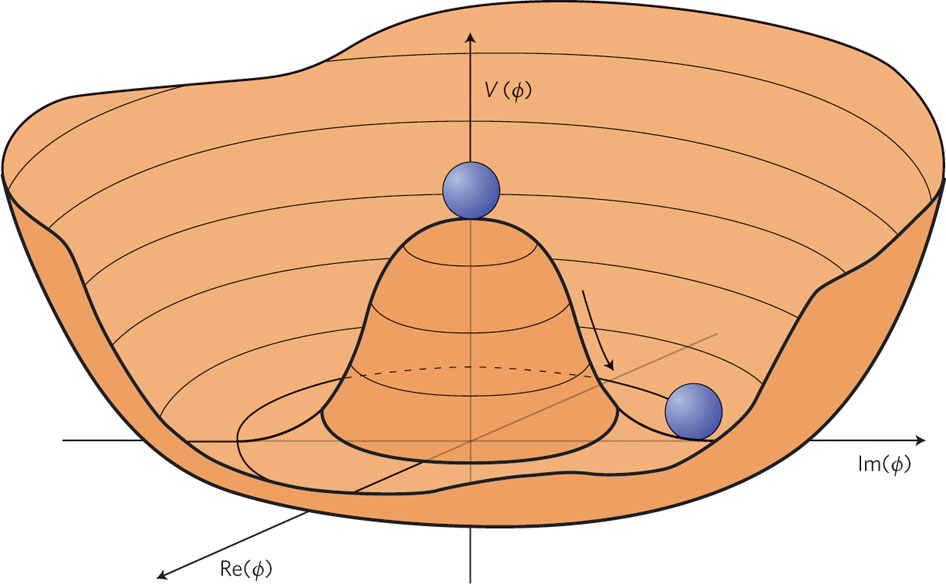
\includegraphics[width=0.9\textwidth]{StandardModel/higgs_potential.jpg}
\caption{\small An effective potential, V($\Phi$), that leads to spontaneous symmetry breaking.~\cite{Eyeonaprize2011} }
\label{fig:higgs_potential}
\end{figure}



\subsection{Higgs Boson Mass}

The Higgs boson mass is the only one of the 18 free parameters of the Standard Model~\cite{Englert1964} that was still undetermined at the start up of the LHC. While the mass of the Higgs boson is dependent on the parameters $\nu$ and $\lambda$, only $\nu$ can be estimated from another parameter.  Despite theoretically not being able to determine the Higgs boson mass, there are both theoretical and experimental constraints on the Higgs mass.  These come from both direct and indirect searches at various colliders.


\subsubsection{Theoretical Constraints}


The scalar potential needs to be bounded from below, even after including radiative corrections.  This gives a lower bound on $m_H$ as well.  If the quartic coupling $\lambda(\mu)$ stays positive then this requirement is fulfilled.  This is true at least until $\mu\sim\Lambda$ which is the maximum energy scale wherein the theory is still applicable~\cite{Ridolfi2001}. The relation $m_H^2\simeq 2\lambda(m_Z)v^2$ defines a $\Lambda$-dependent lower bound on $m_H$. This shows that for smaller values of $\lambda(m_Z)$ the $\Lambda$ scale also becomes smaller.  This leads to $\lambda$ becoming negative which means the scalar potential is no longer bounded.  The absolute minimum or vacuum stability is shown by the dashed line in figure~\ref{fig:bothbounds}. If the vacuum stability is only a local constraint we get a slightly looser lower bound as shown in the dot-dashed line in figure~\ref{fig:bothbounds}.


\begin{figure}[htb]
\centering
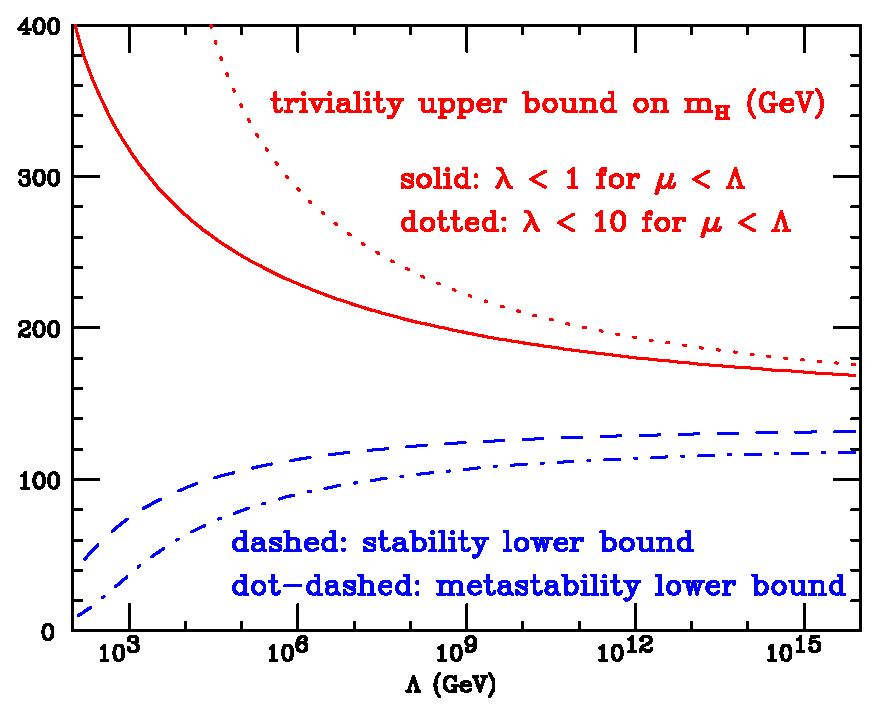
\includegraphics[width=0.9\textwidth]{StandardModel/bothbounds.eps}
\caption{Upper and lower bounds on the Higgs mass.~\cite{Ridolfi2001} }
\label{fig:bothbounds}
\end{figure}

% from the paper
%The smaller is $\lambda(m_Z)$, the smaller becomes the scale $\Lambda$ at which $\lambda$ becomes negative and the scalar potential unbounded. 
%Since $m_H^2\simeq 2\lambda(m_Z)v^2$, this implies a $\Lambda$-dependent lower bound on $m_H$.


The unitarity of the scattering matrix gives an upper bound on the Higgs mass.  This can be seen in the elastic scattering of $Z$ bosons, $Z Z \to Z Z$.  In the limit that $s\gg m_Z^2$ we have:
\begin{equation} {\cal M}=-\frac{m_H^2}{v^2}\left[\frac{s}{s-m_H^2}+\frac{t}{t-m_H^2}+\frac{u}{u-m_H^2}\right] \label{eq:unitarity1}\end{equation}

Now with $J=0$ then the amplitude of ${\cal M}$ gives us:
\begin{equation}|{\cal M}_0|^2\to\left[\frac{3}{16\pi}\frac{m_H^2}{v^2}\right]^2<\frac{s}{s-4m_Z^2}\label{eq:unitarity2}\end{equation}

Since we said that $s\gg m_Z^2$ we get that $m_H<\sqrt{\frac{16\pi}{3}}\,v\sim 1\;{\rm TeV}$. Similarly if we look at $Z W \to Z W$ then the limit is $\sim 800$~GeV. There is another more restrictive constraint that is called the triviality bound. This is found by requiring that $\lambda$ is finite all the way to the $\Lambda$ scale.  When these limits are taken to the grand unification scale or Plank scale ($\Lambda ~ 10^{19}$GeV) there is an extreme upper bound of 180 GeV~\cite{Ridolfi2001}.  Together with the extreme limits of the lower bound shows a Higgs mass should be in the range  of somewhere 130 GeV to 180 GeV as seen in Figure~\ref{fig:bothbounds}.  While this is a bit extreme, it does make sense for colliders to search up to a range of 1 TeV while focusing on the lower ranges.

\subsubsection{Experimental Constraints before the LHC}

In addition to the theoretical bounds, there were both direct and indirect measurements on the Higgs mass. Direct searches for the Higgs have mostly come from the Large Electron-Positron Collider (LEP) at CERN and the Tevatron at Fermilab~\cite{ALEPH:2010aa}. This search has been a driving force in high-energy experiments for the last several decades.  A brief overview of the constraints will be given below.
 Direct searches using data from LEP excluded the $m_H$ below 114.4 GeV at a 95\% C.L. ~\cite{Barate:2003sz}. LEP was an $e^+e^-$ accelerator that ran from 1989 to 2000. The main production mechanism at LEP was $e^+e^- \rightarrow Z^* \rightarrow ZH$ where a Higgs is radiated by a virtual Z boson.  This process is often referred to as ``Higgs-strahlung''.  The results can be seen in figure~\ref{fig:adlocls}.

\begin{figure}[htb]
\centering
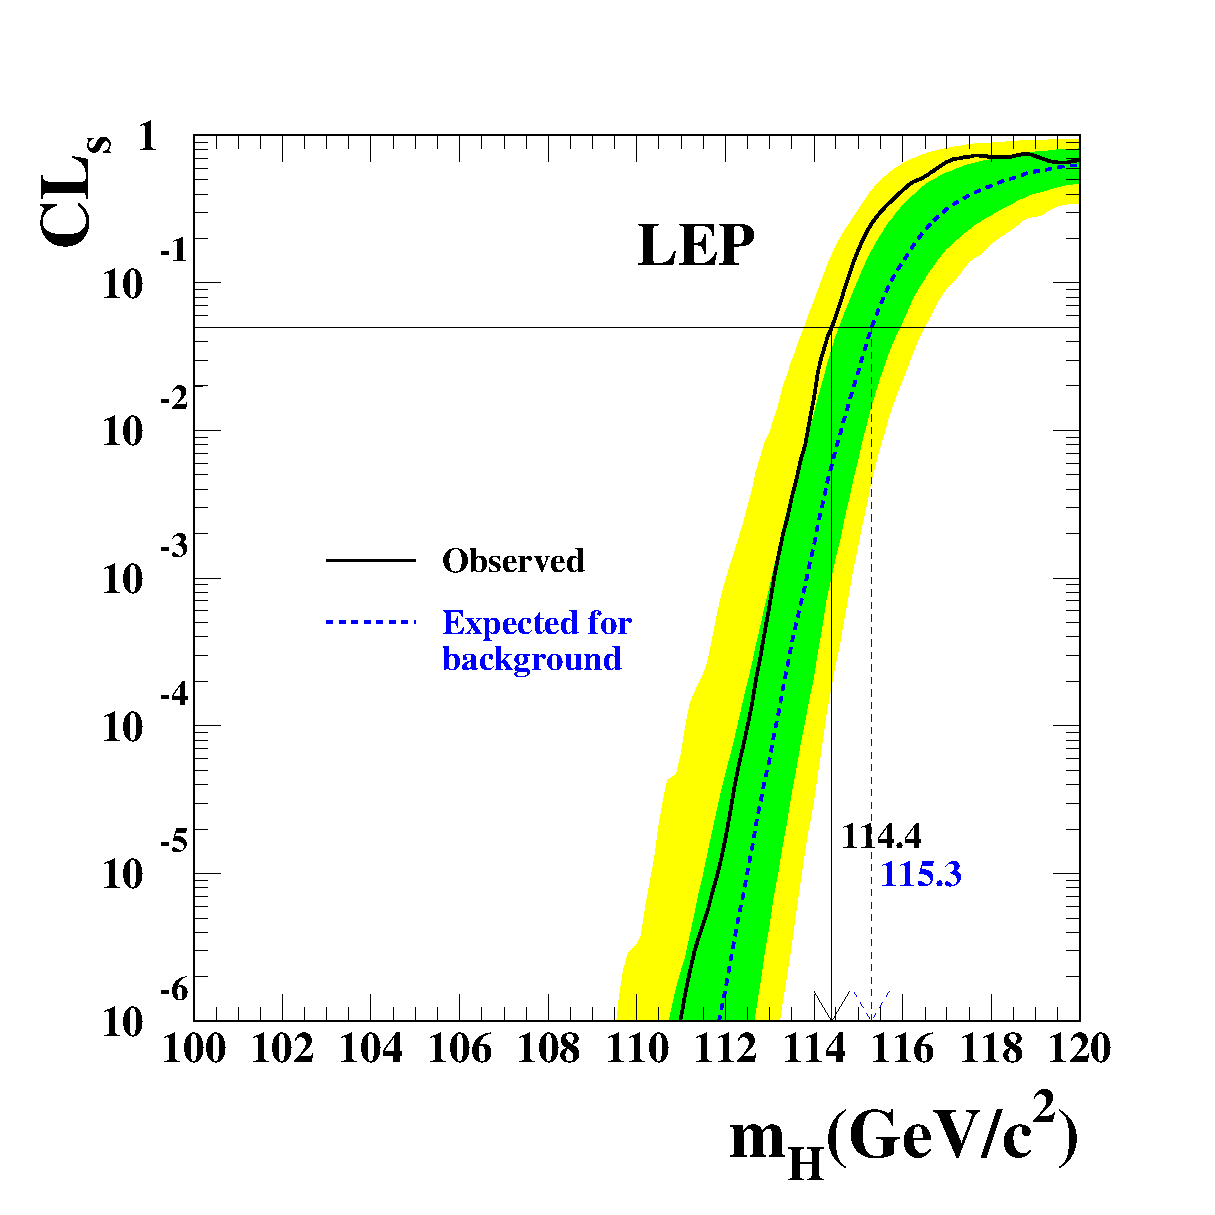
\includegraphics[width=0.7\textwidth]{StandardModel/fig9.eps}
\caption{\small The ratio $CL_S=CL_{(S+B)}/CL_B$
 for the signal plus background hypothesis. Solid line: observation; dashed line:
median background expectation. The dark and light shaded bands around the median
expected line correspond to the 68\% and 95\% probability bands. The intersection of the horizontal line 
for 
$CL_S = 0.05$
 with the observed curve is used to define the 95\%
confidence level
lower bound on the mass of the Standard Model Higgs boson.~\cite{Barate:2003sz} }
\label{fig:adlocls}
\end{figure}

The Tevatron, at Fermilab, was a proton-antiproton collider which took data up until 2011.  The center of mass energy of the Tevatron was 1.96 TeV.  The main mode of Higgs production studied at the Tevatron was $\Pp\Pap \rightarrow V\PH$ where $V$ is a vector boson $V\equiv \PWpm,\PZ$.  The decay products most studied is where the vector bosons decay into leptons.  The most promising Higgs decay was $\PH \rightarrow \PWp\PWm$ if the Higgs had a mass above 135 GeV.  The combination of the Tevatron results for the CDF and D$\emptyset$ experiments can be seen in Figure~\ref{fig:comboRatio}~\cite{CDFandD0:2011aa}. In addition to confirming part of the already excluded range from LEP, the range 149 to 182 GeV was excluded at the 95\% confidence level.

\begin{figure}[htb]
\centering
%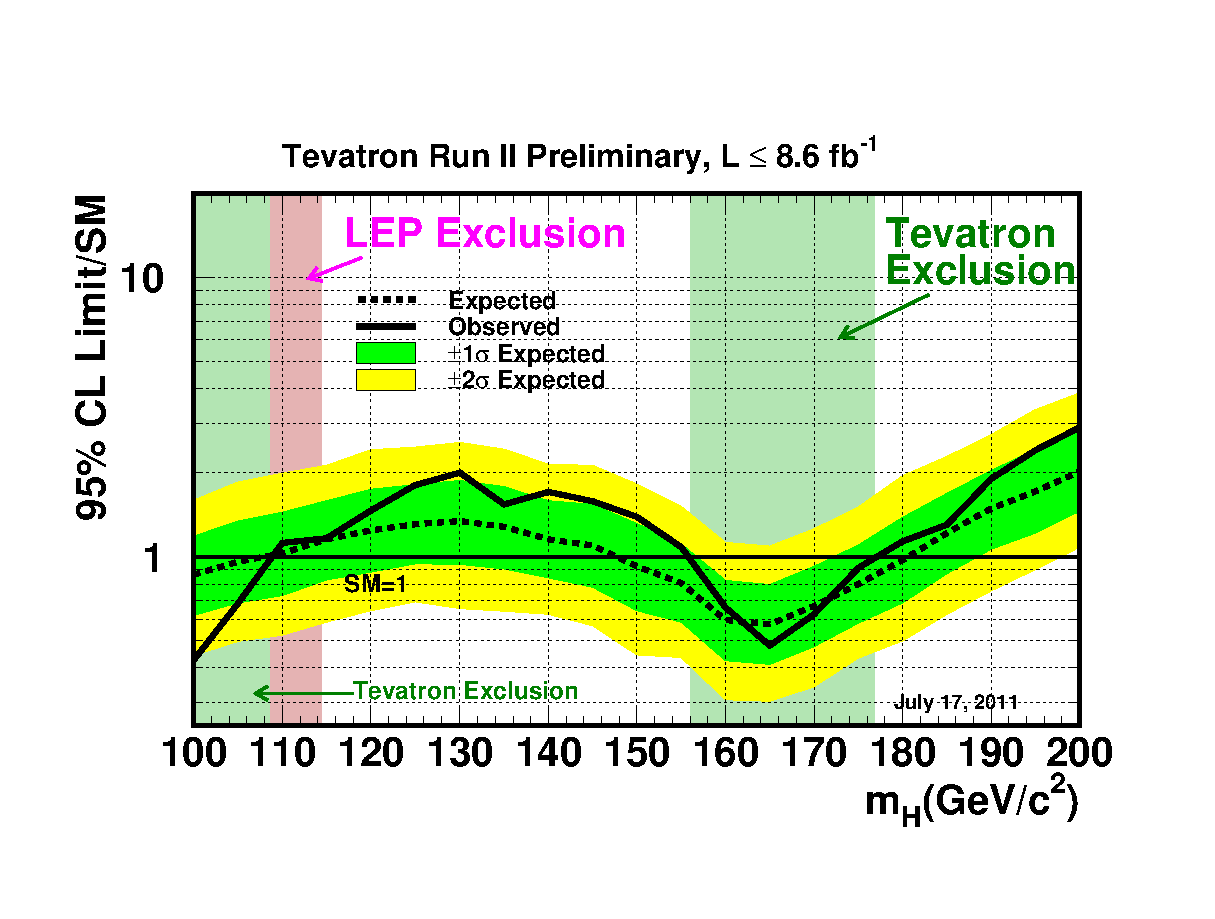
\includegraphics[width=0.8\textwidth]{StandardModel/tevbayeslimits17july2011.eps}
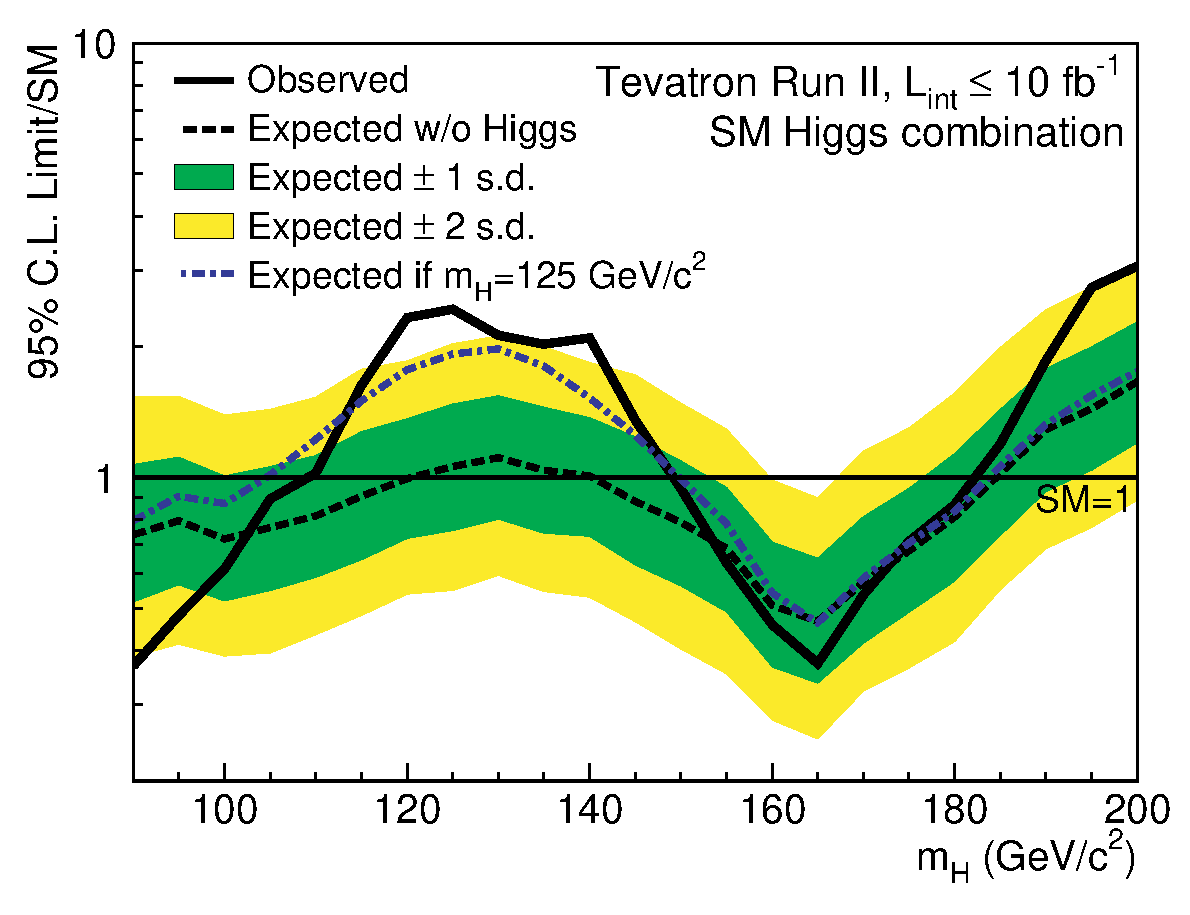
\includegraphics[width=0.8\textwidth]{StandardModel/tevsmlimits_feb2013.eps}
\caption{\small
Observed and median expected (for the background-only hypothesis) 95\% C.L. Bayesian upper production limits expressed as multiples of the SM cross section as a function of Higgs boson mass for the combined CDF and D0 searches in all decay modes. The dark and light shaded bands indicate, respectively, the 1 and 2 standard deviations probability regions in which the limits are expected to fluctuate in the absence of signal. The blue short dashed line shows median expected limits assuming the SM Higgs boson is present at m$_H$ = 125 GeV.~\cite{CDFandD0:2011aa}
%Also shown are the  expected upper limits obtained for
%all combined CDF channels, and for  all combined D0 channels.
}
\label{fig:comboRatio}
\end{figure}


Through fitting precision electroweak measurements, indirect measurements of the Higgs boson mass can be derived. Of particular usefulness is the changes in the vacuum polarization of the $\PZ$ and $\PWpm$ bosons through loop corrections. Figure~\ref{fig:indirect_greenband}~\cite{Flacher:2008zq} shows the $\Delta\chi^2$ variation of best fit to the combined data of LEP, Tevatron, and the Stanford Linear Accelerator (SLAC) accelerators, both with the pure indirect searches, and the combined direct and indirect searches.  While the lower Higgs masses are favored, even the high mass ranges were not completely ruled out.

\begin{figure}[htb]
\centering
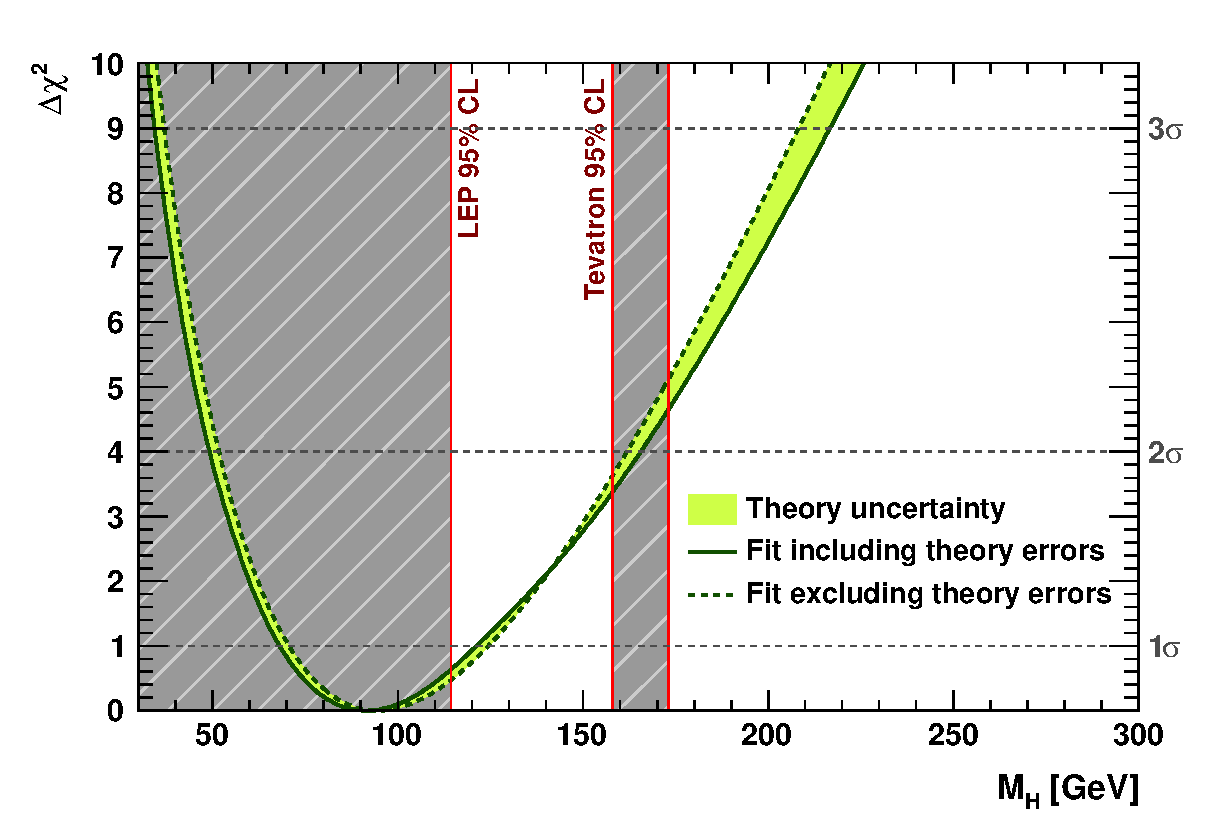
\includegraphics[width=0.7\textwidth]{StandardModel/HiggsScan.eps}
\includegraphics[width=0.7\textwidth]{StandardModel/HiggsScanDirectSearches.eps}
%   \centerline{\epsfig{file=Figures_Para/HiggsScanDirectSearches.eps, scale=\defaultFigureScale}}
%  \vspace{ 0.3cm}
\caption{\small Indirect determination of the Higgs boson mass: 
            $\Delta\chi^2$ as a function of $M_H$ for the standard fit (top) and the 
            complete fit (bottom). The solid (dashed) lines give the results when 
            including (ignoring) theoretical errors.~\cite{Flacher:2008zq}
         }
\label{fig:indirect_greenband}
\end{figure}






%\begin{fmffile}{simple}
%  \begin{fmfgraph}(40,25)
%    % Note that the size is given in normal parentheses
%    % instead of curly brackets.
%    % Define external vertices from bottom to top
%    \fmfleft{i1,i2}
%    \fmfright{o1,o2}
%    \fmf{fermion}{i1,v1,o1}
%    \fmf{fermion}{i2,v2,o2}
%    \fmf{photon}{v1,v2}
%  \end{fmfgraph}
%\end{fmffile}
%
%	    \begin{fmffile}{gluon}
%	        \begin{fmfgraph}(40,25)
%	            \fmfleft{in}
%	            \fmfright{out}
%	            \fmf{curly}{in,out}
%	        \end{fmfgraph}
%	    \end{fmffile}



%Within the framework of relativistic quantum field theory the Standard Model is a description of the microscopic world in terms of interaction particles and fields.\cite{Ryder1996} It can be divided into two parts: quantum chromodynamics (QCD) and quantum electrodynamics (QED). This allows us to write the Lagrangian as the summation of two separate parts:
%\begin{equation}
%\mathcal{L}_{SM} = \mathcal{L}_{QED} + \mathcal{L}_{QCD}
%\label{eq:sum_lagrandian}
%\end{equation}
%In QED the unphysical infinite contributions can always be eliminated.  This means that the theory is renormalizable. The Standard Model is renormalizable and also is compatible with special relativity. In 1960 Sheldon Glashow combined electromagnetism and weak interactions together to form the basis of the electroweak theory of interactions.\cite{Glashow1961} 



%\section{The Higgs Mechanism}

%If a doublet of scalar fields is introduced then its self-interactions provide spontaneous symmetry breaking and give masses to the gauge and fermion fields. This addition to the Lagrangian is $\mathcal{L}_{\Phi}$ and $\mathcal{L}_{\Phi}^F$ which are described in Equation ~\ref{eq:lagrangian_scalar}. It also introduces the Higgs boson, a new neutral scalar particle. 
%\begin{equation} \mathcal{L}_{\Phi} = |D_{\mu}\Phi|^2 - V(|\Phi|^2) \label{eq:lagrangian_scalar}\end{equation}
%For the scalar potential V the most general form that is renormalizable is Equation ~\ref{eq:potential_V}.
%\begin{equation} V = \mu^2|\Phi|^2 + \lambda|\Phi|^4 \label{eq:potential_V}\end{equation}

%From this the Higgs mechanism allows the vacuum to emit or absorb a Higgs boson. The coupling of the W and Z bosons to the Higgs field effectively gives them mass, while because the photon and gluon cannot couple to it they remain mass-less.

\section{The LHC Higgs Boson Search}

\subsection{LHC Higgs Production}

The Large Hadron Collider (LHC) at CERN is a proton-proton (pp) collider.  It had a center of mass energy of 7 TeV in 2010-2011 which increased to 8 TeV in 2012.  It reached an instantaneous luminosity of approximately $5 \times 10^{33} cm^{-2}s^{-1}$ ~\cite{1748-0221-3-08-S08001} in 2012.  There are four Higgs production processes at the LHC which are listed in Table~\ref{tab:lhc_higgs_production} in order of decreasing cross section.  The corresponding Feynman diagrams are in Figure~\ref{fig:Higgs_Feynman_diag} ~\cite{Egede_Feynman_Higgs}.  The cross sections for each of these processes at both $\sqrt{s}$ = 7 TeV and $\sqrt{s} =$ 8 TeV can be seen in Figure~\ref{fig:LHC_higgs_production} ~\cite{LHC_Higgs_Gallery}. It is important to note that changing from 7 TeV to 8 TeV increased the inclusive Higgs boson production cross-section at $m_H$ = 125 GeV by about 25\%. 

Gluon-gluon fusion is the dominant Higgs production process at the LHC center of mass energies. Vector boson fusion (VBF) is the second largest production cross section and is about one order of magnitude less than gluon gluon fusion.  In the very high mass region the processes become more comparable.  Despite this lower cross section, VBF is extremely powerful because of the two spectator jets that have a large invariant mass.  This signature allows good background discrimination. The following analysis mainly deals with these two processes. 



\begin{table}[htb]
\caption{%
  \small Higgs production processes at the LHC. %
}
\begin{center}
\begin{tabular}{ | c | c | }
\hline
gluon gluon fusion & $\Pg\Pg \rightarrow \PH$ \\ \hline
vector boson fusion & $\Pq\Pq \rightarrow \PH\Pq\Pq$ \\ \hline
associated production & $\Pq\Paq \rightarrow \PW\PH,\PZ\PH$ \\ \hline
associated production with top quarks & $gg,\Pq\Paq \rightarrow \Pqt\Paqt\PH$ \\ \hline
\end{tabular}
\end{center}
\label{tab:lhc_higgs_production}
\end{table}

\begin{figure}[htb]
\centering
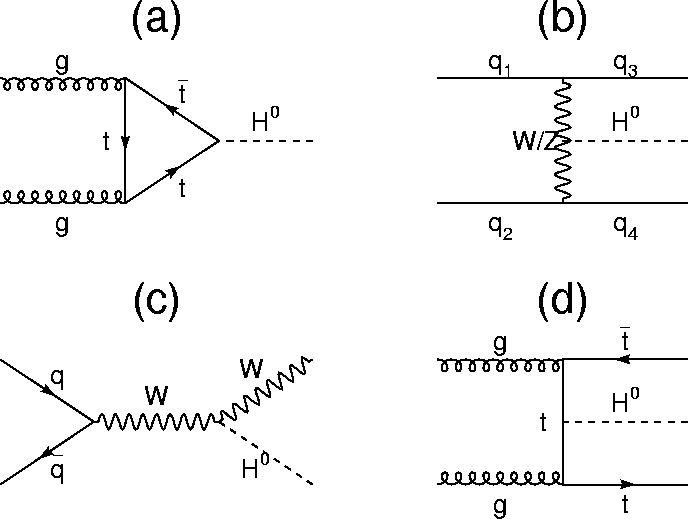
\includegraphics[width=0.7\textwidth]{StandardModel/feynman_higgs_production.jpg}
%   \centerline{\epsfig{file=Figures_Para/HiggsScanDirectSearches.eps, scale=\defaultFigureScale}}
%  \vspace{ 0.3cm}
\caption{\small The most important processes for Higgs production at hadron colliders. Gluon fusion (a), vector boson fusion (b), Associative production with W (c) and an example of the diagrams having associative production with a top pair (d). ~\cite{Egede_Feynman_Higgs}
         }
\label{fig:Higgs_Feynman_diag}
\end{figure}


\begin{figure}[htb]
\centering
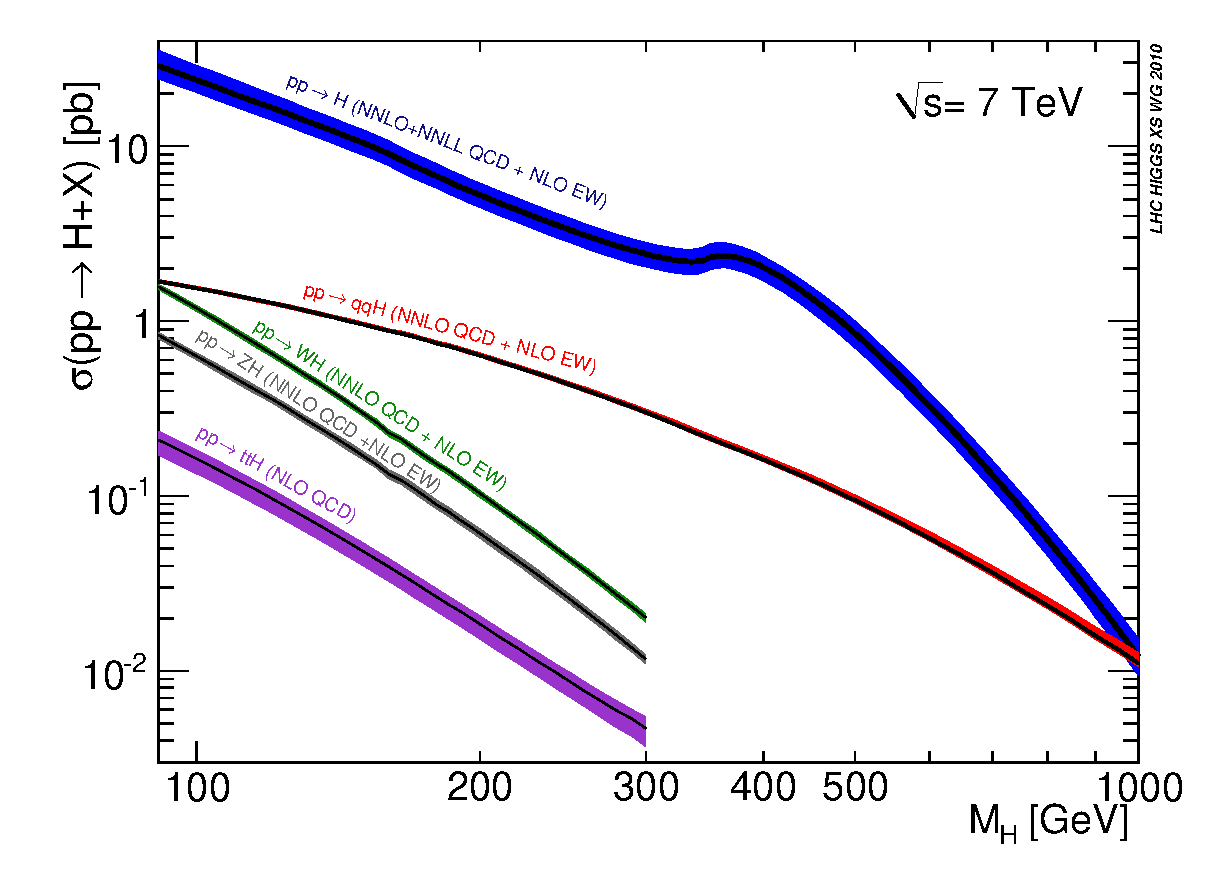
\includegraphics[width=0.7\textwidth]{StandardModel/Higgs_XS_7TeV.eps}
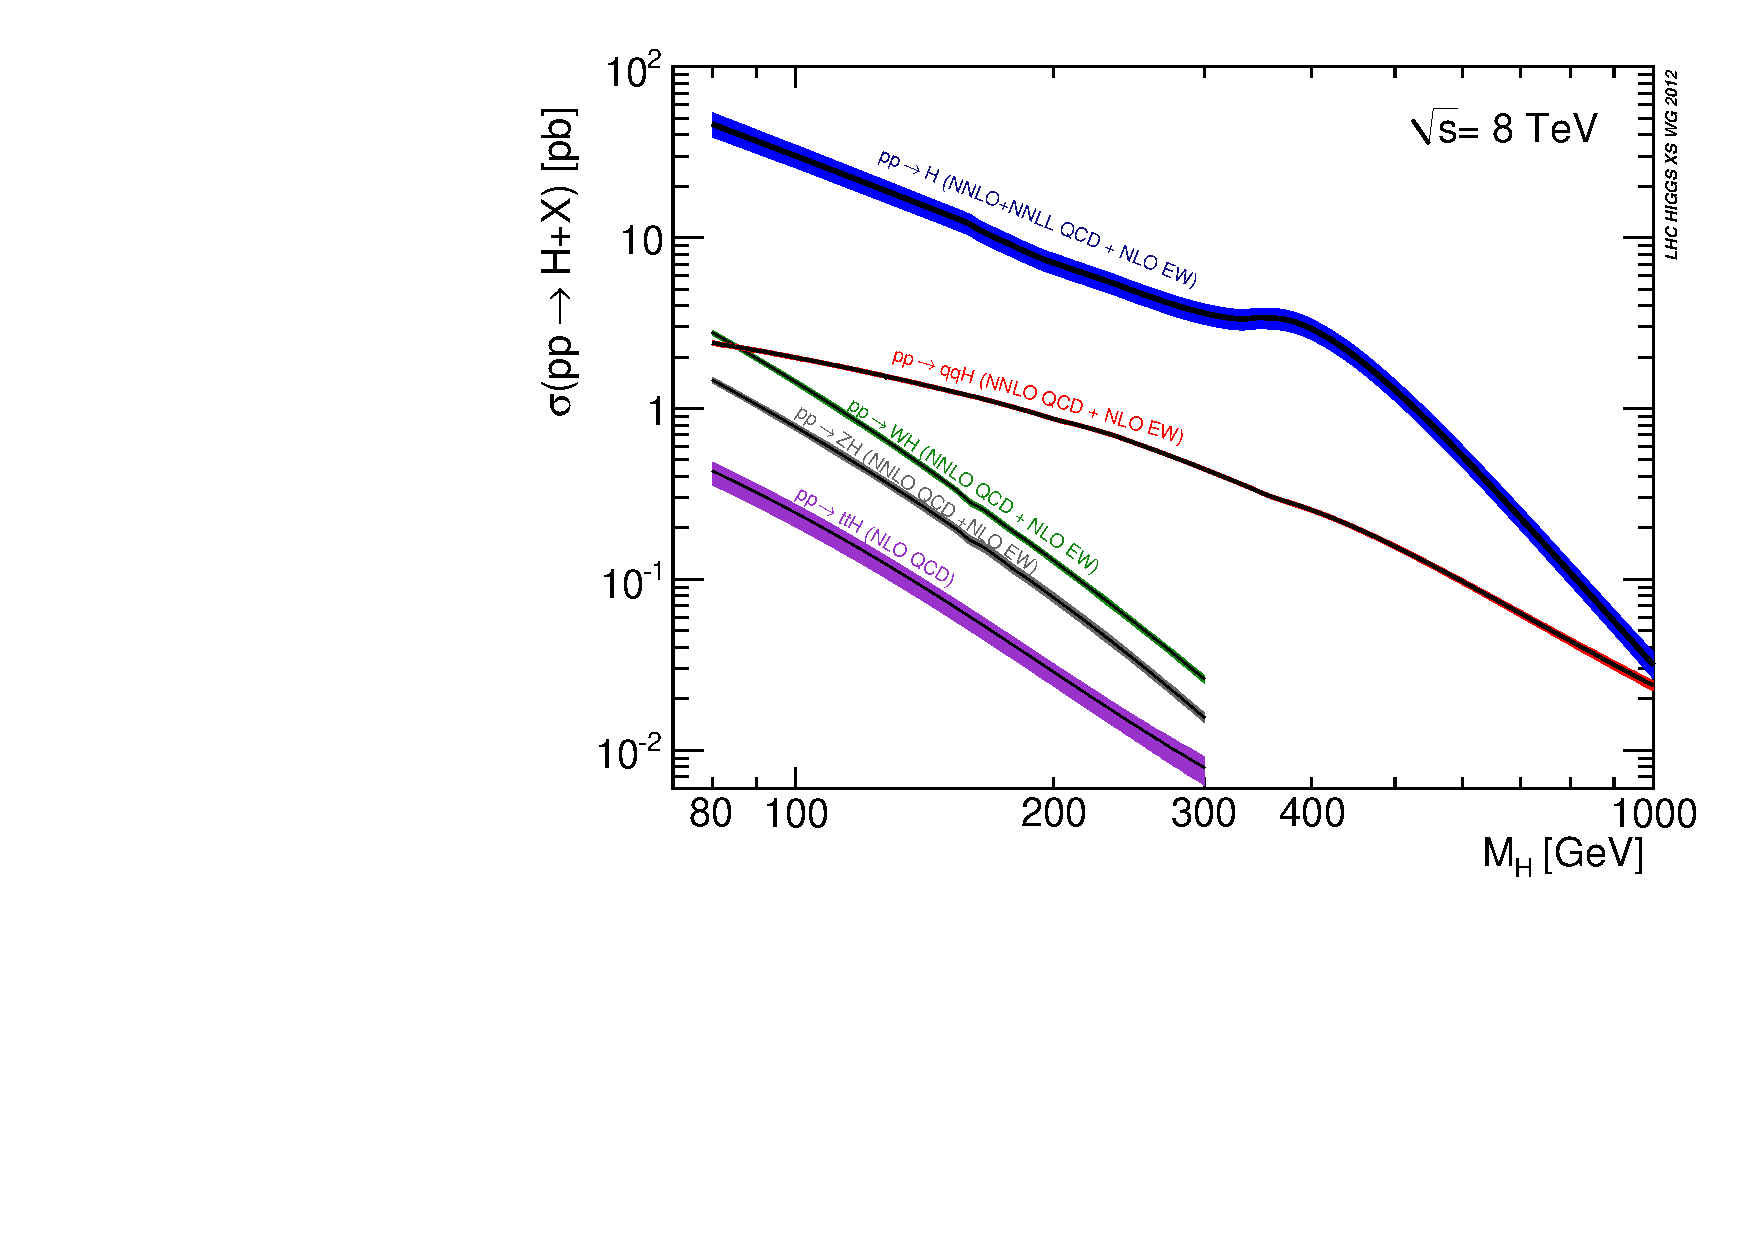
\includegraphics[width=0.7\textwidth]{StandardModel/Higgs_XS_8TeV_lx.pdf}
\caption{\small Standard Model Higgs boson production cross sections at $\sqrt{s}$ = 7, 8 TeV. Transition for VBF at MH=300 GeV at 8 TeV is due to change from ZWA to complex-pole-scheme.~\cite{LHC_Higgs_Gallery}
         }
\label{fig:LHC_higgs_production}
\end{figure}

\subsection{Higgs Decay}

The Higgs boson can decay into a variety of other particles.  The branching ratios of this decay are shown in Figure~\ref{fig:Higgs_decay}~\cite{LHC_Higgs_Gallery}.  From these images we can see that in the low mass region the most important decays are the fermions with $\PH \rightarrow \Pqb\Paqb$.  This is most important because the b quark is the heaviest fermion into which the decay is kinematically allowed. As soon as it is possible to create vector boson pairs they begin to dominate the branching fraction.  Also in the high mass region (above 350 GeV) $\Pqt\Paqt$ pairs are created.  An important thing to note is that the best Higgs decay channels are not only those with large branching ratios, but also those in which a good signal to background ratio can be achieved. There are three Higgs mass regions that have different properties in this respect.


\begin{figure}[htb]
\centering
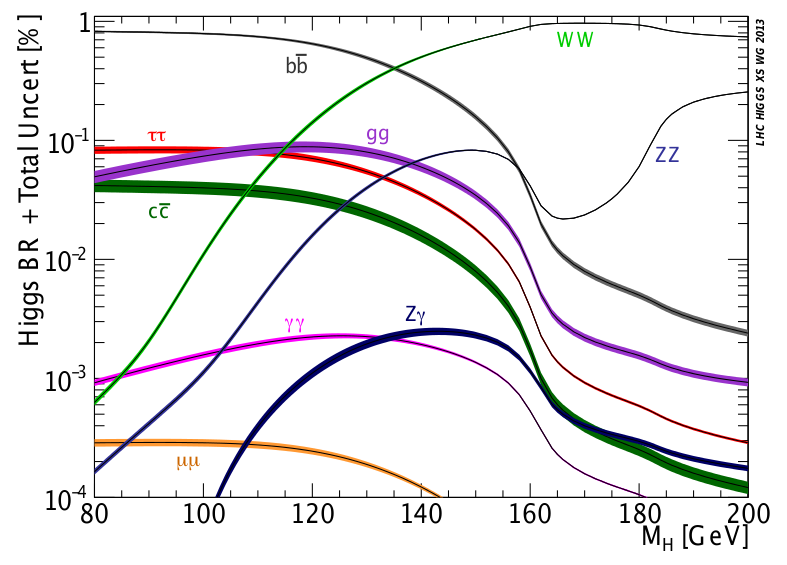
\includegraphics[width=0.8\textwidth]{StandardModel/Higgs_BR_LM_RECT.png} 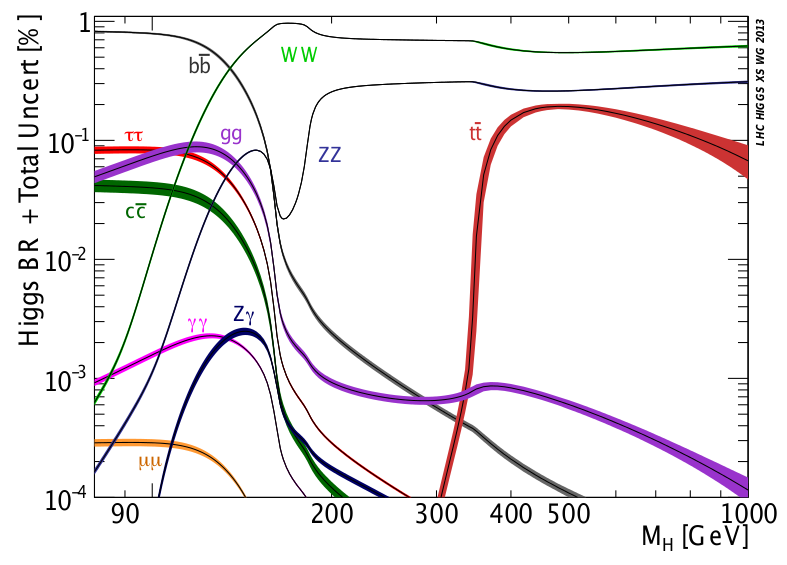
\includegraphics[width=0.8\textwidth]{StandardModel/Higgs_BR_RECT.png}
\caption{\small Standard Model Higgs boson decay branching ratios for two different $m_H$ ranges. ~\cite{LHC_Higgs_Gallery}
         }
\label{fig:Higgs_decay}
\end{figure}


In the low mass region ($m_H < 120$ GeV), even though the dominant decay is $\PH \rightarrow \Pqb\Paqb$, the bb di-jet backgrounds make this channel extremely difficult to use.  The most promising channel is the $\PH \rightarrow \Pgg\Pgg$.  The reason this channel works well is because the signature is so clear and there are only the $\Pq\Paq \rightarrow \Pgg\Pgg$ and the $\PZ \rightarrow \Pep\Pem$ backgrounds.  In the mid mass region (120 GeV $< m_H <$ 135 GeV) $\PH \rightarrow \Pgg\Pgg$ is still available but also $\PH \rightarrow \PW\PW^*, \PZ\PZ^*, \PZ\Pgg$. The real winner of these is the $\PH \rightarrow \PZ\PZ^* \rightarrow 4\Pl$ because even though it has a lower branching ratio than $\PW\PW^*$, it has a very clear decay signature and is able to fully reconstruct the Higgs mass.  In the high mass region ($m_H >$ 135 GeV) both the $\PW\PW$ and $\PZ\PZ$ channels begin to dominate.  Despite the lower branching ratio of the  $H \rightarrow \PZ\PZ$ decay, the clean signature allows good background rejection.


\subsection{H $\rightarrow$ ZZ $\rightarrow l^{+}l^{-} \Pq \Paq$ Channel}
In the high mass region for a Higgs boson discovery the predominant Higgs decay is to vector boson pairs, H $\rightarrow$ WW and H $\rightarrow$ ZZ.  The signatures from the fully leptonic decay modes for these two processes are easily reconstructible and can be distinguished from the background processes.  The fully leptonic decay modes are H $\rightarrow$ WW $\rightarrow$ $l^{+} \Pgn l^{-} \Pagn$ and H $\rightarrow$ ZZ $\rightarrow$ $l^{+}l^{-}l^{+}l^{-}$. The H $\rightarrow$ ZZ $\rightarrow$ $l^{+}l^{-}l^{+}l^{-}$ channel is particularly interesting because the decay chain can be fully reconstructed with a narrow invariant mass peak and almost no Standard Model background. The rate of decay of Z $\rightarrow$ $l^{+}l^{-}$ is only 3.37\% \cite{PDG2012} so for $ l = e,\Pgm$ there is only a 0.45\% chance of ZZ $\rightarrow$ $l^{+}l^{-}l^{+}l^{-}$.

The largest Z branching ratio is 69.9\% for Z $\rightarrow \Pq \Paq$ \cite{PDG2012}. Furthermore, ZZ $\rightarrow \Pq \Paq \Pq \Paq$ has a decay probability of just under 50\%. The problem is that while this maximizes the branching ratio, this final state is indistinguishable from Standard Model background processes, like QCD.

The semi-leptonic final state in H $\rightarrow$ ZZ $\rightarrow l^{+}l^{-} \Pq \Paq$ produces a number of benefits over the previous two decay channels.  The branching ratio of ZZ $\rightarrow l^{+}l^{-} \Pq \Paq$ is 9.4\%, or more than 20 times as large as ZZ $\rightarrow$ $l^{+}l^{-}l^{+}l^{-}$. This can be seen in the plots of Higgs decay cross section multiplied by the final state branching ratio for both 7 TeV and 8 TeV in Figure~\ref{fig:XSBR}~\cite{LHC_Higgs_Gallery}. In comparison to ZZ $\rightarrow \Pq \Paq \Pq \Paq$ the leptonic decay of one of the Z bosons significantly reduces the Standard Model background in the final state.

\begin{figure}[htb]
\centering
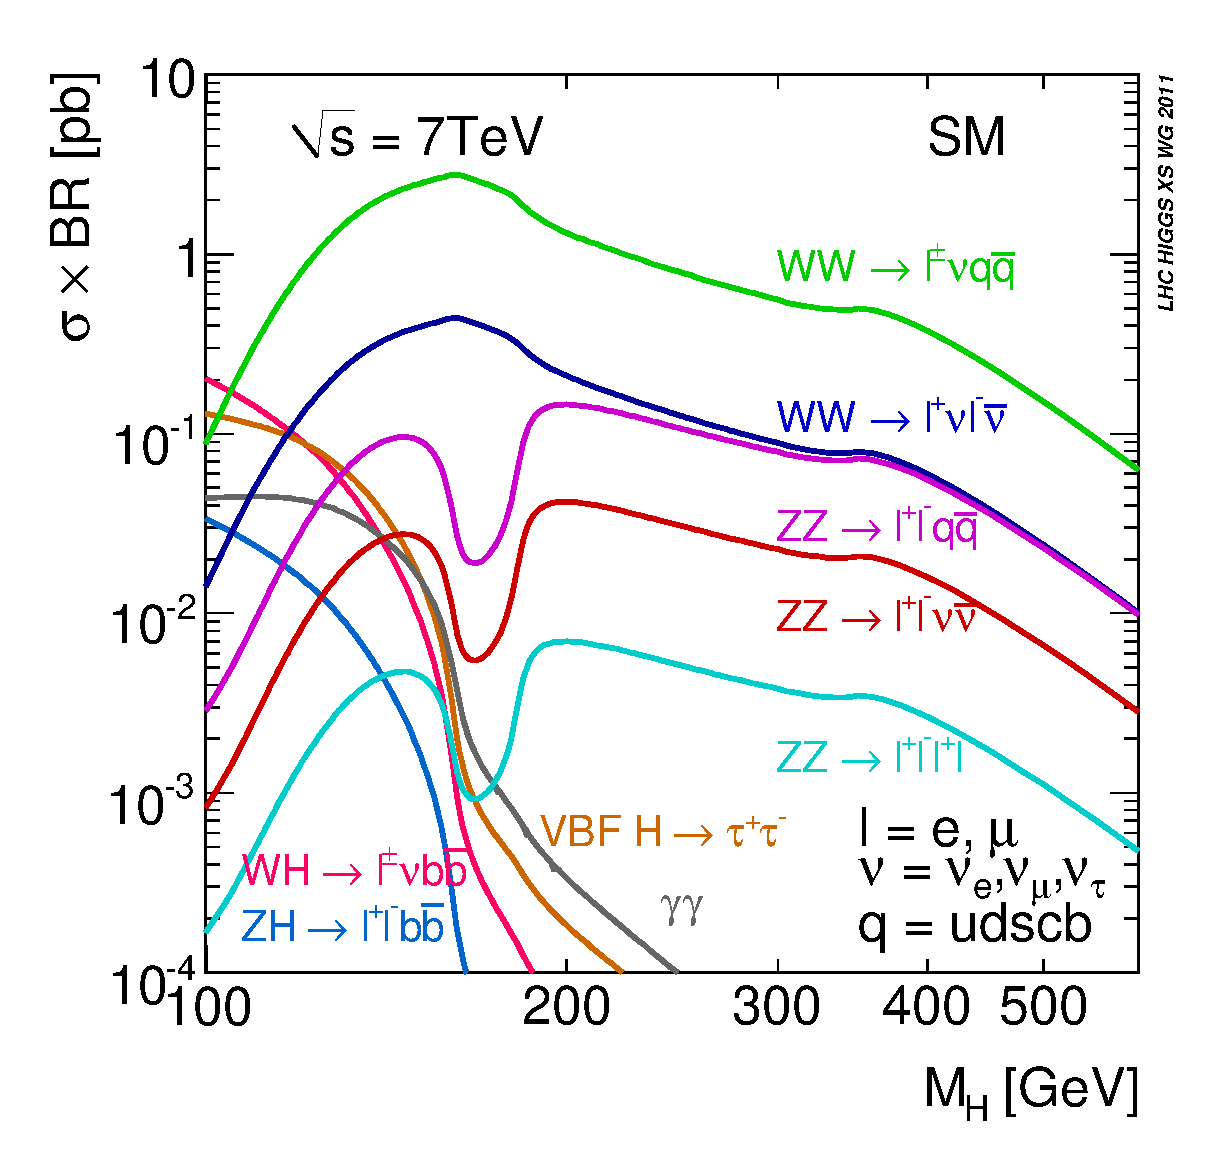
\includegraphics[width=0.7\textwidth]{StandardModel/XSBR_7TeV_SM.eps} 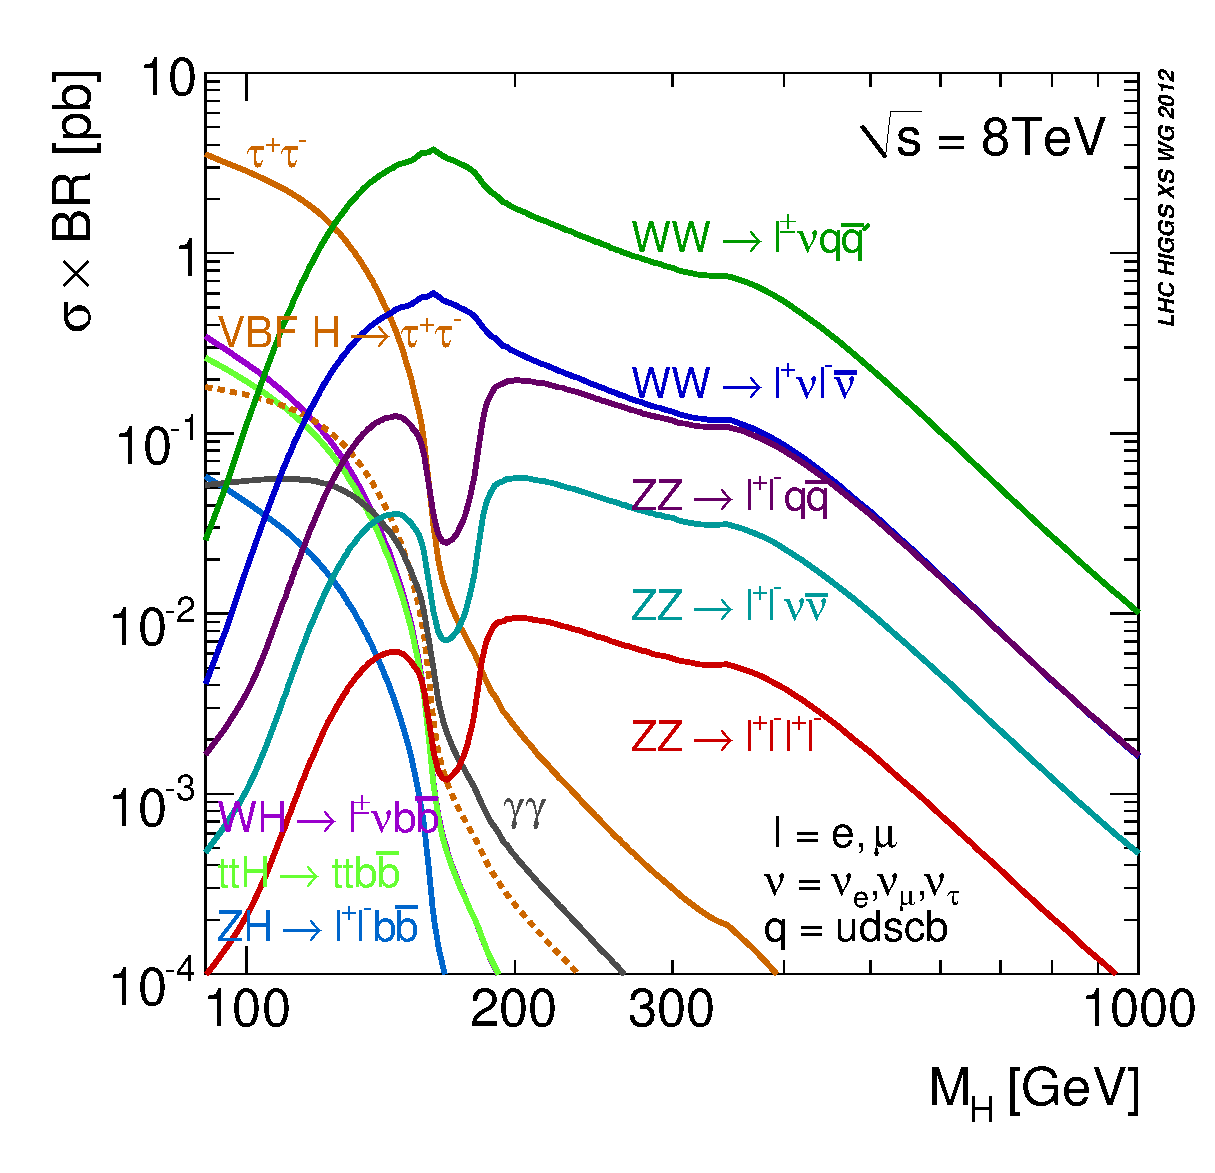
\includegraphics[width=0.7\textwidth]{StandardModel/XSBR_8TeV_SM_HM.eps}
\caption{\small Standard Model Higgs boson production cross section times branching ratio at $\sqrt{s}$ = 7 TeV and 8 TeV. ~\cite{LHC_Higgs_Gallery}
         }
\label{fig:XSBR}
\end{figure}



Some of the difficulties in this channel compared to the fully leptonic decay are increased difficulty in event selection, the final reconstruction efficiency is approximately half of the fully leptonic final state, the backgrounds are significantly higher and dominated by Z+jets final states, and the resolution is worse.  Despite these difficulties, this channel has improved sensitivity over the fully leptonic final state at high masses because of the higher branching ratio that the semi-leptonic final state enjoys, and at high masses the Z+jets background is not as significant.



\subsubsection{$l^{+}l^{-} \Pq \Paq$ Background Contamination}

The background processes for this channel are processes which have a pair of oppositely charged leptons with large transverse momentum that are associated with two jets.  The main backgrounds are listed in Table~\ref{tab:background_2l2q}.

\begin{table}[htb]
\caption{%
  The main Standard Model background processes for the H $\rightarrow$ ZZ $\rightarrow l^{+}l^{-} \Pq \Paq$ channel and their cross sections at 8 TeV.
}
\begin{center}
  \begin{tabular}{ | c | c |} \hline
    Background Process & Cross Section [pb] at 8 TeV\\ \hline \hline
    $\PZ + jets$ & 3503.71 \\ \hline
    $\Pqt \Paqt$ & 225.197\\ \hline
  %  $\Pqt \PWm$  & \\ \hline
  %  $\Paqt \PWp$ & \\ \hline
    $\PZ \PZ$    & 17.654 \\ \hline
    $\PW \PZ$    & 22.88 \\ \hline
    $\PW \PW$    & 57.1097\\ \hline
  \end{tabular}
\end{center}
\label{tab:background_2l2q}
\end{table}

The dominant background in the  $\PH \rightarrow \PZ\PZ \rightarrow l^{+}l^{-} \Pq \Paq$ analysis is the Z+jets background, or more specifically, the inclusive $\PZ$ production with QCD jets.  The cross section of Z production at the LHC is more than 10$^{4}$ larger than the Higgs signal.

Events containing top quarks are another significant source of background.  There are two top processes that result in the same final state as the signal we are studying.  They include $\Pqt \Paqt$ pair production and top quark associated production with a $\PW$ boson.
\begin{center}
  \begin{tabular}{ c }
    $\Pqt \Paqt  \rightarrow (\PWp \rightarrow \Plp\Pgn)\Pqb (\PWm \rightarrow \Plm\Pagn)\Paqb           $
  \end{tabular}
\end{center}



\chapter{Experimental Apparatus}

This chapter describes the Large Hadron Collider (LHC) and the Compact Muon Solenoid (CMS) detector.


\section{The Large Hadron Collider}

The parts of the Standard Model that we least understand are the electroweak spontaneous symmetry breaking and the Higgs field.  As referred to in the previous sections, direct searches for the Higgs boson in the past have failed. The verification of the full Standard Model, including the discovery of the Higgs boson, is one of the main goals of physics, as well as the LHC.  Despite this being an important goal, the LHC has many other processes that it is sensitive to, including new physics. Figure~\ref{fig:lhcall} shows the predictions for some important Standard Model cross sections at  $p \bar p$ and  $pp$  colliders~\cite{Campbell:2006wx}. 

\begin{figure}[htb]                                                               
\begin{center}
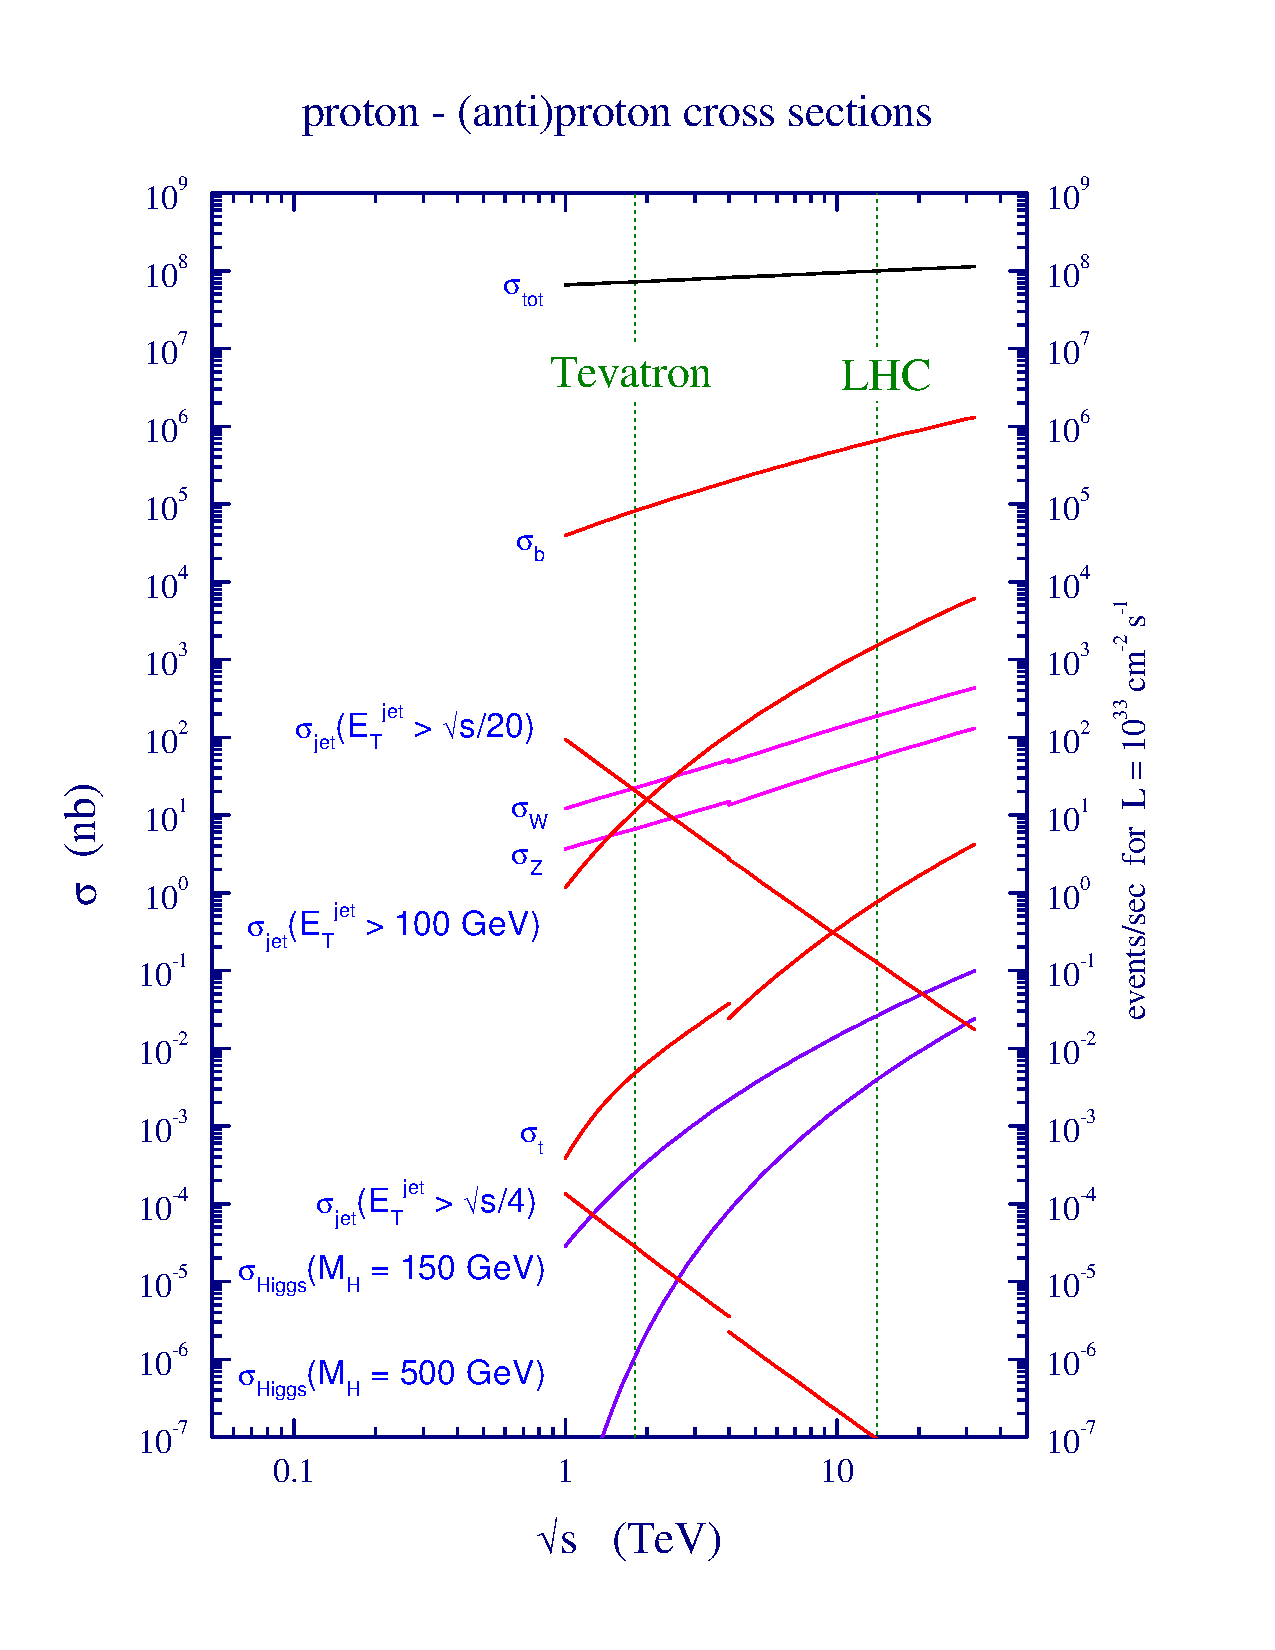
\includegraphics[width=0.99\textwidth]{Experiment/lhcolor.pdf}
\end{center}
\vspace*{-1cm}
\caption{Standard Model cross sections at the Tevatron
and LHC colliders.~\cite{Campbell:2006wx}}
\label{fig:lhcall}                    
\end{figure} 



The LHC accelerator is 26.7 km long and occupies the tunnel where the LEP collider was originally built.  This tunnel is located approximately 100 meters underground and spans the French and Swiss boarders near Geneva, Switzerland.  It is a proton-proton collider. The LHC is the world's largest and most powerful particle accelerator~\cite{LHCDesignReport}.

The LHC injection starts with the Linac2 to bring protons to 50 MeV.  After the Proton Synchrotron (PS) accelerates them to 1.4 GeV, the Super Proton Synchrotron (SPS) then injects the protons into the LHC at an energy of 450 GeV.  To finish, the LHC increases the energy 0.5 MeV per cycle until they are at 4.0 TeV.  This can be seen schematically in Figure~\ref{fig:lhc_schematic}~\cite{CERN_complex}. The LHC can also accelerate lead ions.

\begin{figure}[htb]
\centering
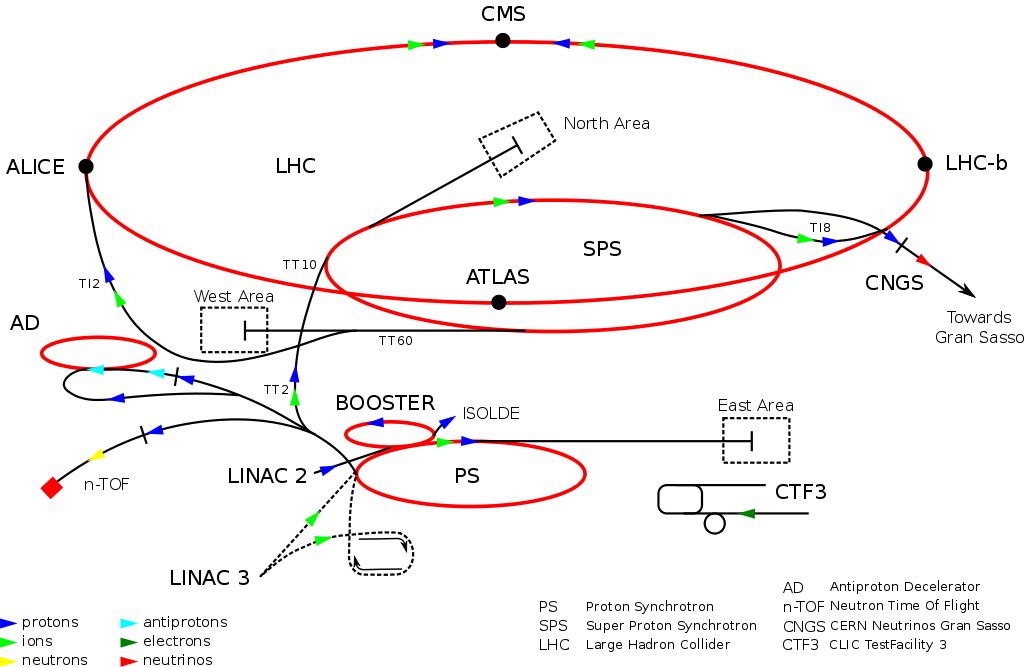
\includegraphics[width=0.99\textwidth]{Experiment/1024px-Cern-accelerator-complex.png}
\caption{Map of the CERN accelerator complex.\cite{CERN_complex}}
\label{fig:lhc_schematic}
\end{figure}

Because the protons being collided have the same electric charge, there are two vacuum chambers for acceleration with two different magnetic fields. There are 1,232 superconducting Niobium-Titanium magnets. Each one is 14.2 meters long and is cooled to 1.9 K with liquid Helium. The magnetic field produced is approximately 8.3 Tesla. These magnets are placed in 8 separate curved sections.

There are 4 interaction points in the LHC.  Two are high luminosity points at the general purpose experiments of A Toroidal LHC Apparatus (ATLAS) \cite{ATLASExperiment} and CMS. The other two are for the A Large Ion Collider Experiment (ALICE) \cite{ALICEExperiment}  and LHCb \cite{LHCbExperiment} experiments. These experiments can be seen in Figure~\ref{fig:lhc_experiments}.








\begin{figure}[htb]
\centering
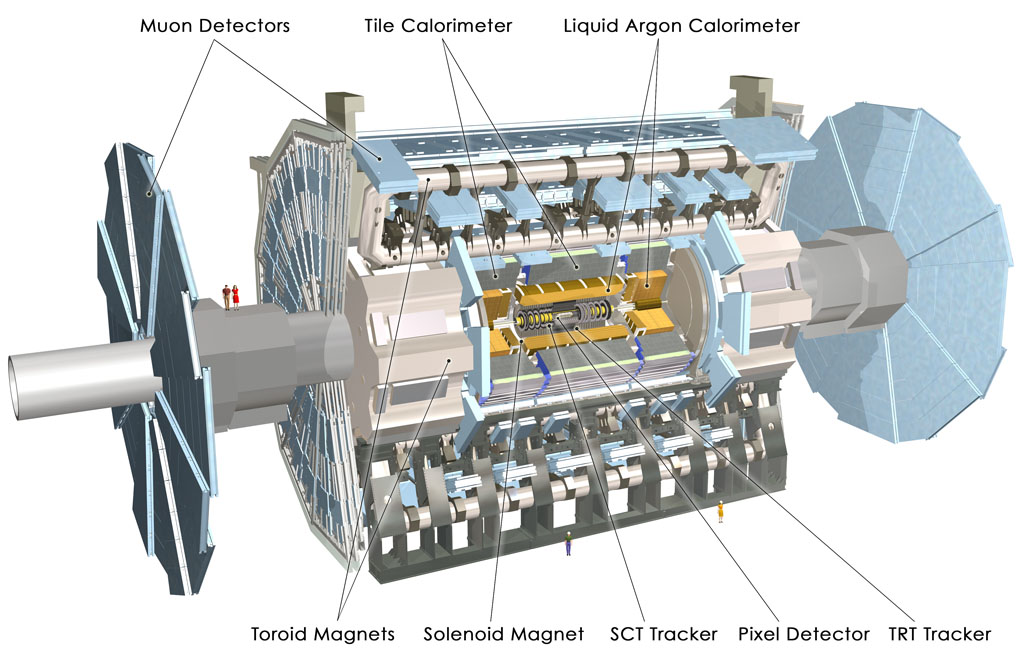
\includegraphics[width=0.49\textwidth]{Experiment/atlas.jpg}
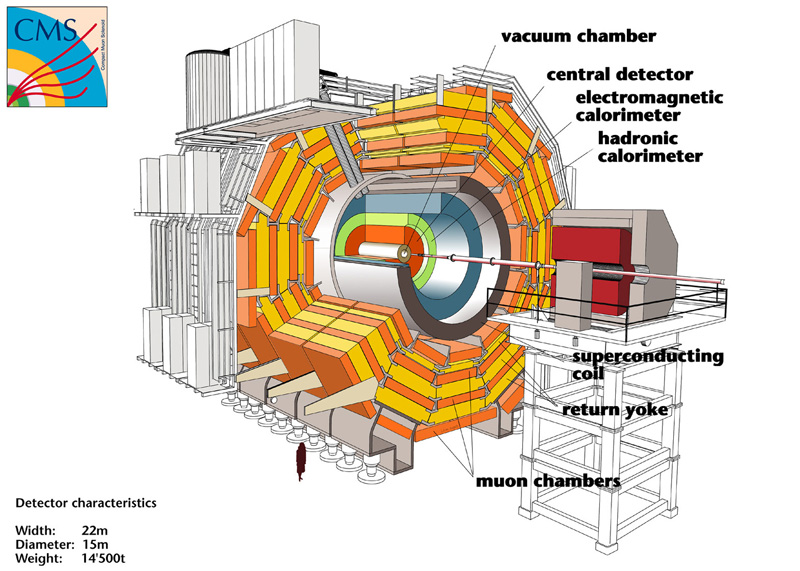
\includegraphics[width=0.49\textwidth]{Experiment/cms.jpg}
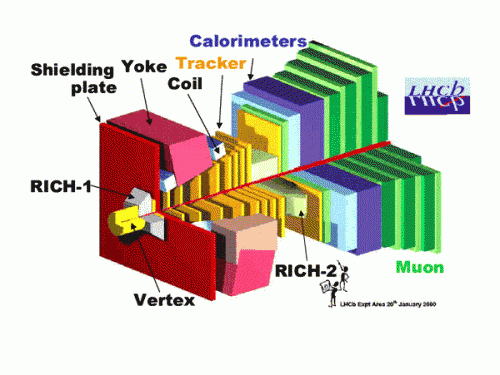
\includegraphics[width=0.49\textwidth]{Experiment/LHCb.png}
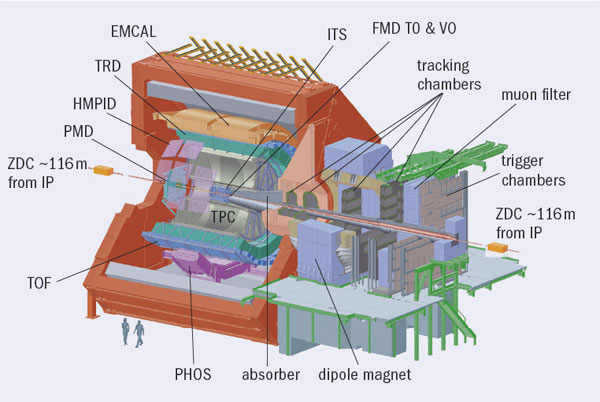
\includegraphics[width=0.49\textwidth]{Experiment/alice.jpg}
\caption{Top left: ATLAS experiment~\cite{ATLAS_image}. Top right:CMS experiments~\cite{CMS_image}. Bottom left: LHCb experiment~\cite{lhcb_image}. Bottom right: ALICE experiment~\cite{ALICE_image}.}
\label{fig:lhc_experiments}
\end{figure}




On November 23, 2009, the first proton-proton collisions were generated.  After a few runs at 450 GeV and 1.18 TeV beam energies, the first 7 TeV center-of-mass energies were achieved on March 30, 2010. This was the highest ever reached at a man made particle collider.  At 7 TeV approximately 47 $pb^{-1}$ of integrated luminosity were delivered in 2010 (see Figure~\ref{fig:lhc_luminocity}). The maximum instantaneous luminosity was $2 \times 10^{32} cm^{-2}s^{-1}$.

During 2011 the machine was only offline for short amounts of time.  On October 26, 2011 the highest ever instantaneous luminosity was reached with a peak value of $3.5 \times 10^{33} cm^{-2} s^{-1}$.  This was 1,331 bunches per beam with collisions every 50 ns. The total integrated luminosity delivered was 5.73 $fb^{-1}$ (see Figure ~\ref{fig:lhc_luminocity}). In 2012 the beam energy was increased to 4 TeV and the LHC continued to perform amazingly, ultimately delivering over 23 $fb^{-1}$ (see Figure~\ref{fig:lhc_luminocity}).

In the coming years the LHC will continue to increase it's energy and instantaneous luminosity.  Eventually it will reach the designed energy of 14 TeV collisions and an instantaneous luminosity of $10^{34} cm^{-2}s^{-1}$.  This is seven times the energy of the highest Tevatron energy and two orders of magnitude more luminosity of any previous experiment.



\begin{figure}[htb]
\centering
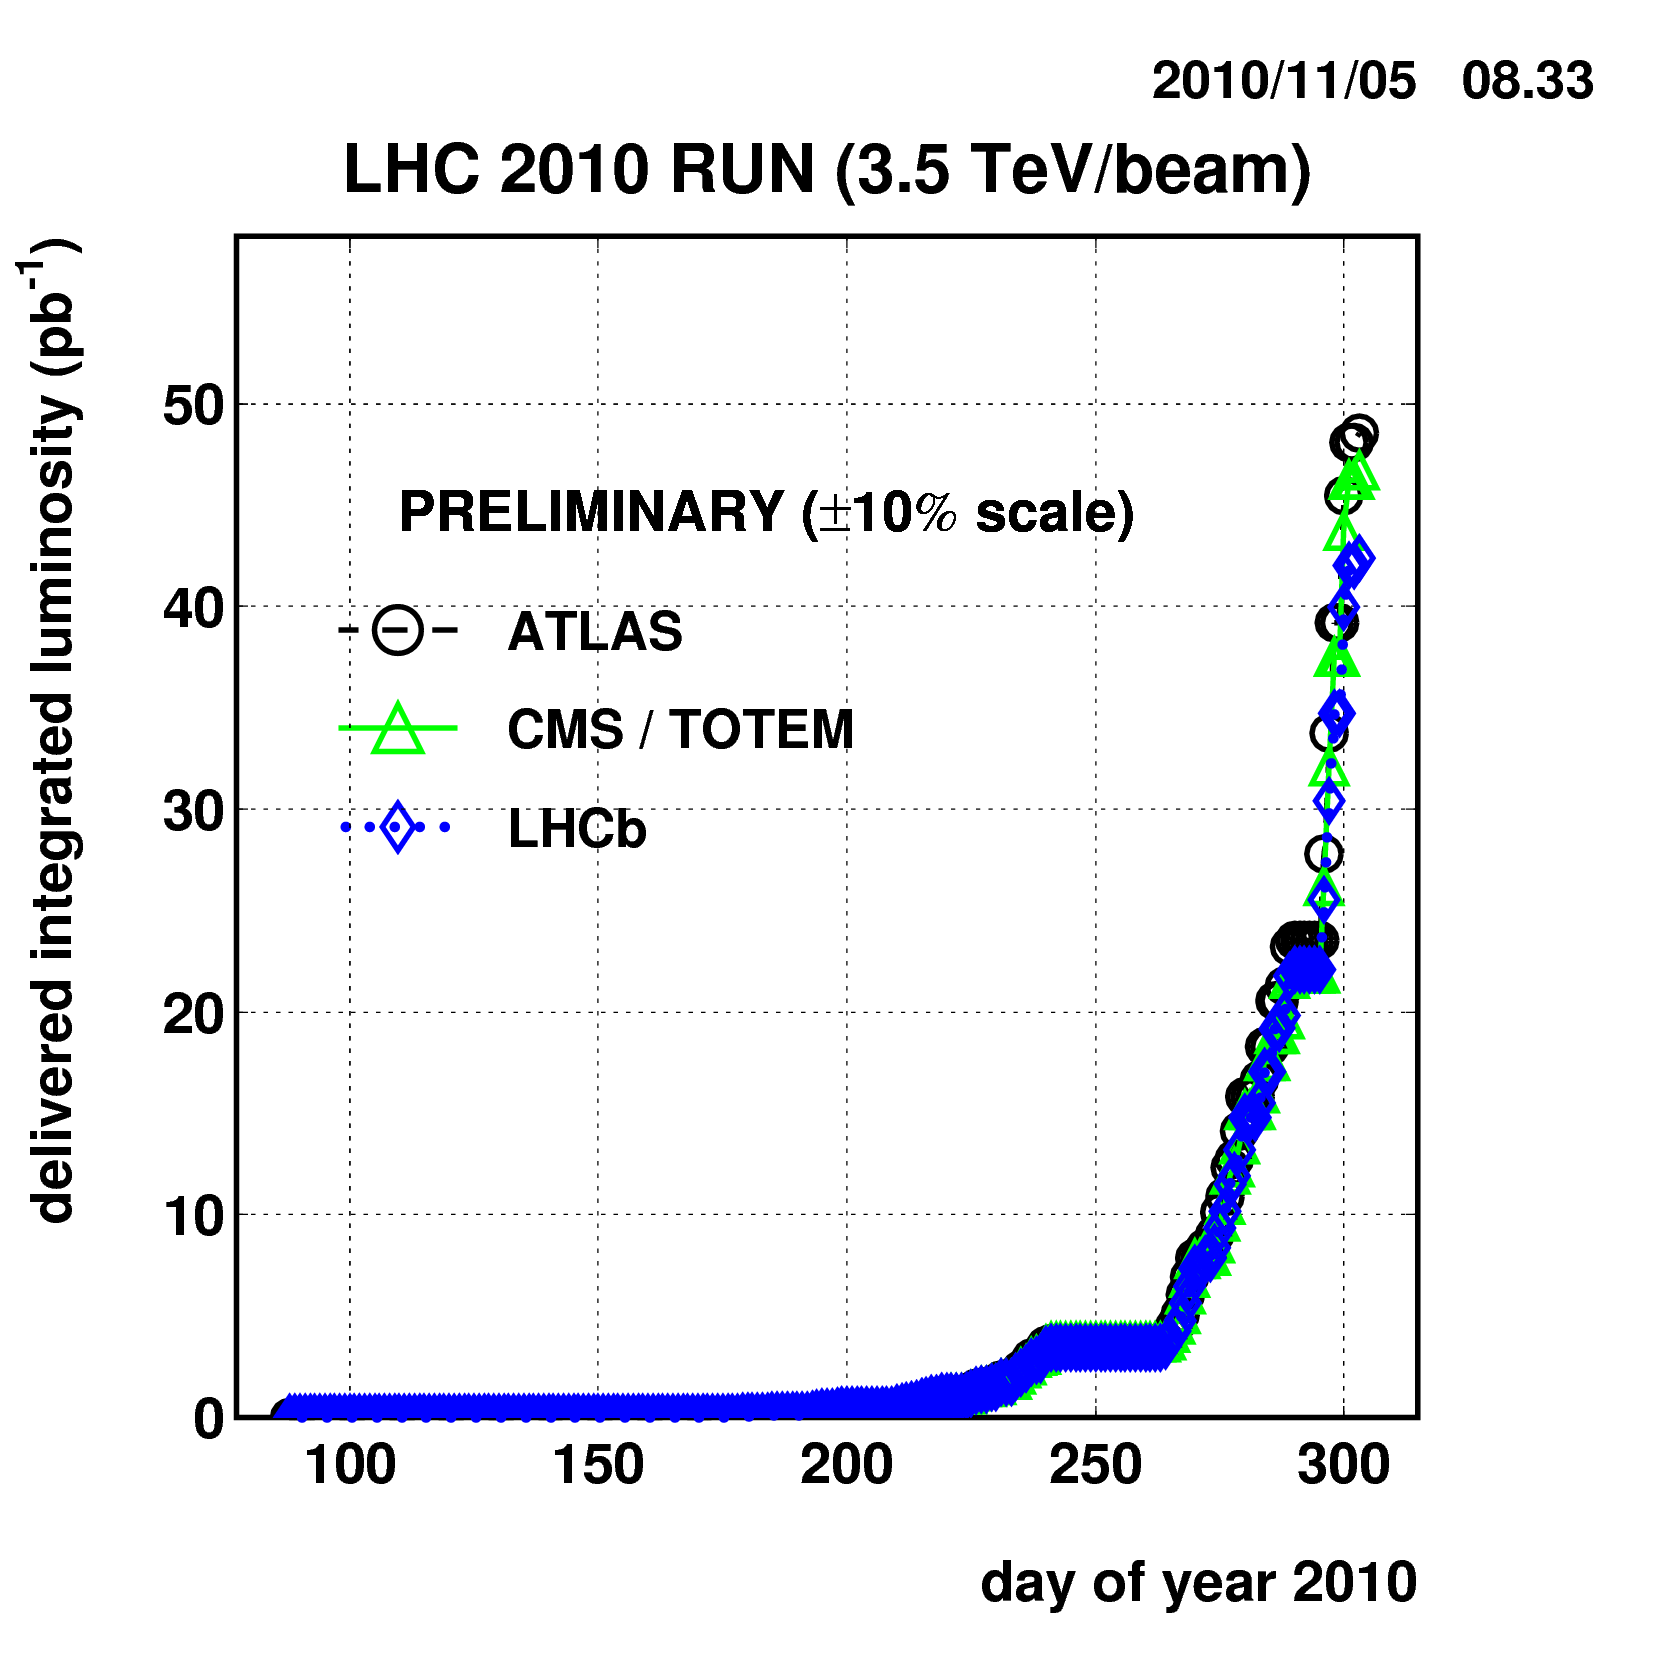
\includegraphics[width=0.49\textwidth]{Experiment/2010_lhc_luminocity.png}
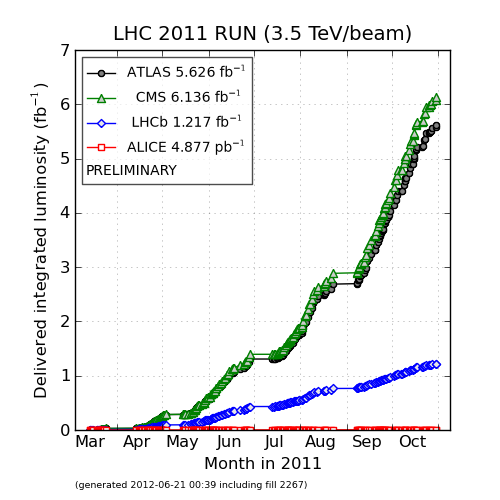
\includegraphics[width=0.49\textwidth]{Experiment/2011_lhc_luminocity.png}
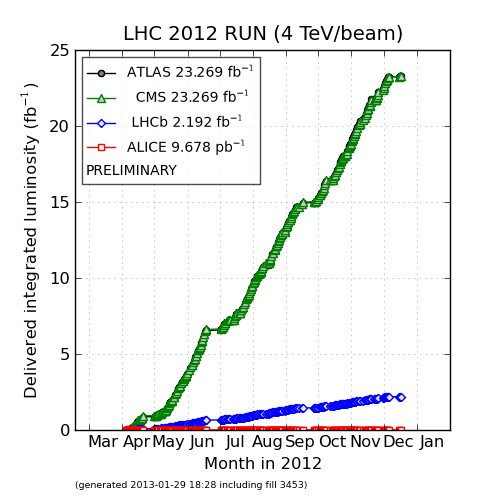
\includegraphics[width=0.49\textwidth]{Experiment/2012_lhc_luminocity.png}
\caption{Integrated luminosity delivered by the LHC to each experiment in 2010 to 2012.~\cite{lhc_lumi_plots}}
\label{fig:lhc_luminocity}
\end{figure}



%http://lpc.web.cern.ch/lpc/   %These are the LHC luminocity plots


%\subsection{Subsection heading}

%\subsubsection{Subsubsection heading}


\section{The Compact Muon Solenoid}

As one of the two general purpose detectors at the LHC, the Compact Muon Solenoid (CMS) has a wide range of physics goals, with it's main focus on the Higgs boson search. Also important are physics beyond the Standard Model, precision measurement of known physics processes, and more.  With these goals in mind, there are a number of requirements that a detector must have that are present in the CMS detector~\cite{Bayatian:922757}. These are summarized below:

\begin{itemize}
 \item
   High efficiency in muon, electron, and photon identification with excellent momentum resolution in the pseudo-rapidity region $|\eta| <$ 2.5.
 \item 
   Mass Resolution of approximately 1\% for di-muon, di-electron, and di-photon events.
 \item 
   The ability to determine the charge of muons and electrons.
 \item
   Charged particle momentum resolution and reconstruction efficiency in the inner tracker. 
 \item
   Ability to identify the primary and secondary vertices for offline tagging b-jet and $\tau$.
 \item
  $\pi_0$ rejection and efficient photon and lepton isolation.
 \item
   High performance trigger system to reduce the event rate to amounts that can be stored in real-time.
 \item
   A tracking detector with sufficient precision to limit the effects of event pile-up.
\end{itemize}


  The main parts of the CMS detector include the 3.8 T superconducting solenoid, muon system, electromagnetic calorimeter, and the tracking system \cite{CMSExperiment}.  The CMS has a number of cylindrical layers which are perpendicular to the beam axis (these are referred to as the barrel), and at both ends there are detector disks which are orthogonal to the beam axis (referred to as the end-caps). A more detailed picture of the detector can be found in Figures~\ref{fig:CMScolaborationPoster} and~\ref{fig:CMS_Slice}.  Figure~\ref{fig:CMS_luminosity} shows the collection efficiency of the CMS detector for 2010 to 2012~\cite{cms_lumi_plots}.



\begin{figure}[htb]
\centering
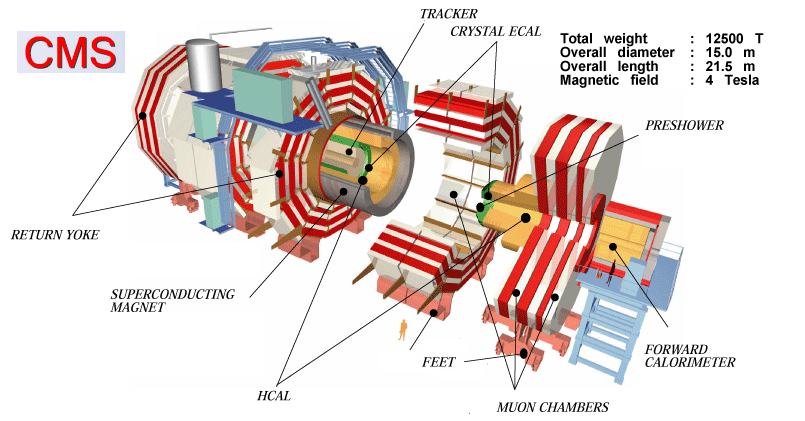
\includegraphics[width=0.99\textwidth]{Experiment/CMScollaborationPoster.png}
\caption{The CMS experiment.  HCAL stands for hadron calorimeter and ECAL stands for Electromagnetic calorimeter.}
\label{fig:CMScolaborationPoster}
\end{figure}

\begin{figure}[htb]
\centering
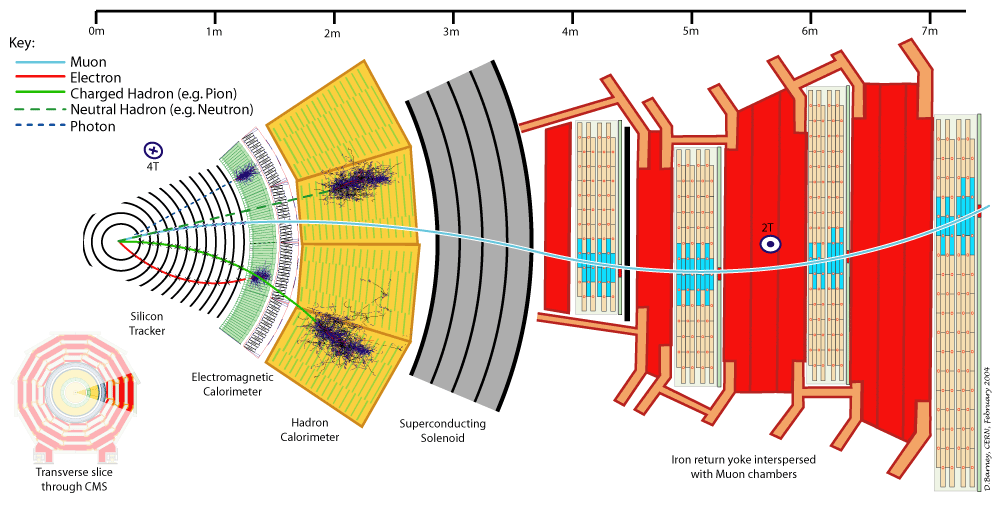
\includegraphics[width=0.99\textwidth]{Experiment/CMS_Slice.png}
\caption{A graphical slice of the CMS experiment}
\label{fig:CMS_Slice}
\end{figure}


\begin{figure}[htb]
\centering
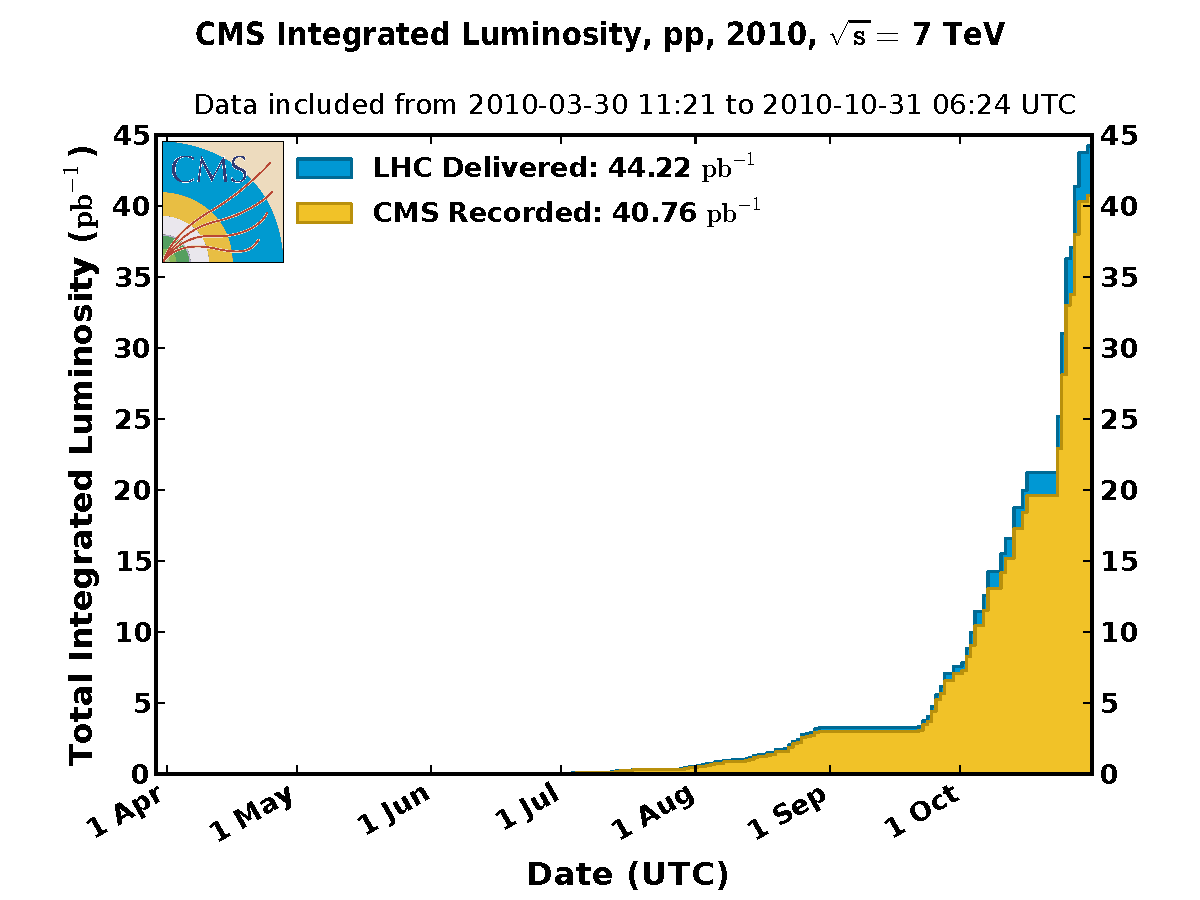
\includegraphics[width=0.49\textwidth]{Experiment/int_lumi_per_day_cumulative_pp_2010.pdf}
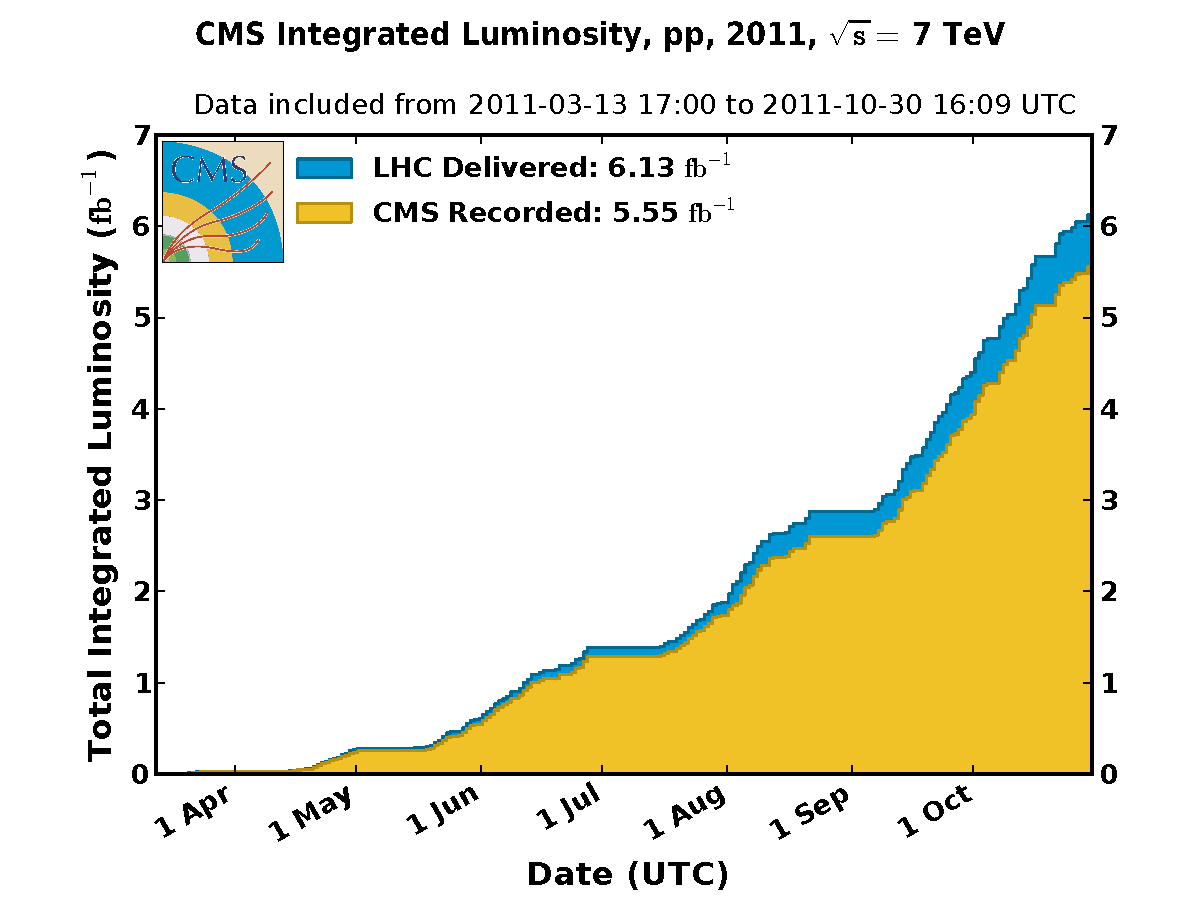
\includegraphics[width=0.49\textwidth]{Experiment/int_lumi_per_day_cumulative_pp_2011.pdf}
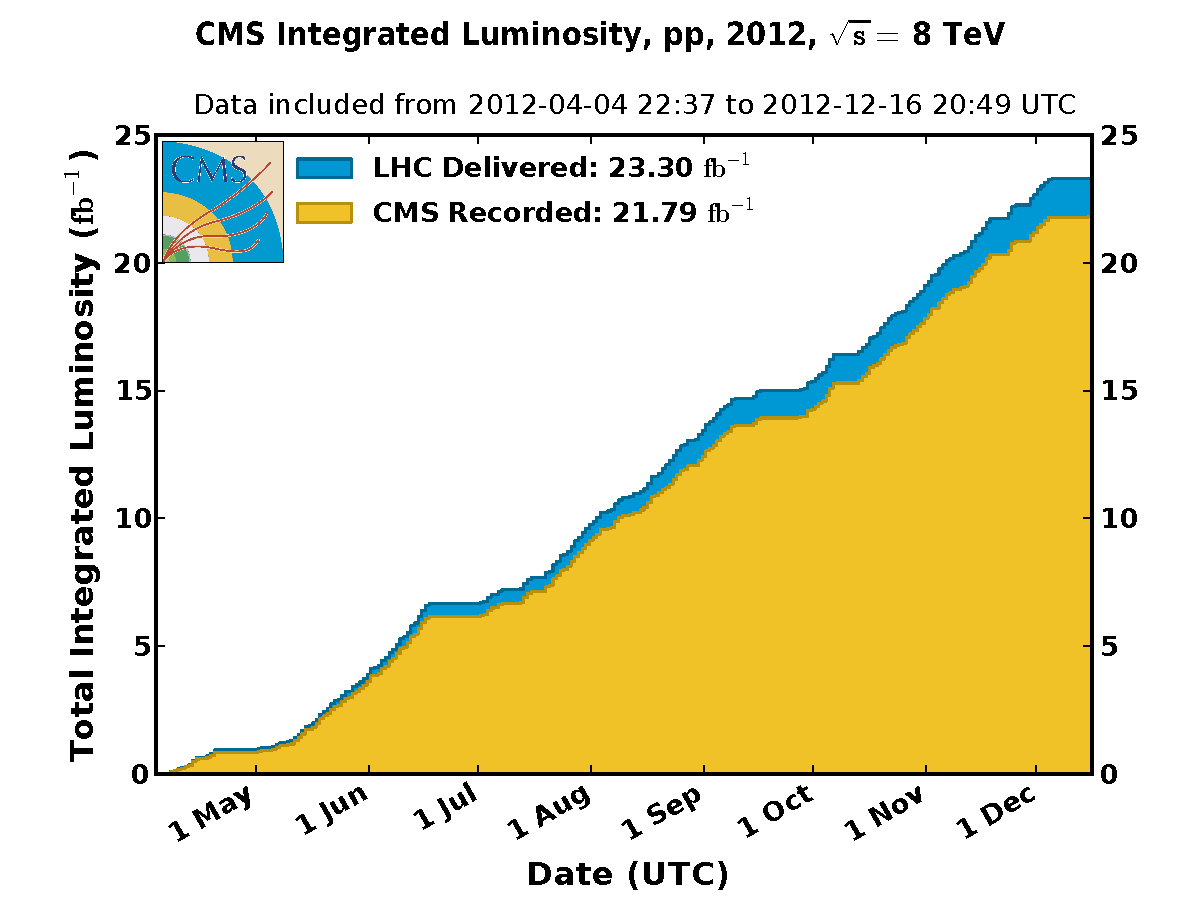
\includegraphics[width=0.49\textwidth]{Experiment/int_lumi_per_day_cumulative_pp_2012.pdf}
\caption{Total integrated luminosity for 2010 to 2012 delivered by the LHC and recorded by CMS.~\cite{cms_lumi_plots}}
\label{fig:CMS_luminosity}
\end{figure}

\subsection{CMS Subsections}
In the following sections a coordinate system will be used as illustrated in Figure~\ref{fig:CMS_detector_glossary}~\cite{Pandolfi_talk}.  Since the detector has a cylindrical shape around the beam axis the beam axis is referred to as the z axis and a cylindrical coordinate system is used.

\begin{figure}[htb]
\centering
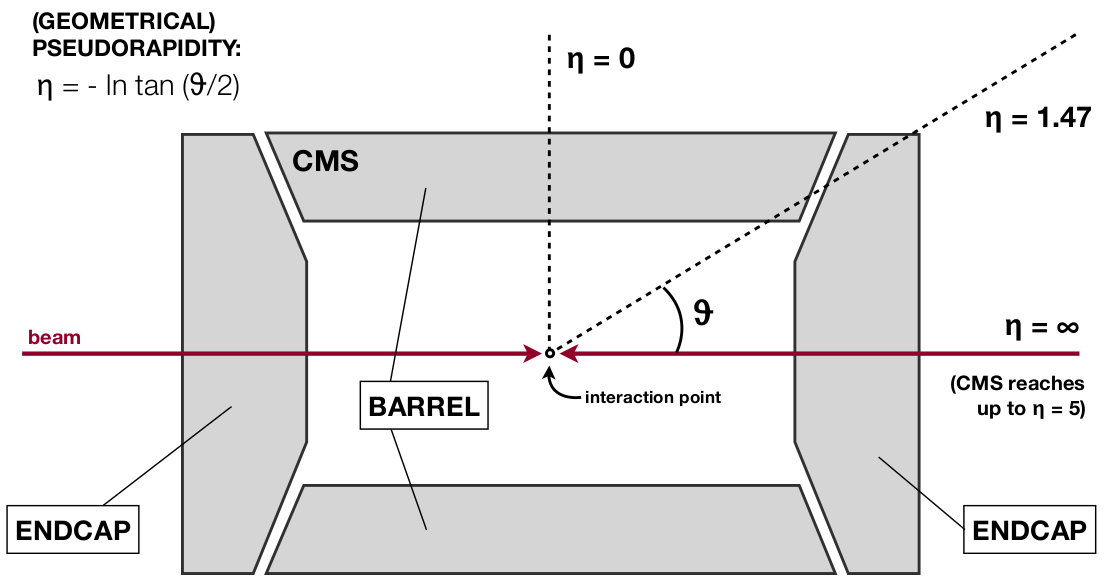
\includegraphics[width=0.99\textwidth]{Experiment/DetectorGlossary.png}
\caption{A CMS detector glossary of the cylindrical coordinate system used in this paper.~\cite{Pandolfi_talk}}
\label{fig:CMS_detector_glossary}
\end{figure}

It is useful to use the projection of momentum in the transverse plain because the net transverse momentum of collisions is close to zero.  We write:
\begin{equation} E_T = E sin \theta = \dfrac{E}{cosh\eta} \label{eq:transverse_energy}\end{equation}

When a particle is massless $E_T=p_T$.  Similarly, for the energies considered the masses are negligible and we assume that $E_T=p_T$.

\subsubsection{Magnet}

To gain the resolution needed for the muon system the bending power of the detector must be immense.  One way to archive this goal is to use a solenoid.  The magnet in CMS is a 13 m long superconducting cylindrical Niobium-Titanium coil.  This coil has a diameter of 5.9 m with a uniform magnetic field of 3.8 T at it's center.  The magnetic flux is returned by a double duty iron yoke support structure~\cite{Magnet_CMS}. This magnet can be seen in Figure~\ref{fig:CMS_solenoid_magnet}~\cite{cms_solenoid_magnet}.

\begin{figure}[htb]
\centering
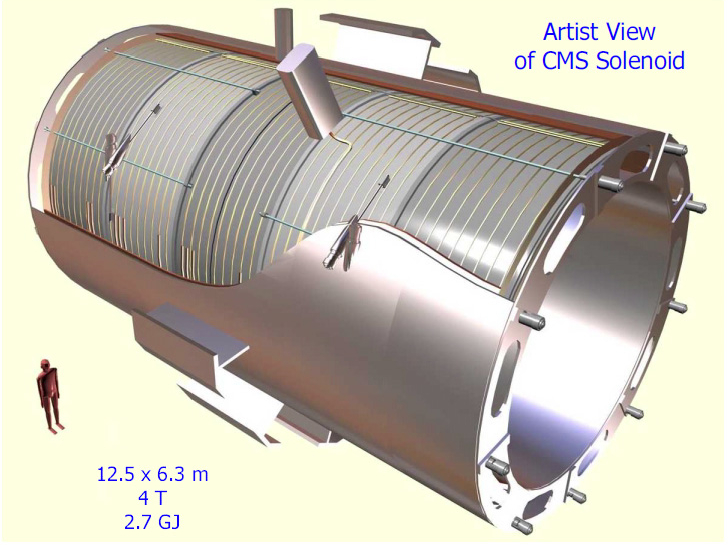
\includegraphics[width=0.59\textwidth]{Experiment/CMS-solenoid-magnet.jpg}
\caption{CMS solenoid magnet.~\cite{cms_solenoid_magnet}}
\label{fig:CMS_solenoid_magnet}
\end{figure}


\subsubsection{Tracker}
The tracker is the detector system that is closest to the primary interaction.  Its primary goal is to reconstruct the tracks of charged particles with extremely high precision both in position and momentum. The goal is greater than 95\% for electrons and muons and greater than 90\% for jets. It is also able to identify both the primary and secondary vertices.  Vertices are defined as the origin that a group of tracks share together. All these must be achieved in the extreme radioactivity that is created by the LHC collisions~\cite{cms_trakcer_project}.

The previous requirements facilitated the choice of using a large silicon tracker~\cite{cms_trakcer_project}.  The tracker has three regions that are built differently because of the change in particle flux.  The closest region is the PIXEL detector where the particle flux is at a maximum.
%is about $10^7/s$.
In the intermediate regions the flux has dropped sufficiently to be able to use silicon micro-strips.  The outer region again has lower radiation which allows larger cell size silicon micro-strips to be used.  This layout of the tracker can be seen in Figure~\ref{fig:CMS_tacker}~\cite{2010JInst...5.6007S}.

\begin{figure}[htb]
\centering
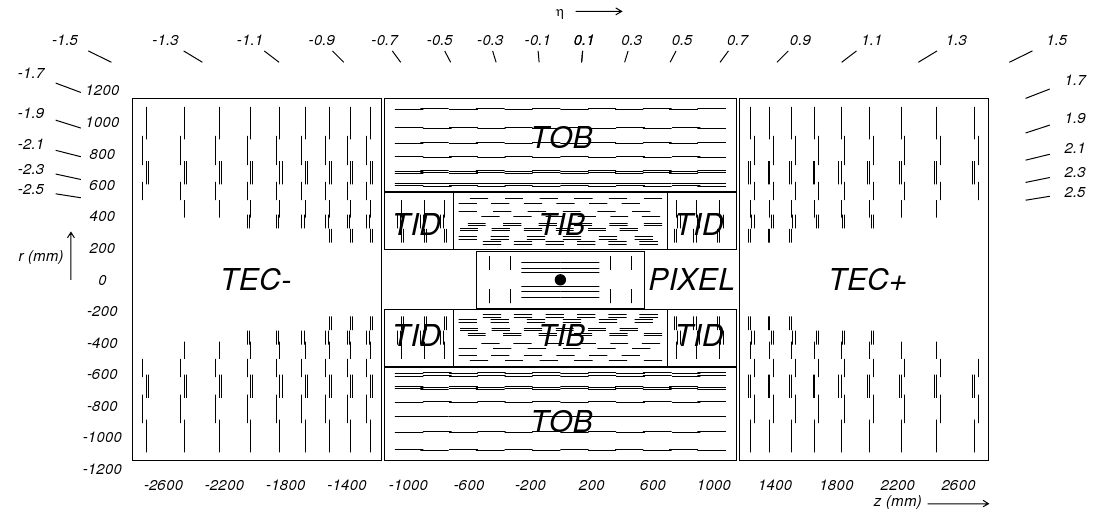
\includegraphics[width=0.69\textwidth]{Experiment/fig_cmstracker.png}
\caption{View of the CMS tracker in the rz-plane. Each line in the strip tracker represents a silicon strip detector, whereas lines in the pixel detector represent ladders and petals on which the detectors are mounted in the barrel and end-caps, respectively.~\cite{2010JInst...5.6007S}}
\label{fig:CMS_tacker}
\end{figure}

\subsubsection{The Calorimeters}

The CMS detector has two calorimeters, an electromagnetic calorimeter and a hadronic calorimeter. The electromagnetic calorimeter allows the precise measurement of both photon and electron energies.  The electromagnetic calorimeter is hermetic and homogeneous and made of 61,200 lead tungstate scintillating crystals in the barrel and 7,324 crystals in the two endcaps.~\cite{ECAL_report}

The lead tungstate crystals have a number of important features as listed below:
\begin{itemize}
  \item
    Short radiation length (0.89 cm) that allows a compact calorimeter into the small space available.
  \item
    Very fast light emission (5 ns for primary and 15 ns for secondary) since LHC bunch crossings are 25 ns.
    \item
      Radiation hard at a level to allow several years of high luminosity operation.
    \item
      Excellent position tracking because of the small shower containment. 
\end{itemize}

One downside is that the there is a low light yield so photo detectors with a high gain must be used.  Figure~\ref{fig:CMS_ecal_quadrant}~\cite{ECAL_report} shows a longitudinal cross section of the ECAL. Any dead areas where there is not detection significantly degrades the total energy measurement and hurts the missing transverse energy (MET) calculations. Figure~\ref{fig:CMS_ecal_crack} shows the gap which was designed to minimize these problems~\cite{ECAL_report}.  This area is excluded for certain measurements in the analysis for electrons in this over lap region for ($1.4442 < |\eta| < 1.566$).

\begin{figure}[htb]
\centering
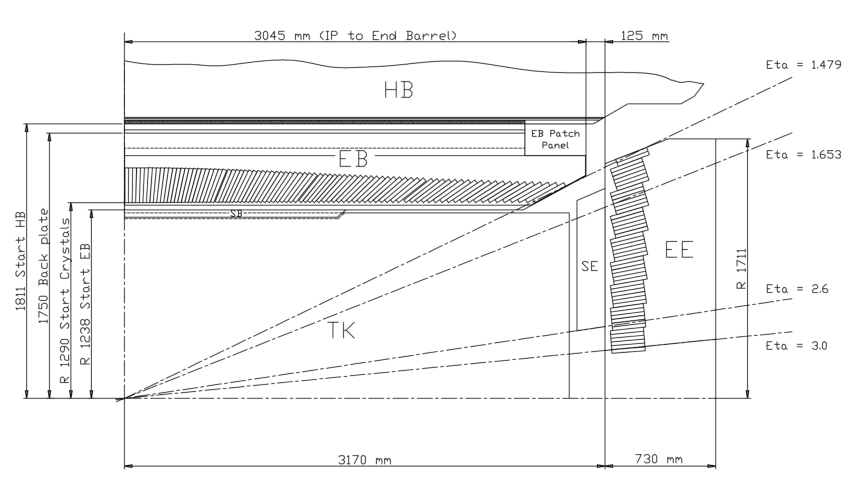
\includegraphics[width=0.69\textwidth]{Experiment/ECAL_quadrant.pdf}
\caption{Longitudinal section of the electromagnetic calorimeter (one quadrant).~\cite{ECAL_report}}
\label{fig:CMS_ecal_quadrant}
\end{figure}

\begin{figure}[htb]
\centering
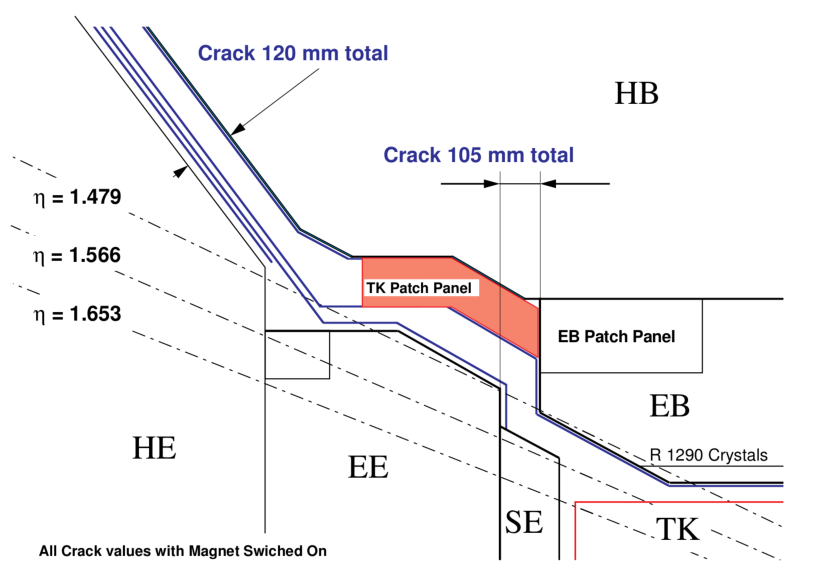
\includegraphics[width=0.69\textwidth]{Experiment/ECAL_TDR_crack.pdf}
\caption{The barrel and end-cap transition region.~\cite{ECAL_report}}
\label{fig:CMS_ecal_crack}
\end{figure}

The hadronic calorimeter~\cite{HCAL_report} detects quarks, gluons, and neutrinos.  This is done by measuring the energy and position of particle jets as well as the missing transverse energy (MET).  In conjunction with the other systems it also helps with the identification of electrons, photons, and muons with the ECAL and muon systems.  The central hadron calorimeter is a sampling calorimeter. The hadron calorimeter is made of 4mm thick plastic scintillator tiles. It uses brass as the absorber material. A quarter slice of the HCAL can be seen in Figure~\ref{fig:CMS_hcal}~\cite{Chatrchyan:2009hw}.

\begin{figure}[htb]
\centering
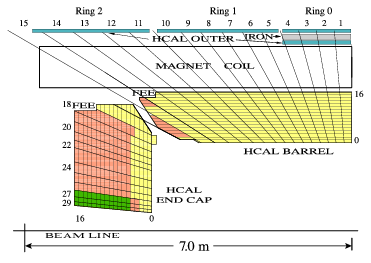
\includegraphics[width=0.69\textwidth]{Experiment/fig_HCALdiagram.png}
\caption{A quarter slice of the CMS HCAL detectors. The right end of the beam line is the interaction point. FEE denotes the location of the Front End Electronics for the barrel and the end-cap. In the diagram, the numbers on the top and left refer to segments in $\eta$, and the numbers on the right and the bottom refer to scintillator layers. Colors/shades indicate the combinations of layers that form the different depth segments, which are numbered sequentially starting at 1, moving outward from the interaction point. The outer calorimeter is assigned depth 4.~\cite{Chatrchyan:2009hw}}
\label{fig:CMS_hcal}
\end{figure}


\subsection{The CMS Trigger System}

At the high luminosity achieved at the LHC, there is the drawback that several of the interactions overlap in the same bunch crossing. Also there is overlap from different bunch crossing because of the limited speed of the detector response and data read-out.  These effects are known as pile-up.  In addition to pile-up difficulties there is an extreme amount of data produced from the collisions at CMS. With a luminosity of $10^{34}cm^{-2}s^{-1}$ there is roughly $10^9$ interactions per second.  With the typical event size of 1 MB all collisions cannot be recorded and with the majority of interactions not interesting for the CMS physics program, there needs to be a way to choose which events to record.  This is done with the triggering system to reduce the recorded rate to approximately 100 Hz. There are technical difficulties in the handling, processing, and storing of this data. These difficulties make the real time selection and recording of important events (the Trigger) very important~\cite{Bayatyan:706847}.

The CMS Trigger has two levels.  The Level 1 (L1) trigger is a hardware trigger.  The full data is stored in the pipelines for processing while waiting for the trigger decision.  If the L1 accepts the decision then the data is moved to the software based High Level Trigger (HLT).  The HLT reduces the output rate to around 100 Hz. The HLT software has a set of algorithms which give complete freedom to deciding which data to access.  To free up processing there are three virtual trigger levels.  The first only uses the muon and calorimeter data, the second adds the pixel seeds, and the final step uses the full event information.

The Level 1 Trigger is used to choose hard scattering from procecess like Higgs decays, $WW$ scattering, supersymmetry, and more.  This system is based on custom electronics.  It uses the identification of photons, electrons, muons, jets, and MET. A diagram of the L1 trigger system is shown in Figure~\ref{fig:l1triggeroverview}~\cite{Bayatyan:706847}. The physics requirements for the L1 trigger are as follows:~\cite{Bayatyan:706847}
\begin{itemize}
  \item
    The CMS trigger system should be capable of selecting leptons and jets over the pseudorapidity range $|\eta| < 2.5$, with an efficiency which is very high, above a selected threshold in transverse momentum.
  \item
    For the single lepton triggers it is required that the trigger is fully efficient ($>$ 95\%) in the pseudorapidity range $|\eta| < 2.5$, with a threshold of $p_T> 40$ GeV.
  \item
    For the dilepton trigger, it is required that the trigger is fully efficient ($>$ 95\%) in the pseudorapidity range $|\eta| < 2.5$ with thresholds of $p_T> 20$ and 15 GeV for the first and second leptons respectively.
  \item
    Single photon and diphoton triggers are required to have thresholds similar to those of the leptons.
  \item
    Single and multiple jet triggers are required with a well defined efficiency over the entire rapidity range $|\eta| < 5$ in order to reconstruct jet spectra that overlap with data attainable at lower energy colliders such as the Tevatron. For higher transverse momenta the jet trigger should also be fully efficient.
  \item
    A missing transverse energy trigger with a threshold of about 100 GeV is required.
\end{itemize}

\begin{figure}[htb]
\centering
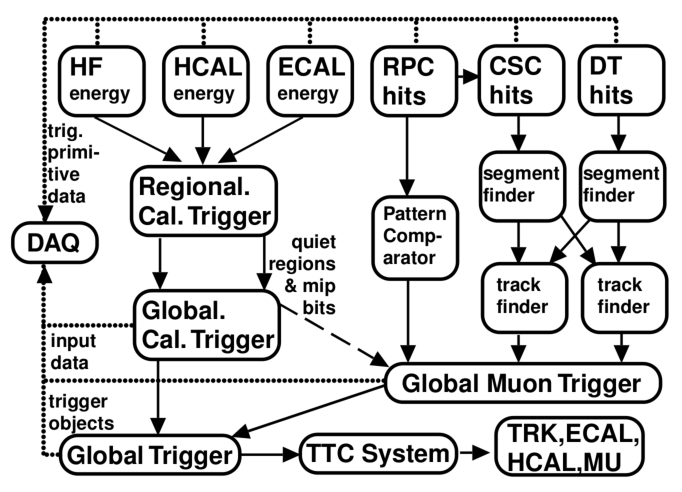
\includegraphics[width=0.69\textwidth]{Experiment/l1trigger.pdf}
\caption{Overview of Level 1 Trigger.~\cite{Bayatyan:706847}}
\label{fig:l1triggeroverview}
\end{figure}

The High-Level trigger is a software system with maximum flexability for selection and the changing enviroment of the LHC~\cite{Cittolin:578006}.  It takes the output from the Level 1 Trigger to do a rough event reconstruction.  With this rough reconstruction the HLT makes the decision to either reject the event or pass it through to a more detailed reconstruction.  This is decided by a number of criteria that are collectively used to create data sets.  These are designed to meet the various physics goals that CMS was designed to study. Common requirements are high $p_T$ lepton pairs, or large amounts of MET.%$M_T^{miss}$.



\chapter{Electron, Muon, and Jet Reconstruction}

\section{Electron Reconstruction}

Electrons are reconstructed from the tracks they form in the silicon tracker and from their energy which is deposited in the ECAL. An electron passing the silicon tracker looses energy through ionization and the emission of a photon (this process is called bremsstrahlung). This energy loss has to be taken into account.  Electron reconstruction needs to join both the tracks in the tracker and the energy deposit in the ECAL while successfully identifying the particle as an electron.  All this must happen while being careful not to identify other charged particles (like pions) as electrons. A particle incorrectly identified as an electron is called a fake electron. To take this and other problems into account, there are two different clustering algorithms that are used~\cite{Meschi:687345}. 

The energy that is collected in the calorimeter is grouped together into super-clusters. This is done along the $\phi$ direction by taking the most energetic cluster and collecting the other nearby clusters together. Once a super-cluster is created, a minimum of two hits is needed in the pixel detector in order to start the electron trajectory reconstruction. Using the trajectory, momentum, and the loose geometrical matching with the super-cluster, the tracks are matched to the appropriate super-cluster. There are four different electron classes that are corrected in different ways for bremsstrahlung and other effects.  The four types are as listed~\cite{Baffioni:934070}:

\begin{itemize}
\item
  Golden electrons. This class represents electrons least affected by radiation emission, with a reconstructed track well matching the supercluster and a well behaved supercluster pattern. 
\item
  Big Brem electrons. This class contains electrons with a good match between the energy calculated in the supercluster algorithms and the momentum recorded coming in but the supercluster does not directly match with the reconstructed track.  Also, there must be no energy loss effects from secondary photon conversion. Electrons for which all the bremsstrahlung is radiated in a single step can fall in this category.
\item
  Narrow electrons. In this intermediate class, electrons have a large bremsstrahlung fraction but not has high as Big Brem electrons.  There is a well behaved supercluster (i.e. the bremsstrahlung photons are merged inside a single cluster), but like Big Brem, it doesn't have a clean match between the tracks and the supercluster.
\item
  Showering electrons. This class contains electrons which failed to enter any of the above classes. It includes electron supercluster patterns involving one or several identified bremsstrahlung sub-cluster(s), or cases where a bad energy-momentum $E/p$ matching is observed. This is very likely in cases of secondary conversion of some early radiated bremsstrahlung for electrons having radiated a large fraction of their initial energy.
\end{itemize}

Once the electrons are corrected, the Gaussian-sum filter (GSF) algorithm for electron reconstruction is used to model the bremsstrahlung energy loss distribution by a Gaussian mixture rather than by a single Gaussian ~\cite{GSF_at_CMS}. Further cuts can be done as part of an analysis or for pre-selection to reduce fake electrons.

\section{Muon Reconstruction}

In the CMS detector muon tracks are reconstructed both in the tracker and in the muon chambers.  The muons must transverse a large amount of material before they reach the muon chambers, which lowers the resolution because of the scattering that has happened. This places a great importance on the tracker measurements both for the fine resolution and the intense magnetic field. 

First the muon tracks are reconstructed from the muon chambers. Then in a two step process these tracks from the muon chambers  are linked to the corresponding tracks found in the tracker.  First a set of tracks that match the momentum and direction of the muon chamber tracks is found.  After that a matching algorithm is applied using kinematics and angular variables to find the most accurate tracker/muon chamber track pair.
% Figure~\ref{fig:muon_pandolfi}~\cite{Pandolfi_thesis}

\begin{figure}[htb]
\centering
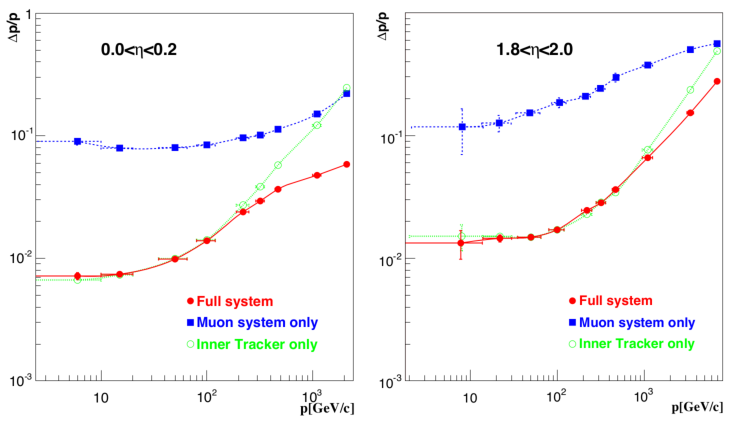
\includegraphics[width=0.69\textwidth]{Reconstruction/muon_Pandolfi.pdf}
\caption{Muon momentum resolution when using the muon spectrometers only (blue), the tracker only (green), and the full system (red): barrel ($|\eta| < $0.2) results are shown on the left, end-caps (1.8 $< |\eta| <$ 2.0) on the right.~\cite{Pandolfi_thesis}}
\label{fig:muon_pandolfi}
\end{figure}

A muon candidate made from the muon chambers and tracker information is called a global muon. If a global muon cannot be reconstructed, then using only the tracker information a tracker muon is created.  Similarly, if only a track from the muon systems is found it is reconstructed to be a stand alone muon. The High-Level Trigger uses additional criteria for a selection like isolation and momentum to create datasets for later analysis.

\section{Jet Reconstruction}

At proton colliders the reactions are primarily from the interaction of partons, which is the name given to the constituents that make up a hadron. Hadronization gives rise to columns of particles that we call jets. Jets are difficult for both theorists and experimental physicists because they are composite objects that cannot be specifically defined.  The jet reconstruction that is used is based on how particle candidates cluster using the particle flow (PF) algorithms which are described below.  This composite nature causes the detector response to vary jet to jet. This becomes a problem for the determination of the jet's energy and necessitates careful calibrations.

Light particles make up of the bulk of hadronization.  The typical breakdown of a jets energy is as follows:
\begin{itemize}
 \item
about 65\% of a jet energy is carried by charged particles, predominantly
charged pions and kaons;
\item
 20\% is converted into high-energy photons, mainly from the electromagnetic
decay of neutral mesons such as $\pi$'s and $\eta$'s;
\item
 the remaining 15\% is stored in long-lived neutral hadrons, mainly neutral
kaons, neutrons, and $\Lambda$ baryons.~\cite{Pandolfi_thesis}
\end{itemize}

With only 20\% of the jet energy being purely electromagnetic, the remaining measurements are taken through the hadronic calorimeter which leads to additional energy measurement difficulties.

The clustering of the particles that make up the jets is done with the anti-$K_t$ algorithm.  This algorithm is described in the following section. 

We first define $d_{ij}$ and $d_{iB}$~\cite{1126-6708-2008-04-063}:
\begin{equation}
d_{ij} = \min(k_{ti}^{2p}, k_{tj}^{2p}) \frac{\Delta_{ij}^2}{R^2}\,,\\
d_{iB} = k_{ti}^{2p}\,
\end{equation}

$\Delta_{ij}^2 = (y_i-y_j)^2 + (\phi_i - \phi_j)^2$ and $k_{ti}$, $y_i$ and $\phi_i$ are respectively the transverse momentum, rapidity and azimuth of particle $i$. First we find the minimum of all the distances $d_{ij}$ and $d_{iB}$. If the minimum is one of the $d_{iB}$ then it is called a jet and if it is a $d_{ij}$ we combine $i$ and $j$ into a new particle by summing over the momentum.  We continue to do this until we only have jets.

One of the benefits of this algorithm is that the distance parameter R only allows particles to be merged into jets of that specific radius or smaller.  This also results in conical jets that have radius equal to or smaller than this distance parameter. This can be seen in figure~\ref{fig:anti_atk}~\cite{1126-6708-2008-04-063}. In this analysis the R value is 0.5.

\begin{figure}

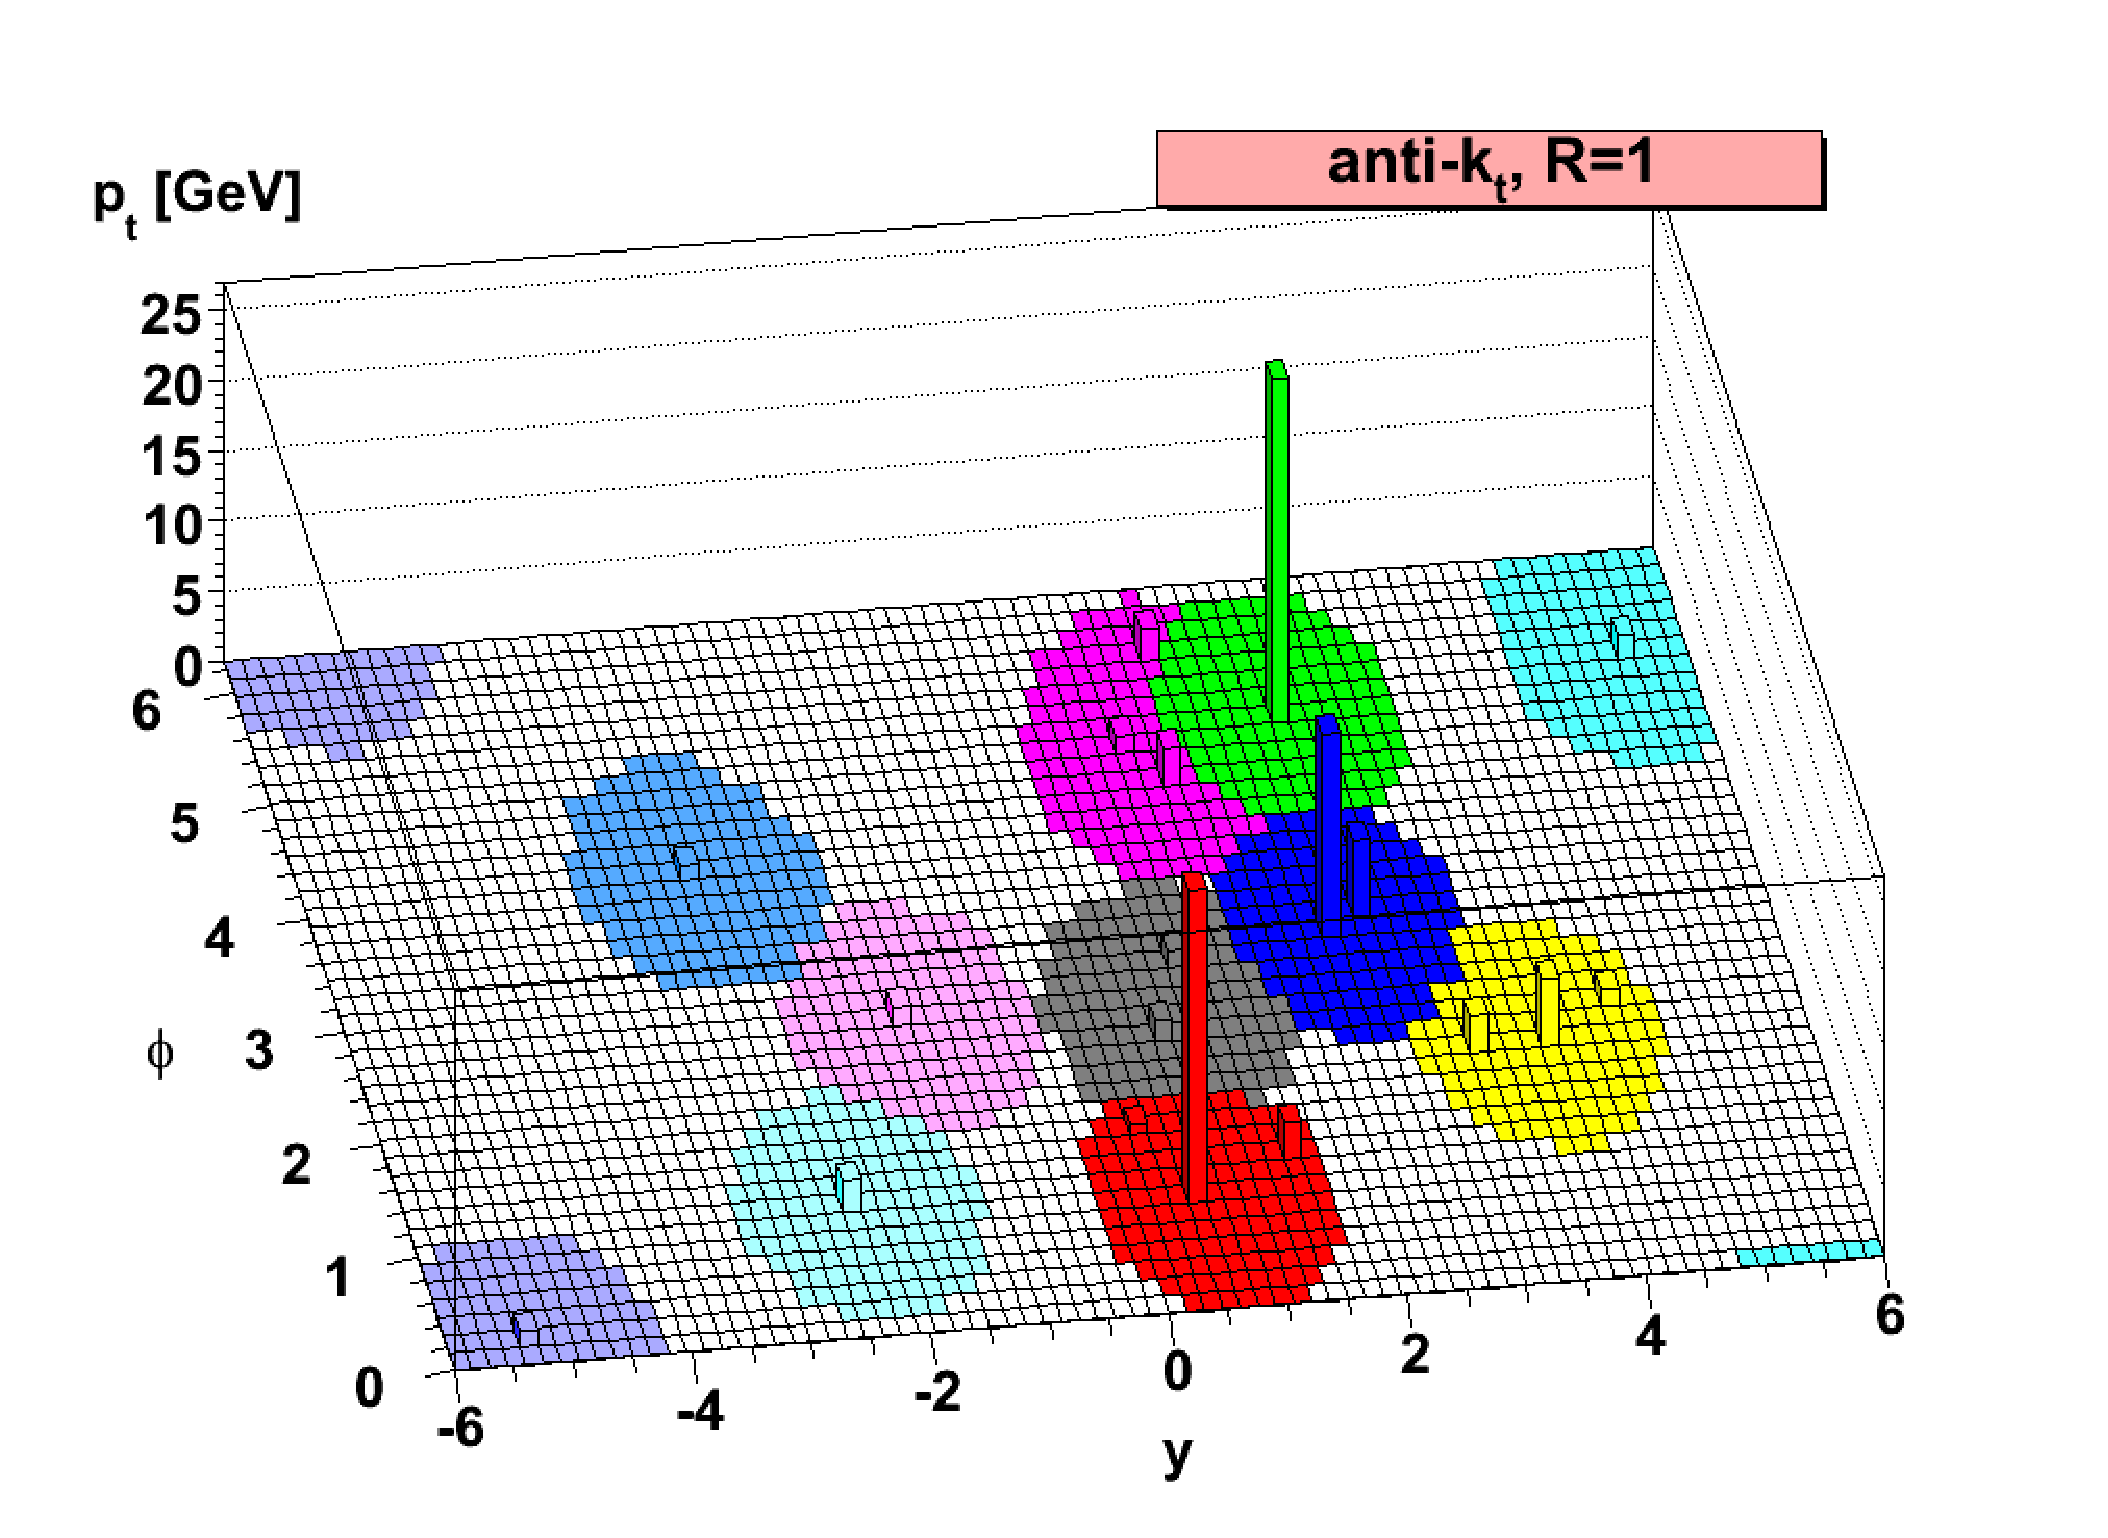
\includegraphics[width=0.79\textwidth]{Reconstruction/herwig-parton-level-ev-antikt-R1-ghosted4root.eps}
\centering
\caption{A sample parton-level event (generated with
    Herwig~\cite{Herwig}), together with many random soft ``ghosts'',
    clustered with the anti-$k_t$ algorithm, illustrating the
    ``active'' catchment areas of the resulting hard jets. This shows the cylindrical jets all with radius of R=1 or less.~\cite{1126-6708-2008-04-063}}
\label{fig:anti_atk}
\end{figure}

\section{Particle Flow Reconstruction}

At CMS particle-flow event reconstruction tries to reconstruct and identify all stable particles in the events.  This includes all the electrons, muons, charged and neutral hadrons, and photons.  It also uses information from all the sub-detectors like the tracker, both calorimeters, muon chambers, etc. After detection these particles are used as if they were Monte Carlo generated events to build the jets, MET, taus, lepton isolation, tag b-jets, and more~\cite{particleflow}.

This is possible because the CMS detector has such a large silicon tracker fully immersed in the magnetic field and the large pseudo-rapidity range. This allows particle detection for particles that have a transverse momenta as low as 150 MeV.  As previously mentioned, jet energy is only 15\% in the hadronic calorimeter. Figure~\ref{fig:jet_energy_components}~\cite{Pandolfi_thesis} shows the energy fractions as a function of pseudorapidity for the reconstruct jets on MC simulation.  


\begin{figure}
\begin{center}
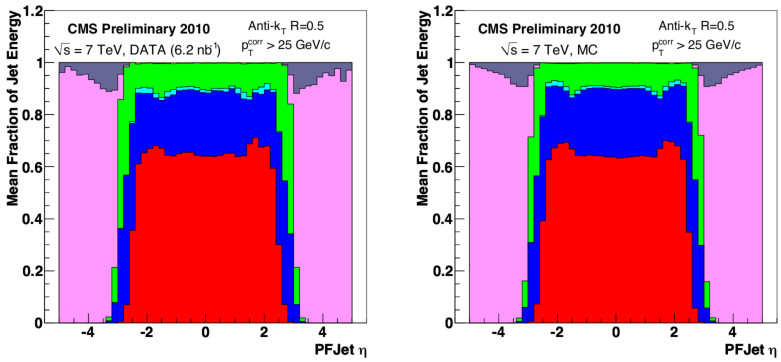
\includegraphics[width=0.99\textwidth]{Reconstruction/Pandolfi_jetenergy.pdf}
\caption{Reconstructed jet energy fractions as a function of jet pseudo-rapidity. In the central region, bottom to top: charged hadrons (red), photons (blue), electrons (cyan), neutral hadrons (green). In the forward region: HF hadrons (pink), HF electromagnetic particles (gray).~\cite{Pandolfi_thesis}}
\label{fig:jet_energy_components}
\end{center}
\end{figure}

The Particle Flow algorithm works as follows. The hits in each part of the detector are independently reconstructed and formed into blocks.  These include tracks in the tracker and calorimeter energy deposit clusters. After the blocks are formed a linking algorithm connects the ones with compatible topology to create Particle Flow Candidates (PFCandidates).  There are various types of candidates as described below~\cite{Cosa_thesis}.

\begin{itemize}
\item
Muons: a global muon, reconstructed from the combination of a track in the tracker and a track in the muon system, gives rise to a PF muon. After the identification, the corresponding track is removed from the block.
\item
 Electrons: the link between a charged-particle track and one or more ECAL clusters identifies PF electrons. The corresponding track and ECAL clusters are removed from further processing.
\item
 Charged hadrons: The remaining tracks give rise to PF charged hadrons and the momentum of the particle is taken directly from the track momentum. Tracks can be linked to ECAL and HCAL clusters if they are not identified as electrons, and the momentum is redefined taking into account information from calorimeters.
\item
Photons and Neutral hadrons: ECAL clusters not compatible with charged-tracks give rise to PF photons, while unaccounted HCAL deposits are interpreted as PF neutral hadrons.
\end{itemize}

When the full list of PFCandidates is populated, the PF Jets are reconstructed using the anti-$k_t$ algorithm as described above.  The traditional method of reconstructing jets is to use only the calorimeters.  These jets are called Calo-Jets. The difference in the jets response given by the two algorithms can be seen in figure~\ref{fig:jet_response}~\cite{particleflow}. As seen in these figures Particle Flow jets have a higher response througout the entire detector.  Further, if we look at the reconstruction between the two types of jet algorithms as a function of the transverse momentum of the jets we see an even more divergent picture.  This can be seen in figure~\ref{fig:jet_response_pt}~\cite{particleflow}. The improvement due to the Particle Flow algorithm is impressive, particularly the large improvement at the lower end of the $p_T$ spectrum.

\begin{figure}
\begin{center}
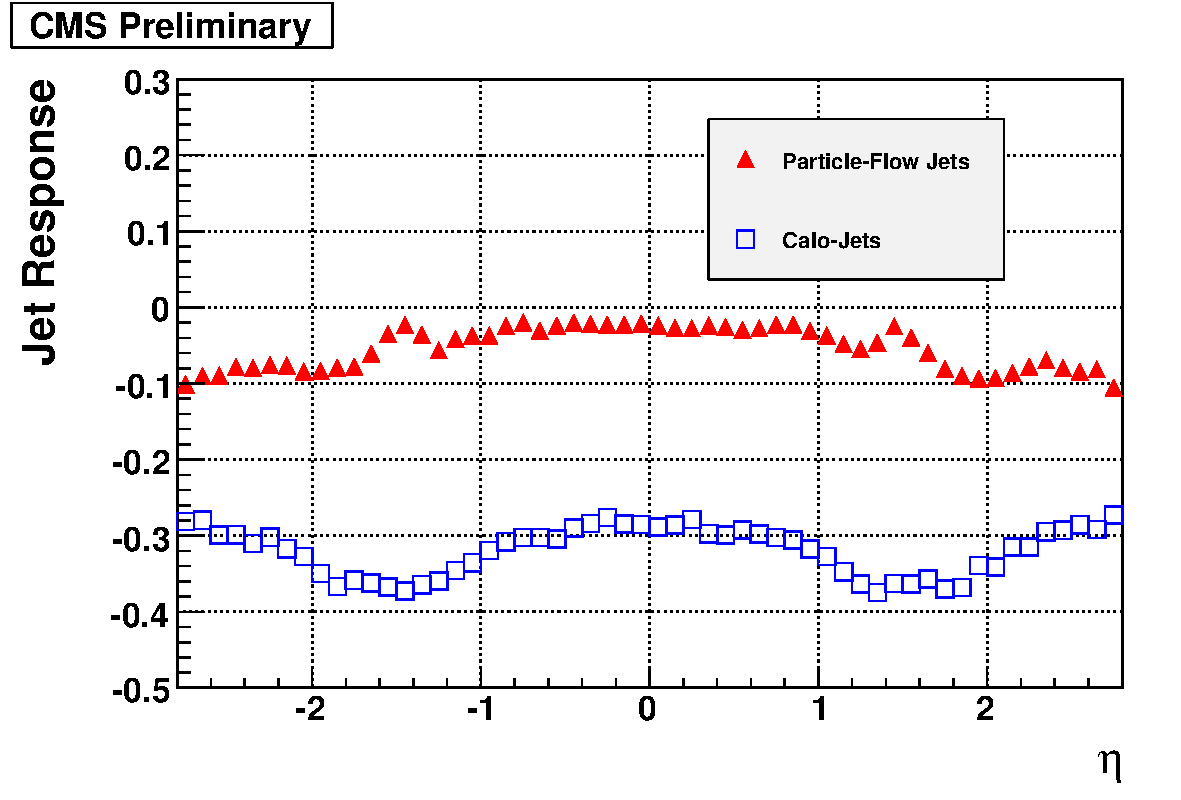
\includegraphics[width=0.79\textwidth]{Reconstruction/Figure_008-a-rotated90.pdf}\\
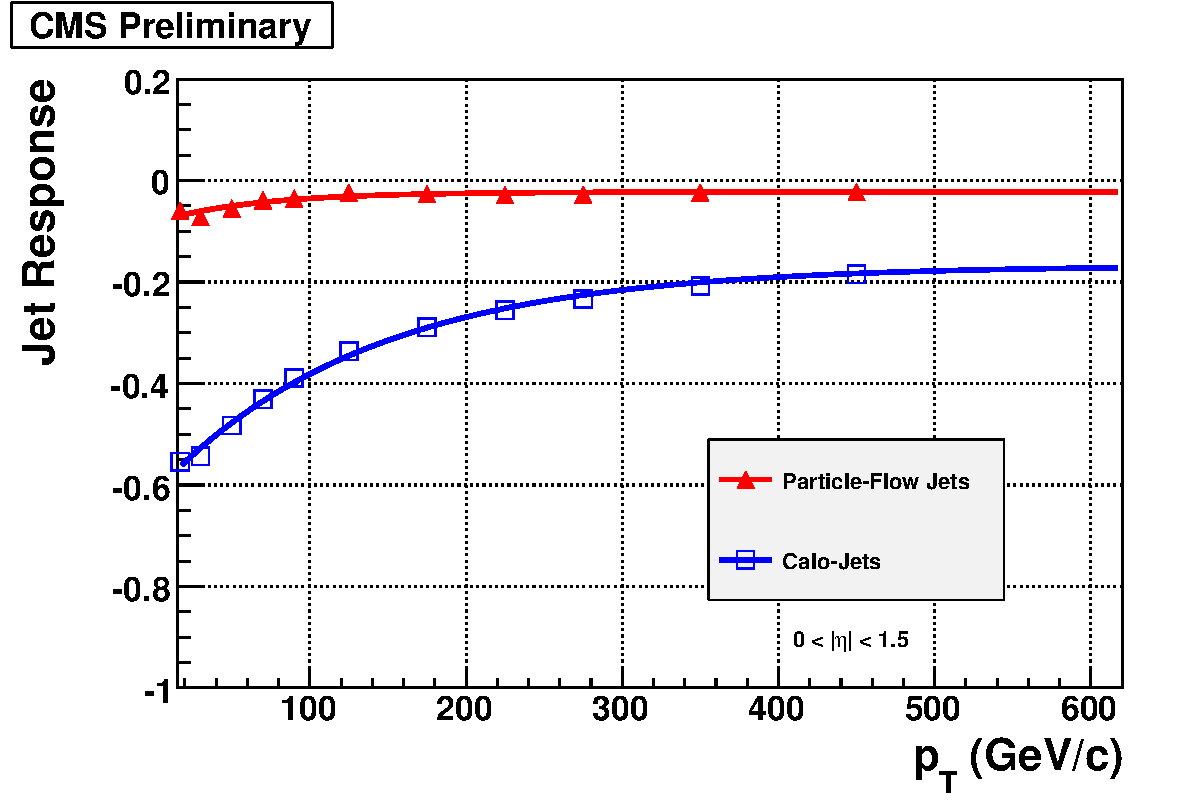
\includegraphics[width=0.49\textwidth]{Reconstruction/Figure_008-b-rotated90.pdf}
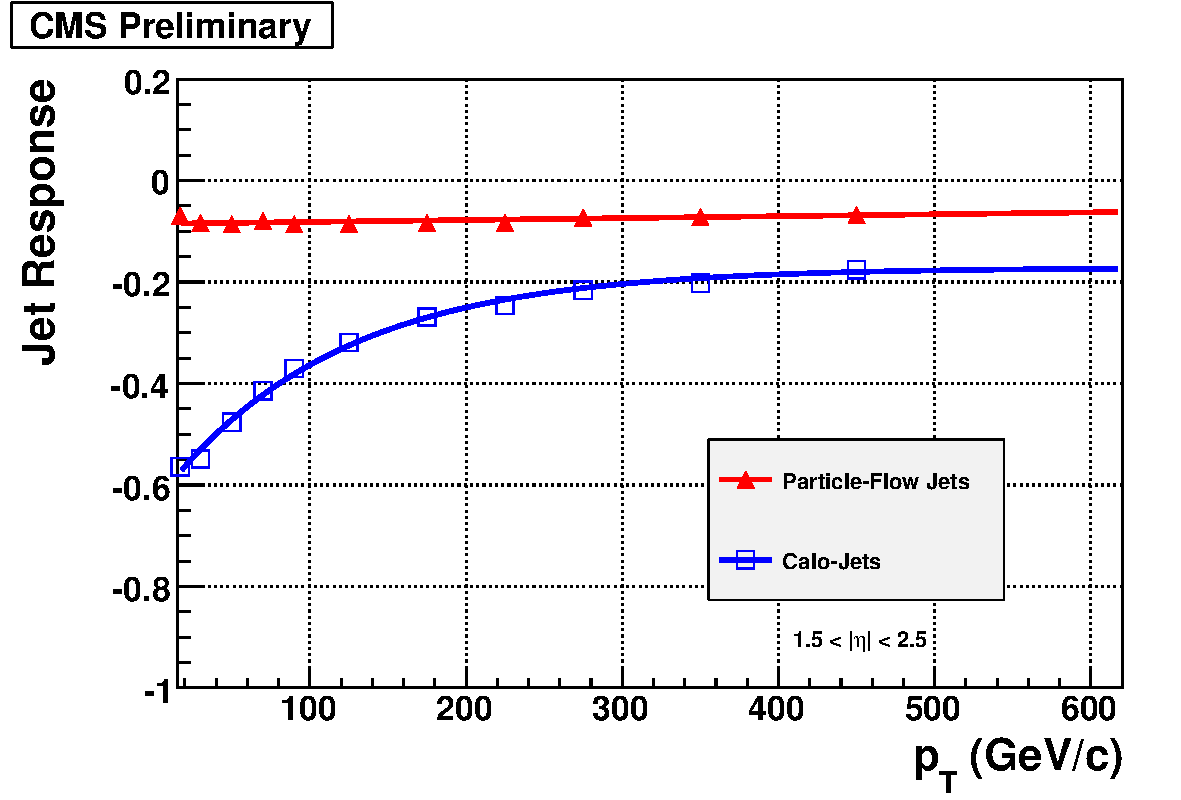
\includegraphics[width=0.49\textwidth]{Reconstruction/Figure_008-c-rotated90.pdf}
\caption{Jet response as a function of $\eta$ integrated over all $p_T$'s below 750 GeV (top) and as a function of $p_T$, in the barrel (left) and in the end-caps (right). The response curves are fit with exponential functions of $p_T$.~\cite{particleflow}}
\label{fig:jet_response}
\end{center}
\end{figure}


\begin{figure}
\begin{center}
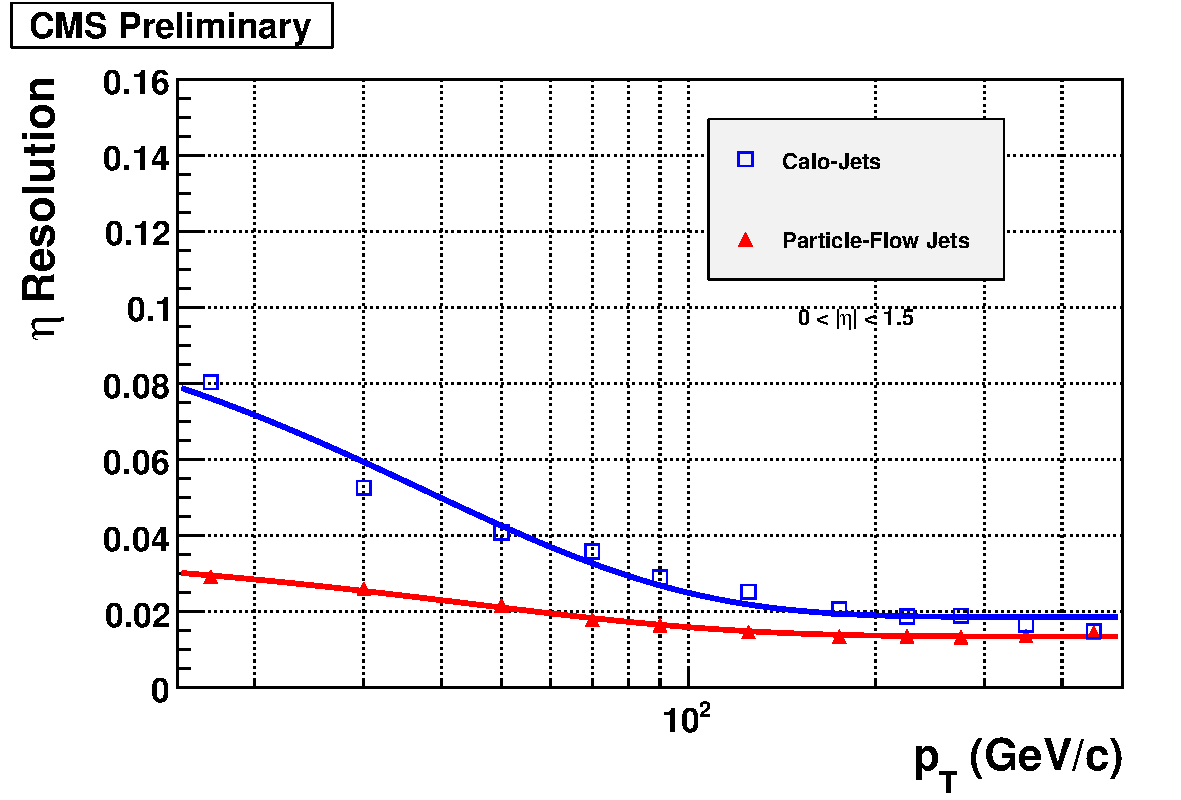
\includegraphics[width=0.49\textwidth]{Reconstruction/Figure_009-a-rotated90.pdf}
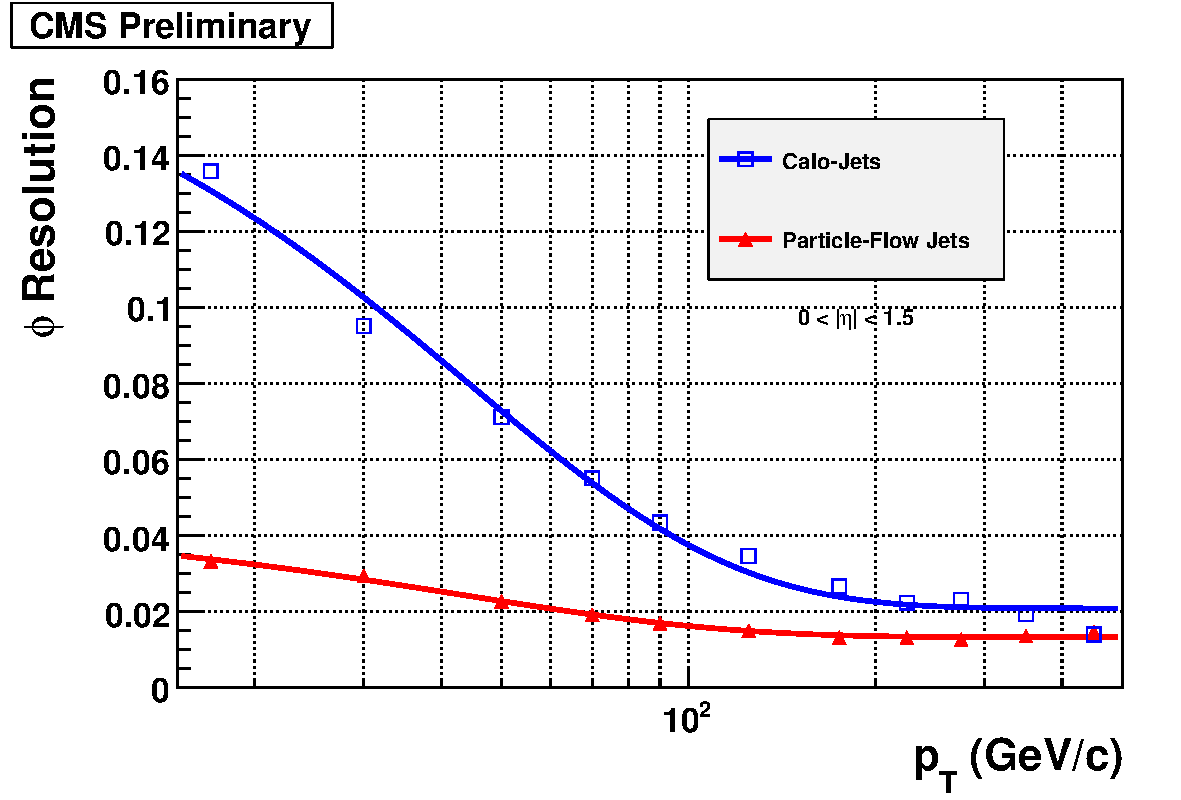
\includegraphics[width=0.49\textwidth]{Reconstruction/Figure_009-b-rotated90.pdf}
\caption{Jet-energy resolutions as a function of $p_T$ for corrected calo-jets and for particle-flow jets (upwards triangles) in the barrel (left) and in the end-caps (right). The resolution curves are fit to the sum of a constant term, a stochastic term and a noise term.~\cite{particleflow}}
\label{fig:jet_response_pt}
\end{center}
\end{figure}



%Pandolfi_jetenergy.pdf

\chapter{EVENT SELECTION}

This Chapter outlines the event selection that we use for the analysis.  A list and brief description is given of both the data and the Monte Carlo generated events. Also the cuts and motivation for the analysis preselection is given.

\section{Datasets}

The focus of this analysis is on a massive Higgs boson which is above the ZZ production threshold of 200 GeV.  Because of this high energy, the decay of one of the Z bosons will produce a pair of high $p_T$ leptons.  This will primarily fire the double-lepton HLT paths and be stored in one of the two primary datasets: DoubleElectron or DoubleMuon.  For 2012 we are using the double lepton primary datasets corresponding to 19.6 $fb^{-1}$ at 8 TeV. The data samples for 2012 are listed in Appendix~\ref{sec:tablessamples}.  Each block of data undergoes data quality monitoring (DQM) both in real-time and after the data is recorded.  Only the data recorded under good conditions for each sub-detector is certified.  Subsequently, only data that is certified as good is used in this analysis. This analysis is done on the 2012 datasets but is combined with the previous results (2011) at the end.

The data that is used in this analysis is run over centrally produced datasets that are called primary datasets.  Primary datasets are filled with events that pass the high-level triggers that are identified with that dataset.  The three primary datasets that we are concerned with are the DoubleMu, DoubleElectron, and MuEG.  The DoubleMu must have two muons that fire a specific muon HLT, DoubleElectron must fire two specific electron HLT, and MuEG must have an electron and muon that fire one of the MuEG HLTs.  More details will be given later in this chapter.



%\begin{table}[htb]
%\caption{%
%  2012 data samples.
%}
%\begin{center}
%  \begin{tabular}{ | c | c | c |} \hline
%    Channel & Dataset Name & Luminosity [$pb^{-1}$] \\ \hline \hline
%    $2\Pgm 2\Pq$ & /DoubleMu/Run2012A-13Jul2012-v1/AOD & 808 \\ 
%    & /DoubleMu/Run2012A-recover-06Aug2012-v1 & 82 \\ 
%    & /DoubleMu/Run2012B-13Jul2012-v4/AOD & 4429 \\ 
%    & /DoubleMu/Run2012C-24Aug2012-v1/AOD & 495 \\ 
%    & /DoubleMu/Run2012C-PromptReco-v2/AOD & 6394 \\ 
%    & /DoubleMu/Run2012D-PromptReco-v1/AOD & 4580 \\ \hline
    
%    $2\Pe 2\Pq$ & /DoubleElectron/Run2012A-13Jul2012-v1/AOD & 808 \\ 
%    & /DoubleElectron/Run2012A-recover-06Aug2012-v1 & 82 \\
%    & /DoubleElectron/Run2012B-13Jul2012-v4/AOD & 4429 \\ 
%    & /DoubleElectron/Run2012C-24Aug2012-v1/AOD & 495 \\ 
%    & /DoubleElectron/Run2012C-PromptReco-v2/AOD & 6394 \\ 
%    & /DoubleElectron/Run2012D-PromptReco-v1/AOD & 4580 \\ \hline

%    $\Pgm \Pe \Pq \Pq $ & /MuEG/Run2012A-13Jul2012-v1/AOD & 808 \\ 
%    & /MuEG/Run2012A-recover-06Aug2012-v1/AOD & 82 \\ 
%    & /MuEG/Run2012B-13Jul2012-v4/AOD & 4429  \\
%    & /MuEG/Run2012C-24Aug2012-v1/AOD & 495  \\ 
%    & /MuEG/Run2012C-EcalRecover 11Dec2012-v1/AOD & 134  \\
%    & /MuEG/Run2012C-PromptReco-v2/AOD & 6394 \\
%    & /MuEG/Run2012D-PromptReco-v1/AOD & 7274 \\ \hline
    %\multicolumn{2}{|c|}{Photon purity cuts} \\ \hline
%  \end{tabular}
%\end{center}
%\label{tab:2012datasamples}
%\end{table}




\subsection{Simulated Events}

Monte Carlo (MC) simulations are useful for studying the properties of the SM Higgs boson and the backgrounds that are relevant to this analysis.  The dominant background in this analysis is the inclusive Z production with jets. Particularly those jets coming from b-quarks.  The Z+Jets sample uses the MADGRAPH generator~\cite{MadGraph07}. MADGRAPH is a Next-to-Leading-Order (NLO) matrix element generator.  Other backgrounds are $\Pqt \Paqt$, ZZ, WW and WZ.  The main portion of the top background is from $\Pqt \Paqt \rightarrow 2l2\nu 2b$ and the sample for this is generated using POWHEG~\cite{Powheg04,Powheg07,Powheg08} which is interfaced with PYTHIA 6~\cite{pythia} to do the final parton showering and hadronization.  For ZZ, WZ, and WW, they are fully generated with PYTHIA 6.  The Monte Carlo samples for these processes are listed in Appendix~\ref{sec:tablessamples}. 

The signal Monte Carlo samples used in this analysis were generated using POWHEG and vary for $M_H$ from 230 $GeV/c^2$ up to 1000 $GeV/c^2$.  These samples can also be seen in Appendix~\ref{sec:tablessamples}.  Each sample has 3$\times 10^{-5}$ events. The cross-sections multiplied by the branching ratio for $H \rightarrow ZZ \rightarrow 2l2q$ are listed as well.  The $H \rightarrow ZZ$ branching fraction is provided as a function of the Higgs boson mass by the LHC Higgs cross section working group~\cite{LHCHiggsCrossSectionWorkingGroup:2011ti,LHCHiggsCrossSectionWorkingGroup:2012ti}. The branching ratios of $Z \rightarrow \Plp \Plm$ and $Z \rightarrow \Pq \Paq$ are from the Particle Data Group (PDG)~\cite{pdg}. These numbers can be found in Appendix~\ref{sec:tablessamples}.

%\begin{table}[htb]
%\caption{%
%  2012 background MC samples.
%}
%\footnotesize
%\begin{center}
%  \begin{tabular}{ | c | c | c | c |} \hline
%    Process & Dataset Name &  $\sigma$ [pb] &  Luminosity [$fb^{-1}$] \\ \hline \hline
%    Z+jets (inclusive) & DYJetsToLL\_M-50\_TuneZ2Star\_8TeV-madgraph	& 3503.71 & 8.7 \\ 
%    & & & \\
%    
%    Z+1 jet (exclusive) & DY1JetsToLL\_M-50\_TuneZ2Star\_8TeV-madgraph	& 660.6 & 36.4 \\ 
%    Z+2 jet (exclusive) & DY2JetsToLL\_M-50\_TuneZ2Star\_8TeV-madgraph	& 215.1 & 101.6 \\ 
%    Z+3 jet (exclusive) & DY3JetsToLL\_M-50\_TuneZ2Star\_8TeV-madgraph	& 65.79 & 167.4 \\ 
%    Z+4 jet (exclusive) & DY4JetsToLL\_M-50\_TuneZ2Star\_8TeV-madgraph	& 27.59 & 232.1 \\
%    & & & \\
%    $\Pqt \Paqt$ & TTJets\_TuneZ2star\_8TeV-madgraph-tauola	& 23.38 & 461 \\ 
%    WW & WW\_TuneZ2star\_8TeV\_pythia6\_tauola	&	57.1097 & 168 \\ 
%    WZ & WZ\_TuneZ2star\_8TeV\_pythia6\_tauola	&	22.88 & 424  \\ 
%    ZZ & ZZ\_TuneZ2star\_8TeV\_pythia6\_tauola	&	17.654 & 549 \\ \hline
%    %\multicolumn{2}{|c|}{Photon purity cuts} \\ \hline
%  \end{tabular}
%\end{center}
%\label{tab:2012backmcsamples}
%\end{table}
%\normalsize


%%%%%%%%%%%%%%%%%%%%%%%%%%%%%%%%%%%%%%%%%%%%%%%%%
%\begin{table}[htb]
%\caption{
%POWHEG signal MC samples $H \rightarrow ZZ \rightarrow 2l2q, \,\,\,\, l = e, \mu, \tau$ 2012.
%}
%\label{tab:2012sigmcsamples}
%\vspace*{\medskipamount}
%\begin{center}
%\scriptsize
%\begin{tabular}{|c|l|c|}
%\hline
%$M_H$ (GeV) & Name & $\sigma(H \rightarrow 2l2q)$ [pb]  \\ \hline \hline
%200 & /GluGluToHToZZTo2L2Q\_M-200\_8TeV-powheg-pythia6/ & 0.2566 \\ & Summer12-PU\_S7\_START52\_V9-v1/AODSIM &  \\ \hline
%210 & /GluGluToHToZZTo2L2Q\_M-210\_8TeV-powheg-pythia6/ & 0.2538 \\ & Summer12-PU\_S7\_START52\_V9-v1/AODSIM &  \\ \hline
%220 & /GluGluToHToZZTo2L2Q\_M-220\_8TeV-powheg-pythia6/ & 0.2416 \\ & Summer12-PU\_S7\_START52\_V9-v1/AODSIM &  \\ \hline
%230 & /GluGluToHToZZTo2L2Q\_M-230\_8TeV-powheg-pythia6/ & 0.2278 \\ & Summer12-PU\_S7\_START52\_V9-v1/AODSIM &  \\ \hline
%250 & /GluGluToHToZZTo2L2Q\_M-250\_8TeV-powheg-pythia6/ & 0.2022 \\ & Summer12-PU\_S7\_START52\_V9-v1/AODSIM &  \\ \hline
%275 & /GluGluToHToZZTo2L2Q\_M-275\_8TeV-powheg-pythia6/ & 0.1751 \\ & Summer12-PU\_S7\_START52\_V9-v1/AODSIM &  \\ \hline
%300 & /GluGluToHToZZTo2L2Q\_M-300\_8TeV-powheg-pythia6/ & 0.1563 \\ & Summer12-PU\_S7\_START52\_V9-v1/AODSIM &   \\ \hline
%325 & /GluGluToHToZZTo2L2Q\_M-325\_8TeV-powheg-pythia6/ &  0.1478 \\ & Summer12-PU\_S7\_START52\_V9-v1/AODSIM &   \\ \hline
%350 & /GluGluToHToZZTo2L2Q\_M-350\_8TeV-powheg-pythia6/ & 0.1482 \\  & Summer12-PU\_S7\_START52\_V9-v1/AODSIM &   \\ \hline
%375 & /GluGluToHToZZTo2L2Q\_M-375\_8TeV-powheg-pythia6/ & 0.1360 \\     & Summer12-PU\_S7\_START52\_V9-v1/AODSIM &   \\ \hline
%400 & /GluGluToHToZZTo2L2Q\_M-400\_8TeV-powheg-pythia6/ &  0.1111 \\    & Summer12-PU\_S7\_START52\_V9-v1/AODSIM &   \\ \hline
%425 & /GluGluToHToZZTo2L2Q\_M-425\_8TeV-powheg-pythia6/ & 0.0914 \\    & Summer12-PU\_S7\_START52\_V9-v1/AODSIM &  \\ \hline
%450 & /GluGluToHToZZTo2L2Q\_M-450\_8TeV-powheg-pythia6/ & 0.7311 \\    & Summer12-PU\_S7\_START52\_V9-v1/AODSIM &  \\ \hline
%475 & /GluGluToHToZZTo2L2Q\_M-475\_8TeV-powheg-pythia6/ & 0.6 \\    & Summer12-PU\_S7\_START52\_V9-v1/AODSIM &  \\ \hline
%500 & /GluGluToHToZZTo2L2Q\_M-500\_8TeV-powheg-pythia6/ & 0.4719 \\    & Summer12-PU\_S7\_START52\_V9-v1/AODSIM &  \\ \hline
%525 & /GluGluToHToZZTo2L2Q\_M-525\_8TeV-powheg-pythia6/ & 0.0380 \\    & Summer12-PU\_S7\_START52\_V9-v1/AODSIM &  \\ \hline
%550 & /GluGluToHToZZTo2L2Q\_M-550\_8TeV-powheg-pythia6/ & 0.0305 \\    & Summer12-PU\_S7\_START52\_V9-v1/AODSIM &  \\ \hline
%575 & /GluGluToHToZZTo2L2Q\_M-575\_8TeV-powheg-pythia6/ & 0.025 \\    & Summer12-PU\_S7\_START52\_V9-v1/AODSIM &  \\ \hline
%600 & /GluGluToHToZZTo2L2Q\_M-600\_8TeV-powheg-pythia6/ &  0.0201 \\    & Summer12-PU\_S7\_START52\_V9-v1/AODSIM &  \\ \hline
%\end{tabular}
%\end{center}
%\end{table}


\section{Pile-Up}


In the extreme intensities at the LHC, many pp interactions overlap each other.  These extra interactions are known as pile-up with respect to the interaction of interest. When simulations are generated, the pile-up conditions of the detector are one of the input parameters, but these conditions can change and produce a mismatch between Monte Carlo and data.  To correct this, we use scale factors to re-weight the simulated events in both the muon and electron channels~\cite{cms_lumi_plots}.  The 2012 distributions and their corrections can be seen in Figure~\ref{fig:PileUp}. All following sections have the pile-up re-weighting applied to all simulated samples.  

\begin{figure}[htb]
\centering
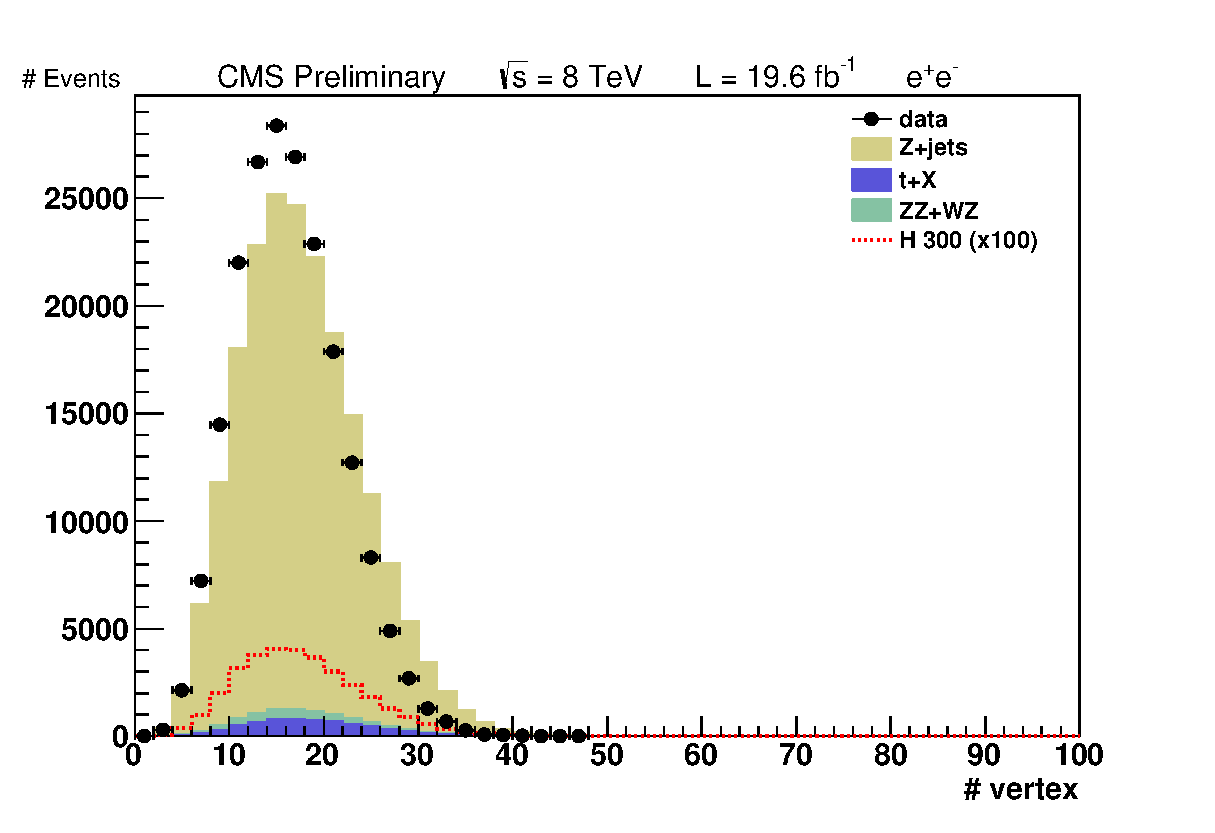
\includegraphics[width=0.49\textwidth]{Selection/before_el_nvtx.eps}
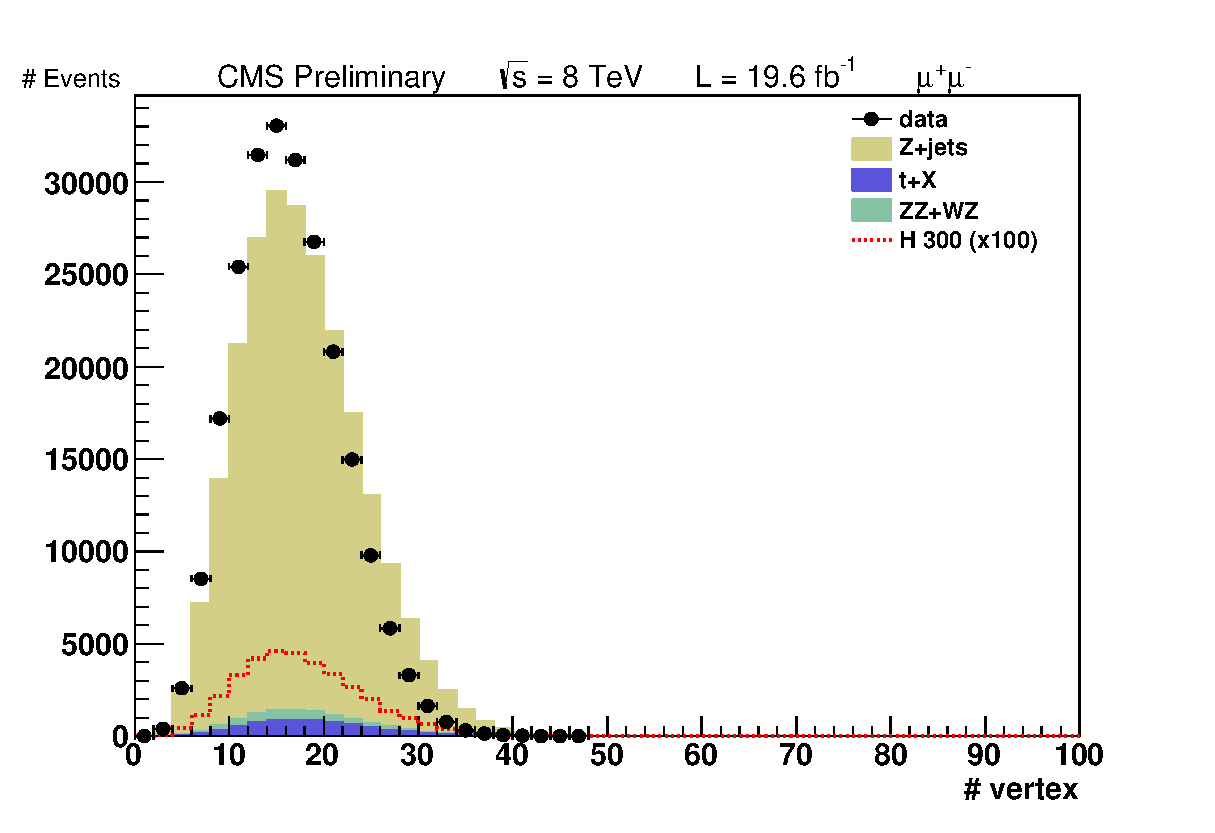
\includegraphics[width=0.49\textwidth]{Selection/before_mu_nvtx.eps}\\
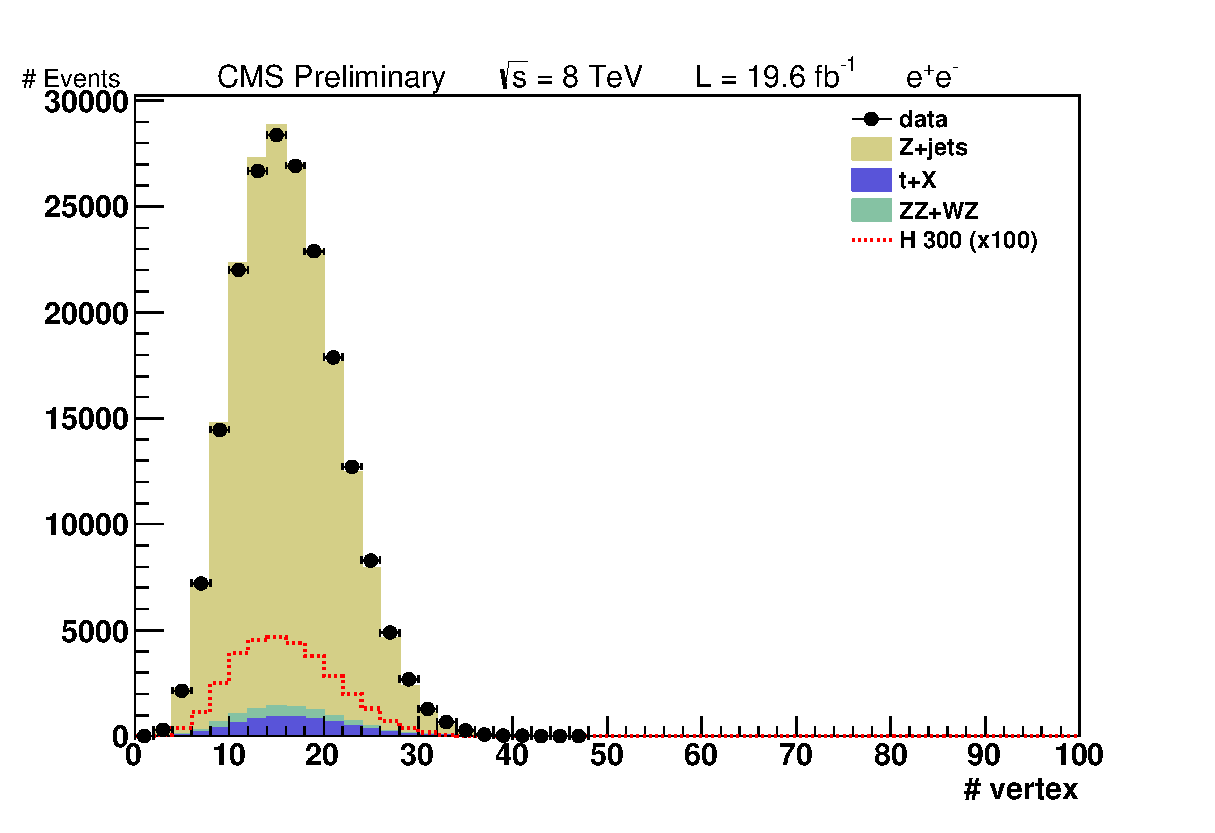
\includegraphics[width=0.49\textwidth]{Selection/after_el_nvtx.eps}
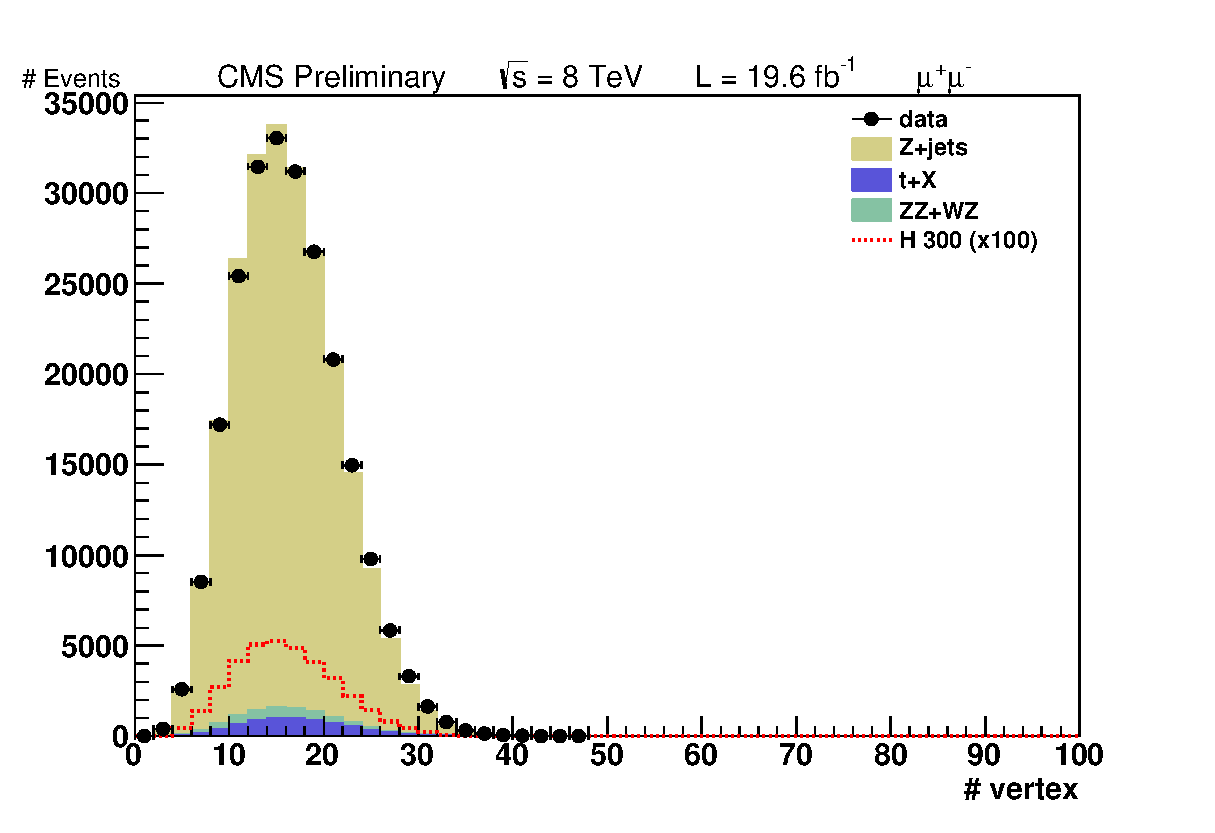
\includegraphics[width=0.49\textwidth]{Selection/after_mu_nvtx.eps}\\
\caption{Top Left: Number of interaction in the 2012 data and the simulated samples for electrons.  Top Right:  Number of interaction in the 2012 data and the simulated samples for muons. Bottom Left: Electron Monte Carlo pile-up corrected. Bottom Right: Muon Monte Carlo pile-up corrected.}
\label{fig:PileUp}
\end{figure}


%after_mu_nvtx.eps



\section{Preselection}
The Higgs boson signal events we are searching for have a signature of a lepton pair and a quark pair.  Both pairs will have an invariant mass that peaks around the Z boson mass.  $M_{lljj}$ is the invariant mass of the $\Plp \Plm \Pq \Paq$ system which corresponds to the hypothetical Higgs boson mass.  This is the main discriminating variable that we have to differentiate signal from background.

As mentioned above, particles are reconstructed from the measured detector interactions using the particle flow algorithm. We analyze events in the DoubleMu and DoubleElectron datasets. In each of these datasets, there is at least one un-prescaled trigger with looser requirements than the off-line selections. Only events which satisfy the lowest threshold un-prescaled trigger for the dataset are considered for the analysis. The trigger requirements are summarized in Table~\ref{triggers}.% More details on the trigger strategies for Higgs searches are available in~\cite{hlt}.

For muons in 2011, the {\tt HLT\_DoubleMu7} HLT was used and required that there were two muon candidates reconstructed at the HLT level.  Both of these had to have a transverse momentum larger than 7 GeV. As the luminosity of the LHC increased, this HLT was prescaled (only a fraction of the events passing were recorded) and we began to use {\tt HLT\_Mu13\_Mu8}.  This required the transverse momentum of one of the muons to be 13 GeV or larger and the other to be 8 GeV or larger.  Again this trigger was then prescaled because of increasing luminosity and the {\tt HLT\_Mu17\_Mu8} trigger was used for the final parts of 2011. Also the SingleMu dataset was added with the {\tt HLT\_IsoMu24} trigger to give a complete picture of the events. In 2012 only the {\tt HLT\_Mu17\_Mu8} trigger on the DoubleMuon dataset was used requiring one muon to have a transverse momentum above 17 GeV and another muon with transverse momentum above 8 GeV.  

Similar to the muon, HLT electrons are required to have one transverse momentum above 17 GeV and another electron with transverse momentum above 8 GeV.  In addition to this, there are a number of other requirements on isolation to reduce the number of fake electrons.

%%%%%%%%%%%%%%%%%%%%%%%%%%%%%%%%%%%%%%%%%%%%%%%%%
\begin{table*}[htb!]
\caption{ 
Event trigger requirements for data.
}
\label{triggers}
\vspace*{\medskipamount}
\begin{center}
\small
\begin{tabular}{|l l|}
\hline
\bf{Dataset} & \bf{2011 trigger requirement}   \\
\hline
DoubleMu & \tt{HLT\_DoubleMu7} \\
 & \tt{HLT\_Mu13\_Mu8} \\
 & \tt{HLT\_Mu17\_Mu8} \\ \hline
SingleMu & \tt{HLT\_IsoMu24} \\ \hline
DoubleElectron & \tt{HLT\_Ele17\_CaloIdL\_CaloIsoVL\_Ele8\_} \\ 
& \tt{CaloIdL\_CaloIsoVL} \\
 & \tt{HLT\_Ele17\_CaloIdT\_TrkIdVL\_CaloIsoVL\_TrkIsoVL\_} \\
 & \tt{Ele8\_CaloIdT\_TrkIdVL\_CaloIsoVL\_TrkIsoVL} \\ \hline
\bf{} & \bf{2012 trigger requirement}   \\
\hline
DoubleMu & \tt{HLT\_Mu17\_Mu8}\\
 & \tt{HLT\_Mu17\_TkMu8} \\ \hline
DoubleElectron & \tt{HLT\_Ele17\_CaloIdT\_TrkIdVL\_CaloIsoVL\_TrkIsoVL\_} \\ 
& \tt{Ele8\_CaloIdT\_TrkIdVL\_CaloIsoVL\_TrkIsoVL} \\
\hline
\end{tabular}
\end{center}
\end{table*}
%%%%%%%%%%%%%%%%%%%%%%%%%%%%%%%%%%%%%%%%%%%%%%%%%
Since the level of precision of the trigger emulation in simulation is not well known, no trigger is applied on MC samples. Instead, proper event weights are assigned to MC events according to the probabilities of lepton candidates to pass the trigger. The trigger efficiency tables for leptons satisfying the same identification criteria as in the analysis are computed in bins of ($pt$, $\eta$) from data using tag \& probe techniques~\cite{CMS-AN-2011-399}. 

\subsection{Lepton Selection}
$Z \rightarrow \Pem \Pep$ and $Z \rightarrow \Pgmm \Pgmp$ candidates are constructed from pairs of same-flavor, opposite-charge lepton candidates, which satisfy kinematic and identification criteria. Electron candidates are reconstructed with the GSF algorithm and in order to assure good electron reconstruction a cut is applied: the $\eta$ of the electron super-cluster must be inside the ECAL acceptance volume ($|\eta|<2.5$) but outside the ECAL barrel-endcap overlap region ($1.4442<|\eta|<1.566$). Muon candidates must have been reconstructed by both the GlobalMuon and the PF muon reconstruction algorithms and must satisfy the acceptance cut $|\eta|<2.4$.

Electron candidates must satisfy the standard ``Loose'' working point of the cut-based electron identification for 2012 analysis. The cuts are listed in Appendix~\ref{sec:datamcsf} and comprise proper electron identification requirements, an isolation cut, and conversion rejection criteria. Muon candidates must satisfy the standard ``Tight'' working point of the cut-based muon ID for 2012 analysis. The cuts are listed in Appendix~\ref{sec:datamcsf} and comprise proper muon identification requirements plus an isolation cut.

%%%%%%%%%%%%%%%%%%%%%%%%%%%%%%%%%%%%%%%%%%%%%%%%%
%\begin{table*}[htb]
%\caption{ 
%Electron ID requirements for the Loose ID working point.
%}
%\label{tab:electronid}
%\vspace*{\medskipamount}
%\begin{center}
%\small
%\begin{tabular}{|l|l|l|}
%\hline
%Variable & Barrel cut & Endcap cut  \\
%\hline
%$\Delta \eta_{trk, supercluster}$ & $<0.007$ & $<0.009$ \\
%$\Delta \phi_{trk, supercluster}$ & $<0.15$ & $<0.1$ \\
%$\sigma_{i\eta, i\eta}$ & $<0.01$ & $<0.03$ \\
%$H/E$ & $<0.12$ & $<0.10$ \\
%$d_{0}$ (wrt primary vertex) & $< 0.2 mm$ & $< 0.2 mm$ \\
%$d_z$ (wrt primary vertex) & $< 2 mm$ & $< 2 mm$ \\
%$|1/E - 1/p|$ & $< 0.05$ & $<0.05$ \\
%$I_{PF, \,\, corr}/p_T$ & $< 0.15$ & $<0.15$ \\
%Missing hits & $\le 1$ & $\le 1$ \\
%Conversion vertex fit prob.& $< 10^{-6}$ & $< 10^{-6}$ \\
%\hline
%\end{tabular}
%\end{center}
%\end{table*}
%%%%%%%%%%%%%%%%%%%%%%%%%%%%%%%%%%%%%%%%%%%%%%%%%
Given a lepton candidate, the PF isolation is defined as the sum of deposits (i.e. $p_T$ or $E_T$) of charged hadrons ($I_{ch}$), neutral hadrons ($I_{nh}$), and photons ($I_{ph}$), computed in a $\Delta R$ cone around the lepton direction. In order to assure independence of the isolation from the number of PU interactions, a corrected PF isolation definition is used as follows: 
\begin{equation} I_{PF, \,\, corr} = I_{ch}(PFnoPU) + max(I_{nh}+I_{ph}- \rho \cdot A_{eff} , 0) \end{equation}

In the above corrected definition, only deposits from charged hadrons not coming from PU vertexes ($I_{ch}(PFnoPU)$) are considered.  From these we subtract an overall PU energy contribution which is estimated as the average energy density in the event ($\rho$) multiplied by an effective area $A_{eff}$. This is strictly following the recommendations of egamma and muon POGs (Physics Object Group). The POGs are special groups within the CMS collaboration that define optimal methods of working with physics objects. The isolation cone for electrons is defined as $\Delta R < 0.3$, while for muons is defined as $\Delta R < 0.4$. The proper $A_{eff}$ values are provided by the POGs in bins of lepton $\eta$. A cut is applied on the relative PF isolation ($I_{PF, \,\, corr} / p_T$) as reported in Appendix~\ref{sec:datamcsf}.
%%%%%%%%%%%%%%%%%%%%%%%%%%%%%%%%
%\begin{table*}[htb!]
%\caption{ 
%Muon ID requirements for the Tight ID working point.
%}
%\label{tab:muonid}
%\vspace*{\medskipamount}
%\begin{center}
%\small
%\begin{tabular}{|l|l|}
%\hline
%Variable & Cut  \\
%\hline
%isGlobalMuon & True \\
%isPFMuon & True \\
%$\chi^2 / ndof$ (global fit) & $<10$ \\
%Muon chamber hits in global fit & $>0$ \\
%Muon stations with muon segments & $>1$ \\
%$d_{xy}$ (from tracker, wrt primary vertex) & $< 2 mm$  \\
%$d_z$ (from tracker, wrt primary vertex) & $< 5 mm$  \\
%Valid pixel hits (tracker track) & $> 0$ \\
%Tracker layers with hits & $>5$ \\
%$I_{PF, \,\, corr}/p_T$ & $< 0.12$ \\
%\hline
%\end{tabular}
%\end{center}
%\end{table*}
%%%%%%%%%%%%%%%%%%%%%%%%%%%%%%%%%%%%%%%%%%%%%%%%%




$Z \rightarrow ee $ and $Z \rightarrow \mu\mu$ candidates are constructed from pairs of opposite-charge leptons. The leading lepton of the pair must have $p_T > 40 GeV$,
while the next-to-leading lepton must have $p_T > 20 GeV$. The invariant mass of the pair must be $ 70 < m_{\ell \ell} < 110 GeV $. The di-lepton invariant mass for the selected $Z \rightarrow \ell \ell$ candidates is shown in Fig.~\ref{fig:m_dilepton}.  
%%%%%%%%%%%%%%%%%%%%%%%
\begin{figure}[htb!]
\begin{center}
\centerline{
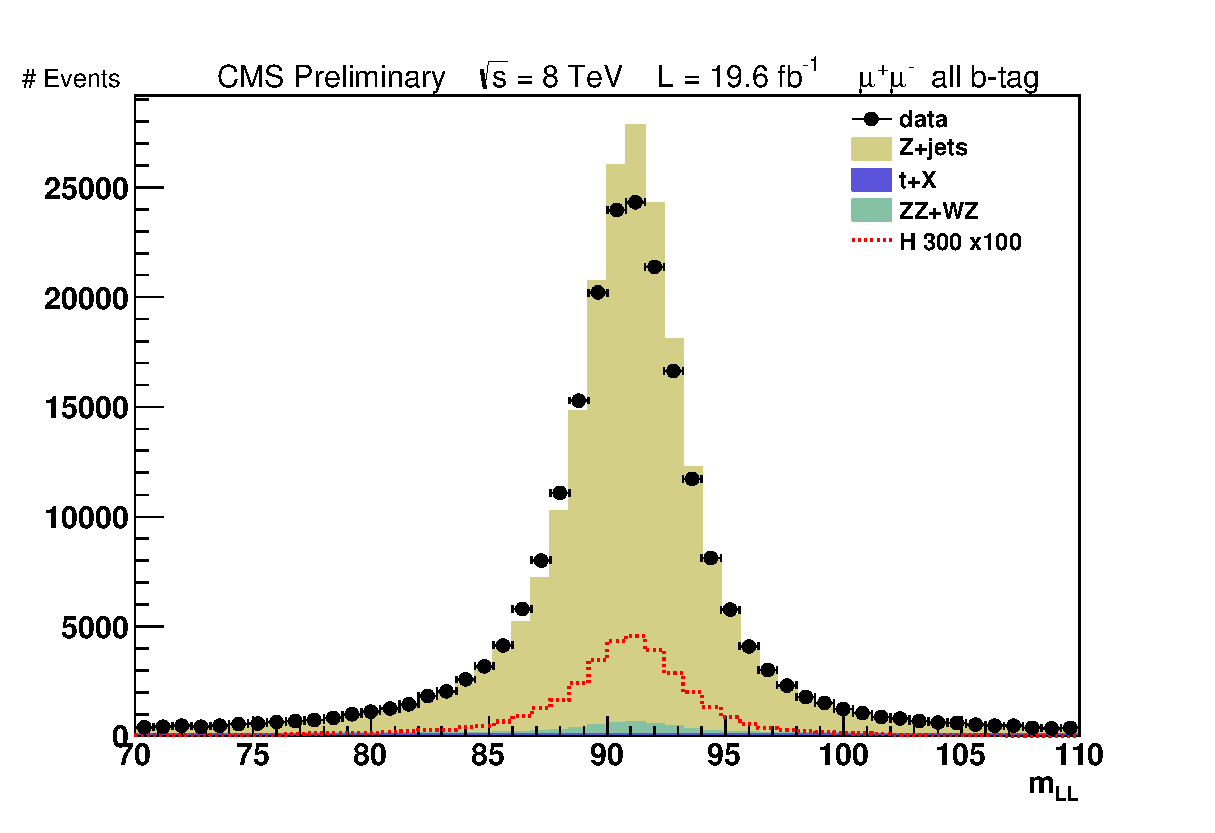
\includegraphics[width=0.45\textwidth]{presentation/defense/images/preselection/mu/mLL.eps}
\includegraphics[width=0.45\textwidth]{presentation/defense/images/preselection/el/mLL.eps}
%\includegraphics[width=0.45\textwidth]{plots//tmva_massZll.eps}
}
\caption{
Di-lepton invariant mass in data and MC of $Z \rightarrow \ell \ell$ candidates after lepton selection. Left: Muon channel. Right: Electron channel. The selection described in preselection is applied except for the cut on $m_{jj}$.
}
\label{fig:m_dilepton}
\end{center}
\end{figure}
%%%%%%%%%%%%%%%%%%%%%%%

\subsection{Jet Selection}
\label{sec:jetsel}
The PF jets are reconstructed with the anti-k$_{T}$ algorithm ~\cite{antikt} with radius parameter set to $R=0.5$. Jets are required to be inside the tracker acceptance ($|\eta|<2.4$) thus allowing high reconstruction efficiency and precise energy measurements using PF techniques. Jet-energy corrections are applied to data and Monte Carlo~\cite{CMS-PAS-JME-10-010}. Correction for PU energy is applied at the first level, by using the Fastjet algorithm~\cite{FastJet}. In order to remove jets which originate from PU interactions, only jets with $\beta \ge 0.2$ are selected, where $\beta$ is defined as the sum of transverse momenta of all charged particles in the jet coming from the primary vertex, normalized to the total sum of transverse momenta of all charged particles in the jet. The $\beta$ distribution and efficiency can be seen in Figure~\ref{fig:beta}~\cite{2l2q115}. $Z \rightarrow q\overline{q} $ candidates are reconstructed from jet-jet pairs. In order to reject fake candidates made by low-$p_T$ jets from QCD background, both jets of the pair must have $p_T > 30 GeV$.


\begin{figure}[htb]
\begin{center}
\centerline{
\includegraphics[width=0.50\textwidth]{Selection/beta_Zmm.png}
\includegraphics[width=0.50\textwidth]{Selection/beta_eff.png}
%\includegraphics[width=0.45\textwidth]{plots//tmva_massZjj.eps}
}
\caption{
$\beta$ fraction of the total transverse momentum of charged particles in a jet that is computed from particles pointing to the primary interaction for different background and signal samples (left) and efficiency of a cut in $\beta <$ 0.2 for signal with Higgs mass of 200 GeV and 300 GeV and Z+Jets background, as a function of the number of reconstructed vertices in an event(right).~\cite{2l2q115}
}
\label{fig:beta}
\end{center}
\end{figure}


A loose jets identification is applied to the jets to remove fake jets that arise from calorimeter noise.  These requirements are summarized in table~\ref{tab:jetcuts}.  In the analysis a cut around the Z mass is done for 75 $< m_{jj} <$ 105 GeV to help control the Z+jets background.  The $m_{jj}$ distributions for electron and muon channels can be seen in Figure~\ref{fig:mjj}.
%%%%%%%%%%%%%%%%%%%%%%%%%%%%%%%%
\begin{table*}[htb!]
\caption{ 
Jet cuts to remove fakes.
}
\label{tab:jetcuts}
\vspace*{\medskipamount}
\begin{center}
\small
\begin{tabular}{|l|l|}
\hline
Variable & Cuts\\
\hline
fraction of energy due to neutral hadron & $<$ 0.99 \\
fraction of energy due to neutral EM deposits & $<$ 0.99 \\
number of constituents & $>$ 1 \\
number of charged hadrons candidates & $>$ 0 \\
fraction of energy due to charged hadron candidates & $>$ 0 \\
fraction of energy due to charged EM deposits & $<$ 0.99 \\
$\beta$ & $>=$ 0.2  \\
\hline
\end{tabular}
\end{center}
\end{table*}
%%%%%%%%%%%%%%%%%%%%%%%%%%%%%%%%%%%%%%%%%%%%%%%%%

%%%%%%%%%%%%%%%%%%%%%%%
\begin{figure}[htb]
\begin{center}
\centerline{
\includegraphics[width=0.45\textwidth]{presentation/defense/images/preselection/mu/mJJ.eps}
\includegraphics[width=0.45\textwidth]{presentation/defense/images/preselection/el/mJJ.eps}
%\includegraphics[width=0.45\textwidth]{plots//tmva_massZjj.eps}
}
\caption{
Di-jet invariant mass in data and MC for $\ell \ell jj$ candidates which have passed the preselection. Left: Muon channel. Right: Electron channel.
}
\label{fig:mjj}
\end{center}
\end{figure}
%%%%%%%%%%%%%%%%%%%%%%%

\subsection{B-tagging of jets}
\label{subsec:btaggingofjets}
Due to the relatively large branching fraction of the $Z$-bosons decaying into a pair of bottom-anti-bottom quarks, compared to the abundance of light-quark or gluon jets in $Z$+jets background events, we use a b-tagging algorithm in order to identify jets originating from heavy-flavor quarks. However, no selection of candidates based on b-probabilities is employed in the analysis. Instead, the b-tagging information is used to classify $\ell \ell jj$ candidates into three categories, each one characterized by a certain signal-to-background ratios, and an optimized selection is applied on candidates belonging to different categories~\cite{CMS-AN-2011-399}. This exploits as much information as possible from the data increasing the analysis sensitivity.

With Z+jets as the main background, this is primarily described by a Z boson that decays leptonically in conjunction with the production of high $p_T$ jets. These jets are primarily produced from gluon radiation as well as light quark hadronization.  These light quarks come from the fact that u and d quarks make up the valence partons of the proton. One of the main differences for signal and background is that the signal will not contain gluons, and relative to the background, will have a large contribution of heavy flavor quarks.

We are using the CMS Jet Probability (JP) tagging algorithm for b-jets~\cite{CMS-PAS-BTV-11-004}.  This uses the relative long lifetime of bottom hadrons with the tracks from the PF algorithms to estimate if the jet came from the primary vertex.  If this probably is low then the jet has a larger probability of being a b-jet.  The good performance of this b-jet identification is possible because of the the precision tracking of charged particles and lepton identification at CMS.

The output of the JP algorithm is a discriminator for each jet in the event.  This distribution for data and simulated events can be seen in Figure~\ref{fig:JP} for electrons and muons.  To discriminate between jets that are coming from heavy flavor quarks (c,b) with those coming from light flavor quarks (d,u,s) we use two separate values from the JP algorithm.  The first point, called the loose working point (L), is set at a value of the output of the JP algorithm equal to 0.0275. This working point corresponds to a mis-identification probability that the jet is a light flavored jet of 10\%.  The medium working point (M) has a value of 0.545 and has a mis-identification probability of 1\%.  These are abbreviated as JPL and JPM for the loose and medium working points respectively.


A summary of all the selection can be found in section~\ref{sec:summaryofselectionrequirements}.
%Details of the b-tagging algorithm are described in section%~\ref{sec:btag} and candidates 
%categories are defined in section%~\ref{ssec:classification}


%%%%%%%%%%%%%%%%%%%%%%%
\begin{figure}[htb]
\begin{center}
\centerline{
\includegraphics[width=0.49\textwidth]{presentation/defense/images/preselection/mu/j0jp_log.eps}
\includegraphics[width=0.49\textwidth]{presentation/defense/images/preselection/el/j0jp_log.eps}
%\includegraphics[width=0.45\textwidth]{plots//tmva_massZjj.eps}
}
\caption{
Distribution of the jet probability (JP) discriminator that is used for b-tagging.  Right: Muons. Left: Electrons. The peaks in the distribution come from calculating the jet probability non-continuously in $\eta$ bins. This phenomenon is well understood and expected.
}
\label{fig:JP}
\end{center}
\end{figure}
%%%%%%%%%%%%%%%%%%%%%%%


\subsection{Higgs candidates}
\label{sec:reco}
All the leptons and jets that satisfy the above requirements are combined to form both leptonic and hadronic Z bosons.  For each event, the dilepton and dijet pairs are combined to create $\ell \ell jj$ events or Higgs candidates. A $\Delta R > 0.5$ cut is applied between each lepton and jet within a candidate in order to avoid double counting of the same object reconstructed in different collections (for instance leptons inside a jet). An example event with a Higgs boson candidate decaying to two muons and two jets can be seen in Figure~\ref{fig:event_display}~\cite{CMS-PAS-HIG-12-024}. In the following sections, the previous requirements on Higgs candidates and their constituent particles will be referred to as preselection.

%%%%%%%%%%%%%%%%%%%%%%%
\begin{figure}[htb]
\begin{center}
\centerline{
\includegraphics[width=0.85\textwidth]{Selection/eventDisplay7TeV.png}
%\includegraphics[width=0.45\textwidth]{plots//tmva_massZjj.eps}
}
\caption{
An event display of a Higgs event candidate decaying to two muons and two jets.~\cite{CMS-PAS-HIG-12-024}
}
\label{fig:event_display}
\end{center}
\end{figure}
%%%%%%%%%%%%%%%%%%%%%%%




\chapter{Signal Optimization}


After the preselection, additional selection criteria is performed to optimize the discrimination power for a Higgs signal.

\section{Tagging Classification}

Once the events are preselected as described in the previous sections, they are classified according to the b-tagging (see section~\ref{subsec:btaggingofjets})  of the jets associated to the Higgs candidate. Events are classified as ``two tags'' if the two jets are b-tagged with at least one medium-tag and one loose-tag. Events failing that requirement are classified as ``one tag'' if at least one of the two jets satisfy the loose-tag condition. Events failing this requirement are finally classified as ``no-tag''.  These three categories are mutually exclusive.  A summary can be seen in Table~\ref{tab:btagcateg}.

%%%%%%%%%%%%%%%%%%%%%%%%%%%%%%%%
\begin{table*}[htb!]
\caption{ 
B-tag categories.
}
\label{tab:btagcateg}
\vspace*{\medskipamount}
\begin{center}
\small
\begin{tabular}{|c|c|}
\hline
Tag Region & Description\\
\hline
0-tag & jet is not tagged Loose; other jet is not tagged Loose \\
1-tag & jet is tagged Loose; other jet is not tagged Medium \\
2-tag & jet is tagged Medium; other jet is tagged Loose \\
\hline
\end{tabular}
\end{center}
\end{table*}
%%%%%%%%%%%%%%%%%%%%%%%%%%%%%%%%%%%%%%%%%%%%%%%%%

As these three categories present very different signal-to-background ratios they are treated separately in the final optimization. In addition, some differences in the selection are also needed due to the different background composition, especially in the case of the ``two tags'' sample, in which the $t\overline{t}$ background starts to be noticeable. On the other hand, since the optimization is based mostly on the intrinsic properties of the final state under investigation, there are analysis strategies that are shared by the three categories. The main differences between the categories are that the 2 b-tag category has the highest purity, but has very low signal yield.  Opposed to that, the 0 b-tag category has the largest signal yield but is dominated by Z+jets background. The 1 b-tag category is affected by both issues and therefore has the least discriminating power.

There are differences in the b-tagging between data and those predicted by Monte Carlo.  These differences are corrected by b-tagging scale factors.  These are used to adjust two different problems.  The first is the efficiency that the JP algorithm will not recognize a b-jet even if it is from a heavy flavored quark.  Second, the light quarks or gluons are incorrectly identified as b-jets.  

The efficiency ($SF_{hf}$) (from non tagging of heavy quarks) and the mis-identification rate ($SF_{lf}$) (labeling light quarks and gluons as b-jets) are defined as the ratio of tagging efficiency between heavy and light flavor jets in data and simulations.  These are typically functions of $p_T$ and the pseudo-rapidity of the jets.  Typically $SF_{hf}$ is smaller than one because in data the successful tagging of heavy quarks is better than in simulation.  Oppositely, $SF_{lf}$ is typically larger than one because tagging light quarks in data as b-jets is more common than in simulation.  In general all jets, regardless of flavor, are tagged as b-jets more frequently in data than jets in simulation~\cite{CMS-PAS-BTV-11-004}.

The b-tagging performance is corrected between data and simulation, but we must take additional steps than simply scaling the JP distribution.  This is because our classification of events is based on the jet flavor of both tagged and non-tagged jets.  The process to correctly distribute candidates between the categories is as follows.  As the scale factors change the jets momentum there is a percentage of jets that would migrate to a different b-tagged category. Using a random number generator candidates are upgraded or downgraded between the different b-tagging categories according to the scale factor percentages. This gives jets that are tagged a non zero chance of being lowered to another category or non-tagged jets to be raised to a higher category.  For example, a medium-tagged jet can be lowered to a loose-tagged jet, or a loose-tagged jet can be lowered to a non-tagged jet.  Also, a non-tagged jet can be promoted to a loose-tagged jet, or a loose-tagged jet can be promoted to a medium-tagged jet~\cite{2l2q115}.


\section{Helicity Likelihood}

There are a number of kinematic differences between the $H \rightarrow ZZ \rightarrow 2l2q$ decay and the Z + jets background.  When a heavy Higgs boson is produced and decays into two Z bosons, those Z bosons have boosted kinematics.  The $p_T$ of the Z bosons increases with the mass of the parent particle, the Higgs boson.  Another powerful variable to separate signal from background is the $\Delta R$ spacing between the two jets, leptons, and Z bosons.  This space decreases as the boost of the Z bosons increases and is similarly correlated to the reconstructed Higgs mass as can be seen in Figure~\ref{fig:nousevars}.  Since we use the invariant mass of the reconstructed Higgs candidate as the main discriminating variable, these kinematic variables are problematic to use. Also, the variable selection criteria would need to be parameterized as a function of the reconstructed di-boson invariant mass.

%%%%%%%%%
\begin{figure}[htb!]
%\begin{center}
\centerline{
\includegraphics[width=0.45\textwidth]{Optimization/mzz_ptLL_background.eps}
\includegraphics[width=0.45\textwidth]{Optimization/mzz_ptLL_300.eps}
}
\centerline{
\includegraphics[width=0.45\textwidth]{Optimization/mzz_ptJJ_background.eps}
\includegraphics[width=0.45\textwidth]{Optimization/mzz_ptJJ_300.eps} \\
}
\centerline{
\includegraphics[width=0.45\textwidth]{Optimization/mzz_jjdr_background.eps}
\includegraphics[width=0.45\textwidth]{Optimization/mzz_jjdr_300.eps} \\
%\includegraphics[height=2.5in]{plots/angles-Graviton-all2}
}
%\end{center}
\caption{Various kinematic variables comparing Z+Jets background and Higgs of 300 GeV simulations to demonstrate the correlation between the kinematics and $m_{ZZ}$.  (Top Left) $p_T (ll)$ vs $m_{ZZ}$ for Z+Jets.  (Top Right) $p_T (ll)$ vs $m_{ZZ}$ for Higgs 300. (Middle Left) $p_T (jj)$ vs $m_{ZZ}$ for Z+Jets.  (Middle Right) $p_T (jj)$ vs $m_{ZZ}$ for Higgs 300. (Bottom Left) $\Delta R_{jj}$ vs $m_{ZZ}$ for Z+Jets.  (Bottom Right) $\Delta R_{jj}$ vs $m_{ZZ}$ for Higgs 300. 
\label{fig:nousevars}}  
\end{figure}
%%%%%%%%%

The signal topology is affected by the production of a heavy Higgs.  These topological features are not limited to only the kinematics of the final state particles but have other manifestations as well.  This is because the decay of a spin-0 boson decays to a pair of identical spin-1 bosons which decay to fermions.  For us, the spin-0 boson is the Higgs and the spin-1 bosons are the Z bosons.  This well defined spin correlation will be seen in the angular distribution of the final state particles.  The probability density functions of the angles can be computed analytically for Higgs signals~\cite{Physics_2010}.  The background is not resonant so there is no spin correlation and thus there are different angular distributions for the final states between Z+Jets and the signal.  This topology difference is not unique to the Higgs boson and can also help in the search for other particles~\cite{PhysRevD.81.075022}. 

The decay kinematics in the signal $H \rightarrow ZZ \rightarrow 2l2q$ have several distinct features that can be used to discriminate against background. Five angular observables fully describe the angular distribution of the decay products in $2 \rightarrow 1 \rightarrow 2 \rightarrow 4$ as in $ab \rightarrow X \rightarrow ZZ \rightarrow 2l2j$ ~\cite{Gao_5angles,Rujela_5angles}. There are three helicity angles $\theta_1, \theta_2,$ and $\Phi$, as well as two production angels $\theta^*$ and $\Phi_1$.  Additionally, they are orthogonal to the three invariant masses of the $X$ and the two $Z$ and to the longitudinal and transverse momenta of the $X$. The orthogonal observables are largely uncorrelated and are useful for event selection beyond using them as raw kinematic observables. The definitions of these variables can be found in Table~\ref{tab:5anglesdef}.
Fig.~\ref{fig:decay} illustrates the angular distribution in the production and decay chain $ab\to X\to P_1P_2\to p_{11}p_{12}p_{21}p_{22}$ with an example of the $ab\to X\to ZZ\to 2\ell2q$ chain with two partons $a$ and $b$, such as $gg$ or $q\bar{q}$.

%%%%%%%%%%%%%%%%%%%%%%%%%%%%%%%%
\begin{table*}[htb!]
\caption{ 
Definitions of the 5 angular variables describing events of the form $ab \rightarrow X \rightarrow ZZ \rightarrow 2l2j$ as seen in Figure~\ref{fig:decay}.
}
\label{tab:5anglesdef}
\vspace*{\medskipamount}
\begin{center}
\small
\begin{tabularx}{\textwidth}{|c|X|}
%\begin{tabular}{|c|l|}
\hline
Variable & Definition\\
\hline
$\theta_1$ & The angle between the direction of the $\Plm$ (from $Z \rightarrow \Plp \Plm$) and the direction opposite the X in the Z rest frame. \\ \hline
$\theta_2$ & The angle between the direction of the $\Pq$ (from $Z \rightarrow \Pq \Paq$) and the direction opposite the X in the Z rest frame. \\ \hline
$\Phi$ & The angle between the decay planes of the two Z decays. \\ \hline
$\theta^*$ & The angle between the parton collision axis ($z$) and the decay axis in the rest frame ($z^`$). \\ \hline
$\Phi_1$ & The angle between the production plane and the $Z \rightarrow \Plp \Plm$ decay plane. \\
\hline
\end{tabularx}
\end{center}
\end{table*}
%%%%%%%%%%%%%%%%%%%%%%%%%%%%%%%%%%%%%%%%%%%%%%%%%


%%%%%%%%%
\begin{figure}[htb!]
%\begin{center}
\centerline{
\includegraphics[height=2.5in]{plots/angles-HZZ2l2q}
%\includegraphics[height=2.5in]{plots/angles-Graviton-all2}
}
%\end{center}
\caption{Diagram depicting the decay $X\rightarrow ZZ\rightarrow 2l2q$ and the 5 decay angles which describe it.
\label{fig:decay}}
\end{figure}
%%%%%%%%%


The angular distributions for data and simulations can be found in Figures~\ref{helicityDistDataMCE0},~\ref{helicityDistDataMCE1}, and~\ref{helicityDistDataMCE2} for electrons and in Figures~\ref{helicityDistDataMCM0},~\ref{helicityDistDataMCM1}, and~\ref{helicityDistDataMCM2} for muons.  These figures show the differences between the samples in each of the b-tag regions.  Because the background does not have spin correlation, there is a difference between the simulated signal, the background simulation, and data.  Also, you can see similar performance between electrons and muons, as well as between different b-tag categories.  This similarity between muons and electrons, as well as between b-tag categories, is expected and will be used to simplify the analysis by doing common final selection between lepton types and b-tag categories.


%%%%%%%%%%%%%
\begin{figure}[thb!]
\centerline{
\includegraphics[width=0.33\textwidth]{presentation/defense/images/preselection/0/el/costheta1.eps}
\includegraphics[width=0.33\textwidth]{presentation/defense/images/preselection/0/el/costheta2.eps}
\includegraphics[width=0.33\textwidth]{presentation/defense/images/preselection/0/el/costhetast.eps}
}
\centerline{
\includegraphics[width=0.33\textwidth]{presentation/defense/images/preselection/0/el/phi.eps}
\includegraphics[width=0.33\textwidth]{presentation/defense/images/preselection/0/el/phi1.eps}
}
\caption{
Five angular distributions of $\cos\theta_1, \cos\theta_2, \cos\theta^*, \Phi$, $\Phi_1$ and the helicity likelihood discriminant for 2012 electron data (points) and Summer 2012 Monte Carlo samples (histogram) in the 0 b-tag category.  The red line is the expected distribution for a Higgs boson with mass 300 GeV.  The selection is as described in preselection.
\label{helicityDistDataMCE0}}
\end{figure}
%%%%%%%%%%%%%
%%%%%%%%%%%%%
\begin{figure}[thb!]
\centerline{
\includegraphics[width=0.33\textwidth]{presentation/defense/images/preselection/1/el/costheta1.eps}
\includegraphics[width=0.33\textwidth]{presentation/defense/images/preselection/1/el/costheta2.eps}
\includegraphics[width=0.33\textwidth]{presentation/defense/images/preselection/1/el/costhetast.eps}
}
\centerline{
\includegraphics[width=0.33\textwidth]{presentation/defense/images/preselection/1/el/phi.eps}
\includegraphics[width=0.33\textwidth]{presentation/defense/images/preselection/1/el/phi1.eps}
}
\caption{
Five angular distributions of $\cos\theta_1, \cos\theta_2, \cos\theta^*, \Phi$, $\Phi_1$ and the helicity likelihood discriminant for 2012 electron data (points) and Summer 12 Monte Carlo samples (histogram) in the 1 b-tag category.  Open histograms indicate the expected distribution for a Higgs boson with mass 300 GeV. The selection is as described in preselection.
\label{helicityDistDataMCE1}}
\end{figure}
%%%%%%%%%%%%%
%%%%%%%%%%%%%
\begin{figure}[thb!]
\centerline{
\includegraphics[width=0.33\textwidth]{presentation/defense/images/preselection/2/el/costheta1.eps}
\includegraphics[width=0.33\textwidth]{presentation/defense/images/preselection/2/el/costheta2.eps}
\includegraphics[width=0.33\textwidth]{presentation/defense/images/preselection/2/el/costhetast.eps}
}
\centerline{
\includegraphics[width=0.33\textwidth]{presentation/defense/images/preselection/2/el/phi.eps}
\includegraphics[width=0.33\textwidth]{presentation/defense/images/preselection/2/el/phi1.eps}
}
\caption{
Five angular distributions of $\cos\theta_1, \cos\theta_2, \cos\theta^*, \Phi$, $\Phi_1$ and the helicity likelihood discriminant for 2012 electron data (points) and Summer 12 Monte Carlo samples (histogram) in the 2 b-tag category.  Open histograms indicate the expected distribution for a Higgs boson with mass 300 GeV. The selection is as described in preselection.
\label{helicityDistDataMCE2}}
\end{figure}
%%%%%%%%%%%%%
%**********Muons******************%
%%%%%%%%%%%%%
\begin{figure}[thb!]
\centerline{
\includegraphics[width=0.33\textwidth]{presentation/defense/images/preselection/0/mu/costheta1.eps}
\includegraphics[width=0.33\textwidth]{presentation/defense/images/preselection/0/mu/costheta2.eps}
\includegraphics[width=0.33\textwidth]{presentation/defense/images/preselection/0/mu/costhetast.eps}
}
\centerline{
\includegraphics[width=0.33\textwidth]{presentation/defense/images/preselection/0/mu/phi.eps}
\includegraphics[width=0.33\textwidth]{presentation/defense/images/preselection/0/mu/phi1.eps}
}
\caption{
Five angular distributions of $\cos\theta_1, \cos\theta_2, \cos\theta^*, \Phi$, $\Phi_1$ and the helicity likelihood discriminant for 2012 muon data (points) and Summer 12 Monte Carlo samples (histogram) in the 0 b-tag category.  The red line is the expected distribution for a Higgs boson with mass 300 GeV.  The selection is as described in preselection.
\label{helicityDistDataMCM0}}
\end{figure}
%%%%%%%%%%%%%
%%%%%%%%%%%%%
\begin{figure}[thb!]
\centerline{
\includegraphics[width=0.33\textwidth]{presentation/defense/images/preselection/1/mu/costheta1.eps}
\includegraphics[width=0.33\textwidth]{presentation/defense/images/preselection/1/mu/costheta2.eps}
\includegraphics[width=0.33\textwidth]{presentation/defense/images/preselection/1/mu/costhetast.eps}
}
\centerline{
\includegraphics[width=0.33\textwidth]{presentation/defense/images/preselection/1/mu/phi.eps}
\includegraphics[width=0.33\textwidth]{presentation/defense/images/preselection/1/mu/phi1.eps}
}
\caption{
Five angular distributions of $\cos\theta_1, \cos\theta_2, \cos\theta^*, \Phi$, $\Phi_1$ and the helicity likelihood discriminant for 2012 muon data (points) and Summer 12 Monte Carlo samples (histogram) in the 1 b-tag category.  Open histograms indicate the expected distribution for a Higgs boson with mass 300 GeV. The selection is as described in preselection.
\label{helicityDistDataMCM1}}
\end{figure}
%%%%%%%%%%%%%
%%%%%%%%%%%%%
\begin{figure}[thb!]
\centerline{
\includegraphics[width=0.33\textwidth]{presentation/defense/images/preselection/2/mu/costheta1.eps}
\includegraphics[width=0.33\textwidth]{presentation/defense/images/preselection/2/mu/costheta2.eps}
\includegraphics[width=0.33\textwidth]{presentation/defense/images/preselection/2/mu/costhetast.eps}
}
\centerline{
\includegraphics[width=0.33\textwidth]{presentation/defense/images/preselection/2/mu/phi.eps}
\includegraphics[width=0.33\textwidth]{presentation/defense/images/preselection/2/mu/phi1.eps}
}
\caption{
Five angular distributions of $\cos\theta_1, \cos\theta_2, \cos\theta^*, \Phi$, $\Phi_1$ and the helicity likelihood discriminant for 2012 muon data (points) and Summer 12 Monte Carlo samples (histogram) in the 2 b-tag category.  Open histograms indicate the expected distribution for a Higgs boson with mass 300 GeV. The selection is as described in preselection.
\label{helicityDistDataMCM2}}
\end{figure}
%%%%%%%%%%%%%

\subsection{Angular Discriminant}

The information from the angular variables in the final state particles can be used to define a likelihood discriminate.  This likelihood discriminate allows us to select the topology that is consistent with a Higgs decay.  The first step in creating the likelihood discriminate is to build the probability density functions  for both the signal and background events.  After these have been defined we use them to get a probability ratio as seen in Equation~\ref{eq:LD} where LD is the likelihood discriminant, $P_{sig}$ is the probability the candidate is signal, and $P_{BG}$ is the probability the candidate is background.
  \begin{equation} LD = \dfrac{P_{sig}}{P_{sig}+P_{BG}} \label{eq:LD}\end{equation}

This definition puts candidates that have a topology like the signal to have a LD value close to 1 and those candidates with a topology similar to those of the background will have a LD value closer to 0.  This allows us to use this LD variable (in the future referenced to as helyLD or helicity LD) for event selection by requiring candidates to have a value higher than a certain threshold.

The function $P_{sig}$ (Equation~\ref{eq:psig}) is defined as the ideal probability function~\cite{PhysRevD.81.075022} ($P_{ideal}$) multiplied by four 1D acceptance functions.  
\begin{equation} P_{sig} = P_{ideal}(\theta_1, \theta_2, \theta^*, \Phi, \Phi_1 ;M)G_{\theta_1}(\theta_1;M)G_{\theta_2}(\theta_2;M)G_{\theta^*}(\theta^*;M)G_{\Phi_1}(\Phi_1;M) \label{eq:psig}\end{equation}

In Equation~\ref{eq:psig} M is the mass of the reconstructed Higgs candidate and the acceptance functions ($G_{\theta_1},G_{\theta_2},G_{\theta^*},G_{\Phi_1}$) are empirically calculated by fitting the signal Monte Carlo Simulations.

Similar to data, the probability distribution function for background is given in Equation~\ref{eq:psigback}.
\begin{equation} P_{BG} = P_{\theta_1}(\theta_1;M)P_{\theta_2}(\theta_2;M)P_{\theta^*}(\theta^*;M)P_{\Phi_1}(\Phi_1;M)P_{\Phi^*}(\Phi^*;M) \label{eq:psigback}\end{equation}

Each probability function is obtained entirely empirically from the fits to the simulation background Monte Carlo samples.

The acceptance functions are created for each angular variable through a number of steps.  First we define a number of bins around a central Higgs mass that we are looking at.  Then, using signal samples in these bins, we fit each angular variable to a polynomial.  The list of polynomials can be seen in Table~\ref{tab:poly}.  An example fitting for the acceptance functions a reconstructed Higgs mass of 500 GeV can be seen in Figure~\ref{fig:500fit}.
%%%%%%%%%%%%%%%%%%%%%%%%%%%%%%%%%
\begin{center}
\begin{table}[htb]
\caption{%
  \small The polynomials used for fitting each angular variable.%
}
\begin{center}
\begin{tabular}{ c c }
Variable  & Polynomial \\ \hline
$\cos(\theta_1)$ & $a_2 x^2+a_4 x^4$ \\
$\cos(\theta_2)$ & $a_2 x^2+a_4 x^4$ \\
$\cos(\theta^*)$ & $a_2 x^2+a_4 x^4+a_6 x^6$\\
$\Phi$ &   $1 + a_0 cos(x) + a_1 cos(2x)$\\
$\Phi_1$ & $1 + a_0 cos(x) + a_1 cos(2x);$ \\
\end{tabular}
\end{center}
\label{tab:poly}
\end{table}
\end{center}
%%%%%%%%%%%%%%%%%%%%%%%%%%%%%%%%
%%%%%%%%%%%%
\begin{figure}[htb!]
\begin{center}
\centerline{
\includegraphics[width=0.33\textwidth]{presentation/defense/images/plots/sigPDF_CosTheta1proj_500.pdf}
\includegraphics[width=0.33\textwidth]{presentation/defense/images/plots/sigPDF_CosTheta2proj_500.pdf}
\includegraphics[width=0.33\textwidth]{presentation/defense/images/plots/sigPDF_CosThetaSproj_500.pdf}
}
\centerline{
\includegraphics[width=0.33\textwidth]{presentation/defense/images/plots/sigPDF_Phiproj_500.pdf}
\includegraphics[width=0.33\textwidth]{presentation/defense/images/plots/sigPDF_PhiStar1proj_500.pdf}
}
\centerline{
\includegraphics[width=0.33\linewidth]{Optimization/poly_fit/costheta1/500.eps}
\includegraphics[width=0.33\linewidth]{Optimization/poly_fit/costheta2/500.eps}
\includegraphics[width=0.33\linewidth]{Optimization/poly_fit/costhetastar/500.eps}
}
\centerline{
\includegraphics[width=0.33\linewidth]{Optimization/poly_fit/phi/500.eps}
\includegraphics[width=0.33\linewidth]{Optimization/poly_fit/phi1/500.eps}
}
\caption{
Fitting the angular variables for a reconstructed Higgs mass of 500 GeV in signal Monte Carlo samples(first 5 plots) and for the Z+Jets background samples (bottom 5 plots). These are taken in a mass window of 450 GeV to 550 GeV in the ZZ invariant mass distribution.
}
\label{fig:500fit}
\end{center}
\end{figure}
%%%%%%%%%%%%

After the polynomials are fit for the range of reconstructed Higgs masses coefficients of the polynomials are then fit with a polynomial to parameterize the fits as a function of the ZZ invariant mass. This allows the acceptance functions to be a function of only the ZZ invariant mass and extends the function to be continuous for the Higgs mass values that we do not have Monte Carlo simulations for.  An example of calculating the parameters can be seen in Figure~\ref{fig:fit_poly} for $\cos(\theta_1)$.  Similar fitting is done for the other angular variables.  Figure~\ref{fig:fit_param} shows the differences for the acceptance function $G_{\theta^*}(\theta^*;450)$ between a direct fit and using the extrapolation used to get the parameritization of the polynomial coefficients.


%%%%%%%%%%%%
\begin{figure}[htb!]
\begin{center}
\centerline{
\includegraphics[width=0.33\textwidth]{Optimization/a2.pdf}
\includegraphics[width=0.33\textwidth]{Optimization/a4.pdf}
\includegraphics[width=0.33\textwidth]{Optimization/a6.pdf}
}
\caption{
Fitting the parameters $a_2$ (left), $a_4$ (middle), $a_6$ (right) for $\cos(\theta_1)$ to calculate the acceptance function $G_{\theta_1}(\theta_1;M)$ as a function of the reconstructed Higgs mass.  The same fitting is done for the other angular variables.
}
\label{fig:fit_poly}
\end{center}
\end{figure}
%%%%%%%%%%%%

%%%%%%%%%%%%
\begin{figure}[htb!]
\begin{center}
\centerline{
\includegraphics[width=0.49\textwidth]{Optimization/costhetast_450_fit.pdf}
\includegraphics[width=0.49\textwidth]{Optimization/costhetast_450_extrap.pdf}
}
\caption{A $\cos(\theta^*)$ comparison for the 450 GeV reconstructed Higgs mass signal simulations fitting the  acceptance function $G_{\theta_1}(\theta_1;M)$ directly to data (right), and plotting $G_{\theta_1}(\theta_1;450)$ from the extrapolated polynomial coefficients (left). There is very good agreement between the fitting and extrapolation.  
}
\label{fig:fit_param}
\end{center}
\end{figure}
%%%%%%%%%%%%

With these functions defined, we can then calculate the helicity likelihood discriminant as a function of the ZZ invariant mass.  Figure~\ref{fig:hely_LD} shows the distributions for the HelyLD in the 2012 data for both electrons and muons as well as an example of the shape of signal for a Higgs mass of 300 GeV.  This is shown for each of the 3 b-tag regions.  We can see that particularly in the 0-tag and 1-tag regions this is a powerful discriminating variable for the Z+Jets background.  In the 2-tag region the $\Pqt \Paqt$ background is much more prevalent, but this selection is still powerful against the Z+Jets.  


%%%%%%%%%%%%
\begin{figure}[htb!]
\begin{center}
\centerline{
\includegraphics[width=0.45\textwidth]{presentation/defense/images/preselection/0/el/helyLD.eps}
\includegraphics[width=0.45\textwidth]{presentation/defense/images/preselection/0/mu/helyLD.eps}
}
\centerline{
\includegraphics[width=0.45\textwidth]{presentation/defense/images/preselection/1/el/helyLD.eps}
\includegraphics[width=0.45\textwidth]{presentation/defense/images/preselection/1/mu/helyLD.eps}
}
\centerline{
\includegraphics[width=0.45\textwidth]{presentation/defense/images/preselection/2/el/helyLD.eps}
\includegraphics[width=0.45\textwidth]{presentation/defense/images/preselection/2/mu/helyLD.eps}
}
\caption{
HelyLD for electrons (right) and muons(left) for the 3 b-tag categories, 0-tag (top), 1-tag (middle), 2-tag (bottom). The preselection is applied to this data and the 300 GeV signal Monte Carlo is scaled by 100 to get a better picture of the comparison.
}
\label{fig:hely_LD}
\end{center}
\end{figure}
%%%%%%%%%%%%


There is a discrepancy between the data and Monte Carlo simulated samples, in that the data is more background like than simulation suggests. This is caused by the simulated Z+Jets samples not correctly representing data in the $\cos(\theta^*)$ samples.  This discrepancy can be seen in Figure~\ref{fig:costhetast} and is in the range of 0.8 $< |\cos(\theta^*)| <$ 1.0.  If we keep only events in which $|\cos(\theta^*)| <$ 0.8 then the HelyLD distribution between data and simulation is within good agreement, as can be seen in Figure~\ref{fig:helyld_cut_costhetast}.  Similar studies have been done scaling the simulation to data resulting in a correction of the HelyLD distribution.  While these measures will correct the distribution, this region of disagreement is rejected from the analysis later and there is no significant difference on the final yields between correcting the $\cos(\theta^*)$ distribution or not. Because of these reasons we do not apply any corrections to the HelyLD distribution.


%%%%%%%%%%%%
\begin{figure}[htb!]
\begin{center}
\centerline{
\includegraphics[width=0.45\textwidth]{presentation/defense/images/preselection/el/costhetast.eps}
\includegraphics[width=0.45\textwidth]{presentation/defense/images/preselection/mu/costhetast.eps}
}
\caption{$\cos(\theta^*)$ distributions for electrons (right) and muons (left). The mismatch between simulation an data can be seen in the range 0.8 $< |\cos(\theta^*)| <$ 1.0. 
}
\label{fig:costhetast}
\end{center}
\end{figure}
%%%%%%%%%%%%
%%%%%%%%%%%%
\begin{figure}[htb!]
\begin{center}
\centerline{
\includegraphics[width=0.45\textwidth]{presentation/defense/images/costhetast_cut/el/helyLD.eps}
\includegraphics[width=0.45\textwidth]{presentation/defense/images/costhetast_cut/mu/helyLD.eps}
}
\caption{HelyLD distribution after applying the selection 0.8 $< |\cos(\theta^*)|$ showing much better agreement between Monte Carlo simulation and data.
}
\label{fig:helyld_cut_costhetast}
\end{center}
\end{figure}
%%%%%%%%%%%%




%\section{Neural Network}
%\label{sec:NN}

%=================================================================
\section{Signal Optimization Based on Helicity Neural Network}
The Helicity LD is such an important part of the analysis that a cross check on its performance is performed.  For this a Neural Network is applied to separate Higgs signal from background using the five helicity angles of the final objects in the analysis as inputs. A training and test evaluation has been performed with the framework of the TMVA package~\cite{tmva} using the true event weight mix of Monte Carlo processes as background and Higgs Monte Carlo. Both the training and testing samples for both background and signal are constructed and events randomly mixed outside of the Neural Network.  There are 37,874 signal events and 38,378 background events evenly split between testing and training.  The Neural Network was trained on the Monte Carlo simulation generated for a hypothetical Higgs mass of 400 GeV. This training was on events that passed the previously explained preselection and the $Z$ boson mass window selection, but before the selection on MET significance which will be examined in more detail later in this section.


\subsection{Neural Network Architecture}
The architecture of the Neural Network consists of two hidden layers with N and N neurons respectively, where N is the number of variables, and one output node as shown in Figure ~\ref{fig:NNarch}.



%%%%%%%%%%%%
\begin{figure}[htb!]
\begin{center}
\centerline{
\includegraphics[width=0.6\linewidth]{Optimization/plots/NN/nn_network_architecture.pdf}
}
\caption{
Neural Network architecture used for the training.
}
\label{fig:NNarch}
\end{center}
\end{figure}
%%%%%%%%%%%%


\subsection{Helicity Neural Network}
The training and testing of the Neural Network can bee seen in Figure~\ref{fig:NNOutput}.  While there is separation between the signal and background and good agreement between testing and training, there is a definite spike in background at the same place as the signal spikes in the MLP (Multilayer perceptron neural network) training. The training was done with Monte Carlo generated for a hypothetical Higgs mass of 400 GeV, but then applied to the Monte Carlo for hypothetical Higgs masses of 300, 400, 500, and 600 GeV. This is because the angular components should not depend on Higgs mass. The distribution for all b-tag regions and multiple signal simulated samples can be seen in Figure~\ref{fig:0tag_mlp}, showing good discrimination between signal and background as well as good performance of the single 400 GeV training on the various signal samples.

%%%%%%%%%%%%
\begin{figure}[htb!]
\begin{center}
\centerline{
\includegraphics[width=0.8\linewidth]{Optimization/MLP.eps}
}
\caption{
The training is done after preselection and mixing electrons and muons.  Additionally we require at least one JP medium jet with training 400 GeV Higgs boson with a MLP neural network.
}
\label{fig:NNOutput}
\end{center}
\end{figure}
%%%%%%%%%%%%


%%%%%%%%%%%%
\begin{figure}[htb!]
\begin{center}
\centerline{
\includegraphics[width=0.8\linewidth]{Optimization/MLP_el.eps}
}
\centerline{
\includegraphics[width=0.8\linewidth]{Optimization/MLP_mu.eps}
}
\caption{
The MLP neural network distribution for electrons (top) and muons (bottom).  This training was done on the 400 GeV signal simulations, but applied to the 300, 400, 500, and 600 GeV samples to show the good agreement even training with only one sample.  The signal simulations are scaled for ease of reading.
}
\label{fig:NNOutput}
\end{center}
\end{figure}
%%%%%%%%%%%%

In addition to the MLP neural network, a Likelihood discriminant was calculated using the TMVA package to check the MLP performance using the same input parameters.  Figure~\ref{fig:windowcuts} shows the receiver operating characteristic (ROC) curve for the Helicity LD, MLP, and Likelihood discriminators. These show that when looking at the performance between the three after preselection requirements the MLP performs significantly better than the Helicity LD. However, after looking in windows of -6\%/+10\% around the generated Higgs mass we see the improvement drop away and we get very similar performance.  This shows that the MLP is training on additional information than the Helicity LD is using, but that this information is correlated to the mass of the reconstructed Higgs candidate.  


%%%%%%%%%%%%
\begin{figure}[htb!]
\begin{center}
\centerline{
\includegraphics[width=0.49\linewidth]{Optimization/pretag_ROC_full_5.eps}
\includegraphics[width=0.49\linewidth]{Optimization/pretag_ROC_win_5.eps}
}
\caption{The ROC curve for signal and background comparing the HelyLD, MLP, and an alternate training for a Likelihood Discriminant using the TMVA package after preselection (right).  The same curve is given with additional selection of -6\%/+10\% of the Higgs mass to give a better estimation of performance for the final shape analysis.
}
\label{fig:windowcuts}
\end{center}
\end{figure}
%%%%%%%%%%%%

In the 0-tag region the separation between signal and background looks similar to the training for Higgs 300, 400, and 500 GeV, but does not have much discrimination power for a Higgs of 200 GeV.  The discrimination power is virtually the same after applying an additional selection of -6\%/+10\% of the Higgs mass for all four cases. When comparing background rejection versus signal efficiency between the neural network and likelihood discriminate, the performance is for all practical purposes the same.

In the 1-tag region the separation between signal and background looks similar to the training for Higgs 300, 400, and 500 GeV, but does not have much discrimination power for a Higgs of 200 GeV.  The discrimination power is virtually the same after applying an additional selection of -6\%/+10\% of the Higgs mass for all four cases. When comparing background rejection versus signal efficiency between the neural network and likelihood discriminate the performance is for all practical purposes the same. See Figure~\ref{fig:nn_1tag_ROC}.

In the 2-tag region, after applying a selection of -6\%/+10\% of the Higgs mass, the discriminating power of the neural network is similar to the 1-tag case with poor performance for a Higgs of 200 GeV, but good separation for Higgs of 300, 400, and 500 GeV.  When comparing background rejection versus signal efficiency between the neural network and likelihood discriminate the performance is roughly the same, except for the Higgs of 200 GeV case where the neural network is consistently better than the Likelihood Discriminant. This is shown in Figure~\ref{fig:nn_2tag_ROC}.


%%%%%%%%%%%%%%%%%%%%%%%%%
\begin{figure}[htb!]
  \centerline{
    \includegraphics[width=0.5\textwidth]{presentation/defense/images/preselection/0/el/MLP.eps}
    \includegraphics[width=0.5\textwidth]{presentation/defense/images/preselection/0/mu/MLP.eps}
  }
  \centerline{
    \includegraphics[width=0.5\textwidth]{presentation/defense/images/preselection/1/el/MLP.eps}
    \includegraphics[width=0.5\textwidth]{presentation/defense/images/preselection/1/mu/MLP.eps}
  }
\centerline{
    \includegraphics[width=0.5\textwidth]{presentation/defense/images/preselection/2/el/MLP.eps}
    \includegraphics[width=0.5\textwidth]{presentation/defense/images/preselection/2/mu/MLP.eps}
  }
  \caption{
    The MLP neural network output for electrons (right column) and muons (left column) for the 0 b-tag region (top row), 1 b-tag region (center row) and 2 b-tag region (bottom row).  This is after preselection and also has a 300 GeV signal sample superimposed on the graphs multiplied by 100 for better visibility.
  }
  \label{fig:0tag_mlp}
\end{figure}
%%%%%%%%%%%%%%%%%%%%%%






%%%%%%%%%%%%
\begin{figure}[htb!]
\begin{center}
\centerline{
\includegraphics[width=0.6\linewidth]{Optimization/plots/NN/1tag_MVA_LD_ROC.pdf}
}
\caption{
Background Rejection Versus Signal Efficiency in the 1tag region comparing the Multi Variant Analysis output to the the Helicity Likelihood Discriminant for a Higgs mass of 200, 300, 400, and 500 GeV. This is calculated after preselection, $Z$ boson mass requirements, and requirements on MET significance, in a -6\%/+10\% Higgs mass window.
}
\label{fig:nn_1tag_ROC}
\end{center}
\end{figure}
%%%%%%%%%%%%

%%%%%%%%%%%%
\begin{figure}[htb!]
\begin{center}
\centerline{
\includegraphics[width=0.6\linewidth]{Optimization/plots/NN/2tag_MVA_LD_ROC.pdf}
}
\caption{
Background Rejection Versus Signal Efficiency in the 2tag region comparing the Multi Variant Analysis output to the the Helicity Likelihood Discriminant for a Higgs mass of 200, 300, 400, and 500 GeV. This is calculated after preselection, $Z$ boson mass requirements, and requirements on MET significance, in a -6\%/+10\% Higgs mass window.
}
\label{fig:nn_2tag_ROC}
\end{center}
\end{figure}
%%%%%%%%%%%%



\subsection{Extended MVA Variables}

A neural network or likelihood should be able to take advantage of more information then simply uisng the 5 decay angles as previously shown. One such variable that offers good discrimination power in the preselection region is $Z_{ll}pt$ / $\sum{pt}$, where $\sum{pt}$ is the sum of the two leptons, two jets, and the met. $Z_{ll}pt$ and $\sum{pt}$ are scalar quantities.  This variable distribution is shown in Figure~\ref{fig:zllptzumpt}. While adding this variable to a MLP training improves the discrimination power in the inclusive pretag region, once we look in a mass window of -6\%/+10\% around Higgs 400 adding $Z_{ll}pt$ / $\sum{pt}$ to the training actually lowers the discrimination power of the neural network. This same performance drop is seen when training is done with the addition of the reconstructed Higgs mass as well.

This under-performance of adding additional information to the MLP neural network is due to over training in the regions where the background will not contribute (outside of the mass window of -6\%/+10\% around Higgs).  We should be able to gain additional performance by training the samples after only looking around the Higgs mass, but the sample sizes get too small to do a multi-variate analysis.  This can be seen by looking at the high correlation between the additional variables and the reconstructed ZZ invariant mass, whereas the 5 helicity angular variables are orthogonal to the ZZ, $Z_{ll}$, and $Z_{qq}$ invariant masses.  



%While training on each Higgs mass can give additional descrimination power over trainng on one Higgs mass and applying it to multiple hypothetical Higgs masses there are some difficulties. It is more conveniant to be able to train on just one higgs mass and then apply this training to a range of hypothetical higgs masses. An example of training on a Higgs 400 GeV sample and then applying this training to various hypothetical Higgs masses is show in Figure~\ref{fig:nn_allhiggs}.  This training is for a MLP neural network tranined on the 5 decay angles. This training is applied after preselection and requiring at least one JP medium jet. This shows that good performance can be acheived using the MLP by only training on one Higgs mass sample, without the need for aditional trainings, or parameratising a descriminate as a function of the reconstructed Higgs mass.


%%%%%%%%%%%%
\begin{figure}[htb!]
\begin{center}
\centerline{
\includegraphics[width=0.5\linewidth]{Optimization/plots/NN/zllpt_sumpt.png}
\includegraphics[width=0.5\linewidth]{Optimization/plots/NN/zllpt_sumpt_window.png}
}
\caption{
Signal samples are normalized to background. Left: $\dfrac{Z_{ll}pt}{\sum{pt}}$ after preselection.  Right: $\dfrac{Z_{ll}pt}{\sum{pt}}$ after preselection and 376 $<$ $m_{ZZ}$ $<$ 440 GeV.
}
\label{fig:zllptzumpt}
\end{center}
\end{figure}
%%%%%%%%%%%%


%%%%%%%%%%%%
\begin{figure}[htb!]
\begin{center}
\centerline{
\includegraphics[width=0.5\linewidth]{Optimization/plots/NN/pretag_ROC_400.pdf}
\includegraphics[width=0.5\linewidth]{Optimization/plots/NN/pretag_ROC_400_wincut.pdf}
}
\caption{Applying a MLP training to preselection and at least one JP medium jet.  The working point is the equivalent performance of current analysis that we apply in the two tag region. The helyLD variable is shown for comparison. Left: ROC curves after preselection.  Right: ROC curves after preselection and 376 $<$ $m_{ZZ}$ $<$ 440 GeV.
}
\label{fig:zllptzumpt2}
\end{center}
\end{figure}
%%%%%%%%%%%%

%%%%%%%%%%%%
\begin{figure}[htb!]
\begin{center}
\centerline{
\includegraphics[width=0.6\linewidth]{Optimization/plots/NN/pretag_ROC_wincut.pdf}
}
\caption{
This training is for a MLP neural network trained on the 5 decay angles of a Higgs 400 GeV sample. This training is applied after preselection and requiring at least one JP medium jet to samples with a Higgs mass of 300,400, and 500 GeV. The working point is the background rejection point that we currently achieve in the two tag region in our analysis. The helyLD variable is shown for comparison.
}
\label{fig:nn_allhiggs}
\end{center}
\end{figure}
%%%%%%%%%%%%




\section{Helicity Optimization}

The Helicity likelihood discriminate is optimized using a Punzi equation as seen in Equation~\ref{eq:Punzi}~\cite{punzi}.
\begin{equation} \dfrac{sig_{eff}}{0.98 + \sqrt{B}} \label{eq:Punzi}\end{equation}

$sig_{eff}$ is the signal efficiency defined as $\dfrac{number\ of\ signal\ events}{total\ number\ of\ signal\ events}$ and B is the number of background events.  This Punzi equation is used instead of more traditional functions like $\dfrac{S}{B}$, $\dfrac{S}{\sqrt{B}}$, and $\dfrac{S}{\sqrt{S+B}}$ because we are optimizing the analysis for exclusion over discovery. This optimization is done for the MLP neural network that is trained on the helicity angles as well. A selection on 0.5 in all the regions is within 5\% of the optimal value, so instead of making our selection as a function of reconstructed ZZ invariant mass we simply apply 0.5 for all mass ranges and for all b-tag categories.  While 0.5 is a good selection for the MLP, when cross checking between the the HelyLD and the MLP we use the working points as found in Figure~\ref{fig:nn_allhiggs}. These working points correspond to efficiency we get in the main line analysis.


%%%%%%%%%%%%
\begin{figure}[htb!]
\begin{center}
\centerline{
  \includegraphics[width=0.33\textwidth]{Optimization/5ang/zero_300.eps}
 \includegraphics[width=0.33\textwidth]{Optimization/5ang/one_300.eps}
\includegraphics[width=0.33\textwidth]{Optimization/5ang/two_300.eps}
}
\centerline{
  \includegraphics[width=0.33\textwidth]{Optimization/5ang/zero_400.eps}
\includegraphics[width=0.33\textwidth]{Optimization/5ang/one_400.eps} 
\includegraphics[width=0.33\textwidth]{Optimization/5ang/two_400.eps}
}
\centerline{
  \includegraphics[width=0.33\textwidth]{Optimization/5ang/zero_500.eps}
\includegraphics[width=0.33\textwidth]{Optimization/5ang/one_500.eps}
\includegraphics[width=0.33\textwidth]{Optimization/5ang/two_500.eps}
}
\centerline{
  \includegraphics[width=0.33\textwidth]{Optimization/5ang/zero_600.eps}
 \includegraphics[width=0.33\textwidth]{Optimization/5ang/one_600.eps}
 \includegraphics[width=0.33\textwidth]{Optimization/5ang/two_600.eps}
}
\caption{
The Punzi equation $\dfrac{sig_{eff}}{0.98 + \sqrt{B}}$ for the 3 b-tag regions 0-tag (left column), 1-tag (center column), 2-tag (right column) and Higgs masses 300 (top row), 400 (second row), 500 (third row), 600 (bottom row) GeV.  Also a selection outside of the region $\pm$20\% around the Higgs masses for each sample is applied to make it similar to the final region. All plots have electrons and muons separate on each plot.
}
\label{fig:Punzi_tags}
\end{center}
\end{figure}
%%%%%%%%%%%%%%%%%%%%




\section{Missing Transverse Energy}

After doing preselection and selection using the helicity angles, the 2 b-tag category is still rich in events from $\Pqt \Paqt$ that have two b-quark jets.  Our Higgs signature $H \rightarrow ZZ \rightarrow \Plp \Plm \Pq \Paq$ in adition to the jets have two leptons.  The main background that looks like this is:  $\Pqt \Paqt \rightarrow (W^+ \rightarrow \Plp \Pgn)b (W^- \rightarrow \Plm \Pagn)\Paqb$.  This final state contains oppositely signed leptons (like signal), 2 b-jets (like signal), and two neutrinos (unlike signal).

The additional neutrinos in the final state of the $\Pqt \Paqt$ backbround give us a nice handle on this background.  Every event in the detector must conserve the total momentum in the transverse plane.  If there is an imbalance among all particles, it means that most likely there is a weakly interacting particle passing through the detector (like neutrinos). If this imbalance is seen in the event, most likely the event is not in our channel of Higgs decay due to of the lack of neutrinos in the final state.

We define MET as the quantity of transverse energy that is not detected from the events.  Reasons for this include there are gaps in the detectors, as well as finite resolution of the detector, meaning particle flow candidates may not be reconstructed at full efficiency. 

While many of these problems can be taken into account to correct the MET, another option is to look at the significance of the PF MET.  A function called MET significance can be built by using two likelihood functions; one for the likelihood that the true MET is equal to the value measured in the PF algorithm, and another likelihood which measures if the true MET is equal to zero~\cite{1748-0221-6-09-P09001}. The definition of MET significance can be found in Equation~\ref{eq:METsignificance}.
\begin{equation} MET\ Significance = 2ln\lambda(MET) = 2ln \dfrac{L(MET_{true} = MET_{measured})}{L(MET_{true} = 0)} \label{eq:METsignificance}\end{equation}

Figure~\ref{fig:metsignificance} shows the MET significance after preselection in the three b-tag categories.  While the $\Pqt \Paqt$ background is mainly a problem for the 2-tag category, we apply a selection on MET significance on all b-tag categories for constancy.  This MET significance requirement of 10 is very loose and is in the tail of the signal distribution.  This allows the systematic uncertainty for the disagreement between data and background prediction to be negligible compared to other sources of systematic uncertainty.  



%%%%%%%%%%%%%%%%%%%%%%%%%
\begin{figure}[htb!]
  \centerline{
    \includegraphics[width=0.5\textwidth]{presentation/defense/images/preselection/0/el/METsignif.eps}
    \includegraphics[width=0.5\textwidth]{presentation/defense/images/preselection/0/mu/METsignif.eps}
  }
\centerline{
    \includegraphics[width=0.5\textwidth]{presentation/defense/images/preselection/1/el/METsignif.eps}
    \includegraphics[width=0.5\textwidth]{presentation/defense/images/preselection/1/mu/METsignif.eps}
  }
\centerline{
    \includegraphics[width=0.5\textwidth]{presentation/defense/images/preselection/2/el/METsignif.eps}
    \includegraphics[width=0.5\textwidth]{presentation/defense/images/preselection/2/mu/METsignif.eps}
  }
  \caption{
    Distributions for MET significance after preselection for electrons (right column) and muons (left column) for the 0 b-tag region (top row), 1 b-tag region (center row), and 2 b-tag region (bottom row).  A signal simulation is superimposed for a Higgs 300 GeV and multiplied by 100 for ease of reading.
  }
  \label{fig:metsignificance}
\end{figure}
%%%%%%%%%%%%%%%%%%%%%%


Small differences in the MET significance of the data and the Drell-Yan Z+jets simulation are taken into account studying the region MET significance $<$ 6, where the contamination of the t+X background is reduced. It is observed that a simple multiplicative factor of 1.15 $\pm$ 0.01 brings the Monte Carlo distribution in very good agreement with the data, a factor that is stable for muons and electrons, and as a function of the number of vertices in the event~\cite{CMS-AN-HIG-13-064}. The validity of this factor has been checked up to larger values of the MET significance in a top-depleated data subsample, requiring $p_T$ of jets $<$ 20 GeV. Therefore the MET significance in the Drell-Yan, diboson and Higgs boson Monte Carlo events is multiplied by a factor 1.15. The effect of this factor on the efficiency of the MET significance is minimal (in all cases the efficiency changes by less than 1\%).



\section{Summary of Selection Requirements}
\label{sec:summaryofselectionrequirements}

The selection and preselection is the same for all b-tag categories. While there is a difference between the signal and background in each category, the additional discrimination power is negligible and for ease of analysis we use the same selection in each category.  Table~\ref{tab:full_selection_summery} shows a summary of the selection, both the preselection and the final selection.  

When there are multiple candidates per event we apply a string of logic operators to chose one candidate per event. The best candidate is selected by first looking at the signal and sideband region.  If a candidate is in the signal region it is chosen over those in the sidebands.  If there are multiple candidates per event in the signal region then the candidate is chosen according to the higher b-tag category (2 b-tags over 1 b-tag and 1 b-tag over 0 b-tags).  If there are multiple candidates in the same b-tag region then the candidate with the invariant masses of the Z bosons closest to the nominal Z boson mass is chosen. If none of the candidates make it into the signal region, the same ranking of candidates is done for all those in the sideband region. 
\begin{equation} |M_{\Plp \Plm} - m_Z| + |M_{JJ} - m_Z| \label{eq:minZ}\end{equation}

The expected yields corresponding to 19.6 $fb^{-1}$ after all the selection can be seen in Table~\ref{tab:yeilds_summery}.



%%%%%%%%%%%%%%%%%%%%%%%%%%%%%%%%
\begin{table*}[htb!]
\caption{ 
Selection on the 3 b-tag categories.
}
\label{tab:full_selection_summery}
\vspace*{\medskipamount}
\begin{center}
\small
\begin{tabular}{|l|c|c|c|}
\hline
 observable      &   0 $b$-tag   &   1 $b$-tag  &   2 $b$-tag  \\ \hline
btag & none & JPL & JPL \& JPM \\ \hline
helicity LD  &  \multicolumn{3}{|c|}{$>$ 0.5}   \\ 
missing $E_{T}$ significance &  \multicolumn{3}{|c|}{$<$ 10}   \\ 
$m_{jj}$  &  \multicolumn{3}{|c|}{[71,111] GeV/$c^{2}$}   \\ 
$m_{ll}$  &  \multicolumn{3}{|c|}{[76,106] GeV/$c^{2}$}   \\ \hline
$p_{T}(l^{\pm})$ & \multicolumn{3}{|c|}{$>$ 40/20 GeV/c} \\
$p_{T}(jets)$ & \multicolumn{3}{|c|}{$>$ 30 GeV/c} \\
$|\eta|(l^{\pm})$ & \multicolumn{3}{|c|}{$e^{\pm}$ $<$ 2.5, $\mu^{\pm}$ $<$ 2.4} \\
$|\eta|$(jets) & \multicolumn{3}{|c|}{$<$ 2.4} \\ \hline
lepton quality &\multicolumn{3}{|c|}{see section 4} \\
jet quality &\multicolumn{3}{|c|}{see section 4} \\ \hline
\end{tabular}
\end{center}
\end{table*}
%%%%%%%%%%%%%%%%%%%%%%%%%%%%%%%%%%%%%%%%%%%%%%%%%


%%%%%%%%%%%%%%%%%%%%%%%%%%%%%%%%
\begin{table*}[htb!]
\caption{ 
Signal expected yields with 19.6 $fb^{-1}$ of data. The background is the combination of Z+jets, $\Pqt \Paqt$, and diboson Monte Carlo.
}
\label{tab:yeilds_summery}
\vspace*{\medskipamount}
\begin{center}
\small
\begin{tabular}{|c|c|c|c|c|c|c|}
\hline
 tag categories &  \multicolumn{2}{c|}{0 $b$-tag}   &   \multicolumn{2}{c|}{1 $b$-tag}  &   \multicolumn{2}{c|}{2 $b$-tag}  \\ \hline
lepton categories &  $\mu \mu jj$ & $eejj$ &  $\mu \mu jj$ & $eejj$ &  $\mu \mu jj$ & $eejj$  \\ \hline \hline
expected background & 21265 & 19342 & 7604 & 6700 & 731 & 666 \\ \hline
observed data       & 21396 & 18505 & 7788 & 6689 & 703 & 633 \\ \hline \hline
$M_H$ =  250 GeV & 118.0 & 106.9 & 58.9 & 55.2 & 19.0 & 17.9 \\ \hline
$M_H$ =  300 GeV & 126.7 & 119.1 & 67.1 & 57.7 & 24.7 & 21.1 \\ \hline
$M_H$ =  400 GeV & 121.9 & 107.2 & 68.5 & 60.7 & 27.3 & 23.9 \\ \hline
$M_H$ =  500 GeV & 57.2  & 52.7 & 33.0 & 29.9 & 13.7 & 12.3 \\ \hline
$M_H$ =  600 GeV & 21.4  & 19.3 & 13.0 & 12.0 & 5.3 & 4.8 \\ \hline
%btag & none & JPL & JPL \& JPM \\ \hline
%helicity LD  &  \multicolumn{3}{|c|}{$>$ 0.5}   \\ 
%missing $E_{T}$ significance &  \multicolumn{3}{|c|}{$<$ 10}   \\ 
%m_{jj}$  &  \multicolumn{3}{|c|}{[71,111] GeV/$c^{2}$}   \\ 
%$m_{ll}$  &  \multicolumn{3}{|c|}{[76,106] GeV/$c^{2}$}   \\ \hline
%$p_{T}(l^{\pm})$ & \multicolumn{3}{|c|}{$>$ 40/20 GeV/c} \\
%$p_{T}(jets)$ & \multicolumn{3}{|c|}{$>$ 30 GeV/c} \\
%$|\eta|(l^{\pm})$ & \multicolumn{3}{|c|}{$e^{\pm}$ $<$ 2.5, $\mu^{\pm}$ $<$ 2.4} \\
%$|\eta|$(jets) & \multicolumn{3}{|c|}{$<$ 2.4} \\ \hline
%lepton quality &\multicolumn{3}{|c|}{see section 4} \\
%jet quality &\multicolumn{3}{|c|}{see section 4} \\ \hline
\end{tabular}
\end{center}
\end{table*}
%%%%%%%%%%%%%%%%%%%%%%%%%%%%%%%%%%%%%%%%%%%%%%%%%


%\subsection{Subsection heading}
%\subsubsection{Subsubsection heading}




\chapter{Correlated and Uncorrelated Systematic Uncertainties}
\label{sec:systematics}


In this chapter the systematic uncertainties affecting the analysis, the methods used to estimate them, and their calculated values are described. The following signal uncertainties are included: Lepton Trigger and Selection, Jet Reconstruction, b-tagging, MET, pile-up, production mechanism, luminosity, and Higgs cross section.  After the treatment on signal uncertainties, the background uncertainties are given as well.




%%%%%%%%%%%%%%%%%%%%%%%%%%%%%%%%%%%%%%%%%%%%%%%%%
\section{Signal Uncertainties}
The main systematic uncertainties on signal normalization as discussed below are summarized in Table~\ref{table-systematics}.

%%%%%%%%%%%%%%%%%%%%%%%%%%%%%%%%%%%%%%%%%%%%%%%%%
\begin{table*}[hb]
\caption{
Summary of systematic uncertainties on signal normalization. Most sources are multiplicative errors
on the cross section measurement, except for expected Higgs cross section.
}
\label{table-systematics}
%\vspace*{\medskipamount}
\begin{center}
\footnotesize
\begin{tabular}{|l|c|c|c|p{5cm}|}
\hline
Source      &   0 $b$-tag   &   1 $b$-tag  &   2 $b$-tag  &   Comment \\ \hline \hline
Muon trigger \& ID               &  \multicolumn{3}{c|}{2.7\%}       & Tag-\&-probe study \\
Electron trigger \& ID           &  \multicolumn{3}{c|}{2\%}         & Tag-\&-probe study  \\ \hline
Electron energy scale            &  \multicolumn{3}{c|}{0.2\%}       & \\
Muon momentum scale              &  \multicolumn{3}{c|}{0.1\%}       & \\ \hline
Jet reconstruction               &  \multicolumn{3}{c|}{1-4\%}       & JES, correlated among categories \\ \hline
$b$-tagging eff. and mis-tag rate &  1-4\% & 1-5\% & 5-8\%            & Anti-correlated among categories \\ \hline
MET                              &  \multicolumn{3}{c|}{$<1$\%}      & Loose requirement \\ \hline
Pile-up                          &  \multicolumn{3}{c|}{1-2\%}       & Correlated between categories \\
Production mechanism (PDF)       &  \multicolumn{3}{c|}{1.5\%}       & PDF4LHC, acceptance only\\
%production mechanism (WBF)       &  \multicolumn{3}{c|}{1\%}         & \\ % this is now taken into account properly
Production mechanism (line-shape) &  \multicolumn{3}{c|}{0-3\%}       & Only for $M_H>400 GeV$  \\
Luminosity                       &  \multicolumn{3}{c|}{4.4$\%$}     & Same for all analyses \\
Higgs cross section              &  \multicolumn{3}{c|}{13-15$\%$ }  & CERN Yellow Report   \\
\hline
\end{tabular}
\end{center}
\end{table*}

\subsection{Trigger and Lepton Selection Efficiency}

To calculate the lepton efficiency, we use the tag and probe method~\cite{TagandProbe2012}. This method allows the determination of a variety of efficiencies by using a data sample of pure leptons from Z boson decays.  For each event, one of the leptons must pass our tag criteria and is labeled as a tag.  The other lepton is our probe. Selection efficiency is calculated by comparing the number of probes that pass or fail our selection. We require our events to contain a minimum of two leptons from a Z decay as well as a minimum of one jet.  This matches the event topology that we use in the analysis. The requirements for tag and probe events are shown in Table~\ref{tab:tagandprobe_requirements}. After measuring efficiency in data by applying the same method to measure simulation efficiency, we are able to calculate the scale factors. The complete efficiency measurement can be split into five relative measurements: tracking efficiency, reconstruction efficiency, identification efficiency, isolation efficiency, and the total trigger efficiency.  This is expressed in equation (\ref{eq:efficiency_eq}).
\begin{equation}
\epsilon_{lepton} = \epsilon_{tracking} \times \epsilon_{RECO/tracking} \times \epsilon_{ID/RECO} \times \epsilon_{ISO/ID} \times \epsilon_{trigger/ISO}
\label{eq:efficiency_eq}
\end{equation}

Each term in the total efficiency is calculated separately. The efficiencies are measured in $p_T$ and $\eta$ bins. The trigger used for the 2012 data is the HLT\_Ele17\_CaloIdVT\_CaloIsoVT\_TrkIdT\_TrkIsoVT\_Ele8\_SC8\_Mass50. The trigger needs to be selected to yield unbiased efficiencies for each type. Also the cuts for the L1 and HLT triggers must be looser than those being measured. The tag is required to pass the WP (working point) Medium which is given in Appendix~\ref{sec:datamcsf}. Also, the tag is spatially matched to a triggering object and has an energy above 32 GeV. The probe is required to have opposite charge to the tag and the tag-probe combination must have an invariant mass between 60 and 120 GeV.  When there are multiple tag-probe pairs, all of the pairs are used in order to avoid biasing the measurement. $\epsilon_{tracking}$ is assumed to be essentially 100\% \cite{WandZCrossSections}.

For $\epsilon_{RECO}$, the probes are super-clusters with the standard $\eta$ cuts and an energy above 10 GeV. At least one jet has to have a $p_T$ $>$ 5 GeV and the hadronic energy fraction must be greater than 0.15. If there are photons in the events, the requirements are hadronicOverEm $<$ 0.15, standard $\eta$ cuts, for the barrel sigmaIetaIeta $<$ 0.01, while for end cap sigmaIetaIeta $<$ 0.03, and supercluster.energy * sin( supercluster.position.theta ) $>$ 20 GeV. For the electrons, passing probes are those that are reconstructed with the GSF algorithm giving a GSF electron.  When calculating these efficiencies a fit is used as seen in Figure ~\ref{fig:2012data_outputSCToGsfElectron}.  The fit range is 60 -120 GeV. The functional form of the signal PDF (probability density function) is formed from a Breit-Wigner convoluted with a ``crystal ball'' function~\cite{CrystalBall}. The background PDF is an exponential multiplied by an error function modeling the kinematic turn on of CMS. The values are reported in Appendix~\ref{sec:hltsf}.
%~\ref{tab:tagandprobe_reco}.


$\epsilon_{ISO}$ is computed with the same fits as described for calculating $\epsilon_{RECO}$, as well as the same tags. The fits can be seen in Figure~\ref{fig:2012data_outputGsfElectronToId}. This time the probes are required to be GSF Electrons and the passing probes are those GSF Electrons that also pass WP Medium (as described in Appendix~\ref{sec:datamcsf}). For electrons, the electron identification efficiency is factorized together with isolation and the efficiencies are shown in Appendix~\ref{sec:hltsf}.


Counting passing vs failing probes is used instead of fitting because the backgrounds are predicted from Monte Carlo to be negligible. The tags are again the same as described before. The probes are those GSF Electrons that pass WP medium and the passing probes pass one of the filters of the HLT for the DoubleElectron dataset. For those electrons passing the HLT, we calculate the efficiency in two parts.  The corresponding filters are given in Table~\ref{tab:trigger_stuff}. These efficiencies are shown in Appendix~\ref{sec:hltsf}.

Muon efficiency is also calculated using the tag and probe method but they do not need the extra isolation cut to reduce fake events.  Other than that, the process is the same as described for electrons.  For muons the total normalization uncertainty is 2.7\%, with contributions from the trigger (2.5\%), identification (1.0\%), and isolation (0.4\%). For electrons the total normalization uncertainty is 2\%, dominated by identification (2\%), and a much smaller contribution from the dielectron trigger efficiency. Normalization uncertainties related to the electron energy scale and the muon momentum scale are very small; always much below 1\%.


\begin{table}[htb]
\caption{%
The Legs for the Electron HLT.
}
\begin{center}
  \begin{tabular}{ | c | c |} \hline
    Leg & Filter \\ \hline \hline
    Ele8 & hltEle17TightIdLooseIsoEle8TightIdLooseIsoTrackIsoDoubleFilter \\ \hline
    Ele17 & hltEle17TightIdLooseIsoEle8TightIdLooseIsoTrackIsoFilter \\ \hline
  \end{tabular}
\end{center}
\label{tab:trigger_stuff}
\end{table}

%\cite{WandZCrossSections}
%\cite{TagandProbe}


\begin{table}[htb]
\caption{%
  These are the event requirements for the tag and probe method of calculating trigger and lepton selection efficiency.
}
\begin{center}
  \begin{tabular}{ | c | c |} \hline
    Lepton Energy & $>$ 10 GeV \\ \hline
    gsfElectron & $>$ 1 \\ \hline
    super-cluster $|\eta|$ &  $<$ 2.5 \\ \hline
    ak5PFJet  & $>$ 1 \\ \hline
    Jet $|\eta|$ & $<$ 2.4 \\ \hline
    Jet pt & $>$ 30 GeV \\ \hline
    %\multicolumn{2}{|c|}{Photon purity cuts} \\ \hline
  \end{tabular}
\end{center}
\label{tab:tagandprobe_requirements}
\end{table}


%\begin{table}[htb]
%\caption{%
%    These are the official working points provided by the EGamma POG for the barrel.
%}
%\begin{center}
%  \begin{tabular}{ | c | c | c | c | c |} \hline
%    & Veto& Loose& Medium& Tight \\ \hline \hline
%    dEtaIn	  & 0.007	& 0.007	 &0.004	 &0.004 \\ \hline
%    dPhiIn	  &0.8	 & 0.15	& 0.06	& 0.03 \\ \hline
%    sigmaIEtaIEta &	 0.01	 &0.01	& 0.01	 &0.01 \\ \hline
%    H/E	          &0.15	 &0.12	 &0.12	& 0.12 \\ \hline
%    d0 (vtx)	 &0.04	 &0.02	 &0.02	& 0.02 \\ \hline
%    dZ (vtx)	 &0.2	 &0.2	 &0.1	& 0.1 \\ \hline
%    fabs(1/E - 1/p)	& N/A	 &0.05	& 0.05	 &0.05 \\ \hline
%    PF isolation / pT	& 0.15	 &0.15	& 0.15	 &0.10 \\ \hline
%    vertex fit probability	& N/A	& 1e-6	 &1e-6	 &1e-6 \\ \hline
%    missing hits	 &N/A	 &1	& 1	 &0 \\ \hline
%\end{tabular}
%\end{center}
%\label{tab:electronworkingpoints_barrel}
%\end{table}
%
%\begin{table}[htb]
%\caption{%
%    These are the official working points provided by the EGamma POG for the endcaps.
%}
%\begin{center}
%  \begin{tabular}{ | c | c | c | c | c |} \hline
%    & Veto& Loose& Medium& Tight \\ \hline \hline
%    dEtaIn	 &0.01	 &0.009	 &0.007	 &0.005 \\ \hline
%    dPhiIn	 &0.7	 &0.10	 &0.03	 &0.02 \\ \hline
%    sigmaIEtaIEta	 &0.03	 &0.03	 &0.03	 &0.03 \\ \hline
%    H/E	 &N/A	 &0.10	 &0.10	 &0.10 \\ \hline
%    d0 (vtx)	 &0.04	 &0.02	 &0.02	 &0.02 \\ \hline
%    dZ (vtx)	 &0.2	 &0.2	 &0.1	 &0.1 \\ \hline
%    fabs(1/E - 1/p)	 &N/A	 &0.05	 &0.05	 &0.05 \\ \hline
%    PF isolation / pT	 &0.15	 &0.15(0.10)	 &0.15(0.10)	 &0.10(0.07) \\ \hline
%    vertex fit probability	 &N/A	 &1e-6	 &1e-6	 &1e-6 \\ \hline
%    missing hits	 &N/A	 &1	 &1	 &0 \\ \hline


%\end{tabular}
%\end{center}
%\label{tab:electronworkingpoints_endcaps}
%\end{table}



%\begin{table}[htb]
%\caption{%
%    $\epsilon_{RECO}$ efficiency values from 2012 data and Monte Carlo simulations using the Tag and Probe method by fitting the signal and background.
%}
%\begin{center}
%\begin{tabular}{ | c | c | c | c | c |}
%      \hline
%      $\eta$ coverage & $p_T$ range (GeV) & Efficiency (data) & Efficiency (MC) & Data/MC ratio \\ \hline \hline
%      0.0 $<$ $\eta$ $<$ 0.8 & 10 $<$ $p_T$ $<$ 20 & 63.69\% $\pm$ 0.77\% & 68.23\% $\pm$ 3.23\% & 0.933 $\pm$ 0.046 \\ \hline
%      0.8 $<$ $\eta$ $<$ 1.4 & 10 $<$ $p_T$ $<$ 20 & 72.56\% $\pm$ 1.73\% & 72.97\% $\pm$ 1.02\% & 0.994 $\pm$ 0.028 \\ \hline
%      1.6 $<$ $\eta$ $<$ 2.0 & 10 $<$ $p_T$ $<$ 20 & 47.39\% $\pm$ 10.46\% & 52.68\% $\pm$ 1.08\% & 0.899 $\pm$ 0.199 \\ \hline
%      2.0 $<$ $\eta$ $<$ 2.5 & 10 $<$ $p_T$ $<$ 20 & 43.49\% $\pm$ 1.17\% & 52.53\% $\pm$ 1.34\% & 0.828 $\pm$ 0.031 \\ \hline
%      \hline
%      0.0 $<$ $\eta$ $<$ 0.8 & 20 $<$ $p_T$ $<$ 40 & 83.66\% $\pm$ 8.23\% & 85.06\% $\pm$ 0.12\% & 0.983 $\pm$ 0.097 \\ \hline
%      0.8 $<$ $\eta$ $<$ 1.4 & 20 $<$ $p_T$ $<$ 40 & 84.02\% $\pm$ 8.06\% & 86.40\% $\pm$ 1.06\% & 0.972 $\pm$ 0.094 \\ \hline
%      1.6 $<$ $\eta$ $<$ 2.0 & 20 $<$ $p_T$ $<$ 40 & 75.09\% $\pm$ 0.34\% & 77.06\% $\pm$ 1.60\% & 0.974 $\pm$ 0.021 \\ \hline
%      2.0 $<$ $\eta$ $<$ 2.5 & 20 $<$ $p_T$ $<$ 40 & 68.29\% $\pm$ 0.32\% & 72.20\% $\pm$ 0.31\% & 0.946 $\pm$ 0.006 \\ \hline
%      \hline
%      0.0 $<$ $\eta$ $<$ 0.8 & 40 $<$ $p_T$ $<$ 200 & 87.34\% $\pm$ 0.12\% & 88.26\% $\pm$ 0.10\% & 0.990 $\pm$ 0.002 \\ \hline
%      0.8 $<$ $\eta$ $<$ 1.4 & 40 $<$ $p_T$ $<$ 200 & 88.73\% $\pm$ 5.79\% & 90.62\% $\pm$ 0.11\% & 0.979 $\pm$ 0.064 \\ \hline
%      1.6 $<$ $\eta$ $<$ 2.0 & 40 $<$ $p_T$ $<$ 200 & 83.14\% $\pm$ 0.22\% & 83.48\% $\pm$ 0.19\% & 0.996 $\pm$ 0.003 \\ \hline
%      2.0 $<$ $\eta$ $<$ 2.5 & 40 $<$ $p_T$ $<$ 200 & 77.31\% $\pm$ 0.34\% & 76.90\% $\pm$ 0.24\% & 1.005 $\pm$ 0.005 \\ \hline
%    \end{tabular}
%\end{center}
%\label{tab:tagandprobe_reco}
%\end{table}

\begin{figure}[htb]
\centering
\includegraphics[width=0.8\textwidth]{Systematics/2012data_outputSCToGsfElectron.png}
\caption{Fitting of super-cluster to GSF Electrons for $\epsilon_{RECO}$ calculation.}
\label{fig:2012data_outputSCToGsfElectron}
\end{figure}
%2012data_outputSCToGsfElectron.eps





%\begin{table}[htb]
%\caption{%
%    $\epsilon_{ID} \times \epsilon_{ISO}$ efficiency values from 2012 data and Monte Carlo simulations using the Tag and Probe method by fitting the signal and background.
%}
%\begin{center}
%\begin{tabular}{ | c | c | c | c | c |}
%      \hline
%      $\eta$ coverage & $p_T$ range (GeV) & Efficiency (data) & Efficiency (MC) & Data/MC ratio \\ \hline \hline
%     0.0 $<$ $\eta$ $<$ 0.8 & 10 $<$ $p_T$ $<$ 20 & 22.84\% $\pm$ 10.13\% & 54.53\% $\pm$ 13.17\% & 0.419 $\pm$ 0.212 \\ \hline
%     0.8 $<$ $\eta$ $<$ 1.4 & 10 $<$ $p_T$ $<$ 20 & 37.14\% $\pm$ 0.54\% & 87.12\% $\pm$ 1.68\% & 0.426 $\pm$ 0.010 \\ \hline
%     1.6 $<$ $\eta$ $<$ 2.0 & 10 $<$ $p_T$ $<$ 20 & 56.11\% $\pm$ 0.98\% & 93.84\% $\pm$ 4.98\% & 0.598 $\pm$ 0.033 \\ \hline
%     2.0 $<$ $\eta$ $<$ 2.5 & 10 $<$ $p_T$ $<$ 20 & 56.39\% $\pm$ 1.43\% & 65.03\% $\pm$ 1.81\% & 0.867 $\pm$ 0.033 \\ \hline
%     \hline
%     0.0 $<$ $\eta$ $<$ 0.8 & 20 $<$ $p_T$ $<$ 40 & 96.15\% $\pm$ 0.44\% & 95.88\% $\pm$ 0.30\% & 1.003 $\pm$ 0.006 \\ \hline
%     0.8 $<$ $\eta$ $<$ 1.4 & 20 $<$ $p_T$ $<$ 40 & 94.67\% $\pm$ 3.00\% & 96.75\% $\pm$ 1.88\% & 0.979 $\pm$ 0.036 \\ \hline
%     1.6 $<$ $\eta$ $<$ 2.0 & 20 $<$ $p_T$ $<$ 40 & 95.31\% $\pm$ 0.79\% & 96.29\% $\pm$ 0.24\% & 0.990 $\pm$ 0.009 \\ \hline
%     2.0 $<$ $\eta$ $<$ 2.5 & 20 $<$ $p_T$ $<$ 40 & 95.02\% $\pm$ 0.31\% & 92.90\% $\pm$ 3.64\% & 1.023 $\pm$ 0.040 \\ \hline
%     \hline
%     0.0 $<$ $\eta$ $<$ 0.8 & 40 $<$ $p_T$ $<$ 200 & 97.53\% $\pm$ 0.16\% & 98.22\% $\pm$ 0.05\% & 0.993 $\pm$ 0.002 \\ \hline
%     0.8 $<$ $\eta$ $<$ 1.4 & 40 $<$ $p_T$ $<$ 200 & 98.08\% $\pm$ 0.07\% & 98.63\% $\pm$ 0.05\% & 0.994 $\pm$ 0.001 \\ \hline
%     1.6 $<$ $\eta$ $<$ 2.0 & 40 $<$ $p_T$ $<$ 200 & 96.36\% $\pm$ 0.11\% & 97.47\% $\pm$ 1.31\% & 0.989 $\pm$ 0.013 \\ \hline
%     2.0 $<$ $\eta$ $<$ 2.5 & 40 $<$ $p_T$ $<$ 200 & 95.61\% $\pm$ 0.30\% & 95.67\% $\pm$ 0.12\% & 0.999 $\pm$ 0.003 \\ \hline
%    \end{tabular}
%\end{center}
%\label{tab:tagandprobe_ISO}
%\end{table}


\begin{figure}[htb]
\centering
\includegraphics[width=0.8\textwidth]{Systematics/2012data_outputGsfElectronToId.png}
\caption{Fitting of GSF Electrons for $\epsilon_{ISO}$ calculation.}
\label{fig:2012data_outputGsfElectronToId}
\end{figure}
%2012data_outputGsfElectronToId.eps



%\begin{table}[htb]
%\caption{%
%    $\epsilon_{trigger}$ values for Ele8 Leg from 2012 data and Monte Carlo simulations using the Tag and Probe method by counting passing and failing probes.
%}
%\begin{center}

%     \begin{tabular}{ | c | c | c | c | c |}
%      \hline
%      $\eta$ coverage & $p_T$ range (GeV) & Efficiency (data) & Efficiency (MC) & Data/MC ratio \\ \hline \hline
%      0.0 $<$ $\eta$ $<$ 0.8 & 10 $<$ $p_T$ $<$ 20 & 96.03\% $\pm$ 0.37\% & 96.62\% $\pm$ 0.34\% & 0.994 $\pm$ 0.005 \\ \hline
%      0.8 $<$ $\eta$ $<$ 1.4 & 10 $<$ $p_T$ $<$ 20 & 85.50\% $\pm$ 0.64\% & 88.63\% $\pm$ 0.56\% & 0.965 $\pm$ 0.009 \\ \hline
%      1.6 $<$ $\eta$ $<$ 2.0 & 10 $<$ $p_T$ $<$ 20 & 84.15\% $\pm$ 0.99\% & 83.76\% $\pm$ 1.02\% & 1.005 $\pm$ 0.017 \\ \hline
%      2.0 $<$ $\eta$ $<$ 2.5 & 10 $<$ $p_T$ $<$ 20 & 84.80\% $\pm$ 1.04\% & 88.53\% $\pm$ 0.98\% & 0.958 $\pm$ 0.016 \\ \hline
%      \hline
%      0.0 $<$ $\eta$ $<$ 0.8 & 20 $<$ $p_T$ $<$ 40 & 98.19\% $\pm$ 0.05\% & 98.42\% $\pm$ 0.04\% & 0.998 $\pm$ 0.001 \\ \hline
%      0.8 $<$ $\eta$ $<$ 1.4 & 20 $<$ $p_T$ $<$ 40 & 92.99\% $\pm$ 0.11\% & 94.14\% $\pm$ 0.10\% & 0.988 $\pm$ 0.002 \\ \hline
%      1.6 $<$ $\eta$ $<$ 2.0 & 20 $<$ $p_T$ $<$ 40 & 89.07\% $\pm$ 0.20\% & 89.47\% $\pm$ 0.20\% & 0.996 $\pm$ 0.003 \\ \hline
%      2.0 $<$ $\eta$ $<$ 2.5 & 20 $<$ $p_T$ $<$ 40 & 92.59\% $\pm$ 0.19\% & 92.53\% $\pm$ 0.20\% & 1.001 $\pm$ 0.003 \\ \hline
%      \hline
%      0.0 $<$ $\eta$ $<$ 0.8 & 40 $<$ $p_T$ $<$ 200 & 98.81\% $\pm$ 0.04\% & 99.11\% $\pm$ 0.03\% & 0.997 $\pm$ 0.001 \\ \hline
%      0.8 $<$ $\eta$ $<$ 1.4 & 40 $<$ $p_T$ $<$ 200 & 96.92\% $\pm$ 0.07\% & 97.42\% $\pm$ 0.06\% & 0.995 $\pm$ 0.001 \\ \hline
%      1.6 $<$ $\eta$ $<$ 2.0 & 40 $<$ $p_T$ $<$ 200 & 93.22\% $\pm$ 0.15\% & 93.73\% $\pm$ 0.13\% & 0.995 $\pm$ 0.002 \\ \hline
%      2.0 $<$ $\eta$ $<$ 2.5 & 40 $<$ $p_T$ $<$ 200 & 94.74\% $\pm$ 0.15\% & 95.04\% $\pm$ 0.14\% & 0.997 $\pm$ 0.002 \\ \hline
%      \end{tabular}
%\end{center}
%\label{tab:tagandprobe_8}
%\end{table}

%\begin{table}[htb]
%\caption{%
%    $\epsilon_{trigger}$ values for Ele17 Leg from 2012 data and Monte Carlo simulations using the Tag and Probe method by counting passing and failing probes.
%}
%\begin{center}

%    \begin{tabular}{ | c | c | c | c | c |}
%      \hline
%      $\eta$ coverage & $p_T$ range (GeV) & Efficiency (data) & Efficiency (MC) & Data/MC ratio \\ \hline \hline
%      0.0 $<$ $\eta$ $<$ 0.8 & 10 $<$ $p_T$ $<$ 20 & 48.80\% $\pm$ 0.92\% & 57.97\% $\pm$ 0.91\% & 0.842 $\pm$ 0.021 \\ \hline
%      0.8 $<$ $\eta$ $<$ 1.4 & 10 $<$ $p_T$ $<$ 20 & 33.01\% $\pm$ 0.85\% & 46.75\% $\pm$ 0.87\% & 0.706 $\pm$ 0.022 \\ \hline
%      1.6 $<$ $\eta$ $<$ 2.0 & 10 $<$ $p_T$ $<$ 20 & 47.63\% $\pm$ 1.34\% & 47.23\% $\pm$ 1.37\% & 1.008 $\pm$ 0.041 \\ \hline
%      2.0 $<$ $\eta$ $<$ 2.5 & 10 $<$ $p_T$ $<$ 20 & 40.66\% $\pm$ 1.41\% & 50.52\% $\pm$ 1.52\% & 0.805 $\pm$ 0.037 \\ \hline
%      \hline
%      0.0 $<$ $\eta$ $<$ 0.8 & 20 $<$ $p_T$ $<$ 40 & 98.49\% $\pm$ 0.04\% & 98.86\% $\pm$ 0.04\% & 0.996 $\pm$ 0.001 \\ \hline
%      0.8 $<$ $\eta$ $<$ 1.4 & 20 $<$ $p_T$ $<$ 40 & 93.45\% $\pm$ 0.11\% & 94.62\% $\pm$ 0.10\% & 0.988 $\pm$ 0.002 \\ \hline
%      1.6 $<$ $\eta$ $<$ 2.0 & 20 $<$ $p_T$ $<$ 40 & 89.71\% $\pm$ 0.19\% & 89.98\% $\pm$ 0.19\% & 0.997 $\pm$ 0.003 \\ \hline
%      2.0 $<$ $\eta$ $<$ 2.5 & 20 $<$ $p_T$ $<$ 40 & 93.67\% $\pm$ 0.18\% & 93.59\% $\pm$ 0.18\% & 1.001 $\pm$ 0.003 \\ \hline
%      \hline
%      0.0 $<$ $\eta$ $<$ 0.8 & 40 $<$ $p_T$ $<$ 200 & 99.05\% $\pm$ 0.03\% & 99.41\% $\pm$ 0.03\% & 0.996 $\pm$ 0.000 \\ \hline
%      0.8 $<$ $\eta$ $<$ 1.4 & 40 $<$ $p_T$ $<$ 200 & 97.41\% $\pm$ 0.07\% & 97.92\% $\pm$ 0.06\% & 0.995 $\pm$ 0.001 \\ \hline
%      1.6 $<$ $\eta$ $<$ 2.0 & 40 $<$ $p_T$ $<$ 200 & 93.90\% $\pm$ 0.14\% & 94.38\% $\pm$ 0.13\% & 0.995 $\pm$ 0.002 \\ \hline
%      2.0 $<$ $\eta$ $<$ 2.5 & 40 $<$ $p_T$ $<$ 200 & 95.93\% $\pm$ 0.13\% & 96.17\% $\pm$ 0.12\% & 0.998 $\pm$ 0.002 \\ \hline
%    \end{tabular}
%\end{center}
%\label{tab:tagandprobe_17}
%\end{table}



%%%%%%%%%%%%%%%%%%%%%%%%%%%%%%%%%%%%%%%%%%%%%%%%%

\subsection{Jet Reconstruction}
\label{JESsystematics}

There are two components of the uncertainty on jets.  One is the jet energy scale (JES) and the other is the resolution.  The resolution uncertainty is negligible compared to other uncertainties, but the JES does make a measurable effect.  The uncertainty on the JES is computed by shifting the $p_T$ of the jets $\pm 1 \sigma$ with respect to the measured JES.  This shifting of the jet $p_T$ changes the $p_T$ spectrum of the jet which effects the dijet invariant mass, and ultimately the reconstructed Higgs boson mass.  Table ~\ref{tab:JES} shows the uncertainty for a range of generated Higgs mass samples. The effect of jet resolution uncertainty on the signal was done by smearing a sub-sample of jets in a sample and looking at the difference between smeared and non smeared events. The effect was negligible.  The background is evaluated from data so there should not be a significant effect on those events.


\begin{table}[htb]
\caption{%
    Jet energy scale (JES) uncertainty for a variety of Higgs boson masses.
}
\begin{center}

    \begin{tabular}{ | c | c | c |}
      \hline
      $M_H$ GeV & JES -1$\sigma$ & JES +1$\sigma$ \\ \hline \hline
      230  & -4.17\% & 4.26\% \\
      300  & -1.30\% & 1.33\% \\
      400  & -1.20\% & 1.23\% \\ 
      600  & 0.86\%  & 0.79\% \\
      800  & 1.10\%  & 1.08\% \\
      1000 & 1.21\%  & 1.16\% \\ \hline
      
    \end{tabular}
\end{center}
\label{tab:JES}
\end{table}



%%%%%%%%%%%%%%%%%%%%%%%%%%%%%%%%%%%%%%%%%%%%%%%%%

\subsection{b-Tagging}
Scale factors between data and simulation have been measured for events with b-jets in bins as a function of $p_T$ and $\eta$.  This solves the problem that b-jets are more correctly identified in Monte Carlo simulation than they are in data.  Also, a mis-tag rate scale factor is calculated when light-quark and gluon jets are tagged as jets from the hadronization of heavy quarks.  For the systematic effects, both the scale factor for tagging ($SF_b$) and scale factor for mis-tags ($SF_{mis-tag}$) are varied up and down by the uncertainty related to each SF. In the analysis, the exact systematic uncertainty (computed as a function of the Higgs mass) is applied.


%%%%%%%%%%%%%%%%%%%%%%%%%%%%%%%%%%%%%%%%%%%%%%%%%%%%%%%%%%%%%%%%%%%%%%%%%

\subsection{MET uncertainty}

When looking at MET uncertainty, the bulk of the effect comes from our knowledge of the rest of the event, primarily jet energy reconstruction and pile-up.  As both of these uncertainties are treated already, much of the MET uncertainty is already taken into account.  In signal and Z+jets background there is no real MET, but it is expected to be seen in $\Pqt \Paqt$ events.  The uncertainty is found by subtracting the $\Pqt \Paqt$ MC contribution from both data and simulation, and then looking at the differences between the two. In addition, we look at how much of the MET re-scaling described in section~\ref{sec:METsection} affects the signal selection efficiency.  This is done by counting the number of signal events that cross the final MET cut that we use.  This equates to about $\sim 0.5$\% uncertainty on the final efficiency.

%%%%%%%%%%%%%%%%%%%%%%%%%%%%%%%%%%%%%%%%%%%%%%%%%
\subsection{Pile-up}
\label{sec:pileupSystematics}
The number of true interactions per bunch crossing in the simulated samples is re-weighed to match the distributions in data. The uncertainty on the measurement of the amount of pile-ups in data is applied to this analysis. This can modify the signal efficiency in primarily two ways.  First, there are additional particles in the jets which will change the reconstructed four-momentum.  Second, this will introduce a bias in the lepton isolation variables and lower the efficiency in the lepton requirements. 
  This uncertainty is studied by re-estimating the number of true interactions in data with different values of minimum-bias cross section as input.  We use 65.84~mb and 72.77~mb as recommended by the CMS pile-up group~\cite{pileupsys}, which corresponds to a $\pm 5\%$ difference with respect to the central value 69.30~mb. The re-estimated distributions and the central value are compared in Figure~\ref{fig:shiftedDataPileup}. The number of true interactions are re-weighted in the MC to match the shifted distributions in data and then we recompute the signal efficiency. This leads to a change in the signal efficiency $< 1\%$ for the 0- and 1-btag categories, and about 2\% for the 2-btag category, for $\MH < 650 GeV$, approximately independent of lepton channel.  These numbers and additional details can be seen in Appendix~\ref{sec:appsyst}.

\begin{figure}[bh]
\centering
\includegraphics[width=0.49\textwidth]{plots/data_pileup.pdf}
\caption{Estimated number of true interactions in 2012 data, assuming different values of minimum-bias cross section. The central value is 69.3~mb (solid circles).}
\label{fig:shiftedDataPileup}
\end{figure}

%%%%%%%%%%%%%%%%%%%%%%%%%%%%%%%%%%%%%%%%%%%%%%%%%

\subsection{Production mechanism}

The expected kinematics of the Higgs production is subject to uncertainties due to limited knowledge of  the underlying parton distribution functions (PDFs) as well as the shortcomings in the theoretical prediction (missing higher orders in the perturbation series). These uncertainties are propagated to an uncertainty on the selection acceptance and efficiency. Their additional effect on the Higgs production cross section is discussed in a separate section below.

The PDF uncertainties are evaluated according to the PDF4LHC recommendations~\cite{pdf4lhc}, by computing the selection efficiency for the following PDF sets: cteq66~\cite{cteq}, MSTW2008NLO~\cite{MSTW} and  NNPDF2.1~\cite{NNPDF} and their error sets. The envelope of the various PDF sets is used as the total uncertainty, as recommended, and amounts to 1-4\%. The uncertainty noticeably increases for very high Higgs masses. A summary of systematic uncertainties on the signal acceptance following PDF4LHC recommendations can be found in table~\ref{tab:pdf}.

\def\arraystretch{1.7}
\begin{table*}[hb]
\caption{Systematic uncertainties on the signal acceptance following PDF4LHC recommendations.}
\label{tab:pdf}
\begin{center}
\small
\begin{tabular}{|l|ccccc|}
\cline{2-6}
\multicolumn{1}{c|}{} & \multicolumn{5}{c|}{$\MH$ (GeV)} \\ \hline
PDF         & 200               & 400               & 600               & 800               & 1000             \\ \hline
CTEQ66      & $^{+0.6\%}_{-0.7\%}$  & $^{+0.8\%}_{-1.0\%}$  & $^{+0.8\%}_{-1.1\%}$  & $^{+1.5\%}_{-2.0\%}$  & $^{+2.6\%}_{-3.2\%}$ \\
MSTW2008NLO & $^{-0.2\%}_{-0.5\%}$  & $^{+0.6\%}_{+0.2\%}$  & $^{+0.8\%}_{+0.4\%}$  & $^{+1.5\%}_{+0.7\%}$  & $^{+2.5\%}_{+1.2\%}$ \\
NNPDF2.1    & $^{+0.8\%}_{+0.2\%}$  & $^{+1.4\%}_{+0.75\%}$ & $^{+1.5\%}_{+0.9\%}$  & $^{+2.7\%}_{+1.4\%}$  & $^{+4.3\%}_{-2.4\%}$ \\ \hline
Total       & $^{+0.8\%}_{-0.7\%}$  & $^{+1.4\%}_{-0.8\%}$  & $^{+1.5\%}_{-1.1\%}$  & $^{+2.7\%}_{-2.0\%}$  & $^{+4.3\%}_{-3.2\%}$ \\ \hline
\end{tabular}
\end{center}
\end{table*}
\def\arraystretch{1}

Additional uncertainties arise due to the theoretically calculated Higgs signal shape. The shape uncertainty is evaluated in the recommended way for the Higgs decaying into a pair of Z boson, correctly accounting for the correct line-shape (i.e. re-weighting of the given shape in POWHEG) which also accounts for interference effects. The full description of the re-weighting and uncertainty method is given in~\cite{4l} and provides an uncertainty that contributes in two ways. Due to the mass-dependence of the selection efficiency, the total signal efficiency is affected by the line-shape. 
%Efficiency curves for the nominal and alternative line shapes are shown in figure~\ref{fig:shapeff}.
This uncertainty is negligible below 400 GeV{} and rises to $\sim3\%$ at 600 GeV{}, with only small dependence on btag category.
%%%%%%%%%%%%
%\begin{figure}[htb]
%\begin{center}
%\includegraphics[width=0.3\textwidth]{plots/effFitLsErrors_ELE_0btag.png}
%\includegraphics[width=0.3\textwidth]{plots/effFitLsErrors_ELE_1btag.png}
%\includegraphics[width=0.3\textwidth]{plots/effFitLsErrors_ELE_2btag.png}\\
%\includegraphics[width=0.3\textwidth]{plots/effFitLsErrors_MU_0btag.png}
%\includegraphics[width=0.3\textwidth]{plots/effFitLsErrors_MU_1btag.png}
%\includegraphics[width=0.3\textwidth]{plots/effFitLsErrors_MU_2btag.png}
%\caption{Signal selection efficiency for the nominal line shape (read) and alternative shapes (green/blue) for electrons (top) and muons (bottom) for 0/1/2 btags (left/middle/right).}
%\label{fig:shapeff}
%\end{center}
%\end{figure}
%%%%%%%%%%%%


The line-shape used in the CLs procedure is re-extracted with the alternative line-shape models (Figure~\ref{fig:lineshape}~(left)). The tail caused by mismatched jets is not affected at all, as it is a random mixture of events, averaging out any shifts from the uncertainty. The core of the signal distribution is only weakly affected by the uncertainty. In the worst case (the highest mass we consider), the peak-position shifts by $\sim2 GeV$ (compared to a sigma of 60 GeV{}) and the sigma changes by $\sim1 GeV$. Due to the minuscule effect of this uncertainty, it is not propagated further.

%%%%%%%%%%%%
\begin{figure}[htb]
\begin{center}
\centerline{
\includegraphics[width=0.56\textwidth]{plots/lineshapeunc.pdf}
\includegraphics[width=0.44\textwidth]{plots/all_signal_effs.png}
}
\caption{Left: reconstructed $\MH = 600 GeV$ Higgs signal (area normalized) with the nominal line-shape (black) and systematic variations (blue/red). Gaussian fits to the core of the distribution are overlaid. Right: parameterization of the signal efficiencies, as function of the Higgs mass hypothesis, in the three btag categories, and the muon and electron channels.
}
\label{fig:lineshape}
\end{center}
\end{figure}
%%%%%%%%%%%%

%%%%%%%%%%%%%%%%%%%%%%%%%%%%%%%%%%%%%%%%%%%%%%%%%


\subsection{Luminosity uncertainty}

The latest recommendation for the 2012 data sets is the uncertainty on LHC luminosity of 4.4$\%$~\cite{CMS-PAS-LUM-12-001}.

\subsection*{Higgs cross section and branching fractions}

The Higgs production cross section uncertainty depends on production mechanisms, either gluon fusion or vector boson fusion (VBF). However, since the gluon fusion mechanism dominates, it drives the total uncertainty.  We use $gg$ and VBF errors separately and for each mass point according to Yellow Report prescription~\cite{LHCHiggsCrossSectionWorkingGroup:2012ti}. The total weighted error is in the range 13--15\%. This uncertainty does not affect the absolute cross section measurement.


%%%%%%%%%%%%%%%%%%%%%%%%%%%%%%%%%%%%%%%%%%%%%%%%%















%%%%%%%%%%%%%%%%%%%%%%%%%%%%%%%%%%%%%%%%%%%%%%%%%
\section{Background systematic uncertainties}

The main systematic uncertainties on the background normalization and shape are summarized in Table~\ref{table-syst-bg}.


\begin{table*}[htb]
\caption{
Summary of systematic uncertainties on the normalization and shape of the background determination.
}
\label{table-syst-bg}
%\vspace*{\medskipamount}
\begin{center}
\small
\begin{tabular}{|l|c|c|}
\hline
Source                           &   Normalization   &   Shape  \\ \hline \hline
Muon trigger \& ID               &  2.7\%            &          \\
Muon momentum scale              &  0.1\%            &          \\
Electron trigger \& ID           &  2.0\%            &          \\
Electron energy scale            &  0.5\%            &          \\
Jet energy scale                 &  5.5\%            &   0-4\%  \\ 
\hline
$b$-tagging efficiency SF 0-tag  & +0.4\%            &          \\ 
$b$-tagging efficiency SF 1-tag  & -0.8\%            &          \\ 
$b$-tagging efficiency SF 2-tag  & -4.5\%            &          \\ 
\hline
Mis-tag SF 0-tag                  & -1.9\%            &          \\ 
Mis-tag SF 1-tag                  & +7.8\%            &          \\ 
Mis-tag SF 2-tag                  & +6.2\%            &          \\ 
\hline
MET                              &  0.3\%            &          \\ 
Pile-up                          &  0.1\%            &          \\
$\pt^{\ell\ell jj}$ re-weighting    &  0.8\%            &   0-3\%  \\
Diboson cross section            &  15\%             &          \\
Luminosity                       &  4.4\%           &          \\ \hline 
Residual difference              &                   &  0-15\% (0-btag) \\
data-background in               &                   &  0-30\% (1-btag) \\
control region                   &                   &  0-40\% (2-btag) \\
\hline 
\end{tabular} 
\end{center} 
\end{table*} 

\subsection{Background normalization uncertainties}

Lepton trigger and reconstruction uncertainties yield a 2\% variation in the
normalization of the $\mlljj$ spectrum. Uncertainties on the muon momentum scale,
electron energy scale, pile-up re-weighting and the MET re-scaling procedure have a negligible impact. JES uncertainty 
causes an uncertainty on the normalization of 5.5\%. The uncertainty on the scale factors for the b-tagging efficiency has an effect on the normalization of 0.4\%, 0.8\% and 4.5\% for the the 0-, 1- and 2-btag categories respectively. The uncertainty on the b-tagging mis-tag rates introduces an uncertainty in the normalization of 1.9\%, 7.8\% and 6.2\% for the the 0-, 1- and 2-btag categories respectively.






\subsection{Background shape uncertainties}

The impact on the $\mlljj$ distributions of the uncertainties affecting the shape is displayed in Figures~\ref{fig:sysshape} and~\ref{fig:sysshape2d}. Jet energy scale causes a $\mlljj$-dependent uncertainty varying from almost 0 at low mass, up to 4\% at 600 GeV.

To estimate the impact of the $\pt^{\ell\ell jj}$ correction, we compare the $\mlljj$ Z+jets background distributions with and without the correction. A mass-dependent systematic uncertainty is obtained as the difference of those distributions and goes up to 3\% at high $\mlljj$ values.

Residual differences in the $\mlljj$ distributions between the data and the background in the $m_{jj}$ sideband control region are taken as an additional mass-dependent systematic uncertainty. Those residual differences are plotted in Figure~\ref{fig:sysshaperes}~(top). In order to smooth out the fluctuations, a linear variation as shown in the figure is used to incorporate this effect into alternative templates for the background prediction. The resulting alternative templates, around the nominal template, are shown in Figure~\ref{fig:sysshaperes}~middle and bottom, for the electron and muon channels respectively. 



\begin{figure}[htb]
\begin{center}
\centerline{
%\includegraphics[width=0.33\textwidth]{plots/dy_es.png}
%\includegraphics[width=0.33\textwidth]{plots/dy_ms.png}
\includegraphics[width=0.49\textwidth]{plots/dy_jse.png}
%}
%\centerline{
%\includegraphics[width=0.33\textwidth]{plots/dy_pue.png}
\includegraphics[width=0.49\textwidth]{plots/dy_pthe.png}
% \includegraphics[width=0.33\textwidth]{plots/dy_shm.png}
}
\caption{Shape variation of the $\mlljj$ distribution for Z+jets simulated
events when varying the systematic uncertainties: (left) jet energy scale,
(right) $\pt^{\ell\ell jj}$-based re-weighting. Black dots denote
the reference shapes. Red and blue histograms indicate the up and down variations
of the corresponding systematic uncertainties.
}
\label{fig:sysshape}
\end{center}
\end{figure}

\begin{figure}[htb]
\begin{center}
\centerline{
%\includegraphics[width=0.33\textwidth]{plots/dy2_es.png}
%\includegraphics[width=0.33\textwidth]{plots/dy2_ms.png}
%\includegraphics[width=0.49\textwidth]{plots/dy2_jse.png}
\includegraphics[width=0.49\textwidth]{plots/dy2_jsm.png}
%}
%\centerline{
%\includegraphics[width=0.33\textwidth]{plots/dy2_pue.png}
\includegraphics[width=0.49\textwidth]{plots/dy2_pthe.png}
% \includegraphics[width=0.33\textwidth]{plots/dy2_shm.png}
}
\caption{Relative difference on the shape of the $\mlljj$ distribution for Z+jets simulated
events when varying the systematic uncertainties: (left) jet energy scale,
(right) $\pt^{\ell\ell jj}$-based re-weighting.
}
\label{fig:sysshape2d}
\end{center}
\end{figure}

\begin{figure}[htb]
\begin{center}
\centerline{
\includegraphics[width=0.33\textwidth]{plots/Diff_SBresidual_0btag.png}
\includegraphics[width=0.33\textwidth]{plots/Diff_SBresidual_1btag.png}
\includegraphics[width=0.33\textwidth]{plots/Diff_SBresidual_2btag.png}
}
\centerline{
\includegraphics[width=0.33\textwidth]{plots/SBres-ee-0b.pdf}
\includegraphics[width=0.33\textwidth]{plots/SBres-ee-1b.pdf}
\includegraphics[width=0.33\textwidth]{plots/SBres-ee-2b.pdf}
}
\centerline{
\includegraphics[width=0.33\textwidth]{plots/SBres-mm-0b.pdf}
\includegraphics[width=0.33\textwidth]{plots/SBres-mm-1b.pdf}
\includegraphics[width=0.33\textwidth]{plots/SBres-mm-2b.pdf}
}
\caption{Residual differences in the $\mlljj$ distributions between the data and the background, in the
$M_{jj}$ sideband control region (top). Alternative templates for the background prediction taking into account those residual variations, for the electron (middle) and the muon channels (bottom).    
}
\label{fig:sysshaperes}
\end{center}
\end{figure}


%%%%%%%%%%%%%%%%%%%%%%%%%%%%%%%%%%%%%%%%%%%%%%%%%%%%%%%%%%%%%%%%%%%%%%%%%%%%%%%%%%%%%%%

\subsection{Upper and Lower Side Band Comparison}
\label{sec:upandlowersideband}
We re-weight the Z+Jets MC in the signal region as seen in Appendix~\ref{sec:emuratios}. In order to estimate how MC reproduced the shape in data for the sideband we plot both data-MC and the ratio $\dfrac{data}{MC}$.  In particular, we also compare the shapes in the lower and upper sidebands to get a more accurate picture of the shape. This gives a more accurate representation of the error in the background than looking at the shape difference between $m_{jjll}$ $p_{T}$ re-weighted and $m_{jjll}$ non $p_{T}$ re-weighted. The exclusive $\PZ$+Jets samples (1-4 jets) are $m_{jjll} p_{T}$ re-weighted.  The data and MC are normalized to unity before comparisons. The plots for all three categories are shown in Figures~\ref{fig:0tag_sideband_up_down},~\ref{fig:1tag_sideband_up_down}, and~\ref{fig:2tag_sideband_up_down}.  

%%%%%%%%%
\begin{figure}[htb!]
%\begin{center}
\centerline{
%\includegraphics[height=2.5in]{plots/angles-HZZ2l2q}
\includegraphics[height=2.5in]{Systematics/plots/subtract_el_2_0}
\includegraphics[height=2.5in]{Systematics/plots/subtract_mu_2_0}}
\centerline{
\\
\includegraphics[height=2.5in]{Systematics/plots/divide_el_2_0}
\includegraphics[height=2.5in]{Systematics/plots/divide_mu_2_0}
\\
%\includegraphics[height=2.5in]{plots/angles-Graviton-all2}
}
%\end{center}
\caption{Comparing Data and MC in the 0 btag regions for both the upper sideband and lower sideband regions. Data and MC are first normalized to unity before the comparisons. All plots are a function of the mass of the two Zs. Top left: Data - MC for electrons.  Top right: Data - MC for muons.  Bottom left: Data/MC for electrons.  Bottom right: Data/MC for muons.
\label{fig:0tag_sideband_up_down}}  
\end{figure}
%%%%%%%%%
\begin{figure}[htb!]
%\begin{center}
\centerline{
%\includegraphics[height=2.5in]{plots/angles-HZZ2l2q}
\includegraphics[height=2.5in]{Systematics/plots/subtract_el_2_1}
\includegraphics[height=2.5in]{Systematics/plots/subtract_mu_2_1}}
\centerline{
\\
\includegraphics[height=2.5in]{Systematics/plots/divide_el_2_1}
\includegraphics[height=2.5in]{Systematics/plots/divide_mu_2_1}
\\
%\includegraphics[height=2.5in]{plots/angles-Graviton-all2}
}
%\end{center}
\caption{Comparing Data and MC in the 1 btag regions for both the upper sideband and lower sideband regions. Data and MC are first normalized to unity before the comparisons. All plots are a function of the mass of the two Zs. Top left: Data - MC for electrons.  Top right: Data - MC for muons.  Bottom left: Data/MC for electrons.  Bottom right: Data/MC for muons.
\label{fig:1tag_sideband_up_down}}  
\end{figure}
%%%%%%%%%
\begin{figure}[htb!]
%\begin{center}
\centerline{
%\includegraphics[height=2.5in]{plots/angles-HZZ2l2q}
\includegraphics[height=2.5in]{Systematics/plots/subtract_el_2_2}
\includegraphics[height=2.5in]{Systematics/plots/subtract_mu_2_2}}
\centerline{
\\
\includegraphics[height=2.5in]{Systematics/plots/divide_el_2_2}
\includegraphics[height=2.5in]{Systematics/plots/divide_mu_2_2}
\\
%\includegraphics[height=2.5in]{plots/angles-Graviton-all2}
}
%\end{center}
\caption{Comparing Data and MC in the 2 btag regions for both the upper sideband and lower sideband regions. Data and MC are first normalized to unity before the comparisons. All plots are a function of the mass of the two Zs. Top left: Data - MC for electrons.  Top right: Data - MC for muons.  Bottom left: Data/MC for electrons.  Bottom right: Data/MC for muons.
\label{fig:2tag_sideband_up_down}}  
\end{figure}
%%%%%%%%%




%\subsection{Subsection heading}

%\subsubsection{Subsubsection heading}




\chapter{Statistical interpretation and results}
\label{sec:results}

\section{Signal determination}
The signal efficiency of the selection is evaluated as the ratio between the number of selected events in each of the six channels (electron and muon channels, 0-, 1-, and 2-btag categories) under study and the total number of generated events in the Monte Carlo samples.  The signal efficiency as a function of the Higgs mass is fitted to a polynomial in order to be estimated for those Higgs mass hypothesis where no Monte Carlo sample is available, 
%as shown in Figure~\ref{fig:lineshape}.
as shown in Figure~\ref{fig:effvsmass}.

The narrow width approximation used in the 2011 analysis breaks down at high Higgs mass (typically $>400 GeV$) due to the very large Higgs width ($>70 GeV$). 
A more correct approach to describe the Higgs invariant-mass distribution has been proposed, known as Complex Pole Scheme (CPS)~\cite{Goria:2011wa}.
The total Higgs production cross-section has been recomputed by the Higgs Cross-Section Working Group to include the corrections due to CPS at high Higgs mass~\cite{LHC-HCS}.  In the 2011~\cite{HIG-11-027} and 2012 analysis, CPS effects were included in the cross section calculation, but neglected for the signal shape.  This was covered by an appropriate uncertainty, but in this analysis the simulated signal samples are properly re-weighted to follow the CPS.

At high Higgs mass the interference between the Higgs signal and the $gg\rightarrow ZZ$ background becomes large~\cite{Passarino:2012ri}.  The effect of interference has been shown to be constructive below the Higgs mass peak and destructive above. It therefore has a negligible effect on the total cross-section (1-2\%) but it biases the ZZ invariant-mass distribution. Moreover the interference has been computed only at LO (leading order) while the signal is known at NNLO (next to next to leading order). In this analysis the uncertainty due to missing higher perturbative order on the interference and the simulated line shape is also corrected in the re-weighting~\cite{Passarino:2012ri}.

After this is done, the obtained distribution, after all the selection criteria is met, should reflect the expectation for the Higgs events, both in yield and shape. This re-weighting has been included in the analysis in order to account for the correct distributions.

%%%%%%%%%%%%%%%%%%%%%%%
\begin{figure}[htbp]
\begin{center}
\includegraphics[width=0.49\textwidth]{plots/all_signal_effs.png}
\caption{
Parameterization of signal efficiency as a function of Higgs mass hypothesis in
0-btag (left), 1-btag (middle), 2-btag (right) categories and in the
muon (top) and electron (bottom) channels.
}
\label{fig:effvsmass}
\end{center}
\end{figure}


\section{Results}

Since the decay products of the Higgs boson can be fully reconstructed, it is possible to use the reconstructed Higgs boson mass distribution to discriminate Higgs signal events against background events. The reconstructed mass will peak around the true Higgs boson mass, $m_{H}$, for the signal, while for background processes it will have a broader distribution.  Consequently, a shape-based treatment of the expected and observed distribution of the invariant mass of the Higgs candidate (i.e. the 4-object mass) increases the sensitivity of the analysis, compared to a simpler counting experiment. Since the expected shape of the background and the signal cannot be obtained from first principles, an analytic function cannot be used. Therefore, a binned histogram-based calculation has been used for the shape analysis.

The normalization of the simulated background (Z+jets and diboson) in the signal region is allowed to vary.  The constraints come from the number of events in the $m_{jj}$ sideband. The signal-free regions of the $\mlljj$ distribution in the signal region impose an additional constraint to the background normalization. The observed and expected numbers of events in the sideband region are given as input to the limit calculation tool. The calculation to discriminate signal from background events is performed independently for the six individual analysis channels (electrons and muons in the 0, 1, and 2-btag categories), and then combined taking into account the correlations among the systematic uncertainties. These uncertainties may affect either the shape of the distributions or their normalization, and are properly taken into account in the statistical analysis.

The mass distributions of the $\LL jj$ system are depicted in Figures~\ref{fig:ichepllqq} and~\ref{fig:ichepllqqLOG} for data in the signal region. The statistical uncertainty on the background is much smaller than the statistical uncertainty on the data, as the number of Z+jets simulated events used to estimate this background corresponds to a luminosity from 5 to 10 times larger. The full dataset (19.6~\fbinv{}) is used to assess the good modeling of the background in the $m_{jj}$ sideband region (Figures~\ref{fig:llqqSB} and~\ref{fig:llqqSBLOG}). Residual differences are taken as a systematic uncertainty, as explained in the previous section. As a cross check the $\mlljj$ distributions for the electron and muon channels are studied separately, both in the $m_{jj}$ sideband and signal regions.  They show an excellent agreement as can be seen in Appendix~\ref{sec:emuratios}.

%%%%%%%%%%%%%%%%%%%%%%%%%%%%%%%%%%%%%%%%%
\begin{figure}[htb]
\begin{center}
\centerline{
\includegraphics[width=0.33\textwidth]{presentation/defense/images/final/0/el/mZZ_signal.eps}
\includegraphics[width=0.33\textwidth]{presentation/defense/images/final/1/el/mZZ_signal.eps}
\includegraphics[width=0.33\textwidth]{presentation/defense/images/final/2/el/mZZ_signal.eps}
}
\centerline{
\includegraphics[width=0.33\textwidth]{presentation/defense/images/final/0/mu/mZZ_signal.eps}
\includegraphics[width=0.33\textwidth]{presentation/defense/images/final/1/mu/mZZ_signal.eps}
\includegraphics[width=0.33\textwidth]{presentation/defense/images/final/2/mu/mZZ_signal.eps}
}
\caption{Mass distributions of the $\LL jj$ system for events in the signal region in the electron (top) and muon (bottom) channels. From left to right, plots correspond to the 0-, 1-, and 2-btag categories.}
\label{fig:ichepllqq}
\end{center}
\end{figure}
%%%%%%%%%%%%%%%%%%%%%%%%%%%%%%%%%%%%%%%%%%%%%
\begin{figure}[htb]
\begin{center}
\centerline{
\includegraphics[width=0.33\textwidth]{presentation/defense/images/final/0/el/mZZ_signal_log.eps}
\includegraphics[width=0.33\textwidth]{presentation/defense/images/final/1/el/mZZ_signal_log.eps}
\includegraphics[width=0.33\textwidth]{presentation/defense/images/final/2/el/mZZ_signal_log.eps}
}
\centerline{
\includegraphics[width=0.33\textwidth]{presentation/defense/images/final/0/mu/mZZ_signal_log.eps}
\includegraphics[width=0.33\textwidth]{presentation/defense/images/final/1/mu/mZZ_signal_log.eps}
\includegraphics[width=0.33\textwidth]{presentation/defense/images/final/2/mu/mZZ_signal_log.eps}
}
\caption{Mass distributions of Figure~\ref{fig:ichepllqq} in logarithmic scale.
}
\label{fig:ichepllqqLOG}
\end{center}
\end{figure}
%%%%%%%%%%%%%%%%%%%%%%%%%%%%%%%%%%%%%%%%%%%%%
\begin{figure}[htb]
\begin{center}
\centerline{
\includegraphics[width=0.33\textwidth]{presentation/defense/images/final/0/el/mZZ_sideband.eps}
\includegraphics[width=0.33\textwidth]{presentation/defense/images/final/1/el/mZZ_sideband.eps}
\includegraphics[width=0.33\textwidth]{presentation/defense/images/final/2/el/mZZ_sideband.eps}
}
\centerline{
\includegraphics[width=0.33\textwidth]{presentation/defense/images/final/0/mu/mZZ_sideband.eps}
\includegraphics[width=0.33\textwidth]{presentation/defense/images/final/1/mu/mZZ_sideband.eps}
\includegraphics[width=0.33\textwidth]{presentation/defense/images/final/2/mu/mZZ_sideband.eps}
}
\caption{Mass distributions of the $\LL jj$ system for events in the $m_{jj}$ sideband region in the electron (top) and muon (bottom) channels. From left to right, plots correspond to the 0-, 1-, and 2-btag categories.}
\label{fig:llqqSB}
\end{center}
\end{figure}
%%%%%%%%%%%%%%%%%%%%%%%%%%%%%%%%%%%%
\begin{figure}[htb]
\begin{center}
\centerline{
\includegraphics[width=0.33\textwidth]{presentation/defense/images/final/0/el/mZZ_sideband_log.eps}
\includegraphics[width=0.33\textwidth]{presentation/defense/images/final/1/el/mZZ_sideband_log.eps}
\includegraphics[width=0.33\textwidth]{presentation/defense/images/final/2/el/mZZ_sideband_log.eps}
}
\centerline{
\includegraphics[width=0.33\textwidth]{presentation/defense/images/final/0/mu/mZZ_sideband_log.eps}
\includegraphics[width=0.33\textwidth]{presentation/defense/images/final/1/mu/mZZ_sideband_log.eps}
\includegraphics[width=0.33\textwidth]{presentation/defense/images/final/2/mu/mZZ_sideband_log.eps}
}
\caption{Mass distributions of Figure~\ref{fig:llqqSB} in logarithmic scale.}
\label{fig:llqqSBLOG}
\end{center}
\end{figure}
%%%%%%%%%%%%%%%%%%%%%%%%%%%%%%%%%%%%%%%%%%%%%%%%%

Expected upper limits on the SM Higgs boson production cross section are determined as function of the Higgs boson mass hypothesis, taking as input the $\mlljj$ distribution for data, and for the background and signal expectations. The statistical procedure, based on the profile likelihood method, uses the \textit{asymptotic CL$_s$}~\cite{AsymptCLs} approach, implemented in the official tool developed by the CMS Higgs combination group~\cite{HiggsLimitTWiki}. Systematic uncertainties are treated as nuisance parameters.

The results are expressed as upper limits on the ratio of the cross section times branching fraction of the process $\Htollqq\ $ divided by the expectation for the standard model Higgs boson, $\sigma / \sigma_\mathrm{SM}$. A particular Higgs boson mass hypothesis is excluded whenever \mbox{$\sigma / \sigma_\mathrm{SM} < 1$}. The observed limit on $\sigma / \sigma_\mathrm{SM}$ is determined for $\MH$ hypotheses between 230~GeV and 650~GeV, using $\mlljj$ distributions defined in the range from 220~GeV to 800~GeV. The $\mlljj$ region below 220~GeV presents a very sharp rising edge difficult to have under control and is excluded from the analysis.

Figure~\ref{fig:limit5fb} shows the expected and observed limits for the full dataset recorded during 2012 at 8~\TeV{}, corresponding to a luminosity of 19.6~\fbinv{}. With the increased luminosity in this dataset the 2-btag category becomes the most powerful contribution to the combination of the six channels (Figure~\ref{fig:limit20fb_split}). These results were cross-checked with an independent statistical method (Appendix~\ref{sec:cutcount}).
%Other CMS searches have produced limits with on a much finer grid of resonance mass hypothesis. In order to combine our results with these searches, we interpolate the histograms used as for the signal hypothesis to those points where no simulation is available. For this interpolation we use the Radial-Basis-Function (RBF) method~\cite{numrec}.

Limits on the SM production cross section times branching fraction for $\HZZ$ are presented in Figure~\ref{fig:limitxs}. For comparison, expectations are shown for a SM-like Higgs boson. In addition, the limits as observed in this study are combined with the results of the previous analysis on the 2011 data sets~\cite{HIG-11-027}, as shown in Figure~\ref{fig:combination}.

% %Limits on the SM product cross section times branching fraction for
% %$H\to ZZ$ are presented in Figure~\ref{fig:plot_ul}.
% According to the result after unblinding, the result of this analysis excludes the existence of a
% resonance with properties as those of the SMHiggs in the mass range between 269~GeV and 304~GeV,
 % and between 360~GeV and 555~GeV, with the first 5~$\fbinv$ of unblinded data.
% The expected sensitivity of the analysis with the full 8~\TeV{} dataset should allow discovery/exclusion
% of a Higgs boson signal in the full mass range considered (230~GeV to 650~GeV).

% \begin{figure}[htbp]
% \begin{center}
% \centerline{
% \includegraphics[width=0.49\textwidth]{plots/limit_histo_5fb_unblinded.png}
% \includegraphics[width=0.49\textwidth]{plots/limit_histo_20fb_blinded.png}
% }
% \centerline{
% \includegraphics[width=0.49\textwidth]{plots/limit_CiC5_5fb_unblinded.png}
% \includegraphics[width=0.49\textwidth]{plots/limit_CiC20_blinded.png}
% }
% \caption{
% Upper limits at the 95$\%$ CL on the Higgs boson production cross section times
% the H$\rightarrow$ZZ branching fraction (upper left) observed and expected using 5.1~\fbinv{} of data,
% and (upper right) expected for 19.6~\fbinv{}. The dots correspond to the observed
% limit and dashed line to the expected one. Yellow and green bands represent the 68$\%$
% and 95$\%$ ranges of expectation.
% The two lower plots, calculated with the cut-and-count method, are displayed as a mere cross check. 
% }
% \label{fig:limit5fb}
% \end{center}
% \end{figure}

\begin{figure}[htbp]
\centerline{
% \includegraphics[width=0.49\textwidth]{plots/limit_observed_ICHEP.pdf}
 \includegraphics[width=0.79\textwidth]{plots/limit_observed_all-btag_ll.pdf}
%}
% \centerline{
% \includegraphics[width=0.49\textwidth]{plots/limit_observed_all-btag_ll_interpol.pdf}
}
\caption{
%Observed (solid) and expected (dashed) 95\% CL upper limit on the ratio of the production cross section to the SM expectation for the Higgs boson obtained using the $\mathrm{CL_s}$ technique. The 68\% and 95\% ranges of expectation for the background-only model are also shown with green and yellow bands, respectively.  The solid line at 1 indicates the expectation for a SM-Higgs-like boson. The results on the top left correspond to a check performed on the unblinded part of the dataset (ICHEP data) to verify everything is under control. The plot on the top right shows the expected and observed limits using 19.6~\fbinv{} of data. The top plots show the observed limit only at the points where the signal shape can bedirectly obtained from the simulation. The bottom is equivalent to the top right plot, but additionally shows observed limit points where the signal shape has been obtained from interpolation for use in the CMS wide combination of results.
Observed (solid) and expected (dashed) 95\% CL upper limit on the ratio of the production cross section to the SM expectation for the Higgs boson obtained using the $\mathrm{CL_s}$ technique. The 68\% and 95\% ranges of expectation for the background-only model are also shown with green and yellow bands, respectively.  The solid line at 1 indicates the expectation for a SM-Higgs-like boson. The plot shows the expected and observed limits using 19.6~\fbinv{} of data.
}
\label{fig:limit5fb}
\end{figure}

\begin{figure}[htbp]
 \begin{center}
\centerline{
\includegraphics[width=0.33\textwidth]{plots/limit_observed_0-btag_ee.pdf}
\includegraphics[width=0.33\textwidth]{plots/limit_observed_1-btag_ee.pdf}
\includegraphics[width=0.33\textwidth]{plots/limit_observed_2-btag_ee.pdf}
}
\centerline{
\includegraphics[width=0.33\textwidth]{plots/limit_observed_0-btag_mm.pdf}
\includegraphics[width=0.33\textwidth]{plots/limit_observed_1-btag_mm.pdf}
\includegraphics[width=0.33\textwidth]{plots/limit_observed_2-btag_mm.pdf}
}
\caption{
Observed (solid) and expected (dashed) 95\% CL upper limit on the ratio of the production cross section to the SM expectation for the Higgs boson obtained using the $\mathrm{CL_s}$ technique, separate for the different lepton flavor and b-tag categories. The 68\% and 95\% ranges of expectation for the background-only model are also shown with green and yellow bands, respectively.  The solid line at 1 indicates the expectation for a SM-Higgs-like boson.
}
\label{fig:limit20fb_split}
\end{center}
\end{figure}

\begin{figure}[htbp]
 \begin{center}
 \centerline{
%\includegraphics[width=0.49\textwidth]{plots/xs_limit_observed_all-btag_ll-ICHEP.pdf}
 \includegraphics[width=0.79\textwidth]{plots/xs_limit_observed_all-btag_ll.pdf}
% \includegraphics[width=0.49\textwidth]{plots/xs_limit_observed_all-btag_ll_inerpol.pdf}
}
\caption{
Observed (solid) and expected (dashed) 95\% C.L. upper limit on the product of the production cross section and branching fraction for $\HZZ$ obtained with the $\mathrm{CL_s}$ technique. The 68\% and 95\% ranges of expectation for the background-only model are also shown with green and yellow bands, respectively. The left plot shows the observed limit only at the points where the signal shape can bedirectly obtained from the simulation.
}
\label{fig:limitxs}
\end{center}
\end{figure}

%
%\begin{figure}[htbp]
%\begin{center}
%\centerline{
%\includegraphics[width=0.55\textwidth]{plots/limit_histo_20fb_blinded.png}
%}
%\caption{
%Limit on the expected 95$\%$ CL upper limit on the product of the Higgs boson production cross sectio
%n and the branching fraction of H$\rightarrow$ZZ, using 19.6~\fbinv{} of data . Yellow and Green bands
% represent the 68$\%$ and 95$\%$ ranges of expectation.
%}
%\label{fig:limit2012}
%\end{center}
%\end{figure}

%\begin{figure}[htbp]
%\begin{center}
%\centerline{
%\includegraphics[width=0.49\textwidth]{plots/limit_CiC5_5fb_unblinded.png}
%\includegraphics[width=0.49\textwidth]{plots/limit_CiC20_blinded.png}
%}
%\caption{Limit plot with the ''cut and count'' method. Color code as in Figure~\re{fig:limit5fb}.
%}
%\label{fig:limit5fbcutcount}
%\end{center}
%\end{figure}

%\begin{figure}[htbp]
%\begin{center}
%\centerline{
%\includegraphics[width=0.55\textwidth]{plots/limit_CiC20_blinded.png}
%5}
%\caption{
%Limit on the expected 95$\%$ CL upper limit on the product of the Higgs boson production cross section
% and the branching fraction of H$\rightarrow$ZZ using 19.6~\fbinv{} of data, estimated with the ''cut and count'' method.
% Yellow and Green bands represent the 68$\%$ and 95$\%$ ranges of expectation.
%}
%\label{fig:limit2012cutcount}
%\end{center}
%\end{figure}
%


\begin{figure}[htbp]
 \centerline{
% \includegraphics[width=0.6\textwidth]{plots/combined_limit_observed_all-btag_ll.pdf}
   \includegraphics[width=0.79\textwidth]{plots/limit_observed_all-btag_combi.pdf}
}
 
\caption{
Observed (solid) and expected (dashed) 95\% CL upper limit on the ratio of the production cross section to the SM expectation for the Higgs boson obtained using the $\mathrm{CL_s}$ technique. The 68\% and 95\% ranges of expectation for the background-only model are also shown with green and yellow bands, respectively.  The solid line at 1 indicates the expectation for a SM-Higgs-like boson. This result is the combination of this study (i.e. Figure~\ref{fig:limit5fb}) with the previous 2011 results.
}
\label{fig:combination}
\end{figure}



%
%  summary.tex  2007-02-06  Mark Senn  http://www.ecn.purdue.edu/~mark
%

\chapter{CONCLUSION}

We have performed a search for a SM-like Higgs boson in the decay channel $H \rightarrow ZZ \rightarrow \LL \qqbar$.  This decay mode is relevant at high mass (200 to 650 GeV) and contributed significantly in a region that has not been probed before the LHC in any laboratory. The data samples analyzed are those collected by the CMS experiment in 2012 with an integrated luminosity corresponding to 19.6 $\invfb$ at 8 TeV, combined with those previously collected in 2011 with an integrated luminosity of 5.1 $\invfb$ at 7 TeV.

No evidence for a Standard Model Higgs boson has been found and the upper limits on the Higgs boson production cross section between 200 and 650 GeV have been computed.  In addition, the analysis excludes the existence of a standard-model-like Higgs boson in the mass range between 285 GeV to 650 GeV, where the expected exclusion range goes from 266 GeV to 626 GeV.

In the near future, this analysis will be extended in the high-mass region up to 1 TeV.  This analysis also sets a benchmark for other analysis and could be extended for the search of exotic, spin-2 particles, the Graviton, and other Standard Model Higgs-like particles.


%

\chapter{Statistical Analysis and Results}

\section{Section Heading}

\subsection{Subsection heading}

\subsubsection{Subsubsection heading}



% Summary and/or conclusions are optional but often used.
% The summary and/or conclusions often are the last
% major division(s) of the text.
% Reference: TM 32.
% CHANGE NEXT LINE?
%%
%  summary.tex  2007-02-06  Mark Senn  http://www.ecn.purdue.edu/~mark
%

\section{Summary}

There are many improvements that can be made to the analysis for the 2012 data to both improve sensitivity and extend the analysis range. There is also more work that needs to be done to with the new data that is constantly arriving from the CMS detector.


\subsection{Future Plans}

\begin{itemize}
\item
  Train analysis for high mass range (from 600 GeV to 1000 GeV).
\item
  Run limit calculations on the MVA analysis.
\item
  Run tag and probe efficiency calculations for muons.
\item
  Optimize $Z_{ll}$ and $Z_{jj}$ cuts for preselection.
\item
  Improve reconstruction of high mass jets.
\item
  Run analysis over full 2012 data sample at the end of the run.
\end{itemize}
 


% Recommendations are optional.
% You may include recommendations as a major division if your
% subject matter and research dictate.
% Reference: TM 32.
% CHANGE NEXT LINE?
%%%%%%%
%  recommendations.tex  2007-02-06  Mark Senn  http://www.ecn.purdue.edu/~mark
%

\chapter{Recommendations}

Buy low.  Sell high.


% Appendices are optional.
% Appendices are not necessarily part of every thesis. Appendices are used
% for supplementary illustrative material, original data, computer programs,
% and other material not necessarily appropriate for inclusion within the
% text of your thesis. 
% Reference: TM 33.
% Use "\appendix" for one appendix or "\appendices" for more than one
% appendix.
% CHANGE NEXT 7 LINES?




\appendices
\chapter{Data and Monte Carlo samples}
\label{sec:tablessamples}

%Table~\ref{table-data} lists the data samples used in the analysis and their corresponding luminosities.
%The signal samples and their cross-section times branchig-ratio values are reported in Table~\ref{table-mcsignal}.
%Table~\ref{table-bkg} provides the background datasets, along with their cross sections and luminosities.

\begin{table}
\caption{Data samples used in the analysis.}
\label{table-data}
\vspace{\medskipamount}
\begin{center}
\footnotesize
\begin{tabular}{|l|l|r|}
\hline
Channel & Dataset & Luminosity [pb$^{-1}$] \\
\hline
$2\mu2q$ & /DoubleMu/Run2012A-13Jul2012-v1/AOD & 808\\
         & /DoubleMu/Run2012A-recover-06Aug2012-v1/AOD & 82\\
         & /DoubleMu/Run2012B-13Jul2012-v4/AOD & 4429 \\
         & /DoubleMu/Run2012C-24Aug2012-v1/AOD & 495 \\
         & /DoubleMu/Run2012C-EcalRecover\_11Dec2012-v1/AOD & 134\\
         & /DoubleMu/Run2012C-PromptReco-v2/AOD & 6394\\
         & /DoubleMu/Run2012D-PromptReco-v1/AOD & 7274\\
\hline 
$2e2q$   & /DoubleElectron/Run2012A-13Jul2012-v1/AOD & 808\\
         & /DoubleElectron/Run2012A-recover-06Aug2012-v1/AOD & 82\\
         & /DoubleElectron/Run2012B-13Jul2012-v4/AOD & 4429\\
         & /DoubleElectron/Run2012C-24Aug2012-v1/AOD & 495\\
         & /DoubleElectron/Run2012C-EcalRecover\_11Dec2012-v1/AOD & 134\\
         & /DoubleElectron/Run2012C-PromptReco-v2/AOD & 6394\\
         & /DoubleElectron/Run2012D-PromptReco-v1/AOD & 7274\\
\hline 
$e\mu qq$& /MuEG/Run2012A-13Jul2012-v1/AOD & 808\\
         & /MuEG/Run2012A-recover-06Aug2012-v1/AOD & 82\\
         & /MuEG/Run2012B-13Jul2012-v4/AOD & 4429\\
         & /MuEG/Run2012C-24Aug2012-v1/AOD & 495\\
         & /MuEG/Run2012C-EcalRecover\_11Dec2012-v1/AOD & 134\\
         & /MuEG/Run2012C-PromptReco-v2/AOD & 6394\\
         & /MuEG/Run2012D-PromptReco-v1/AOD & 7274\\
\hline
\end{tabular}
\end{center}
\end{table}

%\begin{table}[htpb]
\begin{table}
\caption{ 
The signal samples, $\Htollqq$ ($\ell = \mathrm{e}, \mu, \tau$),
simulated with POWHEG are
\textit{/GluGluToHToZZTo2L2Q\_M-xyz\_8TeV-powheg-pythia6/Summer12\_DR53X-PU\_S10\_START53\_V7A-v1/AODSIM}, where $xyz$ is the Higgs boson mass hypothesis, $\MH$. The cross section times branching fraction for each $m_H$ value is listed in pb. Each sample was generated with 300,000 events.}
\label{table-mcsignal}
\vspace*{\medskipamount}
\begin{center}
\small
\begin{tabular}{|c|c|}
\hline
$\MH$ ($\GeVcc$) & $\sigma\times$ Br($\Htollqq$) [pb] \\ \hline
200  &  0.2566 \\ % \hline
 210  &  0.2538  \\ % \hline
 220  &  0.2416  \\ % \hline
 230  &  0.2278  \\ % \hline
 250  &  0.2022 \\ % \hline
 275  &  0.1751  \\ % \hline
 300  &  0.1563  \\ % \hline
 325  &  0.1478  \\ % \hline
 350  &  0.1482  \\         
 375  &  0.1360  \\       
 400  &  0.1111 \\ % \hline
 425  &  0.0914 \\ % \hline
 450  &  0.7311 \\ % \hline
 475  &  0.6000 \\ % \hline
 500  &  0.4719 \\ % \hline
  525  &  0.0380 \\ % \hline
  550  &  0.0305 \\ % \hline
 575  &  0.0250 \\ % \hline
  600  &  0.0201 \\ \hline 
 
\end{tabular}
\end{center}
\end{table}

\begin{table}[htpb]
\caption{ 
Background simulated samples of the Summer12 production used in the analysis.
The equivalent luminosity of the processed events for each sample is 
computed using the (N)NLO cross section in the $3^\mathrm{rd}$ column.
}
\label{table-bkg}
\vspace*{\medskipamount}
\begin{center}
\footnotesize
\begin{tabular}{|l|l|c|c|}
\hline
Process & dataset & $\sigma$ [pb]& luminosity [$\invfb$] \\
\hline 
 & & & \\
$Z$+jets       & /DYJetsToLL\_M-50\_TuneZ2Star\_8TeV-madgraph-tarball/ & 3503.71 & 8.7 \\
(inclusive)    & Summer12\_DR53X-PU\_S10\_START53\_V7A-v1/AODSIM & & \\
 & & & \\
$Z$+1 jet      & /DY1JetsToLL\_M-50\_TuneZ2Star\_8TeV-madgraph/ & 660.6 & 36.4\\
(exclusive)    & Summer12\_DR53X-PU\_S10\_START53\_V7A-v1/AODSIM  & & \\
$Z$+2 jet      & /DY2JetsToLL\_M-50\_TuneZ2Star\_8TeV-madgraph/ & 215.1 & 101.6 \\
(exclusive)    & Summer12\_DR53X-PU\_S10\_START53\_V7A-v1/AODSIM  & & \\
$Z$+3 jet      & /DY3JetsToLL\_M-50\_TuneZ2Star\_8TeV-madgraph/ & 65.79 & 167.4 \\
(exclusive)    & Summer12\_DR53X-PU\_S10\_START53\_V7A-v1/AODSIM  & & \\
$Z$+4 jet      & /DY4JetsToLL\_M-50\_TuneZ2Star\_8TeV-madgraph/ & 27.59 & 232.1 \\
(exclusive)    & Summer12\_DR53X-PU\_S10\_START53\_V7A-v1/AODSIM  & & \\
 & & & \\
$\Pqt \Paqt$ & /TTTo2L2Nu2B\_8TeV-powheg-pythia6/ & 23.38 & 461 \\
         & Summer12\_DR53X-PU\_S10\_START53\_V7A-v1/AODSIM  & & \\
$ZZ$ & /ZZ\_TuneZ2star\_8TeV\_pythia6\_tauola/ & 17.654 & 549 \\
     & Summer12\_DR53X-PU\_S10\_START53\_V7A-v1/AODSIM  & & \\
$WZ$ & /WZ\_TuneZ2star\_8TeV\_pythia6\_tauola/ & 22.88 & 424 \\
     & Summer12\_DR53X-PU\_S10\_START53\_V7A-v1/AODSIM  & & \\
$WW$ & /WW\_TuneZ2star\_8TeV\_pythia6\_tauola/ & 57.1097 & 168 \\
     & Summer12\_DR53X-PU\_S10\_START53\_V7A-v1/AODSIM  & & \\
 & & & \\
\hline
\end{tabular}
\end{center}
\end{table}


\chapter{Trigger efficiencies and Monte Carlo correction factors}
\label{sec:hltsf}
The trigger efficiencies and MC correction factors used in the analysis are listed in Tables~\ref{elleg8SF} and~\ref{elleg17SF} for the electron
triggers, and in Table~\ref{dimuoneff} for the muon trigger.

\begin{table}[h]
\caption{Working point loose to the HLT Ele8 leg tag-and-probe efficiencies and scale factors.}
\label{elleg8SF}
\begin{center}
\begin{tabular}{ | c | c | c | c | c |}
      \hline
      $\eta$ coverage & $p_T$ range (\GeVc) & efficiency (data) & efficiency (MC) & data/MC ratio \\ \hline %\hline
     0.0 $< |\eta| <$ 0.8 & 10 $< p_T <$  20 & 0.474 $\pm$ 0.009 & 0.591 $\pm$ 0.012 & 0.801 $\pm$ 0.022 \\ %\hline
     0.8 $< |\eta| <$ 1.4 &                  & 0.343 $\pm$ 0.008 & 0.477 $\pm$ 0.011 & 0.718 $\pm$ 0.024 \\ %\hline
     1.6 $< |\eta| <$ 2.0 &                  & 0.444 $\pm$ 0.014 & 0.489 $\pm$ 0.018 & 0.909 $\pm$ 0.044 \\ %\hline
     2.0 $< |\eta| <$ 2.5 &                  & 0.452 $\pm$ 0.015 & 0.541 $\pm$ 0.024 & 0.836 $\pm$ 0.046 \\ %\hline
& & & & \\                                                                         
      0.0 $< |\eta| <$ 0.8 & 20 $< p_T <$  40 & 0.986 $\pm$ 0.001 & 0.988 $\pm$ 0.001 & 0.997 $\pm$ 0.001 \\ %\hline
      0.8 $< |\eta| <$ 1.4 &                  & 0.936 $\pm$ 0.001 & 0.946 $\pm$ 0.001 & 0.990 $\pm$ 0.002 \\ %\hline
      1.6 $< |\eta| <$ 2.0 &                  & 0.901 $\pm$ 0.002 & 0.905 $\pm$ 0.003 & 0.995 $\pm$ 0.004 \\ %\hline
      2.0 $< |\eta| <$ 2.5 &                  & 0.944 $\pm$ 0.002 & 0.944 $\pm$ 0.002 & 1.000 $\pm$ 0.003 \\ %\hline
 & & & & \\                                                                         
      0.0 $< |\eta| <$ 0.8 & 40 $< p_T <$ 200 & 0.991 $\pm$ 0.001 & 0.994 $\pm$ 0.001 & 0.997 $\pm$ 0.000 \\ %\hline
      0.8 $< |\eta| <$ 1.4 &                  & 0.976 $\pm$ 0.001 & 0.978 $\pm$ 0.001 & 0.998 $\pm$ 0.001 \\ %\hline
      1.6 $< |\eta| <$ 2.0 &                  & 0.945 $\pm$ 0.002 & 0.946 $\pm$ 0.002 & 0.999 $\pm$ 0.002 \\ %\hline
      2.0 $< |\eta| <$ 2.5 &                  & 0.962 $\pm$ 0.002 & 0.962 $\pm$ 0.002 & 1.000 $\pm$ 0.002 \\ \hline
    \end{tabular}
\end{center}
\end{table}


\begin{table}[h!]
\caption{Working point loose to the HLT Ele17 leg tag-and-probe efficiencies and scale factors.}
\label{elleg17SF}
\begin{center}
\begin{tabular}{ | c | c | c | c | c |}
      \hline
      $\eta$ coverage & $p_T$ range (\GeVc) & efficiency (data) & efficiency (MC) & data/MC ratio \\ \hline % \hline
     0.0 $ <|\eta| <$ 0.8 & 10 $ <p_T <$  20 & 0.955 $\pm$ 0.004 & 0.969 $\pm$ 0.004 & 0.985 $\pm$ 0.006 \\ % \hline
     0.8 $ <|\eta| <$ 1.4 &                  & 0.852 $\pm$ 0.006 & 0.867 $\pm$ 0.007 & 0.983 $\pm$ 0.011 \\ % \hline
     1.6 $ <|\eta| <$ 2.0 &                  & 0.839 $\pm$ 0.011 & 0.841 $\pm$ 0.013 & 0.997 $\pm$ 0.020 \\ % \hline
     2.0 $ <|\eta| <$ 2.5 &                  & 0.868 $\pm$ 0.010 & 0.889 $\pm$ 0.015 & 0.976 $\pm$ 0.020 \\ % \hline
& & & & \\                                                                       
      0.0 $ <|\eta| <$ 0.8 & 20 $ <p_T <$  40 & 0.983 $\pm$ 0.001 & 0.984 $\pm$ 0.001 & 0.999 $\pm$ 0.001 \\ % \hline
      0.8 $ <|\eta| <$ 1.4 &                  & 0.932 $\pm$ 0.001 & 0.940 $\pm$ 0.001 & 0.991 $\pm$ 0.002 \\ % \hline
      1.6 $ <|\eta| <$ 2.0 &                  & 0.895 $\pm$ 0.002 & 0.898 $\pm$ 0.003 & 0.997 $\pm$ 0.004 \\ % \hline
      2.0 $ <|\eta| <$ 2.5 &                  & 0.933 $\pm$ 0.002 & 0.935 $\pm$ 0.003 & 0.998 $\pm$ 0.003 \\ % \hline
 & & & & \\                                                                       
      0.0 $ <|\eta| <$ 0.8 & 40 $ <p_T <$ 200 & 0.989 $\pm$ 0.001 & 0.991 $\pm$ 0.001 & 0.998 $\pm$ 0.001 \\ % \hline
      0.8 $ <|\eta| <$ 1.4 &                  & 0.972 $\pm$ 0.001 & 0.973 $\pm$ 0.001 & 0.999 $\pm$ 0.001 \\ % \hline
      1.6 $ <|\eta| <$ 2.0 &                  & 0.938 $\pm$ 0.002 & 0.939 $\pm$ 0.002 & 0.999 $\pm$ 0.002 \\ % \hline
      2.0 $ <|\eta| <$ 2.5 &                  & 0.951 $\pm$ 0.002 & 0.955 $\pm$ 0.002 & 0.996 $\pm$ 0.003 \\ \hline
\end{tabular}
\end{center}
\end{table}

\begin{table}[h!]
\caption{Dimuon trigger efficiencies, calculated using the Muon POG official numbers, for two tight muons, both with $\pt > 20~\GeVc$, in four bins of pseudorapidity for each of the two muons.}
\label{dimuoneff}
\begin{center}
\begin{tabular}{|c|c|c|c|c|c|}
\hline
 muon $\eta$ & 0.0 $< |\eta| < $0.9  & 0.9 $< |\eta| < $ 1.2 &  1.2 $< |\eta| < $ 2.1 & 2.1 $< |\eta| < $ 2.4 \\ \hline
 0.0 $< |\eta| < $ 0.9 & 0.938 $\pm$ 0.011 & 0.880 $\pm$ 0.014 & 0.864 $\pm$ 0.012 & 0.880 $\pm$ 0.021 \\
 0.9 $< |\eta| < $ 1.2 & 0.880 $\pm$ 0.014 & 0.836 $\pm$ 0.021 & 0.824 $\pm$ 0.017 & 0.819 $\pm$ 0.047 \\ 
 1.2 $< |\eta| < $ 2.1 & 0.864 $\pm$ 0.012 & 0.824 $\pm$ 0.017 & 0.813 $\pm$ 0.010 & 0.804 $\pm$ 0.021 \\
 2.1 $< |\eta| < $ 2.4 & 0.880 $\pm$ 0.021 & 0.819 $\pm$ 0.047 & 0.804 $\pm$ 0.021 & 0.784 $\pm$ 0.063 \\ \hline
\end{tabular}
\end{center}
\end{table}

As a cross check, we have compared the trigger efficiencies calculated from data
with the trigger efficiencies provided by the HLT trigger simulation. Table~\ref{tab:hltsimu} shows
the trigger simulation efficiencies for the Z+jets and Higss signal (300~\GeVcc{}) simulated samples.
%% Table~\ref{tab:hltratio} lists the ratio between the trigger efficiencies calculated from data and the 
%% trigger simulation.
The ratio between the trigger efficiencies calculated from data and the 
trigger simulation, averaged over $\eta$, is 0.94, both for the
Z+jets and Higss signal (300~\GeVcc{}) simulated samples. This discrepancy can
be explained by the missing cut on the longitudinal distance between the two muons ($\Delta z$)
in the muon trigger simulation. The Muon POG is recalculating the data/MC trigger efficiency scale factors
to take this effect into account. It is important to note that we are applying to the MC the trigger
efficiencies calculated from data, listed in table~\ref{dimuoneff}, hence this effect is taken into account.
In any case, this small discrepancy would only be relevant for the signal,
given that the background normalization is constrained to the data in the $m_{jj}$ sideband region.

We have performed the same study for electrons. The overall trigger effiencies calculated from data and
from the trigger simulation, averaged over $\pt$ and $\eta$, agree within 1\%.

% MUON

\begin{table}[h!]
\caption{Muon trigger efficiencies from trigger simulation for the Z+jets simulated samples.}
\label{tab:hltsimu}
\begin{center}
\begin{tabular}{| c| c| c| c| c|}
\cline{2-5}
\multicolumn{1}{c}{} & \multicolumn{4}{|c|}{Z+jets} \\ \hline
muon $\eta$ &$0-0.9$  &$0.9-1.2$        &$1.2-2.1$        &$2.1-2.4$ \\ \hline
$0-0.9$	       &0.97   &0.94   &0.93   &0.92   \\
$0.9-1.2$      &0.94   &0.91   &0.91   &0.89   \\
$1.2-2.1$      &0.93   &0.91   &0.90   &0.88   \\
$2.1-2.4$      &0.92   &0.88   &0.88   &0.85   \\
\hline
\end{tabular}
\end{center}
\end{table}


\begin{table}[h!]
\caption{Muon trigger efficiencies from trigger simulation for the Higss (300~\GeVcc{}) simulated samples.}
\label{tab:hltsimuhiggs}
\begin{center}
\begin{tabular}{|c|c|c|c|c|}
\cline{2-5}
\multicolumn{1}{c}{} & \multicolumn{4}{|c|}{Higgs signal, 300~\GeVcc{}} \\ \hline
muon $\eta$ & $0-0.9$  &$0.9-1.2$        &$1.2-2.1$        &$2.1-2.4$\\ \hline
$0-0.9$	       &0.97   &0.94   &0.94   &0.93\\
$0.9-1.2$      &0.94   &0.91   &0.90   &0.91\\
$1.2-2.1$      &0.93   &0.91   &0.91   &0.88\\
$2.1-2.4$      &0.90   &0.89   &0.88   &0.97\\
\hline
\end{tabular}
\end{center}
\end{table}






%% \begin{table}[h!]
%% \caption{Ratio between the trigger efficiencies calculated from data (Table~\ref{dimuoneff}) and
%% from the trigger simulation (Table~\ref{tab:hltsimu}) for the Z+jets and Higss signal (300~\GeVcc{}) simulated samples.}
%% \label{tab:hltratio}
%% \begin{center}
%% \begin{tabular}{| c| c| c| c| c|| c| c| c| c|}
%% \cline{2-9}
%% \multicolumn{1}{c}{} & \multicolumn{4}{|c||}{Z+jets} & \multicolumn{4}{|c|}{Higgs signal, 300~\GeVcc{}} \\ \hline
%% muon $\eta$ &$0-0.9$  &$0.9-1.2$        &$1.2-2.1$        &$2.1-2.4$ &$0-0.9$  &$0.9-1.2$        &$1.2-2.1$        &$2.1-2.4$\\ \hline
%% $0-0.9$	       &0.97   &0.94   &0.93   &0.96  &0.97   &0.94   &0.92   &0.95 \\
%% $0.9-1.2$      &0.94   &0.91   &0.90   &0.92  &0.94   &0.92   &0.91   &0.90 \\
%% $1.2-2.1$      &0.93   &0.91   &0.90   &0.92  &0.93   &0.91   &0.90   &0.91 \\
%% $2.1-2.4$      &0.95   &0.93   &0.91   &0.92  &0.97   &0.92   &0.91   &0.81 \\
%% \hline
%% \end{tabular}
%% \end{center}
%% \end{table}



\chapter{Lepton identification requirements and efficiencies}
\label{sec:datamcsf}


The  standard tag-\&-probe method used to evaluate the lepton identification efficiencies
from data requires the reconstruction of 
the dilepton system with invariant mass in the range [60-120]~\GeVcc.  One of the
leptons, called tag, is required to pass full selection criteria and to match the tighter
leg of the trigger.
The other lepton candidate, (the probe) is selected with criteria that depends on
the efficiency being measured.
The sample is divided into two exclusive subsamples depending on whether
the probe lepton passes or fails the selection criteria currently under 
investigation. Due to the presence of background events, 
the signal yields are obtained with a fit to the invariant mass distribution of the
dilepton system. The measured efficiency is calculated as a function of $p_T$ and $\eta$
of the probe lepton from the relative yields
of the signal in subsamples with passing or failing probes.
Finally, the data to Monte Carlo scale factors are deduced by dividing the efficiencies
in data by the ones obtained from Monte Carlo using exactly the same procedure.
Scale factors are used instead of raw efficiencies in order to benefit from 
partial cancellations of systematic uncertainites associated with the procedure.
The total efficiency measurement is factorized into five sequential relative
efficiency measurements: tracking, reconstruction, identification, isolation 
and the total trigger efficiency.  This can be expressed as following product:
\begin{equation*}
\label{eq:efficiency}
\epsilon_{lepton} = \epsilon_{tracking} \times \epsilon_{RECO/Tracking} \times \epsilon_{ID/RECO} \times \epsilon_{ISO/ID} \times \epsilon_{Trigger/ISO} 
\end{equation*}

Lepton identification requirements are given in Table~\ref{tab:electronid} for electrons,
and in Table~\ref{tab:muonid} for muons. The data to simulation scale factors for these
electron and muon identification requirements are listed in Table~\ref{eleSF}.

\begin{table}[htb]
\caption{Electron ID requirements for the Loose ID working point.}
\label{tab:electronid}
\vspace*{\medskipamount}
\begin{center}
\small
\begin{tabular}{|l|l|l|}
\hline
Variable & Barrel cut & Endcap cut  \\
\hline
$\Delta \eta_{trk, supercluster}$ & $<0.007$ & $<0.009$ \\
$\Delta \phi_{trk, supercluster}$ & $<0.15$ & $<0.1$ \\
$\sigma_{i\eta, i\eta}$ & $<0.01$ & $<0.03$ \\
$H/E$ & $<0.12$ & $<0.10$ \\
$d_{0}$ (wrt primary vertex) & $< 0.2 \mm$ & $< 0.2 \mm$ \\
$d_z$ (wrt primary vertex) & $< 2 \mm$ & $< 2 \mm$ \\
$|1/E - 1/p|$ & $< 0.05$ & $<0.05$ \\
$I_{PF, \,\, corr}/\pt$ & $< 0.15$ & $<0.15$ \\
Missing hits & $\le 1$ & $\le 1$ \\
Conversion vertex fit prob.& $< 10^{-6}$ & $< 10^{-6}$ \\
\hline
\end{tabular}
\end{center}
\end{table}

\begin{table}[htb]
\caption{Muon ID requirements for the Tight ID working point.}
\label{tab:muonid}
\vspace*{\medskipamount}
\begin{center}
\small
\begin{tabular}{|l|l|}
\hline
Variable & Cut  \\
\hline
isGlobalMuon & True \\
isPFMuon & True \\
%isTrackerMuon & True \\
$\chi^2 / ndof$ (global fit) & $<10$ \\
Muon chamber hits in global fit & $>0$ \\
Muon stations with muon segments & $>1$ \\
$d_{xy}$ (from tracker, wrt primary vertex) & $< 2 \mm$  \\
$d_z$ (from tracker, wrt primary vertex) & $< 5 \mm$  \\
Valid pixel hits (tracker track) & $> 0$ \\
Tracker layers with hits & $>5$ \\
$I_{PF, \,\, corr}/\pt$ & $< 0.12$ \\
\hline
\end{tabular}
\end{center}
\end{table}


\begin{table}[h]
\caption{Data to simulation scale factors for electron (upper) and muon (lower)
identification requirements in various $\eta$ ranges.}

\label{eleSF}
\begin{center}
\begin{tabular}{|c|c|c|c|c|c|}
\hline
electron $p_T$     & 0.0 $< |\eta| < $0.8  & 0.8 $< |\eta| < $ 1.442 &  1.556 $< |\eta| < $ 2.0 & 2.0 $< |\eta| < $ 2.5 \\ \hline % \hline
      20 -  30     & 1.005  $\pm$    0.003 & 0.981  $\pm$   0.003    & 0.980 $\pm$ 0.005        & 1.017 $\pm$    0.006  \\ % \hline
      30 -  40     & 1.004  $\pm$    0.001 & 0.991  $\pm$   0.001    & 0.992 $\pm$ 0.002        & 1.019 $\pm$    0.003  \\ % \hline
      40 -  50     & 1.008  $\pm$    0.001 & 0.994  $\pm$   0.001    & 1.004 $\pm$ 0.002        & 1.005 $\pm$    0.001  \\ % \hline
      50 - 200     & 1.008  $\pm$    0.001 & 0.999  $\pm$   0.001    & 1.006 $\pm$ 0.003        & 1.009 $\pm$    0.002  \\ \hline
\end{tabular}

\begin{tabular}{c}
 \\
\end{tabular}

\begin{tabular}{|c|c|c|c|c|}
\hline
muon $p_T$   &  0.0 $< |\eta| < $0.8 & 0.8 $< |\eta| < $2.1 &  2.1 $< |\eta| < $2.4 \\ \hline %\hline
    20 -  40 &  1.0043 $\pm$ 0.0004  &  1.0074 $\pm$ 0.0005 &  1.022 $\pm$ 0.001    \\ %\hline
    40 - 100 &  1.0012 $\pm$ 0.0004  &  1.0043 $\pm$ 0.0004 &  1.014 $\pm$ 0.001    \\ \hline
\end{tabular}
\end{center}
\end{table}




\chapter{Systematic uncertainties on the signal}
\label{sec:appsyst}

The systematic uncertainties on the signal are listed in Tables~\ref{tab:BtagSysmu} (muon channel)
and~\ref{tab:BtagSysel} (electron channel), for various $\MH$ values, for the three btag categories.

\begin{table}[!htb]
\footnotesize
\begin{center}
\caption{Systematic uncertainty on the signal in the muon channel.}
\label{tab:BtagSysmu}
\begin{tabular}{c|c|c|c|c|c|c}
\hline
\hline
$\MH$ (\GeVcc)&  \multicolumn{2}{|c|}{0-btag} & \multicolumn{2}{c|}{1-btag}
& \multicolumn{2}{c}{2-btag} \\
              & $1\sigma_{UP}$ (\%) & $1\sigma_{DOWN}$ (\%) &
              $1\sigma_{UP}$ (\%)& $1\sigma_{DOWN}$ (\%) &
              $1\sigma_{UP}$ (\%)&  $1\sigma_{DOWN}$ (\%) \\
\hline
200 & -3.2 & 1.5  & 5.8  & -1.3   & 4.0 &  -6.7 \\
210 & -3.4 & 1.2  & 4.8  & -1.9   & 8.5 &  -2.5 \\
220 & -3.1 & 1.7  & 4.5  & -1.7   & 6.8 &  -6.1 \\
230 & -3.4 & 1.8  & 4.8  & -2.1   & 7.4 &  -5.3 \\
250 & -2.9 & 2.1  & 3.8  & -2.4   & 6.3 &  -5.5 \\
275 & -3.4 & 1.5  & 4.5  & -1.0   & 6.1 &  -5.5 \\
300 & -3.6 & 1.4  & 4.6  & -0.69 & 6.8 &  -5.7 \\
350 & -3.8 & 1.7  & 4.7  & -0.84 & 6.7 &  -6.1 \\
375 & -3.7 & 1.7  & 5.0  & -0.31 & 5.2 &  -7.5 \\
400 & -3.9 & 1.6  & 4.5  & -0.74 & 6.8 &  -5.7 \\
425 & -4.1 & 1.6  & 5.1  & -0.59 & 5.9 &  -5.8 \\
450 & -4.1 & 1.8  & 4.0  & -1.1   & 8.1 &  -5.0 \\
475 & -3.9 & 1.8  & 4.1  & -0.6   & 7.0 &  -6.5 \\
500 & -3.6 & 2.1  & 3.6  & -0.97 & 7.1 &  -6.7 \\
525 & -4.1 & 2.0  & 4.8  & -0.65 & 6.4 &  -7.1 \\
550 & -3.6 & 1.9  & 3.5  & -0.87 & 6.9 &  -5.6 \\
575 & -4.4 & 1.8  & 4.9  & -0.78 & 6.7 &  -5.7 \\
600 & -4.3 & 1.9  & 4.4  & -1.3   & 7.8 &  -4.9 \\
\hline
\hline
\end{tabular}
\end{center}
\end{table}

\begin{table}[!htb]
\footnotesize
\begin{center}
\caption{Systematic uncertainty on the signal in the electron channel.}
\label{tab:BtagSysel}
\begin{tabular}{c|c|c|c|c|c|c}
\hline
\hline
$\MH$ (\GeVcc)&  \multicolumn{2}{|c|}{0-btag} & \multicolumn{2}{c|}{1-btag}
& \multicolumn{2}{c}{2-btag} \\
              & $1\sigma_{UP}$ (\%) & $1\sigma_{DOWN}$ (\%) &
              $1\sigma_{UP}$ (\%)& $1\sigma_{DOWN}$ (\%) &
              $1\sigma_{UP}$ (\%)&  $1\sigma_{DOWN}$ (\%) \\
\hline
200 &  -3.4  & 1.8 & 3.9  & -3.7  & 12   & -0.18 \\
210 &  -3.5  & 1.2 & 5.4  & -1.1  & 6.9  & -5.5  \\
220 &  -2.9  & 1.9 & 4.1  & -2.0  & 7.0  & -7.2  \\
230 &  -3.6  & 1.4 & 4.9  & -1.9  & 8.7  & -3.5  \\
250 &  -2.9  & 2.2 & 4.0  & -2.4  & 5.1  & -6.2  \\
275 &  -3.5  & 1.5 & 4.7  & -1.3  & 6.3  & -4.6  \\
300 &  -3.9  & 1.5 & 5.9  & -0.26 & 5.9  & -7.7  \\
350 &  -3.9  & 1.5 & 4.7  & -0.41 & 7.1  & -6.5  \\
375 &  -3.9  & 1.8 & 4.5  & -1.1  & 7.5  & -5.7  \\
400 &  -3.9  & 1.9 & 4.0  & -1.1  & 8.2  & -6.0  \\
425 &  -4.0  & 1.8 & 4.8  & -0.67 & 6.9  & -6.6  \\
450 &  -3.9  & 1.5 & 3.8  & -0.43 & 7.8  & -5.3  \\
475 &  -4.3  & 1.8 & 5.2  & -0.54 & 6.1  & -6.2  \\
500 &  -4.1  & 2.0 & 5.2  & -0.83 & 5.8  & -6.7  \\
525 &  -4.0  & 2.0 & 3.8  & -1.3 & 8.1  & -5.5  \\
550 &  -4.0  & 1.8 & 4.5  & -1.1 & 6.2  & -5.1  \\
575 &  -4.0  & 1.9 & 4.1  & -0.67 & 7.1  & -6.2  \\
600 &  -4.4  & 1.8 & 5.2  & -0.68 & 6.7  & -6.1  \\
\hline
\hline
\end{tabular} 
\end{center}
\end{table}





%\section{Extra plots}
%\label{sec:extraplots}
%
This section contains additional graphs with data to simulation comparisons.
Figure~\ref{fig:nbtags} displays the number of events in each btag category after full
selection. Distributions of the $\pt$ after preselection cuts are given in
Figures~\ref{fig:lepptele} and~\ref{fig:lepptmuon} for the leading and subleading lepton, 
for electrons and muons. 
In Figure~\ref{fig:jetpt} for the leading and subleading jet. In addition, the
reconstructed number of good vertices in data and in reweighed simulation is
depicted in Figure~\ref{fig:shiftedDataPileup2} for the electron and muon channels combined.

\begin{figure}[h]
\begin{center}
\includegraphics[width=0.49\textwidth]{plots/extra/NBTAG_ll.png}
\includegraphics[width=0.49\textwidth]{plots/extra/LOGNBTAG_ll.png}
\caption{Number of events in each btag category after full
selection, for the electron and muon channel combined, in linear (left) and logarithmic scales (right).
Dots indicate data, pale green histogram corrected Z+jets simulation,
light blue simulated diboson background and dark blue $\ttbar$ events from data (which
includes single top, WW, $\Zo\to\TT$+jets).
}
\label{fig:nbtags}
\end{center}
\end{figure}

\vspace*{-5mm}
\begin{figure}[h]
\begin{center}
%% \includegraphics[width=0.32\textwidth]{plots/extra/h_ll_lep_pt0.png}
%% \includegraphics[width=0.32\textwidth]{plots/extra/h_ll_lep_pt1.png} \\
%% \includegraphics[width=0.32\textwidth]{plots/extra/lh_ll_lep_pt0.png}
%% \includegraphics[width=0.32\textwidth]{plots/extra/lh_ll_lep_pt1.png}
\includegraphics[width=0.32\textwidth]{plots/extra/h_ee_lep_pt0.png}
\includegraphics[width=0.32\textwidth]{plots/extra/h_ee_lep_pt1.png} \\
\includegraphics[width=0.32\textwidth]{plots/extra/lh_ee_lep_pt0.png}
\includegraphics[width=0.32\textwidth]{plots/extra/lh_ee_lep_pt1.png}
\caption{Distributions of the $\pt$ --in linear (upper) and logarithmic scales (lower)--
of the leading (left) and subleading electron (right) after preselection cuts.
Dots indicate data, pale green histogram corrected Z+jets simulation,
light blue simulated diboson background and dark blue $\ttbar$ events from data (which
includes single top, WW, $\Zo\to\TT$+jets).
}
\label{fig:lepptele}
\end{center}
\end{figure}

\vspace*{-5mm}
\begin{figure}[h]
\begin{center}
\includegraphics[width=0.32\textwidth]{plots/extra/h_mm_lep_pt0.png}
\includegraphics[width=0.32\textwidth]{plots/extra/h_mm_lep_pt1.png} \\
\includegraphics[width=0.32\textwidth]{plots/extra/lh_mm_lep_pt0.png}
\includegraphics[width=0.32\textwidth]{plots/extra/lh_mm_lep_pt1.png}
\caption{Distributions of the $\pt$ --in linear (upper) and logarithmic scales (lower)--
of the leading (left) and subleading muon (right) after preselection cuts.
Dots indicate data, pale green histogram corrected Z+jets simulation,
light blue simulated diboson background and dark blue $\ttbar$ events from data (which
includes single top, WW, $\Zo\to\TT$+jets).
}
\label{fig:lepptmuon}
\end{center}
\end{figure}

\begin{figure}[h]
\begin{center}
\includegraphics[width=0.32\textwidth]{plots/extra/h_ll_jet_pt0.png}
\includegraphics[width=0.32\textwidth]{plots/extra/h_ll_jet_pt1.png} \\
\includegraphics[width=0.32\textwidth]{plots/extra/lh_ll_jet_pt0.png}
\includegraphics[width=0.32\textwidth]{plots/extra/lh_ll_jet_pt1.png}
\caption{Similar distributions for the leading (left) and subleading jet (right).}
\label{fig:jetpt}
\end{center}
\end{figure}


%\chapter{Checks on the likelihood discriminant}
%\label{sec:costhetastar}
%

The lower-right plot in Figure~\ref{helicityDistDataMCnoLDcut} shows a discrepancy at low LD values.
To identify the source of this discrepancy and quantify the impact on the signal, we have studied
the distributions of the helicity angles before the LD cut. The overall agreement is very good in
all the angles, except in the $\cos\theta^\ast$ distribution for Z+jets events at
$|\cos\theta^\ast| > 0.85$. As a cross-check, Figure~\ref{fig:ctsarcut} presents the LD distribution
applying the cut $|\cos\theta^\ast| < 0.85$, compared to the original LD distribution.
After this cut, Z+jets events are rejected with a minimal impact on the signal efficiency, less than 0.5\%,
and the agreement of the MC with data is significantly improved. 

As an alternative cross-check, rather than cutting in $|\cos\theta^\ast|$, we have weigthed the Z+jets MC
to correct for the improper behavior at $|\cos\theta^\ast| > 0.85$. The resulting distributions 
of $\cos\theta^\ast$ and LD, displayed in Figure~\ref{fig:newldplots}, show a good agreement of the MC
with data, in particular in the LD distribution.

This study demonstrates that the disagreement at low LD values is due to a bad modeling of the
$\cos\theta^\ast$ distribution of Z+jets events at $|\cos\theta^\ast| > 0.85$,
which has a negligible impact on the signal, giving confidence in the analysis.
%%%%%%%%%
\begin{figure}[h]
\centering
\includegraphics[width=0.49\textwidth]{plots/LD_CUT_ctSTAR.png}
\caption{LD distribution for data (black dots), background (coloured histrograms), and
signal (dashed red line, $\times 25$) events that pass the cut  $|\cos\theta^\ast| < 0.85$.
Uncut distributions for data (red dots) and signal (dashed blue line, $\times 25$) are also
displayed for comparison.
}
\label{fig:ctsarcut}
\end{figure}

\begin{figure}[h]
\centering
\includegraphics[width=0.49\textwidth]{plots/h_ll_cts_weighted.png}
\includegraphics[width=0.49\textwidth]{plots/h_ll_ld_weighted.png}
\caption{$\cos\theta^\ast$ and LD distributionis for data (balck dots), background (coloured histrograms), and
signal (dashed red line, $\times 20$) events. The Z+jets MC is weighted to match the $\cos\theta^\ast$
distribution in data.
}
\label{fig:newldplots}
\end{figure}


\chapter{Expected signal and background events per btag category}
\label{sec:numberevents}

Tables~\ref{table:windowYields0tag},~\ref{table:windowYields1tag}, and~\ref{table:windowYields2tag}, list 
the numbers of signal and background events expected for 19.6 $\text{fb}^{-1}$
in the mass range $[\MH -6\%, \MH+10\%]$ in the three btag categories, separately for the $\MM jj$
and $\EE jj$ channels (denoted $\mu\mu$ and ee, respectively).

\begin{table}[h!]
\caption{Expected yields in the 0-btag category.}
\label{table:windowYields0tag}
\centering
\begin{tabular}{|c|c|c|c|c|c|c|c|c|c|c|} \hline
    $\MH~(\GeVcc)$   & \multicolumn{2}{c|}{signal}      & \multicolumn{2}{c|}{Z+jets} & \multicolumn{2}{c|}{e$\mu$ data} & \multicolumn{2}{c|}{diboson} & \multicolumn{2}{c|}{total background} \\ \cline{2-11}
                 & $\mu\mu$ & ee &  $\mu\mu$ &  ee &  $\mu\mu$ &  ee &  $\mu\mu$ &  ee & $\mu\mu$ & ee \\\hline
    250  &  90.0 & 80.4 & 6160.5 & 5312.2 &24 & 19  &201.7 & 175.6 &6386.3 & 5506.7 \\
    300  &  90.0 & 80.6 & 3334.3 & 2800.3 & 11 & 9  &121.1 & 106.6 &3466.6 & 2915.7 \\
    400  &  82.6 & 73.5 & 1254.4 & 1065.9 & 1 & 0   & 55.9 & 49.3 & 1310.9 & 1115.6 \\
    500 &33.4 & 30.2 &429.0 & 381.9 &1 & 1  &23.9 & 20.4 &454.0 & 403.2 \\
    600&11.9 & 10.5 &179.3 & 152.3 &0 & 0  &11.3 & 10.8 &190.6 & 163.2 \\\hline
\end{tabular}
\end{table}

\begin{table}[h!]
\caption{Expected yields in the 1-btag category.}
\label{table:windowYields1tag}
\centering
\begin{tabular}{|c|c|c|c|c|c|c|c|c|c|c|} \hline
    $\MH~(\GeVcc)$   & \multicolumn{2}{c|}{signal}      & \multicolumn{2}{c|}{Z+jets} & \multicolumn{2}{c|}{e$\mu$ data} & \multicolumn{2}{c|}{diboson} & \multicolumn{2}{c|}{total background} \\ \cline{2-11}
                 & $\mu\mu$ & ee &  $\mu\mu$ &  ee &  $\mu\mu$ &  ee &  $\mu\mu$ &  ee & $\mu\mu$ & ee \\\hline
    250 & 44.7 & 40.1 &2124.7 & 1779.0 &87 & 68  &89.7 & 74.2 &2301.2 & 1921.4 \\
    300 & 46.8 & 40.8 &1174.5 & 987.0 &33.0 & 25  &60.8 & 49.1 &1268.3 & 1062.1 \\
    400&45.0 & 40.8 &459.8 & 406.7 &6 & 5  &26.9 & 24.1 &492.9 & 435.7 \\
    500&18.9 & 17.0 &181.1 & 155.8 &1 & 0  &13.9 & 10.1 &195.5 & 166.3 \\
    600 & 7.0 & 6.4 &80.9 & 61.4  &0 & 0  &6.5 & 5.5 &87.4 & 66.9 \\\hline
\end{tabular}
\end{table}

\begin{table}[h!]
\caption{Expected yields in the 2-btag category.}
\label{table:windowYields2tag}
\centering
\begin{tabular}{|c|c|c|c|c|c|c|c|c|c|c|} \hline
    $\MH~(\GeVcc)$   & \multicolumn{2}{c|}{signal}      & \multicolumn{2}{c|}{Z+jets} & \multicolumn{2}{c|}{e$\mu$ data} & \multicolumn{2}{c|}{diboson} & \multicolumn{2}{c|}{total background} \\ \cline{2-11}
                 & $\mu\mu$ & ee &  $\mu\mu$ &  ee &  $\mu\mu$ &  ee &  $\mu\mu$ &  ee & $\mu\mu$ & ee \\\hline
    250&15.6 & 14.8 &180.9 & 138.6 &42 & 33  &18.7 & 16.4 &241.7 & 188.0 \\
    300&18.5 & 16.0 &91.2 & 70.9 &28 & 22  &12.2 & 11.7 &131.4 & 104.6 \\
    400&19.8 & 16.8 &32.2 & 24.6 &1 & 0  &7.0 & 5.3 &39.7 & 30.4 \\
    500&8.2 & 7.5 &9.6 & 8.9 &0 & 0  &2.7 & 2.5 &12.3 & 11.4 \\
    600&3.0 & 2.8 &5.6 & 4.5 &0 & 0  &1.7 & 1.5 &7.3 & 6.0 \\\hline
\end{tabular}
\end{table}


\chapter{Determination of $\ttbar$ background from data}
\label{sec:appttbar}

In the analysis, the $\Pqt \Paqt$ background is estimated from data. Additional
plots supporting the robustness of the procedure are presented below.
The comparison of $\EM$ and $(\EE+\MM)$ dsitributions using Powheg + Pythia top MC shows
an excellent agreement, as depicted in Figure~\ref{figap:emumc1}
for several variables after different steps of the selection. A similar agreement
is observed in Figure~\ref{figap:emudata1}, which compares the 2012 $\EM$ data to Powheg + Pythia top MC.
Figure~\ref{figap:emu_ll_comp_met} displays the MET significance distribution
for dilepton data compared to the sum of Drell-Yan Monte Carlo
plus $\EM$ data for events with two b-tags (1 JPM + 1 JPL), and the dijet
invariant mass (right) for $\EE + \MM$ and $\EM$ data for events outside the leptonic $Z$ mass window,
show again very good agreement.

\begin{figure}[!htb]
  \centerline{
    \includegraphics[width=0.43\textwidth]{plots/emu_mc_ZllPt_5}
    \includegraphics[width=0.43\textwidth]{plots/emu_mc_ZjjPt_5}
  }
  \centerline{
    \includegraphics[width=0.43\textwidth]{plots/emu_mc_HiggsMass_5}
    \includegraphics[width=0.43\textwidth]{plots/emu_mc_HiggsPt_5}
  }
  \caption{\label{figap:emumc1} Powheg + Pythia top MC $\EM$ to
    $(\EE+\MM)$ comparison for several variables after different
    steps of the selection, as specified in the legends. Top:
    dilepton (left) and dijet transverse momentum (right). Bottom:
    dilepton + dijet ``Higgs'' invariant mass (left) and transverse
    momentum (right).}
\end{figure} 

\begin{figure}[!htb]
  \centerline{
    \includegraphics[width=0.49\textwidth]{plots/emu_zllm1_0}
    \includegraphics[width=0.49\textwidth]{plots/emu_zjjm2_0}
  }
  \centerline{
    \includegraphics[width=0.49\textwidth]{plots/emu_hm3_1}
    \includegraphics[width=0.49\textwidth]{plots/emu_hm3_3}
  }
  \caption{\label{figap:emudata1}Comparison of 2012 $\EM$ data to
    Powheg + Pythia top MC, corresponding to an integrated luminosity
    of 19.6 fb$^{-1}$. Red dots are $\EM$ data; white histogram top
    Monte Carlo; blue histogram other small backgrounds.  Top:
    dilepton invariant mass (left) and dijet invariant mass
    (right). Bottom: ``Higgs'' invariant mass for events with 1
    JPL b-tag (left), and two (1 JPM + 1 JPL) b-tags and MET
    significance $< 10$ (right).}
\end{figure}

Next, the data-driven evaluation of the $\Pqt \Paqt$ background is compared to an alternative
method based on top simulation only. 
Figure~\ref{figap:emudata2} compares the previous $\EM$ data distributions to the prediction of
Powheg + Pythia top MC normalized to the NLO $\Pqt \Paqt$ cross-section.
The gray area represents the systematic error (including luminosity, lepton trigger and ID efficiencies,
b-tagging efficiency, mistag efficiency, and pile-up uncertainties; no contribution from normalization) of the MC
prediction. With the 19.6~\fbinv{}, the statistical errors of the $\EM$ data points compare well
to the size of the gray boxes. In addition, the $\Pqt \Paqt$ MC underestimates the normalization of the
$\EM$ data by $20\%$ before b-tagging ($12\%$ for events with  2 b-tagged jets). Based on this comparison
we choose to use the data-driven estimation.

\begin{figure}[!htb]
  \centerline{
    \includegraphics[width=0.55\textwidth]{plots/emu_mets1l_2dy}
    \includegraphics[width=0.55\textwidth]{plots/emu_zjjm2_2dy_side}
  }
  \caption{ \label{figap:emu_ll_comp_met} MET significance distribution
    for dilepton data compared to the sum of Drell-Yan Monte Carlo
    plus $\EM$ data for events with two btags (left).
    Dijet invariant mass (right) for $\EE + \MM$ and $\EM$
    data for events outside the leptonic $Z$ mass window, with two
    b-tags, and MET significance $>$ 8. Other cuts are
    detailed in the text.
    Red dots are $\EE+\MM$ data; white
    histogram Drell Yan Monte Carlo; blue histogram $\EM$ data (plus
    other small backgrounds).}

\end{figure}

\begin{figure}[!htb]
  \centerline{
    \includegraphics[width=0.49\textwidth]{plots/emu_zllm1_4}
    \includegraphics[width=0.49\textwidth]{plots/emu_zjjm2_4}
  }
  \centerline{
    \includegraphics[width=0.49\textwidth]{plots/emu_mets2_4}
    \includegraphics[width=0.49\textwidth]{plots/emu_hm3_4}
  }
  \caption{\label{figap:emudata2}Comparison of 2012 $\EM$ data to
    Powheg + Pythia top MC normalized to the $\Pqt \Paqt$ NLO cross-section.
    Red dots are $\EM$ data; white histogram top Monte Carlo. Top:
    dilepton invariant mass (left) and dijet invariant mass
    (right). Bottom: MET significance (left), and ``Higgs'' invariant
   mass  (right).}
\end{figure}





\chapter{Mass distributions for the electron and muon channels}
\label{sec:emuratios}

The $\mlljj$ distributions, depicted in Figure~\ref{fig:emuratios}
for the electron and muon channels, display an
excellent agreement both in the $m_{jj}$ sideband and signal regions.

\begin{figure}[htb]
\begin{center}
\centerline{
\includegraphics[width=0.33\textwidth]{plots/mH_lim20_0btag_NORM_LOG.png}
\includegraphics[width=0.33\textwidth]{plots/mH_lim20_1btag_NORM_LOG.png}
\includegraphics[width=0.33\textwidth]{plots/mH_lim20_2btag_NORM_LOG.png}
}
\centerline{
\includegraphics[width=0.33\textwidth]{plots/mH_lim20_0btag-SB_NORM_LOG.png}
\includegraphics[width=0.33\textwidth]{plots/mH_lim20_1btag-SB_NORM_LOG.png}
\includegraphics[width=0.33\textwidth]{plots/mH_lim20_2btag-SB_NORM_LOG.png}
}
\caption{Mass distributions of the $\LL jj$ system for events in the
electron and muon channels: data in the $m_{jj}$
(top) signal and (bottom) sideband regions.
From left to right, plots
correspond to the 0-, 1-, and 2-btag categories.
}
\label{fig:emuratios}
\end{center}
\end{figure}



\chapter{Limit Cross Checks}
\label{sec:cutcount}
Another approach, referred to as \textit{cut-and-count} analysis,
 uses only the number of events selected with a reconstructed Higgs mass in the 
window $[\MH -6\%, \MH+10\%]$. The Higgs cross section limit is determined from the expected number of signal
and background events passing the selections $s$ and $b$ respectively.
%Lower Figure~\ref{fig:limit5fb} shows the same observed  limit on the ratio for the unblinded dataset, using the cut-and-count technique.
%The expectation for the full dataset is also shown in Figure~\ref{fig:limit5fb}~(down).
The results shown in Figure~\ref{fig:cutcount} are compatible with the full results.

\begin{figure}[htbp]
 \begin{center}
 \centerline{
 \includegraphics[width=0.49\textwidth]{plots/limit_CiC_unblinded_win0.png}
%\includegraphics[width=0.49\textwidth]{plots/limit_CiC5_5fb_unblinded.png}
}
\caption{
Observed (solid) and expected (dashed) 95\% CL upper limit
on the ratio of the production cross section to the SM expectation
for the Higgs boson obtained using the \textit{cut-and-count} technique,
which integrates the mass distributions in a
range $[\MH -6\%, \MH+10\%]$ around each Higgs mass hypothesis.
The 68\% and 95\% ranges of expectation
for the background-only model are also shown with green and
yellow bands, respectively.  The solid line at 1 indicates the expectation
for a SM-Higgs-like boson.
}
\label{fig:cutcount}
\end{center}
\end{figure}


%\chapter{Cross Checks requested at Approval}
%\label{sec:approvalxcheck}
%The following cross checks were requested during approval:
\begin{itemize}
\item Take the Z+jets MC sample and define the scale factor based on the
overall number of events after the preselection in the signal dijet mass
window with respect to the sideband mass windows. Apply this constant scale
factor to the differential distribution of 4-body mass in the Z+jets events
in the sideband and see if you reproduce that for the signal region in the
entire mass range.

\item Compare the 4-body mass distributions for the lower and upper sideband in
the data and see if the ratio is constant with the 4-body mass.

\item Make a technical check of the last steps of the analysis, just to be safe.

\item Make the combination with 7 TeV as published (this was a condition at the pre-approval in fact).

\item Consider stopping the analysis at 600 GeV in light of the concerns.

\end{itemize}

\subsection{}

As can be seen in Figure~\ref{fig:clos} the tail is basically the same, implying that there is no issue
in the shape due to jet merging or so. In the low mass region there is a clear
difference, but this has already been studied in the past and it is due to the
bias from the mJJ selection.

However, this is not a closure test as one may think on such: if it is intended to
validate our analysis methodology, it is not the proper test, since this is not
what we do in the analysis (more below). If it is to check that the shapes are
the same, they are not... and we know that: the mllJJ and mJJ variables are not
fully decoupled (specially at low masses) and therefore there are differences.

It should be added that in our analysis we are not taking the shape of the SB
for anything except to validate the MC expectations. The shape in the SB does
not have any influence in the result. It has been relevant of course in the
decision to unblind the analysis, but only that. We are not using it in any way
to infer the shape in the SR for Z+jets (that is what the test above seems to
suggest).
Only the normalization in the SB has some impact on the result.

In our analysis, we are not assuming that the shape from the SB is able to
reproduce the SR. Even if at high masses they agree (because the requirement on
mJJ has smaller influence), we are not using that information.
We are extracting the expected shape from the same SR but the MC and we are
assuming that MC reproduces the SR as well as the SB. In fact today we know that
the MC reproduces the shape in BOTH SB, so assuming it also works in the SR is
the natural thing to do. We have no reason to think that there is something in
the Z-peak region affecting Z+jets that does not affect any of the two SB, one
at lower masses and the other at higher masses.

Furthermore (last but not least), we did not claim that the shape in the MC is
perfectly reproduced and we have a systematic uncertainty. As shown in the
approval talk, we quote a large systematic on the shape that covers by far any
discrepancy observed in the SB regions (plots this morning).
Recall the systematic is really large at high masses.

\begin{figure}[htb]
\centerline{
\includegraphics[width=0.33\textwidth]{plots/approvalxchecks/mZZ_SRvsSB_lep0_0btags_Log.png}
\includegraphics[width=0.33\textwidth]{plots/approvalxchecks/mZZ_SRvsSB_lep1_0btags_Log.png}
}
\centerline{
\includegraphics[width=0.33\textwidth]{plots/approvalxchecks/mZZ_SRvsSB_lep0_1btags_Log.png}
\includegraphics[width=0.33\textwidth]{plots/approvalxchecks/mZZ_SRvsSB_lep1_1btags_Log.png}
}
\centerline{
\includegraphics[width=0.33\textwidth]{plots/approvalxchecks/mZZ_SRvsSB_lep0_2btags_Log.png}
\includegraphics[width=0.33\textwidth]{plots/approvalxchecks/mZZ_SRvsSB_lep1_2btags_Log.png}
}
\caption{Mass distributions of the $\LL jj$ system for events in the simualted sideband and signal regions for the elctron (left)
 and muon (right) channels. From top to bottom, plots
correspond to the 0-, 1-, and 2-btag categories. 
\label{fig:clos}
}
\end{figure}


\subsection{}
Figure~\ref{fig:lrline} to~\ref{fig:lrlogmu} show the sideband data compared to the background prediction separately for the left and right sideband. While the background shapes are noticeably different between the left and right sideband, both agree well between data nad simulation, giving conifdence that the description is similarly good in the signal region. 


\begin{figure}[htb]
\centerline{
\includegraphics[width=0.33\textwidth]{plots/approvalxchecks/Left_0b_eelin.png}
\includegraphics[width=0.33\textwidth]{plots/approvalxchecks/Right_0b_eelin.png}
}
\centerline{
\includegraphics[width=0.33\textwidth]{plots/approvalxchecks/Left_1b_eelin.png}
\includegraphics[width=0.33\textwidth]{plots/approvalxchecks/Right_1b_eelin.png}
}
\centerline{
\includegraphics[width=0.33\textwidth]{plots/approvalxchecks/Left_2b_eelin.png}
\includegraphics[width=0.33\textwidth]{plots/approvalxchecks/Right_2b_eelin.png}
}
\caption{Mass distributions of the $\LL jj$ system for events in the left (left)
 and right (right) sideband regions in the electron channel. From top to bottom, plots
correspond to the 0-, 1-, and 2-btag categories. 
The dots are data, pale green histogram corrected Z+jets simulation,
light blue simulated diboson background and dark blue $\ttbar$ events from data (which
include single top, WW, $\Zo\to\TT$+jets).
\label{fig:lrline}
}
\end{figure}

\begin{figure}[htb]
\centerline{
\includegraphics[width=0.33\textwidth]{plots/approvalxchecks/Left_0b_mmlin.png}
\includegraphics[width=0.33\textwidth]{plots/approvalxchecks/Right_0b_mmlin.png}
}
\centerline{
\includegraphics[width=0.33\textwidth]{plots/approvalxchecks/Left_1b_mmlin.png}
\includegraphics[width=0.33\textwidth]{plots/approvalxchecks/Right_1b_mmlin.png}
}
\centerline{
\includegraphics[width=0.33\textwidth]{plots/approvalxchecks/Left_2b_mmlin.png}
\includegraphics[width=0.33\textwidth]{plots/approvalxchecks/Right_2b_mmlin.png}
}
\caption{Same Figure~\ref{fig:lrline} but in themuon channel.
\label{fig:lrlinmu}
}
\end{figure}

\begin{figure}[htb]
\centerline{
\includegraphics[width=0.33\textwidth]{plots/approvalxchecks/Left_0b_ee.png}
\includegraphics[width=0.33\textwidth]{plots/approvalxchecks/Right_0b_ee.png}
}
\centerline{
\includegraphics[width=0.33\textwidth]{plots/approvalxchecks/Left_1b_ee.png}
\includegraphics[width=0.33\textwidth]{plots/approvalxchecks/Right_1b_ee.png}
}
\centerline{
\includegraphics[width=0.33\textwidth]{plots/approvalxchecks/Left_2b_ee.png}
\includegraphics[width=0.33\textwidth]{plots/approvalxchecks/Right_2b_ee.png}
}
\caption{Same Figure~\ref{fig:lrline} but in themuon channellogarithmic scale.
\label{fig:lrloge}
}
\end{figure}

\begin{figure}[htb]
\centerline{
\includegraphics[width=0.33\textwidth]{plots/approvalxchecks/Left_0b_mm.png}
\includegraphics[width=0.33\textwidth]{plots/approvalxchecks/Right_0b_mm.png}
}
\centerline{
\includegraphics[width=0.33\textwidth]{plots/approvalxchecks/Left_1b_mm.png}
\includegraphics[width=0.33\textwidth]{plots/approvalxchecks/Right_1b_mm.png}
}
\centerline{
\includegraphics[width=0.33\textwidth]{plots/approvalxchecks/Left_2b_mm.png}
\includegraphics[width=0.33\textwidth]{plots/approvalxchecks/Right_2b_mm.png}
}
\caption{Same Figure~\ref{fig:lrlinmu} but in themuon channellogarithmic scale.
\label{fig:lrlogmu}
}
\end{figure}


\subsection{}
We have three independent analyses (different codes, ntuples, etc.) which agree 
well at the sub-percent level, in the numbers of events and shapes of the 
distributions. We have also checked the final limits, calculated both with the 
official combine tool and with an independent home-made code, and give 
consistent results. These checks have been reported in HZZ meetings and at the 
pre-approval session.

We are confident that no bug is present that gives visible effects.

\subsection{}
see section~\ref{sec:results}

\subsection{}
This has been addressed in the PAS. For internal documentation we keep the wider range in this note.





\chapter{3D Prototype Silicon Sensors}

The silicon pixels of the LHC are exposed to large amounts of radiation.  The next phase of the LHC (called High Luminosity LHC) will see an order of magnitude higher in the luminosity corresponding to approximately $10^{35} cm ^{-2}s^{-1}$~\cite{SuperLHC}. This luminosity means that the inner tracker will receive a radiation fluence of around $10^{16}n_{eq}/cm^2$.  This is problematic since the current planar silicon detectors only function with a max fluence of approximately $10^{15}n_{eq}/cm^2$.  3D silicon detectors are one of the ways that may provide the necessary radiation tolerance for the next phase of the LHC.

\section{3D Sensors}

Silicon detectors are typically fabricated with planer structures on the material surfaces.  The voltages needed to deplete the detector bulk are typically on the order of tens of volts.  The drift paths are also comparable to the thickness of the bulk~\cite{3dsilicon}. In a 3D detector there are vertical cylindrical electrodes that go through the entire wafer thickness. An example diagram of the processes in a planer and 3D detector is shown in Figure~\ref{fig:operations_3d}~\cite{5734879}. The main reason that 3D detectors have better radiation hardness compared to planer detectors is that there is a much shorter distance between the electrodes.  This is also independent of the thickness of the substrate.  


%%%%%%%%%%%%%%%%%%%%%%%
\begin{figure}[htb!]
\begin{center}
\centerline{
\includegraphics[width=0.45\textwidth]{3D/processes.pdf}
%\includegraphics[width=0.45\textwidth]{plots/stdCandle_ElRun2012.png}
%\includegraphics[width=0.45\textwidth]{plots//tmva_massZll.eps}
}
\caption{Operations of planar and 3D detectors are depicted.~\cite{5734879} }
\label{fig:operations_3d}
\end{center}
\end{figure}
%%%%%%%%%%%%%%%%%%%%%%%

There are a variety of different configurations that 3D sensors can use~\cite{3dsilicon}.  The configurations that have been fabricated and are used in the following tests can be seen in Figure~\ref{fig:configuration_3d}. The fabrication was done by SINTEF and one sensor has four readout columns (4E) and the other has 2 (2E) for each CMS pixel that is sized 100 $\mu m$ by 150 $\mu m$.  The distances between each center of the readouts is 62.5 $\mu m$ for the 2E and 45 $\mu m$ for the 4E sensors~\cite{5556029}.


%%%%%%%%%%%%%%%%%%%%%%%
\begin{figure}[htb!]
\begin{center}
\centerline{
\includegraphics[width=0.75\textwidth]{3D/configuration.pdf}
%\includegraphics[width=0.45\textwidth]{plots/stdCandle_ElRun2012.png}
%\includegraphics[width=0.45\textwidth]{plots//tmva_massZll.eps}
}
\caption{Sketch of arrangement of columnar electrodes in CMS pixel sensors of
2E type (left) and 4E type(right).~\cite{5734879} }
\label{fig:configuration_3d}
\end{center}
\end{figure}
%%%%%%%%%%%%%%%%%%%%%%%

The fabricated sensors are tested both on the wafer and also after they have been connected to a 40 MhZ CMS pixel readout chip (ROC) through bump-bonds.  Each ROC has 4160 pixels that are organized in a matrix of 52 columns by 80 rows. The characterization of the I-V properties of the 3D pixel sensors can be seen in Figure~\ref{fig:IV_ba}. After the wire bonding the leakage current drops off for all the sensors tested.  This is because when the sensors were tested on the wafers only a temporary metal layer was used to connect the columns.  This allowed the entire chip to be tested at once but led to extra leakage current as can be seen in Figure~\ref{fig:IV_ba}.

%%%%%%%%%%%%%%%%%%%%%%%
\begin{figure}[htb!]
\begin{center}
\centerline{
\includegraphics[width=0.75\textwidth]{3D/IV_ba.pdf}
%\includegraphics[width=0.45\textwidth]{plots/stdCandle_ElRun2012.png}
%\includegraphics[width=0.45\textwidth]{plots//tmva_massZll.eps}
}
\caption{I-V characteristics of four 3D CMS pixel sensors with different combinations of substrate thickness and electrode configuration as measured at wafer level and after wire-bonding. The convention used in naming is “wafer\_electrode\_configuration\_sensor number”.~\cite{5734879} }
\label{fig:IV_ba}
\end{center}
\end{figure}
%%%%%%%%%%%%%%%%%%%%%%%


\section{Threshold and Noise Measurements}

A scan of the threshold of every pixel is done by injecting an internal charge (VCAL) and then looking at the response vs how much charge was deposited. One VCAL unit corresponds to 65.5 electrons. The ideal curve would be a step function from 0 to 1 but because some of the injected charge below the threshold is not detected and some of it above the threshold is detected there is a noise component. This noise is the width of the curve.  The efficiency curve is called an S-curve.  This corresponds to the convolution of the ideal step function and the Gaussian pixel noise distribution.

The threshold is the value of charge that corresponds to an efficiency of 0.5 in the S-curve.  The equivalent noise charge (ENC) of the pixel is given below.
\begin{equation} ENC = \dfrac{1}{\sqrt{2\pi}}\dfrac{1}{s} \end{equation}

In this equation s is the slope of the S-curve at an efficiency of 0.5. The distribution of both the noise and thresholds of the individual pixels make up a Gaussian distribution which in turn give the threshold and noise of the entire chip. Figure ~\ref{fig:eff_3D} shows the efficiency vs VCAL curves for two pixels.  One on the edge and one in the center. Similarly Figure~\ref{fig:noise} shows the map of the noise for each pixel in the rows and columns as they are layed out on the entire sensor.  Also shown is the Gaussian fit for the noise on these pixels.


%%%%%%%%%%%%%%%%%%%%%%%
\begin{figure}[htb!]
\begin{center}
\centerline{
\includegraphics[width=0.55\textwidth]{3D/efficiency.pdf}
}
\caption{S-curves of an edge pixel and a regular pixel in the sensor WB5\_2E\_2
at a reverse bias of 40 V. The threshold and noise values are in VCAL units.~\cite{5734879} }
\label{fig:eff_3D}
\end{center}
\end{figure}
%%%%%%%%%%%%%%%%%%%%%%%

%%%%%%%%%%%%%%%%%%%%%%%
\begin{figure}[htb!]
\begin{center}
\centerline{
\includegraphics[width=0.45\textwidth]{3D/map.pdf}
\includegraphics[width=0.45\textwidth]{3D/noise.pdf}
}
\caption{Noise map of the WB5\_2E\_2 chip at a reverse bias of 40 V (left). Gaussian noise distribution of the WB5\_2E\_2 chip at a reverse bias of 40 V (right). ~\cite{5734879} }
\label{fig:noise}
\end{center}
\end{figure}
%%%%%%%%%%%%%%%%%%%%%%%

In addition to measuring the noise performance at just one bias voltage this has also been done for a range of voltages.  This can be seen in Figure~\ref{fig:bias}. We see that the noise decreases for bias voltages up to 40 V but beyond this the noise is essentially constant. We also get that the minimum noise for the 2E sensors is approximately 300 electrons and around 450 electrons for the 4E sensors. The 4E sensors have a higher noise compared with the 2E sensors because there is a smaller separation between the electrodes.  This smaller separation is also why both of the 3D detector configurations have higher noise than planer pixel detectors.



%%%%%%%%%%%%%%%%%%%%%%%
\begin{figure}[htb!]
\begin{center}
\centerline{
\includegraphics[width=0.65\textwidth]{3D/bias.pdf}
}
\caption{Noise as a function of reverse bias voltage for the four sensors featuring different substrate thickness and electrode configuration.~\cite{5734879} }
\label{fig:bias}
\end{center}
\end{figure}
%%%%%%%%%%%%%%%%%%%%%%%

For the threshold there is a trimming algorithm that is done to correct variations between pixels and to unify the individual pixel thresholds to the lowest value~\cite{5734879}.  This is needed to improve the position resolution of the detector. Figure~\ref{fig:threshold} shows both the normal threshold measurements and the same measurements using trimming.


%%%%%%%%%%%%%%%%%%%%%%%
\begin{figure}[htb!]
\begin{center}
\centerline{
\includegraphics[width=0.45\textwidth]{3D/threshold1.pdf}
\includegraphics[width=0.45\textwidth]{3D/threshold2.pdf}
}
\caption{Threshold distribution of the WB2-16\_2E\_6 chip at a reverse bias of
40 V before trimming (right) and after trimming (left).~\cite{5734879} }
\label{fig:threshold}
\end{center}
\end{figure}
%%%%%%%%%%%%%%%%%%%%%%%

For the WB2-16\_2E\_6 module with reverse bias voltage of 40 V the threshold is 7919 $\pm$ 362 electrons before trimming and 6832 $\pm$ 86 electrons after trimming. The other modules have similar performance. Compared with the FPIX detector (and BPIX) which has a threshold of 2870 $\pm$ 220 electrons (2940 $\pm$ 80), the 3D detector display higher thresholds~\cite{CMSpixel}.

Since these studies have been performed, there have been a number of improvements particularly in fabrication of the 3D sensors and the ability to fabricate them without any support structure.  With additional improvements that have also been made in the trimming algorithms, 3D pixel detectors are proving to be very promising for the future pixel upgrade to the High Luminosity LHC.  



% Bibliography is required if you consulted any outside references.
% Reference: TM 32.



%
%  bibliography.tex     June 3, 2002     Mark Senn
%
%  This is the bibliography for a simple, example thesis.
%

\bibliography{all}


% Notes and footnotes are optional.
% Reference: TM 34.
% I have not implemented this yet.  Mark Senn 2002-06-03
%%\include{notes}

% A vita is optional for masters theses
% and required for doctoral dissertations.
% Reference: TM 13.
% CHANGE NEXT LINE?
%%%%%%%%%%%%%%%%%%%%%%%%%%%%%%%%%%%%%%%%%%%%%%%%%%%%%%%%%
%  vita.tex   2003.07.23  14:59:33   Mark Senn <mds@purdue.edu>
%
%  This is the vita for a simple, example thesis.
%
%  A vita is required only in a doctoral dissertation.
%

\begin{vita}

Matthew Kip Kress was born in Salt Lake City, Utah, on 11 December 1984, the son of Kip Edward Kress and Naomi Redd Kress.  After completing his work as Valedictorian of Kearns High School, he went on to the University of Utah where he studied astrophysics and receiver his Bachelor of Science in May of 2009.  He moved to West Lafayette, Indiana the summer of 2009 and entered The Graduate School at Purdue University.
%    [Put a brief autobiographical sketch here.]
\end{vita}


\end{document}

% LaTeX won't read after the \end{document} command.
% You can put notes to yourself or LaTeX input not
% ready for use here if you'd like.
